\newif\ifanon\anontrue    % set true to suppress names, etc.
\newif\iffull\fullfalse   % set true for long version

\documentclass[numbers]{sigplanconf}
\listfiles

% The following \documentclass options may be useful:

% preprint      Remove this option only once the paper is in final form.
% 10pt          To set in 10-point type instead of 9-point.
% 11pt          To set in 11-point type instead of 9-point.
% authoryear    To obtain author/year citation style instead of numeric.

\usepackage{amsmath}
\usepackage[table]{xcolor}
\usepackage{mathtools}
\usepackage{bussproofs}
\usepackage{amsthm}
\usepackage{csvsimple}
\usepackage{thmtools,thm-restate}
\usepackage{changepage}
\usepackage{booktabs}
\usepackage{amssymb}
\usepackage{enumitem}
\usepackage{multirow,bigdelim}
\usepackage{siunitx}
\usepackage{listings}
\usepackage{sansmath}
\usepackage{url}
\usepackage{flushend}
\usepackage{microtype}
\usepackage[utf8]{inputenc}
\usepackage{mathpartir}
\usepackage{empheq}
\usepackage{array}
\usepackage{pgfplots}
\usepackage{stmaryrd}
\usepackage{courier}
\usepackage{qtree}
\usepackage[normalem]{ulem}
\usepackage{relsize}
\usepackage{tikz}
\usepackage{algorithm}
\usepackage{algorithmicx}
\usepackage{algpseudocode}

\usetikzlibrary{matrix,shapes,arrows,positioning}

%%%% Hyperlinks – must come late!
\usepackage[pdftex,%
            pdfpagelabels,%
            linkcolor=blue,%
            citecolor=blue,%
            filecolor=blue,%
            urlcolor=blue]
           {hyperref}

% Colors
\definecolor{dkblue}{rgb}{0,0.1,0.5}
\definecolor{dkgreen}{rgb}{0,0.6,0}
\definecolor{dkred}{rgb}{0.6,0,0}
\definecolor{dkpurple}{rgb}{0.4,0,0.6}
\definecolor{olive}{rgb}{0.4, 0.4, 0.0}
\definecolor{teal}{rgb}{0.0,0.5,0.5}
\definecolor{orange}{rgb}{0.9,0.6,0.2}
\definecolor{lightyellow}{RGB}{255, 255, 179}
\definecolor{lightgreen}{RGB}{170, 255, 220}
\definecolor{teal}{RGB}{141,211,199}
\definecolor{darkbrown}{RGB}{121,37,0}

% remove whitespace before and after multicols
\setlength{\multicolsep}{0pt}

% renewtheorem https://tex.stackexchange.com/questions/103013/is-there-a-renewtheorem-equivalent-of-renewcommand-using-amsthm-and-not-ntheo
\makeatletter
\def\renewtheorem#1{%
  \expandafter\let\csname#1\endcsname\relax
  \expandafter\let\csname c@#1\endcsname\relax
  \gdef\renewtheorem@envname{#1}
  \renewtheorem@secpar
}
\def\renewtheorem@secpar{\@ifnextchar[{\renewtheorem@numberedlike}{\renewtheorem@nonumberedlike}}
\def\renewtheorem@numberedlike[#1]#2{\newtheorem{\renewtheorem@envname}[#1]{#2}}
\def\renewtheorem@nonumberedlike#1{  
\def\renewtheorem@caption{#1}
\edef\renewtheorem@nowithin{\noexpand\newtheorem{\renewtheorem@envname}{\renewtheorem@caption}}
\renewtheorem@thirdpar
}
\def\renewtheorem@thirdpar{\@ifnextchar[{\renewtheorem@within}{\renewtheorem@nowithin}}
\def\renewtheorem@within[#1]{\renewtheorem@nowithin[#1]}
\makeatother

\pgfplotsset{
% override style for non-boxed plots
    % which is the case for both sub-plots
    every non boxed x axis/.style={} 
}

\newenvironment{mathprooftree}
  {\varwidth{.9\textwidth}\centering\leavevmode}
  {\DisplayProof\endvarwidth}

\newcommand{\FINISH}[3]{\ifdraft\textcolor{#1}{[#2: #3]}\fi}
\newcommand{\bcp}[1]{\FINISH{dkred}{B}{#1}}
\newcommand{\BCP}[1]{\FINISH{dkred}{B}{\bf #1}}
\newcommand{\afm}[1]{\FINISH{dkgreen}{A}{#1}}
\newcommand{\dpw}[1]{\FINISH{dkblue}{D}{#1}}
\newcommand{\saz}[1]{\FINISH{orange}{S}{#1}}
\newcommand{\ksf}[1]{\FINISH{teal}{K}{#1}}
\newcommand{\revised}[1]{\FINISH{dkred}{#1}}

\newcommand{\IE}{\emph{i.e.}}
\newcommand{\EG}{\emph{e.g.}}
\newcommand{\ETC}{\emph{etc.}}

\theoremstyle{definition}
\renewtheorem{theorem}{Theorem}
\newtheorem{mylemma}{Lemma}
\renewtheorem{corollary}{Corollary}
\renewtheorem{conjecture}{Conjecture}
\renewtheorem{definition}{Definition}
\newtheorem{property}{Property}
\theoremstyle{plain}
\theoremstyle{remark}
\newtheorem{subcase}{Subcase}
\theoremstyle{remark}
\newtheorem{case}{Case}
\makeatletter
\@addtoreset{subcase}{case}
\@addtoreset{case}{mylemma}
\@addtoreset{case}{theorem}
\@addtoreset{case}{corollary}
\@addtoreset{case}{definition}
\@addtoreset{case}{definition}
\@removefromreset{theorem}{section}
\makeatother

\algnewcommand\algorithmicswitch{\textbf{switch}}
\algnewcommand\algorithmicmatch{\textbf{match}}
\algnewcommand\algorithmiccase{\textbf{case}}
\algnewcommand\algorithmicwith{\textbf{with}}
\algnewcommand\algorithmicforeach{\textbf{foreach}}
\algnewcommand\Assert[1]{\State \algorithmicassert(#1)}%
% New "environments"
\algdef{SE}[SWITCH]{Switch}{EndSwitch}[1]{\algorithmicmatch\ #1\ \algorithmicwith}{\algorithmicend\ \algorithmicswitch}%
\algdef{SE}[CASE]{Case}{EndCase}[1]{$|~$ #1 $\rightarrow$}{\algorithmicend\ \algorithmiccase}%
\algdef{SE}[FOREACH]{ForEach}{EndForEach}[2]{\algorithmicforeach\ #1 $\in$ #2}{\algorithmicend\ \algorithmicforeach}%
\algdef{SE}[CaseTwo]{CaseTwo}{EndCaseTwo}[2]{$|~$ #1 $\rightarrow$ #2}{\algorithmicend\ \algorithmiccase}%
\algtext*{EndSwitch}%
\algtext*{EndCase}%
\algtext*{EndCaseTwo}%
\algtext*{EndSecondCase}%
\algtext*{EndForEach}%



\newcommand{\CF}[1]{\ensuremath{\mathsf{#1}}}         % Code Font
\newcommand{\SmallCF}[1]{{\small \mathsf{#1}}}
\newcommand{\PCF}[1]{\textproc{#1}}
\newcommand{\VarCF}[1]{{\color{darkbrown} \CF{#1}}}
\newcommand{\StringCF}[1]{\CF{\textcolor{blue}{#1}}}
\newcommand{\KW}[1]{\CF{\textcolor{dkpurple}{#1}}}
\newcommand{\Regex}{\ensuremath{\mathit{S}}\xspace}         % Regular Expression
\newcommand{\RegexType}{\ensuremath{\textit{Regex}}}
\newcommand{\EquivRegexType}{\ensuremath{\textit{Regex}/\sim}}
\newcommand{\BooleanAnd}{\ensuremath{~\wedge~}}
\newcommand{\BooleanOr}{\ensuremath{\vee}}
\newcommand{\BooleanImplies}{\ensuremath{\Rightarrow}}
\newcommand{\Rewrite}{\ensuremath{\rightarrow}}
\newcommand{\RewriteAtom}{\ensuremath{\Rewrite_\Atom}}
\newcommand{\RewriteDNF}{\ensuremath{\Rewrite_\DNFRegex}}
\newcommand{\ConcatDNF}{\ensuremath{\odot}}
\newcommand{\ConcatDNFOf}[2]{\ensuremath{#1\ConcatDNF#2}}
\newcommand{\BigConcatDNF}{\ensuremath{\bigodot}}
\newcommand{\ConcatSequence}{\ensuremath{\odot_{\Sequence}}}
\newcommand{\ConcatSequenceOf}[2]{\ensuremath{#1\ConcatSequence#2}}
\newcommand{\ConcatPermutation}{\ensuremath{\odot}}
\newcommand{\ConcatPermutationOf}[2]{\ensuremath{#1\ConcatPermutation#2}}
\newcommand{\SwapPermutation}{\ensuremath{\circledS}}
\newcommand{\SwapPermutationOf}[2]{\ensuremath{#1\SwapPermutation#2}}
\newcommand{\DistributePermutation}{\ensuremath{\otimes}}
\newcommand{\DistributePermutationOf}[2]{\ensuremath{#1\DistributePermutation#2}}
\newcommand{\DistributeSwapPermutation}{\ensuremath{\otimes^{\mathit{s}}}}
\newcommand{\DistributeSwapPermutationOf}[2]{\ensuremath{#1\DistributeSwapPermutation#2}}
\newcommand{\ConcatSequenceLens}{\ensuremath{\odot_{\SequenceLens}}}
\newcommand{\ConcatSequenceLensOf}[2]{\ensuremath{#1\ConcatSequenceLens#2}}
\newcommand{\ConcatDNFLens}{\ensuremath{\odot}}
\newcommand{\ConcatDNFLensOf}[2]{\ensuremath{#1\ConcatDNFLens#2}}
\newcommand{\SwapSequenceLens}{\ensuremath{\circledS_{\SequenceLens}}}
\newcommand{\SwapSequenceLensOf}[2]{\ensuremath{#1\SwapSequenceLens#2}}
\newcommand{\SwapDNFLens}{\ensuremath{\circledS}}
\newcommand{\SwapDNFLensOf}[2]{\ensuremath{#1\SwapDNFLens#2}}
\newcommand{\RepeatDNFOfTimes}[1]{\ensuremath{^{#1}}}
\newcommand{\RepeatDNFOf}[2]{\ensuremath{{#2}\RepeatDNFOfTimes{#1}}}
\newcommand{\RepeatDNFLensOfTimes}[1]{\ensuremath{^{#1}}}
\newcommand{\RepeatDNFLensOf}[2]{\ensuremath{{#2}\RepeatDNFLensOfTimes{#1}}}
\newcommand{\OrDNF}{\ensuremath{\oplus}}
\newcommand{\OrDNFOf}[3]{\ensuremath{#1\OrDNF_{#3}#2}}
\newcommand{\OrDNFLens}{\ensuremath{\oplus}}
\newcommand{\OrDNFLensOf}[2]{\ensuremath{#1\OrDNFLens#2}}
\newcommand{\PutRSym}{\ensuremath{\mathit{putr}}}
\newcommand{\PutLSym}{\ensuremath{\mathit{putl}}}
\newcommand{\PutRSymOf}[1]{\ensuremath{\PutRSym \App #1}}
\newcommand{\PutLSymOf}[1]{\ensuremath{\PutLSym \App #1}}
\newcommand{\RegexAlt}{\ensuremath{\mathit{T}}\xspace}         % Regular Expression
\newcommand{\RegexAltAlt}{\ensuremath{\mathit{U}}\xspace}         % Regular Expression
\newcommand{\Or}{\ensuremath{~|~}}
\newcommand{\RegexOr}[2]{\ensuremath{#1\Or#2}}
\newcommand{\SubN}{\textsubscript{n}}
\newcommand{\RegexConcat}[2]{\ensuremath{#1\cdot#2}}
\newcommand{\EmptyString}{\ensuremath{\epsilon}}
\newcommand{\StringConcat}[2]{\ensuremath{#1\cdot#2}}
\newcommand{\HasSemantics}{\ensuremath{\triangleright}}
\newcommand{\DerivesLens}{\ensuremath{\vdash}}
\newcommand{\DerivesDNFLens}{\ensuremath{\vdash_{\DNFLens}}}
\newcommand{\DerivesSequenceLens}{\ensuremath{\vdash_{\SequenceLens}}}
\newcommand{\DerivesAtomLens}{\ensuremath{\vdash_{\AtomLens}}}
\newcommand{\DerivesStringRegex}{\ensuremath{\vdash}}
\newcommand{\DerivesAtomRewrite}{\ensuremath{\vdash}}
\newcommand{\DerivesDNFRewrite}{\ensuremath{\vdash}}
\newcommand{\Concat}{\ensuremath{\cdot}}
\newcommand{\Union}{\ensuremath{\cup}}
\newcommand{\Intersect}{\ensuremath{\cap}}
\newcommand{\BigUnion}{\ensuremath{\bigcup}}
\newcommand{\BigIntersect}{\ensuremath{\bigcap}}
\newcommand{\denot}[1]{\ensuremath{[ \! [#1] \! ]}}
\newcommand{\SemanticsOf}[1]{\ensuremath{[ \! [#1] \! ]}}
\newcommand{\SetOf}[1]{\ensuremath{\{#1\}}}
\newcommand{\RegexVariable}{\ensuremath{\mathit{U}}}   % User Defined
\newcommand{\RegexVariableAlt}{\ensuremath{\mathit{V}}}
\newcommand{\LensVariable}{\ensuremath{\mathit{L}}}
\newcommand{\ExampledRegex}{\ensuremath{\mathit{er}}} % Exampled Regex
\newcommand{\UnambigItOf}[1]{\ensuremath{#1^{*!}}}
\newcommand{\UnambigConcat}{\ensuremath{\Concat^!}}
\newcommand{\SequenceUnambigConcatOf}[1]{\ensuremath{\UnambigConcat(#1)}}
\newcommand{\UnambigConcatOf}[2]{\ensuremath{#1 \UnambigConcat #2}}
\newcommand{\UnambigOrOf}[2]{\ensuremath{\LanguageOf{#1} \cap \LanguageOf{#2} = \emptyset}}
\newcommand{\Atom}{\ensuremath{\mathit{A}}}          % Atoms
\newcommand{\AtomAlt}{\ensuremath{\mathit{B}}}
\newcommand{\AtomType}{\ensuremath{\mathit{Atom}}}
\newcommand{\App}{\ensuremath{\,}}
\newcommand{\Sequence}{\ensuremath{\mathit{SQ}}}
\newcommand{\SequenceType}{\ensuremath{\mathit{Sequence}}}
\newcommand{\LetIn}[2]{\ensuremath{\text{let } #1 = #2\text{ in }}}
\newcommand{\LetWhereIn}[3]{\ensuremath{\text{let } #1 = #2 \text{ where } #3 \text{ in }}}
\newcommand{\Where}{\ensuremath{\text{ where }}}
\newcommand{\ClauseAlt}{\ensuremath{\mathit{bl}}}       % Clauses
\newcommand{\SequenceAlt}{\ensuremath{\mathit{TQ}}}
\newcommand{\DNFRegex}{\ensuremath{\mathit{DS}}}         % Regular Expression
\newcommand{\DNFRegexAlt}{\ensuremath{\mathit{DT}}}    %Alt Regex
\newcommand{\DNFRegexType}{\ensuremath{\mathit{DNF}}}
\newcommand{\LensContext}{\ensuremath{\Gamma}}
\newcommand{\RegexContext}{\ensuremath{\Delta}}  % Context
\newcommand{\FullContext}{\ensuremath{\Delta, \Gamma}}
\newcommand{\String}{\ensuremath{\mathit{s}}\xspace}        % String
\newcommand{\StringAlt}{\ensuremath{\mathit{t}}}        % StringAlt
\newcommand{\StringAltAlt}{\ensuremath{\mathit{u}}}        % StringAltAlt
\newcommand{\ExampleNumberList}{\ensuremath{\mathit{enl}}} %Example Number List
\newcommand{\ExampleNumberListList}{\ensuremath{\mathit{enll}}}
\newcommand{\ExampleStringList}{\ensuremath{\mathit{esl}}}
\newcommand{\StringList}{\ensuremath{\mathit{sl}}}
\newcommand{\Natural}{\ensuremath{\mathit{n}}}
\newcommand{\Interleaving}[1]{\ensuremath{\mathit{interleaving}(#1)}}
\newcommand{\Interleave}{\ensuremath{\mathit{interleave}}}
\newcommand{\BinaryInterleave}[2]{\ensuremath{\mathit{interleave}(#1,#2)}}
\newcommand{\NAryInterleave}[2]{\ensuremath{\mathit{interleave}(#1,\ldots,#2)}}
\newcommand{\Combine}{\ensuremath{\mathit{combine}}}
\newcommand{\List}{\ensuremath{\mathit{l}}}
\newcommand{\ValidCombine}[2]{\ensuremath{\mathit{validcombine}(#1,#2)}}
\newcommand{\ValidRegexContext}[2]{\ensuremath{\mathit{validregexcontext}(#1,#2)}}
\newcommand{\Parent}[1]{\ensuremath{\mathit{parent}(#1)}}
\newcommand{\Parented}[1]{\ensuremath{mathit{parented}(#1)}}
\newcommand{\CombineString}[1]{\ensuremath{\mathit{combine}_{\ExampleStringList}(#1)}}
\newcommand{\CombineList}[1]{\ensuremath{\mathit{combine}_{\ExampleNumberListList}(#1)}}
\newcommand{\Length}[1]{\ensuremath{\mathit{len}(#1)}}
\newcommand{\Language}{\ensuremath{L}}
\newcommand{\LanguageOf}[1]{\ensuremath{\mathcal{L}(#1)}}
\newcommand{\LanguageUnderContextOf}[2]{\ensuremath{\Language{}_{#1}(#2)}}
\newcommand{\ParseTree}{\ensuremath{\mathit{p}}}
\newcommand{\ParseTreeAlt}{\ensuremath{\mathit{q}}}
\newcommand{\ParseTrees}{\ensuremath{\mathit{ps}}}
\newcommand{\ParseTreeAlts}{\ensuremath{\mathit{qs}}}
\newcommand{\StarParse}[1]{\ensuremath{\mathit{starparse}(#1)}}
\newcommand{\LeftChoiceParse}[1]{\ensuremath{\mathit{l}.(#1)}}
\newcommand{\RightChoiceParse}[1]{\ensuremath{\mathit{r}.(#1)}}
\newcommand{\RangeExcInc}[2]{\ensuremath{(#1,#2]}}
\newcommand{\RangeIncInc}[2]{\ensuremath{[#1,#2]}}

\newcommand{\Lens}{\ensuremath{\mathit{\ell}}\xspace}
\newcommand{\AtomLens}{\ensuremath{\mathit{al}}}
\newcommand{\IterateAtomType}{\textit{Iterate}}
\newcommand{\ConcatedAtomsLens}{\ensuremath{\mathit{cal}}}
\newcommand{\OredClausesLens}{\ensuremath{\mathit{ocl}}}
\newcommand{\ClauseLens}{\ensuremath{\mathit{cll}}}
\newcommand{\SequenceLens}{\ensuremath{\mathit{sql}}}
\newcommand{\SequenceLensType}{\ensuremath{\mathit{SequenceLens}}}
\newcommand{\DNFLens}{\ensuremath{\mathit{dl}}}
\newcommand{\DNFLensType}{\ensuremath{\mathit{DNFLens}}}
\newcommand{\AtomLensType}{\ensuremath{\mathit{AtomLens}}}
\newcommand{\SynSim}[2]{\ensuremath{#1 \sim_{\mathit{sym}} #2}}
\newcommand{\ExdSynSim}[3]{\ensuremath{#2 \sim_{\mathit{sym},#1} #3}}

\newcommand{\PermutationSetOf}[1]{\ensuremath{S_{#1}}}
\newcommand{\Permutation}{\ensuremath{\sigma}}

\newcommand{\Star}{\ensuremath{^*}}
\newcommand{\StarOf}[1]{\ensuremath{{#1}\Star}}
\newcommand{\ConstLens}{\ensuremath{\mathit{const}}}
\newcommand{\ConstLensOf}[2]{\ensuremath{\ConstLens(#1,#2)}}
\newcommand{\ConcatLens}{\ensuremath{\KW{concat}}}
\newcommand{\ConcatLensOf}[2]{\ensuremath{\ConcatLens(#1,#2)}}
\newcommand{\ConcatLensShortOf}[2]{\ensuremath{\mathit{c}(#1,#2)}}
\newcommand{\SwapLens}{\ensuremath{\KW{swap}}\xspace}
\newcommand{\SwapLensOf}[2]{\ensuremath{\SwapLens(#1,#2)}}
\newcommand{\SwapLensShortOf}[2]{\ensuremath{\mathit{s}(#1,#2)}}
\newcommand{\OrLens}{\ensuremath{\KW{or}}\xspace}
\newcommand{\OrLensOf}[2]{\ensuremath{\OrLens(#1,#2)}}
\newcommand{\IdentityLens}{\ensuremath{\KW{id}}}
\newcommand{\IdentityLensOf}[1]{\ensuremath{\IdentityLens(#1)}}
\newcommand{\IdentityLensShortT}{\ensuremath{\mathit{id}}}
\newcommand{\IdentityLensShortOf}[1]{\ensuremath{\IdentityLensShortT_{#1}}}
\newcommand{\IterateLens}{\ensuremath{\KW{iterate}}\xspace}
\newcommand{\IterateLensOf}[1]{\ensuremath{\mathit{\IterateLens(#1)}}}
\newcommand{\Identity}{\ensuremath{\mathit{id}}}
\newcommand{\Compose}{\ensuremath{\circ}}
\newcommand{\ComposeLensOf}[2]{\ensuremath{#1\mathrel{;}#2}}
\newcommand{\Disconnect}{\ensuremath{\KW{disc}}\xspace}
\newcommand{\DisconnectOf}[4]{\ensuremath{\Disconnect(#1,#2,#3,#4)}}
\newcommand{\MergeL}{\ensuremath{\KW{merge\_left}}\xspace}
\newcommand{\MergeLOf}[2]{\ensuremath{\MergeL(#1,#2)}}
\newcommand{\MergeR}{\ensuremath{\KW{merge\_right}}\xspace}
\newcommand{\MergeROf}[2]{\ensuremath{\MergeR(#1,#2)}}
\newcommand{\Invert}{\ensuremath{\KW{invert}}}
\newcommand{\InvertOf}[1]{\ensuremath{\Invert(#1)}}

% GRAMMAR OPERATORS
\newcommand{\GBar}{\ensuremath{~|~}}
\newcommand{\GIndent}{\hspace{.5in}}
\newcommand{\GEq}{\ensuremath{::=~}}
\newcommand{\GEmp}{\ensuremath{\cdot}}
\newcommand{\Perm}{\ensuremath{\mathit{Perm}}}
\newcommand{\Nats}{\ensuremath{\mathbb{N}}}

\newcommand{\InverseOf}[1]{\ensuremath{#1^{-1}}}
\newcommand{\FloorOf}[1]{\ensuremath{\lfloor#1\rfloor}}
\newcommand{\CeilOf}[1]{\ensuremath{\lceil#1\rceil}}
\newcommand{\OfType}{\ensuremath{:}}
\newcommand{\OfRewritelessType}{\ensuremath{\,\,\tilde{\OfType}\,\,}}
\newcommand{\MapsBetweenTypeOf}[2]{\ensuremath{#1 \Leftrightarrow #2}}
\newcommand{\ArrowTypeOf}[2]{\ensuremath{#1 \rightarrow #2}}
\newcommand{\SizeOf}[1]{\ensuremath{|#1|}}

\newcommand{\ToDNFRegex}{\ensuremath{\Downarrow}}
\newcommand{\ToDNFRegexOf}[1]{\ensuremath{\ToDNFRegex\mkern-4mu #1}}
\newcommand{\ToRegex}{\ensuremath{\Uparrow}}
\newcommand{\ToRegexOf}[1]{\ensuremath{\ToRegex\mkern-4mu #1}}

\newcommand{\SuchThat}{\ensuremath{~|~}}
\newcommand{\That}{\ensuremath{~.~}}
\newcommand{\Given}{\ensuremath{~|~}}

\newcommand{\LeftQuotientOf}[2]{\ensuremath{#1\backslash#2}}
\newcommand{\RightQuotientOf}[2]{\ensuremath{#1\slash#2}}

\newcommand{\SuffixOf}[1]{\ensuremath{S_{#1}}}
\newcommand{\PrefixOf}[1]{\ensuremath{P_{#1}}}

\newcommand{\ComplementOf}[1]{\ensuremath{\bar{#1}}}

\newcommand{\Alphabet}{\ensuremath{\Sigma}}
\newcommand{\Character}{\ensuremath{c}}
\newcommand{\CharacterAlt}{\ensuremath{d}}

\newcommand{\SequenceLeft}{\ensuremath{[}}
\newcommand{\SequenceRight}{\ensuremath{]}}
\newcommand{\SequenceOf}[1]{\ensuremath{\SequenceLeft#1\SequenceRight}}
\newcommand{\SeqSep}{\ensuremath{\mkern-1mu\Concat\mkern-1mu}}
\newcommand{\DNFLeft}{\ensuremath{\langle}}
\newcommand{\DNFRight}{\ensuremath{\rangle}}
\newcommand{\DNFOf}[1]{\ensuremath{\DNFLeft#1\DNFRight}}
\newcommand{\DNFSep}{\ensuremath{\Or}}
\newcommand{\SequenceLensLeft}{\ensuremath{[}}
\newcommand{\SequenceLensRight}{\ensuremath{]}}
\newcommand{\SequenceLensOf}[1]{\ensuremath{\SequenceLensLeft#1\SequenceLensRight}}
\newcommand{\SeqLSep}{\ensuremath{\mkern-1mu\Concat\mkern-1mu}}
\newcommand{\DNFLensLeft}{\ensuremath{\langle}}
\newcommand{\DNFLensRight}{\ensuremath{\rangle}}
\newcommand{\DNFLensOf}[1]{\ensuremath{\DNFLensLeft#1\DNFLensRight}}
\newcommand{\DNFLSep}{\ensuremath{\Or}}


\newcommand{\ConstantLensRule}{\textsc{Constant Lens}}
\newcommand{\IdentityLensRule}{\textsc{Identity Lens}}
\newcommand{\IterateLensRule}{\textsc{Iterate Lens}}
\newcommand{\ConcatLensRule}{\textsc{Concat Lens}}
\newcommand{\SwapLensRule}{\textsc{Swap Lens}}
\newcommand{\OrLensRule}{\textsc{Or Lens}}
\newcommand{\ComposeLensRule}{\textsc{Compose Lens}}
\newcommand{\RewriteRegexLensRule}{\textsc{Rewrite Regex Lens}}

\newcommand{\AtomUnrollstarLeftRule}{\textsc{Atom Unrollstar\SubLeft}}
\newcommand{\AtomUnrollstarRightRule}{\textsc{Atom Unrollstar\SubRight}}
\newcommand{\ParallelAtomStructuralRewriteRule}{\textsc{Parallel Atom Structural Rewrite}}
\newcommand{\ParallelSwapAtomStructuralRewriteRule}{\textsc{Parallel Swap Atom Structural Rewrite}}
\newcommand{\AtomStructuralRewriteRule}{\textsc{Atom Structural Rewrite}}
\newcommand{\DNFStructuralRewriteRule}{\textsc{DNF Structural Rewrite}}
\newcommand{\ParallelDNFStructuralRewriteRule}{\textsc{Parallel DNF Structural Rewrite}}
\newcommand{\ParallelSwapDNFStructuralRewriteRule}{\textsc{Parallel Swap DNF Structural Rewrite}}
\newcommand{\IdentityRewriteRule}{\textsc{Identity Rewrite}}
\newcommand{\DNFReorderRule}{\textsc{DNF Reorder}}

\newcommand{\SequenceLensRule}{\textsc{Sequence Lens}}
\newcommand{\AtomLensRule}{\textsc{Atom Lens}}
\newcommand{\DNFLensRule}{\textsc{DNF Lens}}
\newcommand{\RewriteDNFRegexLensRule}{\textsc{Rewrite DNF Regex Lens}}

\newcommand{\SubLeft}{\textsubscript{L}}
\newcommand{\SubRight}{\textsubscript{R}}

\newcommand{\Set}{\ensuremath{\mathit{S}}}

\newcommand{\OrIdentityRule}{\textit{+ Ident}}
\newcommand{\EmptyProjectionRightRule}{\textit{0 Proj\SubRight{}}}
\newcommand{\EmptyProjectionLeftRule}{\textit{0 Proj\SubLeft{}}}
\newcommand{\ConcatAssocRule}{\textit{\Concat{} Assoc}}
\newcommand{\OrAssociativityRule}{\textit{\Or{} Assoc}}
\newcommand{\OrCommutativityRule}{\textit{\Or{} Comm}}
\newcommand{\DistributivityLeftRule}{\textit{Dist\SubRight{}}}
\newcommand{\DistributivityRightRule}{\textit{Dist\SubLeft{}}}
\newcommand{\ConcatIdentityLeftRule}{\textit{\Concat{} Ident\SubLeft{}}}
\newcommand{\ConcatIdentityRightRule}{\textit{\Concat{} Ident\SubRight{}}}
\newcommand{\SumstarRule}{\textit{Sumstar}}
\newcommand{\ProductstarRule}{\textit{Prodstar}}
\newcommand{\UnrollstarLeftRule}{\textit{Unrollstar\SubLeft{}}}
\newcommand{\UnrollstarRightRule}{\textit{Unrollstar\SubRight{}}}
\newcommand{\StarstarRule}{\textit{Starstar}}
\newcommand{\DicyclicityRule}{\textit{Dicyc}}
\newcommand{\Derivation}{\ensuremath{\mathcal{D}}}

\newcolumntype{q}{>{$}l<{$}}
\newcolumntype{v}{>{$}r<{$}}

\renewcommand{\subsubsection}[1]{\paragraph{{#1}}}

\newcommand{\Examples}{\ensuremath{\mathit{exs}}}

\newcommand{\ParallelReduction}{\ensuremath{\rightarrow}}
\newcommand{\ParallelRewrite}{\ensuremath{\,\mathrlap{\to}\,{\scriptstyle\parallel}\,\,\,}}
\newcommand{\ParallelRewriteAtom}{\ensuremath{\ParallelRewrite_{\Atom}}}
\newcommand{\ParallelRewriteSwap}{\ensuremath{\ParallelRewrite^{\mathit{swap}}}}
\newcommand{\ParallelRewriteSwapAtom}{\ensuremath{\ParallelRewrite^{\mathit{swap}}_{\Atom}}}

\newcommand{\Property}{\ensuremath{\mathit{p}}}
\newcommand{\Propagator}{\ensuremath{\mathit{q}}}

\newcommand{\Relation}{\ensuremath{\mathit{R}}}
\newcommand{\RelationSet}{\ensuremath{\mathit{RS}}}

\newcommand{\DiamondProperty}{\ensuremath{\mathit{confluent}}}
\newcommand{\DiamondPropertyWithPropertyOf}[1]{\ensuremath{\DiamondProperty_{#1}}}
\newcommand{\IsConfluentWithPropertyOf}[2]
    {\ensuremath{\DiamondPropertyWithPropertyOf{#2}(#1)}}
\newcommand{\BisimilarProperty}{\ensuremath{\mathit{bisimilar}}}
\newcommand{\BisimilarPropertyWithPropertyOf}[1]{\ensuremath{\BisimilarProperty_{#1}}}
\newcommand{\IsBisimilarWithPropertyOf}[2]
    {\ensuremath{\BisimilarPropertyWithPropertyOf{#2}(#1)}}

\newcommand{\Reduces}{\ensuremath{\rightarrow}}

\newcommand{\SortaEquiv}{\ensuremath{\equiv_{sorta}}}

\newcommand{\AtomEquiv}{\ensuremath{\equiv_{\Atom}}}

\newcommand{\Sep}{\ensuremath{\$}}

\newcommand{\Cross}{\ensuremath{\times}}

\newcommand{\Distance}{\ensuremath{\mathit{d}}}

\newcommand{\AbsOf}[1]{\ensuremath{|#1|}}
\newcommand{\Size}{\ensuremath{\mathit{size}}}
\newcommand{\Module}{\ensuremath{\mathit{M}}}
\newcommand{\VectorSpace}{\ensuremath{\mathit{V}}}

\newcommand{\GetDist}{\ensuremath{\mathit{dist}}}
\newcommand{\LOneNorm}{\ensuremath{\ell_1}}

\newcommand{\Sorting}{\ensuremath{\mathit{sorting}}}
\newcommand{\SortingOf}[2]{\ensuremath{\Sorting(#1,#2)}}

\newcommand{\Sort}{\ensuremath{\mathit{sort}}}
\newcommand{\SortOf}[2]{\ensuremath{\Sort(#1,#2)}}

\newcommand{\ListType}{\ensuremath{\mathit{List}}}
\newcommand{\ListTypeOf}[1]{\ensuremath{#1\,\ListType}}
\newcommand{\ListLeft}{\ensuremath{[}}
\newcommand{\ListRight}{\ensuremath{]}}
\newcommand{\ListOf}[1]{\ensuremath{\ListLeft #1 \ListRight}}
\newcommand{\DNFLeq}{\ensuremath{\leq_{DNF}}}
\newcommand{\SequenceLeq}{\ensuremath{\leq_{Seq}}}
\newcommand{\AtomLeq}{\ensuremath{\leq_{Atom}}}
\newcommand{\ILSLeq}{\ensuremath{\leq_{\mathit{intlistset}}}}
\newcommand{\ExampledDNFLeq}{\ensuremath{\leq_{DNF}^{\Examples}}}
\newcommand{\ExampledSequenceLeq}{\ensuremath{\leq_{Seq}^{\Examples}}}
\newcommand{\ExampledAtomLeq}{\ensuremath{\leq_{Atom}^{\Examples}}}
\newcommand{\DNFEq}{\ensuremath{=_{DNF}}}
\newcommand{\SequenceEq}{\ensuremath{=_{Seq}}}
\newcommand{\AtomEq}{\ensuremath{=_{Atom}}}

\newcommand{\NormalizedDNFOf}[1]{\ensuremath{\DNFOf{#1}_n}}
\newcommand{\NormalizedSequenceOf}[1]{\ensuremath{\SequenceOf{#1}_n}}
\newcommand{\NormalizedStarOf}[1]{\ensuremath{\NormalizedStarOf{#1}_n}}

\newcommand{\AtomNormalizer}{\ensuremath{\mathit{AN}}}
\newcommand{\AtomNormalizerType}{\textit{Atom Normalizer}}
\newcommand{\SequenceNormalizer}{\ensuremath{\mathit{SNN}}}
\newcommand{\SequenceNormalizerType}{\textit{Sequence Normalizer}}
\newcommand{\DNFRegexNormalizer}{\ensuremath{\mathit{DNFN}}}
\newcommand{\DNFRegexNormalizerType}{\textit{DNF Normalizer}}

\newcommand{\Normalize}{\ensuremath{\mathcal{N}}}
\newcommand{\NormalizeOf}[1]{\ensuremath{\Normalize(#1)}}

\newcommand{\DNFLensSynth}{\ensuremath{\mathit{DNFLensSynth}}}
\newcommand{\SequenceLensSynth}{\ensuremath{\mathit{SequenceLensSynth}}}
\newcommand{\AtomLensSynth}{\ensuremath{\mathit{AtomLensSynth}}}
\newcommand{\DNFLensSynthOf}[2]{\ensuremath{\DNFLensSynth(#1,#2)}}
\newcommand{\SequenceLensSynthOf}[2]{\ensuremath{\SequenceLensSynth(#1,#2)}}
\newcommand{\AtomLensSynthOf}[2]{\ensuremath{\AtomLensSynth(#1,#2)}}

\newcommand{\DNFLensHasSemanticsOf}[1]{\ensuremath{\xLeftrightarrow{#1}}}
\newcommand{\SatisfiesDNFLensHasSemanticsOf}[3]{\ensuremath{#2\DNFLensHasSemanticsOf{#1}#3}}
\newcommand{\SatisfiesIdentitySemantics}[2]
  {\ensuremath{\SatisfiesDNFLensHasSemanticsOf{\Identity}{#1}{#2}}}
\newcommand{\EquivalenceOf}[1]{\equiv_{#1}}

\newcommand{\SSREquiv}{\ensuremath{\equiv^s}}

\newcommand{\ReflexivityRule}{\textsc{Reflexivity}}
\newcommand{\BaseRule}{\textsc{Base}}
\newcommand{\SymmetryRule}{\textsc{Symmetry}}
\newcommand{\TransitivityRule}{\textsc{Transitivity}}

\newcommand{\BaseRegexType}{\textit{Base}}
\newcommand{\EmptyRegexType}{\textit{Empty}}
\newcommand{\StarRegexType}{\textit{Star}}
\newcommand{\ConcatRegexType}{\textit{Concat}}
\newcommand{\OrRegexType}{\textit{Or}}

\newcommand{\ConstLensType}{\textit{Const}}
\newcommand{\ConcatLensType}{\textit{Concat}}
\newcommand{\IterateLensType}{\textit{Iterate}}
\newcommand{\SwapLensType}{\textit{Swap}}
\newcommand{\OrLensType}{\textit{Or}}
\newcommand{\ComposeLensType}{\textit{Compose}}
\newcommand{\IdentityLensType}{\textit{Identity}}


\newcommand{\StarAtomType}{\textit{Star}}
\newcommand{\MultiConcatSequenceType}{\textit{MultiConcat}}
\newcommand{\MultiOrDNFRegexType}{\textit{MultiOr}}

\newcommand{\AtomToDNF}{\ensuremath{\mathcal{D}}}
\newcommand{\AtomToDNFOf}[1]{\ensuremath{\AtomToDNF(#1)}}
\newcommand{\AtomToDNFLens}{\ensuremath{\mathcal{D}}}
\newcommand{\AtomToDNFLensOf}[1]{\ensuremath{\AtomToDNFLens(#1)}}

\newcommand{\Queue}{\ensuremath{\mathit{Q}}}
\newcommand{\QueueElement}{\ensuremath{\mathit{qe}}}
\newcommand{\QueueElements}{\ensuremath{\QueueElement\mathit{s}}}
\newcommand{\ExpCount}{\ensuremath{\mathit{e}}}
\newcommand{\True}{\ensuremath{\mathit{true}}}
\newcommand{\False}{\ensuremath{\mathit{false}}}
\newcommand{\Null}{\ensuremath{\mathit{null}}}
\newcommand{\DNFRegexs}{\ensuremath{\DNFRegex\mathit{s}}}
\newcommand{\Types}{\ensuremath{\textit{t}}}

\newcommand{\DictionaryOrderL}{\ensuremath{[}}
\newcommand{\DictionaryOrderR}{\ensuremath{]}}
\newcommand{\DictionaryOrderOf}[1]{\ensuremath{\DictionaryOrderL #1 \DictionaryOrderR}}

\newcommand{\SetOfListOrderL}{\ensuremath{\{}}
\newcommand{\SetOfListOrderR}{\ensuremath{\}}}
\newcommand{\SetOfListOrderOf}[1]{\ensuremath{\SetOfListOrderL #1 \SetOfListOrderR}}

\newcommand{\Int}{\ensuremath{i}}
\newcommand{\UserDef}{\ensuremath{U}}
\newcommand{\UserDefAlt}{\ensuremath{V}}

\newcommand{\Optician}{Optician}
\newcommand{\SOptician}{Optician\textsubscript{S}}
\newcommand{\SynthLens}{\PCF{SynthLens}}
\newcommand{\RXSearch}{\PCF{RXSearch}\xspace}
\newcommand{\SynthDNFLens}{\PCF{SynthDNFLens}}
\newcommand{\ToLens}{\ensuremath{\Uparrow}}
\newcommand{\ToLensOf}[1]{\ensuremath{\ToLens{}\mkern-4mu #1}}
\newcommand{\ToDNFRegexText}{\PCF{ToDNFRegex}}
\newcommand{\Beautify}{\PCF{Beautify}}
\newcommand{\RigidSynth}{\PCF{RigidSynth}}
\newcommand{\GreedySynth}{\PCF{GreedySynth}\xspace}
\newcommand{\RigidSynthInternal}{\PCF{RigidSynthInternal}}
\newcommand{\RigidSynthSequence}{\PCF{RigidSynthSeq}}
\newcommand{\RigidSynthAtom}{\PCF{RigidSynthAtom}}
\newcommand{\GetDNFNormalizer}{\PCF{GetDNFNormalizer}}
\newcommand{\CreatePQueue}{\PCF{CreatePQueue}}
\newcommand{\GetTransitiveSet}{\PCF{GetTransitiveSet}}
\newcommand{\GetCurrentSet}{\PCF{GetCurrentSet}}
\newcommand{\Pop}{\PCF{Pop}}
\newcommand{\ExpandOnce}{\PCF{ExpandOnce}}
\newcommand{\ExpandRequired}{\PCF{ExpandRequired}}
\newcommand{\FixProblemElts}{\PCF{FixProblemElts}}
\newcommand{\Expand}{\PCF{Expand}}
\newcommand{\ForceExpand}{\PCF{ForceExpand}}
\newcommand{\Reveal}{\PCF{Reveal}}
\newcommand{\Map}{\PCF{Map}}
\newcommand{\EnqueueMany}{\PCF{EnqueueMany}}
\newcommand{\ReturnVal}[1]{\ensuremath{\Return\,#1}}
\newcommand{\CurrentSet}{\ensuremath{\mathit{CS}}}
\newcommand{\TransitiveSet}{\ensuremath{\mathit{TS}}}

\newcommand{\StringType}{\ensuremath{\mathit{String}}}

\newcommand{\SUBSECTION}[1]{\iffull\subsection{#1}\else\paragraph*{#1}}

\newcommand{\None}{\ensuremath{\mathit{None}}}
\newcommand{\DNFLensOption}{\ensuremath{\DNFLens\mathit{o}}}
\newcommand{\Some}{\ensuremath{\mathit{Some}}}
\newcommand{\SomeOf}[1]{\ensuremath{\Some\,#1}}
\newcommand{\Option}{\ensuremath{\mathit{Option}}}
\newcommand{\OptionOf}[1]{\ensuremath{#1 \App \Option}}

\newcommand{\Success}{\ensuremath{\boldsymbol{\color{dkgreen}\checkmark}}}
\newcommand{\Failure}{\ensuremath{\boldsymbol{\color{dkred}\times}}}

\newcommand{\Append}{\ensuremath{+\!\!\!\!+\ }}
\newcommand{\ModernTitle}{\VarCF{modern\_\discretionary{}{}{}title}}
\newcommand{\DNFModernTitle}{\VarCF{dnf\_modern\_title}}
\newcommand{\DNFLegacyTitle}{\VarCF{dnf\_legacy\_title}}
\newcommand{\LegacyTitle}{\VarCF{legacy\_\discretionary{}{}{}title}}
\newcommand{\LegacyTitleP}{\VarCF{legacy\_\discretionary{}{}{}title'}}
\newcommand{\TextChar}{\VarCF{text\_\discretionary{}{}{}char}}

\newcommand{\IntList}{\ensuremath{\mathit{il}}}
\newcommand{\IntListSet}{\ensuremath{\mathit{ils}}}
\newcommand{\StringIntListSet}{\ensuremath{\mathit{sils}}}
\newcommand{\ProjectStrings}{\ensuremath{\mathit{projectstrings}}}
\newcommand{\ProjectStringsOf}[1]{\ensuremath{\mathit{\ProjectStrings(#1)}}}
\newcommand{\ProjectILS}{\ensuremath{\mathit{projectils}}}
\newcommand{\ProjectILSOf}[1]{\ensuremath{\mathit{\ProjectILS(#1)}}}
\newcommand{\Generates}{\ensuremath{\rightsquigarrow}}

\newcommand{\ExampledDNFRegex}{\ensuremath{EDS}}
\newcommand{\ExampledDNFRegexAlt}{\ensuremath{EDT}}

\newcommand{\ExampledSequence}{\ensuremath{ESQ}}
\newcommand{\ExampledSequenceAlt}{\ensuremath{ETQ}}

\newcommand{\ExampledAtom}{\ensuremath{EA}}
\newcommand{\ExampledAtomAlt}{\ensuremath{EB}}

\newcommand{\EmbedExamples}{\ensuremath{\PCF{EmbedExamples}}}
\newcommand{\EmbedExamplesOf}[2]{\ensuremath{\EmbedExamples(#1,#2)}}

\newcommand{\Morpheus}{Morpheus}
\newcommand{\InSynth}{InSynth}

\newcommand{\FullMode}{\textbf{Full}\xspace}
\newcommand{\NoCSMode}{\textbf{NoCS}\xspace}
\newcommand{\NoFPEMode}{\textbf{NoFPE}\xspace}
\newcommand{\NoERMode}{\textbf{NoER}\xspace}
\newcommand{\NoUDMode}{\textbf{NoUD}\xspace}
\newcommand{\FlashExtractMode}{\textbf{FlashExtract}\xspace}
\newcommand{\FlashFillMode}{\textbf{Flash Fill}\xspace}
\newcommand{\NaiveMode}{\textbf{Na\"ive}\xspace}

% Asymmetric Lens Commands
\newcommand{\Put}{\ensuremath{\mathit{put}}\xspace}
\newcommand{\Get}{\ensuremath{\mathit{get}}\xspace}
\newcommand{\Create}{\ensuremath{\mathit{create}}\xspace}

% Symmetric Lens Components
\newcommand{\CreateR}{\KW{creater}\xspace}
\newcommand{\CreateL}{\KW{createl}\xspace}
\newcommand{\PutR}{\KW{putr}\xspace}
\newcommand{\PutL}{\KW{putl}\xspace}
% Symmetric Lens Commands
\newcommand{\CreateROf}[1]{\CreateR \App #1}
\newcommand{\CreateLOf}[1]{\CreateL \App #1}
\newcommand{\PutROf}[2]{\PutR \App #1 \App #2}
\newcommand{\PutLOf}[2]{\PutL \App #1 \App #2}
% Stateless Symmetric Lens Components
% Stateless Symmetric Lens Applications
\newcommand{\PutRL}{\PCF{PutRL}\xspace}
\newcommand{\PutLR}{\PCF{PutLR}\xspace}
% Symmetric Lens Laws
% Classical
% Stateless
\newcommand{\CreatePutRL}{\PCF{CreatePutRL}}
\newcommand{\CreatePutLR}{\PCF{CreatePutLR}}
% Forgetful 
\newcommand{\ForgetfulLR}{\PCF{ForgetfulLR}\xspace}
\newcommand{\ForgetfulRL}{\PCF{ForgetfulRL}\xspace}



% Symmetric DNF Lenses
\newcommand{\SDNFLens}{\ensuremath{\mathit{sdl}}}
\newcommand{\SDNFLensOf}[1]{\ensuremath{\DNFLensLeft#1\DNFLensRight}}
\newcommand{\SSQLensOf}[1]{\ensuremath{\SequenceLensLeft#1\SequenceLensRight}}
\newcommand{\SSQLens}{\ensuremath{\mathit{ssql}}}
\newcommand{\SAtomLens}{\ensuremath{\mathit{sal}}}


% Expected Information
\newcommand{\Entropy}{\ensuremath{\mathbb{H}}}
\newcommand{\EntropyOf}[1]{\ensuremath{\Entropy(#1)}}
\newcommand{\Argmin}{\ensuremath{\text{argmin}}}
\newcommand{\ArgminOver}[1]{\ensuremath{\underset{#1}{\Argmin}}}

% Regex
\newcommand{\PRegexOr}[3]{\ensuremath{#1~|_{#3}~#2}}
\newcommand{\PRegexConcat}[2]{{\ensuremath{\RegexConcat{#1}{#2}}}}
\newcommand{\PRegexStar}[2]{\ensuremath{#1^{*_{#2}}}}
\newcommand{\Probability}{\ensuremath{p}}
\newcommand{\ProbabilityAlt}{\ensuremath{q}}
\newcommand{\ProbabilityOf}[2]{P_{#1}(#2)}
\newcommand{\Undefined}{\ensuremath{\mathit{undefined}}}

\newcommand{\Fst}{\ensuremath{\mathit{fst}}}
\newcommand{\Snd}{\ensuremath{\mathit{snd}}}
\newcommand{\EditSeq}{\ensuremath{mathit{EditSeq}}}
\newcommand{\NumBenchmarks}{\ensuremath{20}\xspace}

\newcommand{\InL}{\ensuremath{\mathit{inl}}}
\newcommand{\InLOf}[1]{\ensuremath{\InL \App #1}}
\newcommand{\InR}{\ensuremath{\mathit{inr}}}
\newcommand{\InROf}[1]{\ensuremath{\InR \App #1}}

\newcommand{\Wildcard}{\ensuremath{\_}}
\newcommand{\SingleApp}{\ensuremath{\mathit{singleapp}}}
\newcommand{\Log}{\ensuremath{\mathit{log}}}

\newcommand{\Minute}{\CF{minute}\xspace}
\newcommand{\LinuxCommand}{\CF{linux\_command}\xspace}
\newcommand{\WindowsCommand}{\CF{win\_command}\xspace}

\newcommand{\Reals}{\ensuremath{\mathbb{R}}}
% \lstset{framextopmargin=50pt,frame=bottomline}

%%% Local Variables:
%%% TeX-master: "main"
%%% End:


\clubpenalty = 10000
\widowpenalty = 10000
\displaywidowpenalty = 10000

%\setlength{\belowcaptionskip}{-5pt}
%\setlength{\textfloatsep}{15pt}

% Creates a display mode for code in sans serif font
\lstnewenvironment{sflisting}[1][]
  {\lstset{%
    mathescape,
    basicstyle=\small\sffamily,
    aboveskip=5pt,
    belowskip=5pt,
    columns=flexible,
    frame=,
    xleftmargin=1em,#1}\sansmath}
  {}
% end

% Macros
\newcommand{\NameOf}[1]{\texttt{#1}}

\begin{document}

\special{papersize=8.5in,11in}
\setlength{\pdfpageheight}{\paperheight}
\setlength{\pdfpagewidth}{\paperwidth}
\toappear{}

\conferenceinfo{POPL '16}{January 20--22, 2016, St. Petersburg, FL, USA} 
\copyrightyear{2016} 
\copyrightdata{978-1-nnnn-nnnn-n/yy/mm} 

% Uncomment one of the following two, if you are not going for the 
% traditional copyright transfer agreement.

%\exclusivelicense                % ACM gets exclusive license to publish, 
                                  % you retain copyright

%\permissiontopublish             % ACM gets nonexclusive license to publish
                                  % (paid open-access papers, 
                                  % short abstracts)

\titlebanner{DRAFT---do not distribute}        % These are ignored unless
\preprintfooter{to appear in POPL '16}   % 'preprint' option specified.

\title{Synthesizing Bijective Lenses
\ifanon\vspace*{-2cm}\fi
}

\ifanon
\authorinfo{}
           {}
           {}
\maketitle
% \vspace*{-6cm}
\else
\authorinfo{Anders Miltner}
           {Princeton University, USA}
           {}
%            {amiltner@cs.princeton.edu}
\authorinfo{Kathleen Fisher}
           {Tufts University, USA}
           {}
%            {kfisher@eecs.tufts.edu}
\authorinfo{Benjamin Pierce}
           {University of Pennsylvania, USA}
%            {bcpierce@cis.upenn.edu}
           {}
\authorinfo{David Walker}
           {Princeton University, USA}
           {}
%            {dpw@cs.princeton.edu}
\authorinfo{Steve Zdancewic}
           {University of Pennsylvania, USA}
           {}
%            {stevez@cis.upenn.edu}
\maketitle
\fi



\begin{abstract}
  % begin abstract
  \emph{Lenses} are a bi-directional technique for specifying conversions between
  data formats.  Specifically, a bijective lens is a declarative program that
  simultaneously specifies a function to convert data from type $A$ to
  type $B$ and a second function to convert data from type $B$ to type
  $A$.  Such programs provide invertibility guarantees, avoiding
  pernicious bugs that can corrupt data and downstream processing.
  Unfortunately, lenses can be quite difficult to write, as the restrictive
  typing which enforces guarantees about the program's invertibility also
  heavily restricts what programs are allowed.  To overcome
  this difficulty, we have developed an algorithm to automatically synthesize
  bijective lenses from their types, expressed as regular expressions, and
  a small number of examples.  Synthesizing lenses will allow average
  programmers to get the
  benefit of lenses' invertibility guarantees, without requiring them to
  understand the lenses' complicated type system.

  The typing of lenses are pairs of regular expressions, to allow for
  typechecking to be decideable, while still only letting well typed programs be
  those which obey invertibility conditions.
  Unfortunately, the rich structure of regular expressions
  makes lens synthesis more complicated than previous work on other
  forms of type-directed synthesis.  Specifically, finding a term to
  bi-directionally map between regular expressions $A$ and $B$ requires
  first finding equivalent regular expressions $A'$ and $B'$ that are
  more algorithmically tractable.
  We show how to manage this search by defining a new language of
  lenses governed by normalized regular expression types and prove this
  language
  sound and complete with respect to a standard language of bijective lenses.  
  We then show
  how to search the reduced space for well-typed lenses that are consistent
  with the given examples.  We demonstrate the effectiveness of our algorithm
  by evaluating it on a benchmark suite containing 27 \afm{TODO: automatically
    calculate this from CSV} examples
  comprising microbenchmarks, Flash Fill
  examples, and Augeas transformations of Linux configuration files.
  We show we are able to infer lenses for all examples in the
  benchmark suite in an average of 0.134 seconds \afm{TODO: automatically calculate this from CSV}. 
  % end abstract
\end{abstract}

% \category{D.3.1}
% {Programming Languages}
% {Formal Definitions and Theory}
% [Semantics]
\ifanon\else
\category{F.4.1}
{Mathematical Logic and Formal Languages}
{Mathematical Logic}
[Proof Theory]
\category{I.2.2}
{Artificial Intelligence}
{Automatic Pro\-gramming}
[Program Synthesis]

\terms Languages, Theory

\keywords Functional Programming, Proof Search, Program Synthesis, Type Theory
\fi

% begin introduction
\section{Introduction}

The growing dependence on big data makes tools for reliably parsing,
printing, cleaning, and transforming data increasingly important.
One such class of tools is \emph{lenses}~\cite{Focal2005-long},
bi-directional programs that help users solve the classic ``view update
problem'' \cite{chen2010comparative}.
More specifically, a lens provides a user with two functions, a
\emph{get} function and a \emph{put} function.  The \emph{get}
function translates native data into a new format, or \emph{view}, for
the user.  If the user updates the new view, the corresponding
\emph{put} function can translate the edited data back into
the native format.

Converting data back and forth between representations is a common problem.
It arises in serializers and deserializers, models and views, picklers
and unpicklers, and more.
Bidirectional programs express both transformations in a single program, instead
of requiring a program for each transformation.
Bidirectional programming has begun to be used in practice for expressing some
classes of back and forth transformations.
Augeas~\cite{augeas}, a configuration editing system for linux, uses lens combinators
to provide editable views of configuration files.
The language biXid~\cite{bixid} expresses bidirectional XML
transformations.
XSugar~\cite{xsugar} converts bidirectionally between XML and non-XML data
and between EpiDoc~\cite{epidoc} and
Leiden+~\cite{leidenplus} formats for
encoding ancient documents~\cite{epidocleidenplus}.

Lenses are popular because they typically come with strong guarantees
about the round-trip behavior.  Such guarantees
help users guard against data corruption while reading and editing
high-value data sources.  General programming languages don't
have bidirectional interpretations, and don't have type systems strong
enough for invertibility guarantees. These guarantees are achieved through
the use of domain-specific languages with strong type
systems~\cite{Focal2005-long,boomerang,symmetric-lenses}.
Unfortunately, such
lens languages are currently quite non-standard.  The
process of writing a lens is challenging, as a user must think
about data conversion in two directions at once --- an
unusual task for the everyday programmer.  As a consequence, 
for the casual user of lenses, learning the language, its type system and its
unorthodox programming style is time-consuming and, in the end,
a disincentive to adopting the technology, despite its advantages.

To overcome the difficulty involved in adopting lens technologies, we have
developed a new system for synthesizing lenses
from their types and collections of representative examples.  More
specifically, we focus on algorithms for the synthesis of bijective
string lenses.  The language we use for these lenses has typing derivations of
the form $\Lens \OfType \Regex \Leftrightarrow \RegexAlt$, which may be read
``lens $\Lens$ converts back and forth between
data in the language of regular expression $\Regex$ and data in the language
of regular expression $\RegexAlt$''.
Given a type $\Regex \Leftrightarrow \RegexAlt$, and a very small number of
representative examples (sometimes
no examples at all), we synthesize $\Lens$, a well typed lens, that implements
a bijection between the languages of $\Regex$ and $\RegexAlt$, while satisfying
the provided examples.

Recently, researchers have developed a number of new algorithms for
synthesis of various types of
programs~\cite{yag+:pldi16,osera+:pldi15,frankle+:popl16,armando+:pldi16}.
Many of these
algorithms~\cite{osera+:pldi15,frankle+:popl16,armando+:pldi16} are
directed in part by the syntax of types.  For instance, to find an
expression with type $A \rightarrow B$, such algorithms will assume
that the expression in question is a function of the form $\lambda
x{:}A. e$.  These algorithms will then continue by searching for an
expression $e$
with type $B$ under the hypothesis that the parameter $x$ has type
$A$.  In the case of the simply typed lambda calculus, such an
approach reduces the complexity of the search for terms inhabiting the
type without losing completeness.  Lenses are defined by a richer type system
than the simply typed lambda calculus.
Lenses have regular expression types, and as such,
there are many equivalent ways to express the same type.
Unfortunately, the many equivalent types makes simple
syntax-directed algorithms not directly applicable.

To explain the major components of our synthesis algorithm,
we consider a running example involving conversion between citations given
in (highly simplified) BibTex and EndNote formats.  Our BibTex format
consists entirely of specifying a list of authors on a single line as follows.
\begin{lstlisting}
author={Conway, John and Kleene, Stephen Cole}
\end{lstlisting}
Our EndNote format contains the same information, but uses different separators,
rearranges the order of first and last names, and uses a separate line for each
author. 
\begin{lstlisting}
% A John Conway
% A Stephen Cole Kleene
\end{lstlisting}

\begin{figure}
\begin{lstlisting}
Name = [A-Z][a-z]*
Names = (" " Name)*

(* BibTex definitions *)
BNames = Name ", " Name Names
BibTex = ""
    | "author={" BNames (" and " BNames)* "},"

(* EndNote definitions *)
ENames = Name Names " " Name
EndNote = ("%A " ENames "\n")*

(* Synthesis Specification With 1 Example *)
BibEnd : BibTex <=> EndNote = {
"author={Conway, John and Kleene, Stephen Cole}"
<-> "%A John Conway\n%A Stephen Cole Kleene" }
\end{lstlisting}
  \caption{Synthesis Problem Definition: Idealized Bibtex to EndNote}
  \label{fig:bibend-spec}
\end{figure}

Specifications for lens synthesis are
given by defining the source and target data formats\footnote{Lenses
  operate both left-to-right and right-to-left, so both formats are sometimes
  sources and sometimes targets. Nevertheless, we will often call the
  format on the left, the ``source,'' and the format on the right, 
  the ``target.''} as well as a suite of input and output examples.
Figure~\ref{fig:bibend-spec} presents
the user's specification for synthesizing a lens which converts between the
Bibtex and EndNote formats.
In this specification, the lens
we wish to synthesize is \CF{BibEnd}.  It converts between 
the formats \CF{Bib} and \CF{End}.
Such formats are defined using a standard syntax for regular expressions.
Intermediate regular expressions are named to facilitate
construction of complex formats.


\paragraph*{Challenge 1: Multi-dimensional Search Space}
To illustrate a central challenge facing our synthesis system,
consider the concatenation lens, $\ConcatLensOf{\Lens_1}{\Lens_2}$,
one of the simplest string lens combinators.  
When viewed from left to right, this lens defines a function \emph{get}, which,
given a string 
$\String$, divides $\String$ into two substrings $\String_1$ 
and $\String_2$, applies $\Lens_1$ to the first, yielding $t_1$,
and $\Lens_2$ to the second, yielding $t_2$.  When viewed from
right to left, it defines a second function \emph{put}, which maps
data back from strings $t$ to strings $s$ in an analogous way.
The type system for lenses ensures such \emph{get} and \emph{put} functions
satisfy strong invertibility properties.  In our case, the two functions
form a bijection.  More specifically, to give a type
to the concatenation lens, we use the following typing rule.
\[
  \inferrule
  {
    \Lens_1 \OfType \Regex_1 \Leftrightarrow \RegexAlt_1\\
    \Lens_2 \OfType \Regex_2 \Leftrightarrow \RegexAlt_2\\\\
    \UnambigConcatOf{\Regex_1}{\Regex_2}\\
    \UnambigConcatOf{\RegexAlt_1}{\RegexAlt_2}
  }
  {
    \ConcatLensOf{\Lens_1}{\Lens_2} \OfType \Regex_1\Concat\Regex_2
    \Leftrightarrow \RegexAlt_1\Concat\RegexAlt_2
  }
\]
Above, the notation $\UnambigConcatOf{\Regex_1}{\Regex_2}$ asserts that $\Regex_1$ and $\Regex_2$ are
unambiguously concatenable, meaning there is
exactly one way to divide any
string $\String$ in the language of $\Regex_1\Concat\Regex_2$ into $\String_1$
and $\String_2$ such that $\String_1$ is in the language of $\Regex_1$
and $\String_2$ is in the language of $\Regex_2$.  These unambiguous
concatenation constraints guarantee the \emph{get} and \emph{put}
functions are indeed functions and that they form a bijection if
the underlying lenses are bijective.

With these typing rules in hand, consider trying to search for
a lens with the type $(A B) C \Leftrightarrow A' (B' C')$ when there exist
lenses with types 
$A \Leftrightarrow A'$, $B \Leftrightarrow B'$, and 
$C \Leftrightarrow C'$.  A straightforward,
syntax-directed search suggests applying the rule for concatenation,
and looking for two simpler lenses with the types $A B \Leftrightarrow A'$
and $C \Leftrightarrow B' C'$ respectively.  Unfortunately, at this point,
we are stuck---we have no lenses with those types.  Of course,
the natural
solution to this problem
is to introduce a type conversion rule:
\[
  \inferrule
  {
    \Lens \OfType \Regex_1 \Leftrightarrow \Regex_2\\
    \Regex_1 \equiv \Regex_1'\\
    \Regex_2 \equiv \Regex_2'
  }
  {
    \Lens \OfType \Regex_1' \Leftrightarrow \Regex_2'
  }
\]
With such a type conversion rule, we could first 
convert the type $(A B) C \Leftrightarrow A' (B' C')$
to the better aligned $(A B) C \Leftrightarrow (A' B') C'$.
When we then proceed with structure decomposition using the
concatenation rule, we generate sub-problems involving
finding lenses for types
$A \Leftrightarrow A'$, $B \Leftrightarrow B'$, and 
$C \Leftrightarrow C'$, which is exactly what we had by assumption.

Because equivalence of regular expressions is decideable, when
given a lens $\Lens$ with type $\Regex_1 \Leftrightarrow \Regex_2$,
it is easy to \emph{check} whether that lens also has type 
$\Regex_1' \Leftrightarrow \Regex_2'$, and lens programming languages
such as Boomerang~\cite{boomerang} do so.  However, 
when we turn to synthesis and are given the lens type 
$\Regex_1' \Leftrightarrow \Regex_2'$ and the option to apply this
rule, the search space gets infinite fan-out --- we must guess
some arbitrary new regular expressions $\Regex_1$ and $\Regex_2$ that are
equivalent to $\Regex_1'$ and $\Regex_2'$ respectively,
and there are infinitely many such regular expressions to choose
from.

Furthermore, Boomerang has a composition operator to compose multiple lenses.
Removing the composition operator from Boomerang reduces expressivity.
That means, to have a synthesis procedure that can synthesize all lenses,
the procedure must synthesize composition lenses.
The typing of a composition lens requires that target type of the first lens is the
source type of the second.
To synthesize a composition lens between $\Regex_1$ and $\Regex_2$, an arbitrary
$\Regex_3$ must be found,
and then two lenses of types $\Regex_1 \Leftrightarrow \Regex_3$ and
$\Regex_3 \Leftrightarrow \Regex_2$ must also be created.  Searching through all
possible
regular expressions for the correct $\Regex_3$ becomes a difficult infinite search
problem.

In essence, to naively apply type-directed synthesis techniques would involve
solving the problem of search \emph{in three dimensions}:  In one
dimension, we must search for a regular expression \emph{type}
with an appropriate ``syntactic shape''.  In a second dimension,
we must search for a lens \emph{expression} that has the given type and
is consistent with the user's examples.  In a final dimension, we must search
for intermediary regular expressions for composing lenses.

\paragraph*{Solution 1: Canonization}
Our solution to this problem is to define a new language of lenses that
reduces the synthesis search space \emph{in all dimensions}.
This language is designed so that its regular expression types are limited 
to those in a normalized form.  This normalized form
demands that regular expressions be fully distributed, and associativity
information be removed.
When converted into this normalized form, two regular expressions that differ
only by associativity of concatenation will be syntactically equal.
For example, rather than searching for a lens with type 
$(A B) C \Leftrightarrow A' (B' C')$, our algorithm will always search
for one with type  $A \Concat B \Concat C \Leftrightarrow A' \Concat B'
\Concat C'$

More generally, many, but not all, regular expression equivalences that
prevent the type directed synthesis of lenses disappear.
However, not all structural incogruities disappear because our normalized
regular expressions
are only \emph{pseudo-canonical}, the equivalence class of syntactic equality in
this form is a finer equivalence relation than language equivalence.
For instance, our normal form
does not automatically unify regular expressions such as
$A B*$ and $A (\epsilon + BB*)$ that result from an
unrolling of Kleene Star.
Consequently, we structure our synthesis algorithm in two parts:  The
first is a syntax-directed search for a lens based on the structure of the given
regular expression types and, if that fails, the second is a search,
using a subset of Conway's axioms~\cite{conway} for 
equivalent regular expression types that might allow a new search
in the first phase of the search to succeed.

Furthermore, the specialized lenses between these
pseudo-canonical forms are expessive enough that they don't need an explicit
composition operator to be closed under composition.
Indeed, despite not having a composition operator, these specialized lenses 
are closed under composition.  Not requiring a composition operator reduces the
search space by an entire
dimension!  The synthesis algorithm no longer needs to search through possible
intermediary regular expressions for compositions.

\paragraph*{Challenge 2: Large Types}
The types
describing data formats may be very large --- they are regular
grammars describing complex data formats.  The size of these regular expressions
is another complication that
arises in this synthesis setting, but not elsewhere in the literature on
type-directed synthesis.  On the one hand, the size of these types is
very useful as such types provide a wealth of information that constrains
the search process effectively.  On the other hand, there is a lot of
data that must be managed carefully by the synthesis system.

\paragraph*{Solution 2: Compositional Types}
Our important observation is that users naturally construct such large types
compositionally, using named abbreviations for subcomponents.
The structure inherent in these named abbreviations can be
exploited by the synthesis algorithm to speed up the search dramatically.

For example, if the name $A$ appears once on both the left and the right,
the system will hypothesize that the identity lens can be used to convert
between occurrences of $A$.  On the other hand, if the name $A$ appears
on the left, but not on the right, the system will determine that the
name $A$ should be replaced by its definition.  These inferences that replace a
user defined regular expression by its definition allow the
system to quickly find a representation of the regular expression types which
the synthesis algorithm can synthesize a lens between.

Furthermore, differing
numbers of occurrences of names can serve as a guide for applying other regular
expression equivalence axioms in the synthesis algorithm.
Hence, in general, to guide the transformation of regular expression
types, we define a pseudometric based on the occurrence of names.  This
psuedometric provides a heuristic to guide the search, which we've found to
preform better than a simple breadth-first search.


\paragraph*{Contributions.}  We have made bidirectional programming more
accessible to the average programmer, by designing and implementing
a system for the synthesis of bijective string lenses.  In addition, this
paper makes the following contributions:

\begin{itemize}
\item It defines a new domain-specific language of lenses designed specifically
  for synthesis.  This language has types of pseudo-canonical regular
  expressions, and a term language that can map between the languages of these
  pseudo-canonical regular expressions.
\item We formalize the semantics of the language and prove it sound and complete
  with respect to an existing, standard language for bijective string lenses.
\item We designed a type-directed algorithm for synthesizing lenses in our new
  domain-specific language, which can efficiently search through lens terms, and
  type equivalences.
\item We developed a collection of optimizations that speed up the
  synthesis algorithm.  This algorithm has been evaluated on a range of
  over 40 benchmarks including micro-benchmarks, a few examples from FlashFill,
  and a number of examples from the Augeas system for transforming linux
  file formats.  Our synthesis algorithm succeeds on all of our
  benchmarks, with a synthesis time of typically less than 1 second.
\end{itemize}
% end introduction

% begin background
\section{Background}

\subsubsection{Languages and Alphabets}

An \textit{alphabet}, written \Alphabet{}, is a finite set.
A \textit{character} is an element of an alphabet.
A \textit{string}, written \String{} or \StringAlt{}, is a sequence of characters.
The empty string is written \EmptyString{}.
The set of all strings is written \StarOf{\Alphabet}.
A \textit{language}, written \Language{}, is a subset of \StarOf{\Alphabet}.

If \String{} and \StringAlt{} are strings, with
$\String=\Character_1\ldots\Character_n$,
and $\StringAlt=\CharacterAlt_1\ldots\CharacterAlt_m$,
then the \textit{concatenation} of \String{} and \StringAlt{},
written \String{}\Concat\StringAlt{}, is defined as
$\Character_1\ldots\Character_n\CharacterAlt_1\ldots\CharacterAlt_m$.
At times, The $\Concat$ will be omitted, and $\String\StringAlt$ will be used in
place of $\String\Concat\StringAlt$.

If $\Language_1$ and $\Language_2$ are languages, such that
for all strings $\String_1,\StringAlt_1 \in \Language_1$, and for all strings
$\String_2,\StringAlt_2 \in \Language_2$, If $\String_1\Concat\String_2 =
\StringAlt_1\Concat\StringAlt_2$, then $\Language_1$ is \textit{unambiguously
  concatenable} with $\Language_2$, written
$\UnambigConcatOf{\Language_1}{\Language_2}$.

If $\Language$ is a language, such that
for all $n\in\Nats$ and for all strings
$\String_1,\ldots,\String_n\in\Language$, and for all strings
$\StringAlt_1,\ldots,\StringAlt_m\in\Language$, if
$\String_1\Concat\ldots\Concat\String_n=\StringAlt_1\Concat\ldots\Concat\StringAlt_m$
then $n=m$ and $\String_i=\StringAlt_i$ for all $i$,
that language is \textit{unambiguously iterable},
written $\UnambigItOf{\Language}$.


\subsubsection{Regular Expressions}

The syntax for the regular expressions we use is given below.

\begin{tabular}{l@{\hspace*{5mm}}l@{\ }c@{\ }l@{\hspace*{5mm}}>{\itshape\/}l}

  (Strings)& \String{},\StringAlt{} & \GEq{} & $\String\in\StarOf{\Sigma}$ \\
  (Regexs)& \Regex{},\RegexAlt{} & \GEq{} & s & \BaseRegexType{} \\
           & & & \GBar{} $\emptyset$ & \EmptyRegexType{} \\
           & & & \GBar{} \Regex{}* & \StarRegexType{} \\
           & & & \GBar{} $\RegexConcat{\Regex_1}{\Regex_2}$ & \ConcatRegexType{} \\
           & & & \GBar{} $\RegexOr{\Regex_1}{\Regex_2}$ & \OrRegexType{} \\
\end{tabular}

$\Regex^n$ can be used for shorthand for $n$ instances of $\Regex$ concatenated
with each other.
These regular expressions are used to inductively define languages.
\[
  \begin{array}{lcl}
    \LanguageOf{\String} &=& \{\String\}\\
    \LanguageOf{\emptyset} &=& \{\}\\
    \LanguageOf{\RegexConcat{\Regex_1}{\Regex_2}} &=&
                                                      \{\StringConcat{\String_1}{\String_2} \SuchThat
                                                      \String_1\in\LanguageOf{\Regex_1} \BooleanAnd \String_2\in\LanguageOf{\Regex_2}\}\\
    \LanguageOf{\RegexOr{\Regex_1}{\Regex_2}} &=&
                                                  \{\String \SuchThat
                                                  \String\in\LanguageOf{\Regex_1} \BooleanOr \String\in\LanguageOf{\Regex_2}\}\\
    \LanguageOf{\StarOf{\Regex}} &=&
                                     \{\String_1\Concat\ldots\Concat\String_n \SuchThat
                                     n\in\Nats \wedge \String_i\in\LanguageOf{\Regex}\}
  \end{array}
\]

Two regular expressions, $\Regex$, $\RegexAlt$ are said to be 
\textit{unambiguously concatenable}, written
$\Regex\UnambigConcat\RegexAlt$ if, 
for all strings $\String_1,\StringAlt_1\in\LanguageOf{\Regex}$ and
$\String_2,\StringAlt_2\in\LanguageOf{\RegexAlt}$,
$\String_1\Concat\String_2=\StringAlt_1\Concat\StringAlt_2$ implies
$\String_1=\StringAlt_1$ and $\String_2=\StringAlt_2$.

If $\Regex$ is a regular expression, where $\UnambigItOf{\LanguageOf{\Regex}}$,
then that regular expression is \textit{unambiguously iterable},
written $\UnambigItOf{\Regex}$.

A regular expression $\Regex$ is \textit{strongly unambiguous} if $\Regex =
\String$, $\LanguageOf{\Regex} = SetOf{}$, or the following conditions are held:
\begin{enumerate}
\item If $\Regex = \Regex_1 \Concat \Regex_2$ then $\Regex_1 \UnambigConcat
  \Regex_2$, and $\Regex_1$ and $\Regex_2$ are strongly unambiguous
\item If $\Regex = \Regex_1 \Or \Regex_2$ then $\Regex_1 \Intersect \Regex_2 =
  \emptyset$, and $\Regex_1$ and $\Regex_2$ are strongly unambiguous
\item If $\Regex = \StarOf{(\Regex')}$, then $\UnambigItOf{(\Regex')}$ and
  $\Regex'$ is strongly unambiguous
\end{enumerate}


% fig:regex-equivalence-rules
\begin{figure}
  \centering
  \begin{tabular}{@{}r@{\hspace{1em}}c@{\hspace{1em}}l@{}r@{}}
    \RegexOr{\Regex}{\emptyset} & $\equiv$ & \Regex{} & \OrIdentityRule{} \\
    $\RegexConcat{\Regex}{\emptyset}$ & $\equiv$ & $\emptyset$ & \EmptyProjectionRightRule{} \\
    $\RegexConcat{\emptyset}{\Regex}$ & $\equiv$ & $\emptyset$ & \EmptyProjectionLeftRule{} \\
    \RegexConcat{(\RegexConcat{\Regex{}}{\Regex'})}{\Regex''} & $\equiv$ & \RegexConcat{\Regex{}}{(\RegexConcat{\Regex'}{\Regex''})} & \ConcatAssocRule{}  \\
    \RegexOr{(\RegexOr{\Regex}{\Regex'})}{\Regex''} & $\equiv$ & \RegexOr{\Regex}{(\RegexOr{\Regex'}{\Regex''})} & \OrAssociativityRule{}  \\
    \RegexOr{\Regex{}}{\RegexAlt{}} & $\equiv$ & \RegexOr{\RegexAlt{}}{\Regex{}} & \OrCommutativityRule{}\\
    \RegexConcat{\Regex{}}{(\RegexOr{\Regex{}'}{\Regex{}''})} & $\equiv$ & \RegexOr{(\RegexConcat{\Regex{}}{\Regex{}'})}{(\RegexConcat{\Regex{}}{\Regex{}''})} & \DistributivityLeftRule{} \\
    \RegexConcat{(\RegexOr{\Regex{}'}{\Regex{}''})}{\Regex{}} & $\equiv$ & \RegexOr{(\RegexConcat{\Regex{}'}{\Regex{}})}{(\RegexConcat{\Regex{}''}{\Regex{}})} & \DistributivityRightRule{} \\
    \RegexConcat{\EmptyString{}}{\Regex{}} & $\equiv$ & \Regex{} & \ConcatIdentityLeftRule{} \\
    \RegexConcat{\Regex{}}{\EmptyString{}} & $\equiv$ & \Regex{} & \ConcatIdentityRightRule{} \\
    \StarOf{(\RegexOr{\Regex{}}{\RegexAlt{}})} & $\equiv$ & \RegexConcat{\StarOf{(\RegexConcat{\StarOf{\Regex{}}}{\RegexAlt{}})}}{\StarOf{\Regex{}}} & \SumstarRule{}\\
    \StarOf{(\RegexConcat{\Regex{}}{\RegexAlt{}})} & $\equiv$ & \RegexOr{\EmptyString{}}{(\RegexConcat{\RegexConcat{\Regex{}}{\StarOf{(\RegexConcat{\RegexAlt{}}{\Regex{}})}}}{\RegexAlt{}})} & \ProductstarRule{} \\
    ${(\Regex{}^*)}^*$ & $\equiv$ & \StarOf{\Regex{}} & \StarstarRule{} \\
    \StarOf{(\RegexOr{\Regex}{\RegexAlt})} & $\equiv$ & $\StarOf{(\RegexConcat{(\RegexOr{\Regex}{\RegexAlt})}{\RegexOr{\RegexAlt}{\RegexConcat{{(\RegexConcat{\Regex}{\StarOf{\RegexAlt}})}^n}{\Regex}}})}\Concat$ & \DicyclicityRule{}\\
             & & $(\EmptyString\Or(\RegexOr{\Regex}{\RegexAlt})\Concat$\\
             & & $({(\RegexConcat{\Regex}{\StarOf{\RegexAlt}})}^0\Or\ldots\Or{(\RegexConcat{\Regex}{\StarOf{\RegexAlt}})}^n))$
  \end{tabular}
  \caption{Regular Expression Equivalences}
  \label{fig:regex-equivalence-rules}
\end{figure}

% fig:definitional-equivalence-rules
\begin{figure}
  \centering
  \begin{tabular}{@{}r@{\hspace{1em}}c@{\hspace{1em}}l@{}r@{}}
    \RegexOr{\Regex}{\emptyset} & $\DefinitionalEquiv$ & \Regex{} & \OrIdentityRule{} \\
    $\RegexConcat{\Regex}{\emptyset}$ & $\DefinitionalEquiv$ & $\emptyset$ & \EmptyProjectionRightRule{} \\
    $\RegexConcat{\emptyset}{\Regex}$ & $\DefinitionalEquiv$ & $\emptyset$ & \EmptyProjectionLeftRule{} \\
    \RegexConcat{(\RegexConcat{\Regex{}}{\Regex'})}{\Regex''} & $\DefinitionalEquiv$ & \RegexConcat{\Regex{}}{(\RegexConcat{\Regex'}{\Regex''})} & \ConcatAssocRule{}  \\
    \RegexOr{(\RegexOr{\Regex}{\Regex'})}{\Regex''} & $\DefinitionalEquiv$ & \RegexOr{\Regex}{(\RegexOr{\Regex'}{\Regex''})} & \OrAssociativityRule{}  \\
    \RegexOr{\Regex{}}{\RegexAlt{}} & $\DefinitionalEquiv$ & \RegexOr{\RegexAlt{}}{\Regex{}} & \OrCommutativityRule{}\\
    \RegexConcat{\Regex{}}{(\RegexOr{\Regex{}'}{\Regex{}''})} & $\DefinitionalEquiv$ & \RegexOr{(\RegexConcat{\Regex{}}{\Regex{}'})}{(\RegexConcat{\Regex{}}{\Regex{}''})} & \DistributivityLeftRule{} \\
    \RegexConcat{(\RegexOr{\Regex{}'}{\Regex{}''})}{\Regex{}} & $\DefinitionalEquiv$ & \RegexOr{(\RegexConcat{\Regex{}'}{\Regex{}})}{(\RegexConcat{\Regex{}''}{\Regex{}})} & \DistributivityRightRule{} \\
    \RegexConcat{\Regex{}}{\EmptyString{}} & $\DefinitionalEquiv$ & \Regex{} & \ConcatIdentityLeftRule{} \\
    \RegexConcat{\Regex{}}{\EmptyString{}} & $\DefinitionalEquiv$ & \Regex{} & \ConcatIdentityRightRule{} \\
    \StarOf{\Regex{}} & $\DefinitionalEquiv$ & \RegexOr{\EmptyString{}}{(\RegexConcat{\Regex{}}{\StarOf{{\Regex{}}}})} & \UnrollstarLeftRule{} \\
    \StarOf{\Regex{}} & $\DefinitionalEquiv$ & \RegexOr{\EmptyString{}}{(\RegexConcat{\StarOf{{\Regex{}}}}{\Regex{}})} & \UnrollstarRightRule{} 
  \end{tabular}
  \caption{Definitional Regular Expression Equivalences}
  \label{fig:definitional-equivalence-rules}
\end{figure}

\section{Regular Expression Equivalences}

If $\Regex$ and $\RegexAlt$ are regular expressions, where
$\LanguageOf{\Regex}=\LanguageOf{\RegexAlt}$, those two regular expressions
are called \textit{equivalent}, written $\Regex\equiv\RegexAlt$.
There exists an equational theory for determining if two regular expressions
are equivalent, presented by Conway \cite{conway}, and proven complete by Krob
\cite{Krob}, shown in Figure~\ref{fig:regex-equivalence-rules}.
There are a number of proof systems that are complete with respect to
determining regular
expression equivalence, but equational theories embed a straightforward search
procedure for generating equivalent regular expressions, for they provide a
rewrite relation that creates equivalent regular expressions.

Conway's equational
theory consists of the semiring axioms, and a number of axioms dealing with the
equivalences on the \StarRegexType{} operator.
\ProductstarRule{} is an axiom corresponding to separating the
zero case from the one or greater case in stars.
\SumstarRule{} takes an iteration of two
different regular expressions, and groups together when one regular expression occurs,
separated by when the other regular expression occurs.  \StarstarRule{}
introduces ambiguity.  \DicyclicityRule{} is used to separate out the iteration
of two elements into a quotiented portion, and a remainder portion.

While this equational theory is complete, using it does not help us much for
synthesis.  There are a large number of rules that can be
applied to some regular expressions,
which makes the search space very wide (indeed infinite).
Furthermore, we have found two important properties which are sufficient for a
lens language to not require a composition operator.
To not require a composition operator, it is important for the rewrite relation
to be confluent.  It is also important that rewrites can be \emph{mirrored}.
If there is a lens $\Lens$ which maps between $\Regex$ and $\RegexAlt$,
and if $\Regex$ rewrites to
$\Regex'$, then $\RegexAlt$ can be rewritten in the same way to $\RegexAlt'$,
such that there is
a lens $\Lens'$ with the same semantics as $\Lens$, which maps between
$\Regex'$ and $\RegexAlt'$.  While Conway's axioms are confluent, they don't
satisfy the second property.
Furthermore, removing the rewrites that cannot be mirrored makes
the rewrites no longer confluent!

Because of these issues, instead of looking through all regular expressions
that are
language equivalence, we can search through regular expressions that are
equivalent in other ways.  In particular,
we are interested in equivalence rules that are \emph{finer} than those in
Figure~\ref{fig:regex-equivalence-rules}, to maintain the invariant that
equivalent regular expressions have the same language.  If we did not restrict
ourselves to finer equivalence relations, then there would be some regular
expression equivalent to another who both had different languages!  If a type
rewrite rule was done based on such an equivalence, then we would break the
invariant that a lens maps between the languages of the regular expressions of
the type.

A subset of
the regular expression equivalence rules, the \textit{definitional equivalence
  rules} are shown in
Figure~\ref{fig:definitional-equivalence-rules}.  These equivalence rules are
unable to express all of the equivalences of language equivalence.  In this
subset, the full generality of \ProductstarRule{} is not present,
\DicyclicityRule{} is not present, \StarstarRule{} is not present,
and \SumstarRule{} is not present.  \StarstarRule{} is a rule that introduces
ambiguity, so removing it no longer allows ambiguity to be introduced.
The removal of \SumstarRule{} no longer allows for different choices of an
interation to be grouped by when they occur.  \ProductstarRule{} is similar to
\UnrollstarLeftRule{} and \UnrollstarRightRule, though different parts of a
regular expression can be unrolled
on different sides of the star, altering the ordering of the regular expression
under the star.
Removing \DicyclicityRule{} removes the ability to split the repetition of the
star into a quotiented part, and a remainder.

The primary difference between the regular expression equivalence rules and the
definitional equivalence rules is that the regular expression equivalence
rules allow for breaking up parts of the regular expression under a star by
grouping together different parts of the repetition, whereas the definitional
equivalence rules breaks parts of a regular expression under a star up only by
how many times the already defined repetition occurs.

The definitional equivalence rules are the largest subset of the regular
expression equivalence rules we could
find that still is confluent and repeatable.  There may be larger equivalence rules,
but this set was able to handle the equivalences that showed up in practice, as
shown in Section~\ref{evaluation}.

\section{Bijective Lenses}

% fig:lens-syntax
\begin{figure}
  \centering
  \begin{tabular}{l@{\ }l@{\ }c@{\ }l@{\ }>{\itshape\/}r}
    % REGEX
    (Lenses)& \Lens{} & \GEq{} & $\ConstLensOf{s_1 \in \StarOf{\Alphabet}}{s_2 \in \StarOf{\Alphabet}}$ & Const \\
            & & & \GBar{} $\IterateLensOf{\Lens}$ & Iterate \\
            & & & \GBar{} $\ConcatLensOf{\Lens_1}{\Lens_2}$ & Concat \\
            & & & \GBar{} $\SwapLensOf{\Lens_1}{\Lens_2}$ & Swap\\
            & & & \GBar{} $\OrLensOf{\Lens_1}{\Lens_2}$ & Or\\
            & & & \GBar{} $\ComposeLensOf{\Lens_1}{\Lens_2}$ & Compose\\
            & & & \GBar{} $\IdentityLensOf{\Regex}$ & Identity
  \end{tabular}
  \caption{Lens Syntax}
  \label{fig:lens-syntax}
\end{figure}

% fig:lens-semantics
\begin{figure}
  \[
    \begin{array}{rcl}
      \SemanticsOf{const(\String_1,\String_2)} &=& \SetOf{(\String_1,\String_2)}\\

      \SemanticsOf{\IterateLensOf{\Lens}} &=& \SetOf{(\String_1\Concat\ldots\Concat\String_n,
                                              \StringAlt_1\Concat\ldots\Concat\StringAlt_n)\SuchThat
                                              (\String_i,\StringAlt_i)\in\SemanticsOf{\Lens}}\\

      \SemanticsOf{\ConcatLensOf{\Lens_1}{\Lens_2}} &=&
                                                        \SetOf{(\String_1\Concat\String_2,\StringAlt_1\Concat\StringAlt_2)\SuchThat\\
                                               & & \hspace*{2em}(\String_1,\StringAlt_1)\in\SemanticsOf{\Lens_1}\BooleanAnd
                                                   (\String_2,\StringAlt_2)\in\SemanticsOf{\Lens_2}}\\

      \SemanticsOf{\SwapLensOf{\Lens_1}{\Lens_2}} &=&
                                                      \SetOf{(\String_1\Concat\String_2,\StringAlt_2\Concat\StringAlt_1)\SuchThat\\
                                               & & \hspace*{2em}(\String_1,\StringAlt_1)\in\SemanticsOf{\Lens_1}\BooleanAnd
                                                   (\String_2,\StringAlt_2)\in\SemanticsOf{\Lens_2}}\\

      \SemanticsOf{\OrLensOf{\Lens_1}{\Lens_2}} &=&
                                                    \SetOf{(\String,\StringAlt)
                                                    \SuchThat(\String,\StringAlt)\in\SemanticsOf{\Lens_1}
                                                    \BooleanOr(\String,\StringAlt)\in\SemanticsOf{\Lens_2}}\\

      \SemanticsOf{\ComposeLensOf{\Lens_1}{\Lens_2}} &=&
                                                         \SetOf{(\String_1,\String_3)\SuchThat\exists\String_2\\
                                               & & \hspace*{2em}(\String_1,\String_2)\in\SemanticsOf{\Lens_1}\BooleanAnd
                                                   (\String_2,\String_3)\in\SemanticsOf{\Lens_2}}\\

      \SemanticsOf{\IdentityLensOf{\Regex}} &=& \SetOf{(\String,\String)
                                                \SuchThat \String\in
                                                \LanguageOf{\Regex}}
    \end{array}
  \]
  \caption{Lens Semantics}
  \label{fig:lens-semantics}
\end{figure}

% fig:lens-semantics
\begin{figure}
  \centering
  \begin{mathpar}
    \inferrule[\ConstantLensRule{}]
    {
      \String_1 \in \StarOf{\Sigma}\\
      \String_2 \in \StarOf{\Sigma}
    }
    {
      \ConstLensOf{\String_1}{\String_2} \OfType \String_1 \Leftrightarrow \String_2
    }

    \inferrule[\IterateLensRule{}]
    {
      \Lens \OfType \Regex \Leftrightarrow \RegexAlt\\
      \UnambigItOf{\Regex}\\
      \UnambigItOf{\RegexAlt}
    }
    {
      \IterateLensOf{\Lens} \OfType \StarOf{\Regex} \Leftrightarrow \StarOf{\RegexAlt}
    }

    \inferrule[\ConcatLensRule{}]
    {
      \Lens_1 \OfType \Regex_1 \Leftrightarrow \RegexAlt_1\\
      \Lens_2 \OfType \Regex_2 \Leftrightarrow \RegexAlt_2\\\\
      \UnambigConcatOf{\Regex_1}{\Regex_2}\\
      \UnambigConcatOf{\RegexAlt_1}{\RegexAlt_2}
    }
    {
      \ConcatLensOf{\Lens_1}{\Lens_2} \OfType \Regex_1\Regex_2 \Leftrightarrow \RegexAlt_1\RegexAlt_2
    }

    \inferrule[\SwapLensRule{}]
    {
      \Lens_1 \OfType \Regex_1 \Leftrightarrow \RegexAlt_1\\
      \Lens_2 \OfType \Regex_2 \Leftrightarrow \RegexAlt_2\\\\
      \UnambigConcatOf{\Regex_1}{\Regex_2}\\
      \UnambigConcatOf{\RegexAlt_2}{\RegexAlt_1}
    }
    {
      \SwapLensOf{\Lens_1}{\Lens_2} \OfType \Regex_1\Regex_2 \Leftrightarrow \RegexAlt_2\RegexAlt_1
    }

    \inferrule[\OrLensRule{}]
    {
      \Lens_1 \OfType \Regex_1 \Leftrightarrow \RegexAlt_1\\
      \Lens_2 \OfType \Regex_2 \Leftrightarrow \RegexAlt_2\\\\
      \UnambigOrOf{\LanguageOf{\Regex_1}}{\LanguageOf{\Regex_2}}\\ \UnambigOrOf{\LanguageOf{\RegexAlt_1}}{\LanguageOf{\RegexAlt_2}}
    }
    {
      \OrLensOf{\Lens_1}{\Lens_2} \OfType \Regex_1 | \RegexAlt_1 \Leftrightarrow \Regex_2 | \RegexAlt_2
    }

    \inferrule[\ComposeLensRule{}]
    {
      \Lens_1 \OfType \Regex_1 \Leftrightarrow \Regex_2\\
      \Lens_2 \OfType \Regex_2 \Leftrightarrow \Regex_3\\
    }
    {
      \ComposeLensOf{\Lens_2}{\Lens_1} \OfType \Regex_1 \Leftrightarrow \Regex_3
    }

    \inferrule[\RewriteRegexLensRule{}]
    {
      \Lens \OfType \Regex_1 \Leftrightarrow \Regex_2\\
      \Regex_1 \DefinitionalEquiv \Regex_1'\\
      \Regex_2 \DefinitionalEquiv \Regex_2'
    }
    {
      \Lens \OfType \Regex_1' \Leftrightarrow \Regex_2'
    }

    \inferrule[\IdentityLensRule{}]
    {
      \Regex \text{ is strongly unambiguous}
    }
    {
      \IdentityLensOf{\Regex} \OfType \Regex \Leftrightarrow \Regex
    }
  \end{mathpar}

  \caption{Lens Typing}
  \label{fig:lens-typing}
\end{figure}

All bijections between languages are lenses.  We define Bijective Lenses to be
bijections created from the Boomerang lens combinators, mapping between
languages of regular expressions.
The syntax for these bijective lenses is provided in Figure~\ref{fig:lens-syntax}.
The semantics for these lenses are defined in
Figure~\ref{fig:lens-semantics}.  If $(\String_1,\String_2) \in
\SemanticsOf{\Lens}$, then $\Lens$ \emph{maps between} $\String_1$ and
$\String_2$.

The simplest lens in the combinator language is the the constant lens between
strings $\String$, and $\StringAlt$, $\ConstLensOf{\String}{\StringAlt}$.
The lens $\ConstLensOf{\String}{\StringAlt}$, when operated left-to-right,
replaces the string $\String$ with $\StringAlt$, and when operated
right-to-left, replaces string $\String_2$ with $\String_1$.  The identity lens
on a on a regular expression, $\IdentityLensOf{\Regex}$, operates in both
directions by applying the
identity function to strings in $\LanguageOf{\Regex}$.  The composition
combinator, 
$\ComposeLensOf{\Lens_1}{\Lens_2}$, operates by applying $\Lens_1$ then $\Lens_2$
when operating left to right, and applying $\Lens_2$ then $\Lens_1$ when
operating right to left.

Each of the other lenses manipulates structured data.  For instance,
$\ConcatLensOf{\Lens_1}{\Lens_2}$ operates by applying $\Lens_1$ to the left
portion of a string, and $\Lens_2$ to the right, and concatenating the results.
The combinator
$\SwapLensOf{\Lens_1}{\Lens_2}$ does the same as $\ConcatLensOf{\Lens_1}{\Lens_2}$
but it swaps the results before concatenating.
The combinator $\OrLensOf{\Lens_1}{\Lens_2}$ operates by applying either $\Lens_1$ or $\Lens_2$
to the string.  The combinator $\IterateLensOf{\Lens}$ operates by repeatedly
applying $\Lens$ to subparts of a string.

A typing judgement of lenses is of the form $\Lens \OfType \Regex
\Leftrightarrow \RegexAlt$.  If $\Lens \OfType \Regex \Leftrightarrow
\RegexAlt$, that means that $\Lens$ bijectively maps between
$\LanguageOf{\Regex}$ and $\LanguageOf{\RegexAlt}$.  The typing is given in
Figure~\ref{fig:lens-typing}.  Many of the typing derivations require side
conditions about
unambiguity.  These side conditions guarantee that the semantics of the language
create a bijective function.  For example, if $\Lens_1 \OfType \Regex_1
\Leftrightarrow \RegexAlt_1$, and $\Lens_2 \OfType \Regex_2 \Leftrightarrow
\RegexAlt_2$, and $\Regex_1$ is not unambiguously concatenable with $\Regex_2$,
then there would exist $\String_1,\StringAlt_1\in\LanguageOf{\Regex_1}$, and
$\String_2,\StringAlt_2\in\LanguageOf{\Regex_2}$ where
$\String_1\Concat\String_2 = \StringAlt_1\Concat\StringAlt_2$, but $\String_1
\neq \StringAlt_1$, and $\String_2 \neq \StringAlt_2$.  The lens
$\ConcatLensOf{\Lens_1}{\Lens_2}$ no longer necessarily acts as a function
when applied from left to right, as
$\Lens_1$ could be applied to both $\String_1$ and to $\String_2$.

For $\IdentityLensOf{\Regex}$, we require the lens being applied to be strongly
unambiguous.  This unambiguity allows the identity lens to merely be syntactic sugar for
creating the identity lens from other lenses.  In practice, we allow regular
expressions that aren't strongly unambiguous to have the identity lens applied to
them, provided they are expressed as a user defined regular expression.
However, we omit user defined regular expression information for cleanliness of
the theory.  This requirement does not, however, reduce expressivity, as any regular
expression is equivalent to a strongly unambiguous regular
expression~\cite{unambigregex}.

The rule \RewriteRegexLensRule{} is used to alter the presentation of a regular
expression to an equivalent one.  While the language equivalence relation
$\equiv$ could be used here in this rule, we restrict ourselves to definitional
equivalence, $\DefinitionalEquiv$.  We have not found this restriction to be limit the
expressivity of lenses in practice.

% end background

% begin extended-example
\section{Lens Synthesis by Example}

Recall the previous example of synthesizing a lens between \CF{BibTex} and
\CF{EndNote}, specified in Figure~\ref{fig:bibend-spec}.  Synthesizing a lens
between \CF{BibTex} and \CF{EndNote} is done through in three steps:
\textbf{Step 1: Inlining Definitions}, \textbf{Step 2: Traversing
  Equivalences}, and \textbf{Step 3: Creating Lenses}.  \textbf{Step 1:
  Inlining Definitions} uses some built in deductive techniques to infer when
user defined regular expressions must be replaced by their definitions.
\textbf{Step 2: Traversing Equivalences} searches through various equivalences
of the regular expression types to find different representations of the types.
Finally, \textbf{Step 3: Creating Lenses} applies type directed synthesis to the
regular expression types to create the lenses.

\paragraph*{Step 1:  Inlining Definitions.}

\begin{figure}
  \Tree[.\textcolor{dkred}{\sout{\CF{Bib}}}
  [.\textcolor{dkred}{\sout{\CF{BNames}}}
  \CF{Name}
  [.\CF{Names}
  \CF{Name} ]]]
  \Tree[.\textcolor{dkred}{\sout{\CF{End}}}
  [.\textcolor{dkred}{\sout{\CF{ENames}}}
  \CF{Name}
  [.\CF{Names}
  \CF{Name} ]]]
  \caption{
    Trees of user defined regular expressions,
    with those that must be replaced by their definitions crossed out.
  }
  \label{fig:expanded-defs}
\end{figure}

There is no lens that goes between \CF{Bib} and \CF{End}, so one of them must
be expanded.
Indeed, both of them must be expanded, as \CF{Bib} will never be able to be
the source of any lens in this problem, nor will \CF{End} be able to be the
target.
This process can be generalized for the sub-expressions of \CF{Bib} and \CF{End},  
If any user defined data type does not exist in the possible types of the
other side, it must be expanded, shown in Figure~\ref{fig:expanded-defs}.  We do
not inline all definitions, as doing so in more complicated data formats can
create huge regular expressions.

\begin{figure}
\begin{lstlisting}
Bib':
  "" 
  | ("author={" Name ", " Name Names
    (" and " (Name ", " Name Names))* "},")

End':
  ("%A " (Name Names " " Name) "\n")*
\end{lstlisting}
  \label{fig:examples-expanded}
  \caption{
    \CF{Bib} and \CF{End} with necessary name replacements performed.
  }
\end{figure}
After completing these necessary expansions, the problem becomes synthesizing a
lens between the regular expressions \CF{Bib'} and \CF{End'} shown in
Figure~\ref{fig:examples-expanded}.

\paragraph*{Step 2:  Traversing Equivalences.}

A basic type-directed synthesis approach from here will quickly fail.
\CF{Bib'} is of the form $\Regex_1\Or\Regex_2$, where \CF{End'} is of the form
$\StarOf{\Regex'}$.

\begin{figure}
\begin{lstlisting}
DNFBib':
  ""
  | "author={" Name ", " Name "" Names ""
    (" and " Name ", " Name "" Names "")* "},"

DNFEnd':
  "" ("%A " Name "" Names " " Name "\n")* ""
\end{lstlisting}
  \label{fig:examples-expanded-normalized}
  \caption{
    \CF{Bib'} and \CF{End'} put into a pseudo-normal form.
  }
\end{figure}

These issues can be handled by normalizing the regular expressions.
We put them in a form that normalizes away the equivalences involving
associativity, distributivity, and \EmptyString{}, shown in
Figure~\ref{fig:examples-expanded-normalized}

With those equivalences handled, one might think it is now possible to
synthesize the lens.
Unfortunately, we are still unable to perform any synthesis because the types
on the left and right are quite different, and the lens connectives require
similar types of the left and right.
For example, as \CF{DNFBib'} has an outer $\OrRegexType$, we know an $\OrLens$ lens must be
synthesized.
However, an $\OrLens$ lens requires an outer $\Or$ on both sides, and \CF{DNFEnd'} does
not have any outer $\OrRegexType$.

\begin{figure}
\begin{lstlisting}
DNFEndUnroll:
  ""
  | "%A " Name "" Names " " Name "\n"
    ("%A " Name "" Names " " Name "\n")* ""

DNFEndReplacement:
  ("%A " Name "" (" " Name)* " " Name "\n")* ""
\end{lstlisting}
  \label{fig:examples-star-equivalenced}
  \caption{
    \CF{DNFEnd'} with some star equivalences performed.
  }
\end{figure}

While, with normalization, certain equivalences have been handled, there are
still many equivalences that haven't been handled.
For example, the equivalences resulting from \StarRegexType{}s, like
$\StarOf{A}=\EmptyString \Or A\StarOf{A}$, have not been handled.
The equivalences resulting from the definitions of user defined regular
expressions have also not been handled. These can be applied to the star in
\CF{End'}, resulting in \CF{DNFEndUnroll} and \CF{DNFEndReplacement}, shown in
Figure~\ref{fig:examples-star-equivalenced}.

However, now a single problem of finding a lens between regular expression has
become two problems!  Furthermore, trying to find the lenses between either of these
two regular expressions could create even more problems.  Because of this
problem explosion, it is
important to find a way to find which subproblem should be approached next.
Finding which subproblem should be approached next can be solved by using a
priority queue, where the
elements in the queue are regular expression specifications.  The priority of
each specification is a combination of how many equivalence rewrites have been
applied,
and how different the two regular expressions in the specification are.  This
priority calculation is described in greater detail in
Section~\ref{implementation}
\CF{DNFEndUnroll} and \CF{DNFBib'} are very similar, in that they have the same
number of instances of \CF{Name} and \CF{Names}.  However, \CF{DNFEndReplacement} is
very different, with a different number of \CF{Name}, \CF{Names}, and a
different number of \StarRegexType{}s.  Because of this large difference, the
specification of \CF{DNFBib' <=> DNFEndUnroll} would get popped, instead of the
specification of \CF{DNFBib' <=> DNFEndReplacement}.

\paragraph*{Step 3: Creating Lenses.}
Because the regular expressions of  \CF{DNFBib'} and \CF{DNFEndUnroll} are so
similar, type-directed synthesis applies.
Following the types, the outer \CF{""}s
would get mapped to each other, and the sides of the disjunct with
\StarRegexType{}s
would get mapped to each other.  Within that side, \CF{Name} would map to
\CF{Name}, \CF{Names} would map to \CF{Names} and the \StarRegexType{}s would map to the
\StarRegexType{}s.

\begin{figure}
  \label{fig:lens-synth-ex}
  \centering
  \CF{Bib' <=> DNFEndUnroll}
  \begin{tikzpicture}
    \matrix (m) [matrix of nodes, row sep=1em, column sep=4em, minimum width=2em]
    {
      \CF{""} & $\Or$ & \CF{BibSequence2} \\
      \CF{""} & $\Or$ & \CF{EndSequence2} \\
    };
    \path[<->]
    (m-1-1) edge node [left] {} (m-2-1);
    \path[<->]
    (m-1-3) edge node [right] {\CF{lsequence}} (m-2-3);
  \end{tikzpicture}

  \CF{lsequence : BibSequence2 <=> EndSequence2}
  \begin{tikzpicture}
    \matrix (m) [matrix of nodes, row sep=1em, column sep=-.75em]
    {
      \CF{"author=\{"} & \Concat{}\CF{Name}\Concat{} & \CF{", "} &
      \Concat{}\CF{Name}\Concat{} & \CF{""} & \Concat{}\CF{Names}\Concat{} & \CF{""}
      & \Concat{}\CF{BibStar*}\Concat{} & \CF{"\},"}\\
      \CF{"\%A "} & \Concat{}\CF{Name}\Concat{} & \CF{""} &
      \Concat{}\CF{Names}\Concat{} & \CF{" "} & \Concat{}\CF{Name}\Concat{} & \CF{""}
      & \Concat{}\CF{EndStar*}\Concat{} & \CF{""}\\
    };
    \path[<->]
    (m-1-2) edge node [right] {} (m-2-6);
    \path[<->]
    (m-1-4) edge node [left] {} (m-2-2);
    \path[<->]
    (m-1-6) edge node [left] {} (m-2-4);
    \path[<->]
    (m-1-8) edge node [right] {\CF{lstar}} (m-2-8);
  \end{tikzpicture}

  \CF{lstar : BibStar <=> EndStar}
  \begin{tikzpicture}
    \matrix (m) [matrix of nodes, row sep=1em, column sep=-.75em]
    {
      \CF{" and "} & \Concat{}\CF{Name}\Concat{} & \CF{", "} &
      \Concat{}\CF{Name}\Concat{} & \CF{""} & \Concat{}\CF{Names}\Concat{} &
      \CF{""}\\
      \CF{"\%A "} & \Concat{}\CF{Name}\Concat{} & \CF{""} &
      \Concat{}\CF{Names}\Concat{} & \CF{" "} & \Concat{}\CF{Name}\Concat{}
      & \CF{""}\\
    };
    \path[<->]
    (m-1-2) edge node [right] {} (m-2-6);
    \path[<->]
    (m-1-4) edge node [left] {} (m-2-2);
    \path[<->]
    (m-1-6) edge node [left] {} (m-2-4);
  \end{tikzpicture}
  \caption{Synthesized Lens Mappings}
\end{figure}

Unfortunately, in mapping like terms together, some ambiguity is introduced.
There are two
instances of \CF{Name} present outside a star, so which one should get mapped to
which?  The basic solution would be to map the first to the first, and the
second to the second.  This solution is not correct, however, as the generated
lens for
this mapping will not match the examples.  We can determine which maps to which, as they
must each match the same substrings.  The first \CF{Name} in \CF{DNFBib'}
matches \CF{"Conway"} and the second matches \CF{"John"}.  The first \CF{Name}
in \CF{DNFEndUnroll} matches \CF{"John"} and the second matches \CF{"Conway"}.
This parsing information means that the first \CF{Name} in \CF{DNFBib'} must map to the second
\CF{Name} in \CF{DNFEndUnroll}, and vice-versa.  Applying these mappings will generate a lens
that satisfies the type and the examples, shown in Figure~\ref{fig:lens-synth-ex}.


% end extended-example

% begin formalisms

\section{DNF Regular Expressions}

% fig:dnf-regex-syntax
\begin{figure}
  \begin{tabular}{l@{\ }l@{\ }c@{\ }l@{\ }>{\itshape\/}r}

    % DNF_REGEX
    (Atoms)& \Atom{},\AtomAlt{} & \GEq{} & \StarOf{\DNFRegex{}} & \StarAtomType{}\\
    (Sequences)& \Sequence{},\SequenceAlt{} & \GEq{} &
                                                       $\SequenceOf{\String_0\SequenceSep\Atom_1\SequenceSep\ldots\SequenceSep\Atom_n\SequenceSep\String_n}$ & \MultiConcatSequenceType{} \\
    (DNF Regexes)& \DNFRegex{},\DNFRegexAlt{} & \GEq{} & $\DNFOf{\Sequence_1\DNFSep\ldots\DNFSep\Sequence_n}$ & \MultiOrDNFRegexType{} \\
  \end{tabular}
  \caption{DNF Regex Syntax} 
  \label{fig:dnf-regex-syntax}
\end{figure}

% fig:dnf-regex-semantics
\begin{figure}
  \begin{tabular}{R@{}L}
    \LanguageOf{\StarOf{\DNFRegex}} = &
                                        \{\String_1\Concat\ldots\Concat\String_n \SuchThat n\in\Nats \wedge \String_i\in\LanguageOf{\DNFRegex}\}\\
    \LanguageOf{\SequenceOf{\String_0\SequenceSep\Atom_1\SequenceSep\ldots\SequenceSep\Atom_n\SequenceSep\String_n}}= &
                                                                                                                        \{\String_0\Concat\StringAlt_1\Concat\ldots\Concat\StringAlt_n\Concat\String_n \SuchThat \StringAlt_i\in\LanguageOf{\Atom_i}\}\\
    \LanguageOf{\DNFOf{\Sequence_1\DNFSep\ldots\DNFSep\Sequence_n}}= &
                                                                       \{\String \SuchThat \String \in \LanguageOf{\Sequence_i} \text{ for some $i\in\RangeIncInc{1}{n}$}\}
  \end{tabular}
  \caption{DNF Regex Semantics}
  \label{fig:dnf-regex-semantics}
\end{figure}

Regular expressions are put into a normalized form to eliminate the
need to traverse all equivalences of regular expressions.
This normal form is called called ``disjunctive normal form'' or
``DNF'' regular expressions.
A DNF regular expression is, intuitively, a regular expression with
all terms fully distributed, and with associativity information removed.
Distributing terms and removing associativity information creates a mutually
recursive data structure, consisting of the types of
DNF regular expressions, sequences, and atoms.  The syntax of DNF regular
expressions, sequences, and atoms are given in
Figure~\ref{fig:dnf-regex-syntax}, and their semantics are given in
Figure~\ref{fig:dnf-regex-semantics}.

A DNF regular expression is a list of sequences.
We use the balanced delimiters of $\DNFLeft$ and $\DNFRight$
to show that a list of sequences creates a DNF regular expression.
A DNF regular expression corresponds to a regular expression consisting of many
\OrRegexType{}s.  
This correspondence is mirrored in the semantics, as the language of a DNF
regular expression
is the union of the sequences it is composed of.  This unioning is very similar
to the unioning in the definition of the
language of an
\OrRegexType{} regular expression.

A sequence is a list of atoms, with strings surrounding each atom.
We use the balanced delimiters of $\SequenceLeft$ and $\SequenceRight$ to show
that a list of atoms and strings creates a sequence.
A sequence corresponds to a regular expression consisting
of many \ConcatRegexType{}s.
This correspondence is mirrored in the semantics, as the language of a sequence is a
concatenation of strings, where each string is either the string in the
sequence, or a string belonging to the language of the atom.  This concatenation
is very
similar to the concatenation in the definition of the language of
a \ConcatRegexType{} regular expression.
A sequence can be put into this form, where every atom is separated by a string,
because if two atoms are next to each other, $\EmptyString$ can be placed
between them.  If there are multiple strings between atoms, those strings can be
concatenated into a single string.
The shorthand $\SequenceOf{\Atom_1\SequenceSep\ldots\SequenceSep\Atom_n}$
stands for
$\SequenceOf{\EmptyString;\Atom_1;\ldots;\Atom_n;\EmptyString}$, the sequence
with every string in the sequence is the empty string.

An atom is an iteration of DNF Regular expression.  Atoms correspond very
closely to regular expression \StarRegexType{}s.  This correspondence is mirrored in the
semantics, as the language of an atom is constructed in the exact same way as a
\StarRegexType{}.  The only difference between atoms and \StarRegexType{}s
is that the iteration in atoms
corresponds to the iteration of languages of DNF regular expressions, while the
iteration in \StarRegexType{}s corresponds to the iteration of languages of
regular expressions.  In the implementation, user defined regular expressions
are atoms as well, turning atoms into a sum type of user defined regular
expressions, and \StarAtomType{}s.

A sequence of strings and atoms is said to be \textit{sequence unambiguously
  concatenable},
written $\SequenceUnambigConcatOf{\String_0;\Atom_1;\ldots;\Atom_n;\String_n}$,
if, when $\String_i',\StringAlt_i'\in\LanguageOf{\Atom_i}$ for all $i$, then
$\String_0\String_1'\ldots\String_n'\String_n=
\String_0\StringAlt_1'\ldots\StringAlt_n'\String_n$
implies $\String_i'=\StringAlt_i'$ for all $i$.  A DNF regular expression is said
to be \textit{unambiguously iterable} written $\UnambigItOf{\DNFRegex}$ if
$\UnambigItOf{\LanguageOf{\DNFRegex}}$.

\subsection{Expressivity of DNF Regular Expressions}

% fig:dnf-regex-functions
\begin{figure}
  \ConcatSequence{} \OfType{} \ArrowTypeOf{\SequenceType{}}{\ArrowTypeOf{\SequenceType{}}{\SequenceType{}}}\\
  $\ConcatSequenceOf{[\String_0\SequenceSep\Atom_1\SequenceSep\ldots\SequenceSep\Atom_n\SequenceSep\String_n]}{[\StringAlt_0\SequenceSep\AtomAlt_1\SequenceSep\ldots\SequenceSep\AtomAlt_m\SequenceSep\StringAlt_m]}=$\\
  \hspace*{2ex}$[\String_0\SequenceSep\Atom_1\SequenceSep\ldots\SequenceSep\Atom_n\SequenceSep\String_n\Concat\StringAlt_0\SequenceSep\AtomAlt_1\SequenceSep\ldots\SequenceSep\AtomAlt_m\SequenceSep\StringAlt_m]$\\
  \\
  \afm{What about using bigodot\_\{[1,n]\}bigodot\_\{[1,m]\ldots\}, or would that be
    not understood}
  \ConcatDNF{} \OfType{} \ArrowTypeOf{\DNFRegexType{}}{\ArrowTypeOf{\DNFRegexType{}}{\DNFRegexType{}}}\\
  $\ConcatDNFOf{\DNFOf{\Sequence_1\DNFSep\ldots\DNFSep\Sequence_n}}{\DNFOf{\SequenceAlt_1\DNFSep\ldots\DNFSep\SequenceAlt_m}}=$
  \[
    \begin{array}{rcccl}
      \DNFLeft & \ConcatSequenceOf{\Sequence_1}{\SequenceAlt_1}\DNFSep & \cdots
      & \ConcatSequenceOf{\Sequence_1}{\SequenceAlt_m}\DNFSep \\
      \cdots  & \ConcatSequenceOf{\Sequence_n}{\SequenceAlt_1}\DNFSep & \cdots & \ConcatSequenceOf{\Sequence_n}{\SequenceAlt_m} & \DNFRight
    \end{array}
  \]
  \\
  \OrDNF{} \OfType{}
  \ArrowTypeOf{\DNFRegexType{}}{\ArrowTypeOf{\DNFRegexType{}}{\DNFRegexType{}}
  }\\
  $\OrDNFOf{\DNFOf{\Sequence_1\DNFSep\ldots\DNFSep\Sequence_n}}{\DNFOf{\SequenceAlt_1\DNFSep\ldots\DNFSep\SequenceAlt_m}}$=\\
  \hspace*{2ex}$\DNFOf{\Sequence_1\DNFSep\ldots\DNFSep\Sequence_n\DNFSep\SequenceAlt_1\DNFSep\ldots\DNFSep\SequenceAlt_m}$
  \\\\
  \AtomToDNF{} \OfType
  \ArrowTypeOf{\AtomType{}}{\DNFRegexType{}}\\
  $\AtomToDNFOf{\Atom} = \DNFOf{\SequenceOf{\EmptyString;\Atom;\EmptyString}}$
  \caption{DNF Regex Functions}
  \label{fig:dnf-regex-functions}
\end{figure}

A DNF regular expression can be created from a regular expression through repeated
application of the distributivity rule, and through removal of association
information.
This process requires some auxiliary definitions
which are defined in Figure~\ref{fig:dnf-regex-functions}.
From these functions, we can define \ToDNFRegex{}, a function which converts a regular expression into
an equivalent DNF regular expression.

\begin{definition}
  \leavevmode
  \[
    \begin{array}{rcl}
      \ToDNFRegexOf{\String} & = & \DNFOf{\SequenceOf{\String}}\\
      \ToDNFRegexOf{\emptyset} & = & \DNFOf{}\\
      \ToDNFRegexOf{(\StarOf{\Regex})} & = & \AtomToDNFOf{\StarOf{(\ToDNFRegexOf{\Regex})}}\\
      \ToDNFRegexOf{(\RegexConcat{\Regex_1}{\Regex_2})} & = & \ToDNFRegexOf{\Regex_1} \ConcatDNF \ToDNFRegexOf{\Regex_2}\\
      \ToDNFRegexOf{(\RegexOr{\Regex_1}{\Regex_2})} & = & \ToDNFRegexOf{\Regex_1} \OrDNF \ToDNFRegexOf{\Regex_2}\\
    \end{array}
  \]
\end{definition}
\afm{$\ToDNFRegex$ is usually postfix or infix, depending on use, but we're
  kinda using it as a function, is this ok?}

Intuitively, the definition of $\ToDNFRegex$ states that the DNF regular
expression with no sequences
corresponds to the empty set.  A single sequence with only a string corresponds
to a \BaseRegexType{} regular expression string.
The stars of DNF regular expressions correspond to the stars
of atoms.  The function $\OrDNF$ corresponds to the regular expression
primitive \OrRegexType{}.  The function $\ConcatDNF$ corresponds to the regular
expression primitive \ConcatRegexType{}.  We formalize this correspondence
in the following theorem.

\begin{restatable}[Completeness of DNF Regexs]{theorem}{dnfrc}
  \label{thm:completeness-dnf-lenses}
  For all regular expressions \Regex{},
  $\LanguageOf{\ToDNFRegexOf{\Regex}}=\LanguageOf{\Regex{}}$.
\end{restatable}

Furthermore, we can prove that DNF regular expressions are sound with respect to
regular expressions,
and that \ToDNFRegex{} is surjective, by providing a right inverse, $\ToRegex$.

\begin{definition}\leavevmode\\
  $\ToRegexOf{\StarOf{\DNFRegex}} = \StarOf{\ToRegexOf{\DNFRegex}}$\\
  $\ToRegexOf{\SequenceOf{\String_0}} = \String_0$\\
  $\ToRegexOf{\SequenceOf{\String_0\SequenceSep\Atom_1\SequenceSep\ldots
    \SequenceSep\Atom_n\SequenceSep\String_n}} =
  \ToRegexOf{\SequenceOf{\String_0\SequenceSep\Atom_1\SequenceSep
    \ldots\SequenceSep\Atom_{n-1}\SequenceSep\String_{n-1}}}
  \Concat \ToRegexOf{\Atom_n} \Concat \String_{n+1}$\\
  $\ToRegexOf{\DNFOf{}}=\emptyset$\\
  $\ToRegexOf{\DNFOf{\Sequence_1\DNFSep\ldots\DNFSep\Sequence_n}}=
  (\ToRegexOf{\DNFOf{\Sequence_1\DNFSep\ldots\DNFSep\Sequence_{n-1}}})
  \,\Or\, (\ToRegexOf{\Sequence_n})$
\end{definition}

This function provides a way to find a regular expression which corresponds to a given
DNF regular expression.  We formalize this correspondence with the theorem
below.

\begin{restatable}[Soundness of DNF Regexs]{theorem}{dnfrs}\leavevmode\\
  \label{thm:dnfrs}
  $\ToDNFRegexOf{\,\ToRegexOf{\DNFRegex}} = \DNFRegex$
\end{restatable}

\subsection{DNF Regular Expression Rewrites}

In our synthesis algorithm we need to allow for a rewrite system on DNF regular
expressions to search through the equivalences.
Using the star equivalences, the synthesis algorithm applies rewrites
to the stars in a DNF
regular expression for type-directed synthesis to eventually be applied to the
rewritten regular expressions.  These rewrites are the ones used in
\textbf{Step 2: Traversing Equivalences}.

% fig:dnf-regex-rewrites
\begin{figure*}
  \begin{mathpar}
    \inferrule[\AtomUnrollstarLeftRule{}]
    {
    }
    {
      \StarOf{\DNFRegex}\RewriteAtom
      \OrDNFOf{\DNFOf{\SequenceOf{\EmptyString}}}{(\ConcatDNFOf{\DNFRegex}{\AtomToDNFOf{\StarOf{\DNFRegex}}})}
    }

    \inferrule[\AtomUnrollstarRightRule{}]
    {
    }
    {
      \StarOf{\DNFRegex}\RewriteAtom
      \OrDNFOf{\DNFOf{\SequenceOf{\EmptyString}}}{(\ConcatDNFOf{\AtomToDNFOf{\StarOf{\DNFRegex}}}{\DNFRegex})}
    }

    \inferrule[\AtomStructuralRewriteRule{}]
    {
      \DNFRegex \Rewrite \DNFRegex'
    }
    {
      \StarOf{\DNFRegex} \RewriteAtom \DNFOf{\SequenceOf{\StarOf{\DNFRegex'}}}
    }

    \inferrule[\DNFStructuralRewriteRule{}]
    {
      \Atom_j \RewriteAtom \DNFRegex
    }
    {
      \DNFOf{\Sequence_1\DNFSep\ldots\DNFSep\Sequence_{i-1}} \OrDNF
      \DNFOf{\SequenceOf{\String_0\SequenceSep\Atom_1\SequenceSep\ldots\SequenceSep\String_{j-1}}}
      \ConcatDNF \AtomToDNFOf{\Atom_j} \ConcatDNF
      \DNFOf{\SequenceOf{\String_j\SequenceSep\ldots\SequenceSep\Atom_m\SequenceSep\String_m}}
      \OrDNF \DNFOf{\Sequence_{i+1}\DNFSep\ldots\DNFSep\Sequence_n}\Rewrite\\
      \DNFOf{\Sequence_1\DNFSep\ldots\DNFSep\Sequence_{i-1}} \OrDNF
      \DNFOf{\SequenceOf{\String_0\SequenceSep\Atom_1\SequenceSep\ldots\SequenceSep\String_{j-1}}}\ConcatDNF\DNFRegex\ConcatDNF\SequenceOf{\String_j\SequenceSep\ldots\SequenceSep\Atom_m\SequenceSep\String_m} \OrDNF
      \DNFOf{\Sequence_{i+1}\DNFSep\ldots\DNFSep\Sequence_n}
    }
    
    \inferrule[\ReflexivityRule{}]
    {
    }
    {
      \DNFRegex \StarOf{\Rewrite} \DNFRegex
    }

    \inferrule[\BaseRule{}]
    {
      \DNFRegex \Rewrite \DNFRegexAlt
    }
    {
      \DNFRegex \StarOf{\Rewrite} \DNFRegexAlt
    }

    \inferrule[\TransitivityRule{}]
    {
      \DNFRegex_1 \StarOf{\Rewrite} \DNFRegex_2\\
      \DNFRegex_2 \StarOf{\Rewrite} \DNFRegex_3
    }
    {
      \DNFRegex_1 \StarOf{\Rewrite} \DNFRegex_3
    }

  \end{mathpar}
  \caption{DNF Regex Rewrite Rules}
  \label{fig:dnf-regex-rewrites}
\end{figure*}


Figure~\ref{fig:dnf-regex-rewrites} defines the rewrite rules.
Intuitively, applications of these rewrite rules correspond to traversing
through equivalences of the DNF regular expressions.
However, by having rewrite rules, instead of a rule similar to
\RewriteRegexLensRule{}, instead of having to try all equivalences, we are able
to limit the fan-out and only traverse a few.

These rewrite rules present ways for atoms to be rewritten to DNF regular
expressions, with rules like \AtomUnrollstarLeftRule{} and
\AtomUnrollstarRightRule{}.
These rewrite rules are similar to the equivalence rules for DNF regular
expressions, \UnrollstarLeftRule{} and \UnrollstarRightRule{}.
With the atoms rewritten to DNF regular expressions, \DNFStructuralRewriteRule{}
provides a way to combine the rewritten atom into the broader regular
expression.
Similarly, if a DNF regular expression is rewritten to a different
DNF regular expression, the rewrite rule \AtomStructuralRewriteRule{} can extend
this rewrite to rewriting atoms containing those regular expressions.
The symbol $\StarOf{\Rewrite}$ is used to denote the transitive and reflexive
closure of $\Rewrite$.

\section{DNF Lenses}

% fig:dnf-lens-syntax
\begin{figure}
  \centering
  \begin{tabular}{@{}l@{\ }l@{\ }c@{}l@{\ }>{\itshape\/}r@{}}
    % REGEX
    (Atom Lenses) &\AtomLens{} & \GEq{} & $\IterateLensOf{\DNFLens}$ & Iterate\\
    (Sequence Lenses) &\SequenceLens{} & \GEq{} &
                                                  $(\SequenceLensOf{(\String_0,\StringAlt_0)\SequenceLensSep\AtomLens_1\SequenceLensSep\ldots\SequenceLensSep\AtomLens_n\SequenceLensSep(\String_n,\StringAlt_n)}$, &\\
                  & & & $\sigma \in S_n)$ & Sequence\SubN{}\\
    (DNF Lenses)& \DNFLens{} & \GEq{} & $(\DNFLensOf{\SequenceLens_1\DNFLensSep\ldots\DNFLensSep\SequenceLens_n}, \sigma \in S_n)$ & DNF\SubN{}\\
  \end{tabular}
  \caption{DNF Lens Syntax}
  \label{fig:dnf-lens-syntax}
\end{figure}

% fig:dnf-lens-semantics
\begin{figure}
  Semantics of Atom Lenses:\\
  $\SemanticsOf{\IterateLensOf{\DNFLens}}$=\\
  \hspace*{3em}$\SetOf{(\String_1\Concat\ldots\Concat\String_n,
    \StringAlt_1\Concat\ldots\Concat\StringAlt_n)\SuchThat
    n\in\Nats\BooleanAnd(\String_i,\StringAlt_i)\in\SemanticsOf{\DNFLens}}$\\
  \\
  Semantics of Sequence Lenses:\\
  $\SemanticsOf{(\SequenceLensOf{(\String_0,\StringAlt_0)\SequenceLensSep
      \AtomLens_1\SequenceLensSep\ldots\SequenceLensSep\AtomLens_n
      \SequenceLensSep(\String_n,\StringAlt_n)},\Permutation)}=$\\
  \hspace*{3em}$\SetOf{
    (\String_0\String_1'\ldots\String_n'\String_n,
    \StringAlt_0\StringAlt_{\Permutation(1)}'\ldots
    \StringAlt_{\Permutation(n)}'\StringAlt_n)\SuchThat
    (\String_i',\StringAlt_i')\in\SemanticsOf{\AtomLens_i}}$\\
  \\
  Semantics of DNF Lenses:\\
  $\SemanticsOf{(\DNFLensOf{\SequenceLens_1\DNFLensSep\ldots\DNFLensSep
      \SequenceLens_n},\Permutation)}=$\\
  \hspace*{3em}$\SetOf{(\String,\StringAlt)\SuchThat
    (\String,\StringAlt)\in\SequenceLens_i\text{ for some $i$}}$
  \caption{DNF Lens Semantics}
  \label{fig:dnf-lens-semantics}
\end{figure}

% fig:dnf-lens-typing
\begin{figure}
  \centering
  \begin{mathpar}
    \inferrule[\AtomLensRule{}]
    {
      \DNFLens \OfRewritelessType \DNFRegex \Leftrightarrow \DNFRegexAlt\\
      \UnambigItOf{\DNFRegex}\\
      \UnambigItOf{\DNFRegexAlt}
    }
    {
      \IterateLensOf{\DNFLens} \OfRewritelessType \StarOf{\DNFRegex}
      \Leftrightarrow \StarOf{\DNFRegexAlt}
    }

    \inferrule[\SequenceLensRule{}]
    {
      \AtomLens_1 \OfRewritelessType \Atom_1 \Leftrightarrow \AtomAlt_1\\
      \ldots\\
      \AtomLens_n \OfRewritelessType \Atom_n \Leftrightarrow \AtomAlt_n\\
      \sigma \in \PermutationSetOf{n}\\
      \UnambigConcat\SequenceOf{\String_0\SequenceSep\Atom_1\SequenceSep\ldots\SequenceSep\Atom_n\SequenceSep\String_n}\\
      \UnambigConcat\SequenceOf{\StringAlt_0\SequenceSep\AtomAlt_{\sigma(1)}\SequenceSep\ldots\SequenceSep\AtomAlt_{\sigma(n)}\SequenceSep\StringAlt_n}
    }
    {
      (\SequenceLensOf{(\String_0,\StringAlt_0)\SequenceLensSep\Atom_1\SequenceLensSep\ldots\SequenceLensSep\Atom_n\SequenceLensSep(\String_n,\StringAlt_n)},\sigma) \OfRewritelessType\\
      \SequenceOf{\String_0\SequenceSep\Atom_1\SequenceSep\ldots\SequenceSep\Atom_n\SequenceSep\String_n}\Leftrightarrow
      \SequenceOf{\StringAlt_0\SequenceSep\AtomAlt_{\sigma(1)}\SequenceSep\ldots\SequenceSep\AtomAlt_{\sigma(n)}\SequenceSep\StringAlt_n}
    }

    \inferrule[\DNFLensRule{}]
    {
      \SequenceLens_1 \OfRewritelessType \Sequence_1 \Leftrightarrow \SequenceAlt_1\\
      \ldots\\
      \SequenceLens_n \OfRewritelessType \Sequence_n \Leftrightarrow \SequenceAlt_n\\\\
      \sigma \in \PermutationSetOf{n}\\
      i \neq j \Rightarrow \LanguageOf{\Sequence_{i}} \cap \LanguageOf{\Sequence_{j}}=\emptyset\\
      i \neq j \Rightarrow \LanguageOf{\SequenceAlt_{i}} \cap \LanguageOf{\SequenceAlt_{j}}=\emptyset\\
    }
    {
      (\DNFLensOf{\SequenceLens_1\DNFLensSep\ldots\DNFLensSep\SequenceLens_n},\sigma) \OfRewritelessType\\
      \DNFOf{\Sequence_1\DNFSep\ldots\DNFSep\Sequence_n}
      \Leftrightarrow \DNFOf{\SequenceAlt_{\sigma(1)}\DNFSep\ldots\DNFSep\SequenceAlt_{\sigma(n)}}
    }

    \inferrule[\RewriteDNFRegexLensRule{}]
    {
      \DNFLens \OfRewritelessType \MapsBetweenTypeOf{\DNFRegex}{\DNFRegexAlt}\\
      \DNFRegex' \Rewrite \DNFRegex\\
      \DNFRegexAlt' \Rewrite \DNFRegexAlt
    }
    {
      \DNFLens \OfType \MapsBetweenTypeOf{\DNFRegex'}{\DNFRegexAlt'}
    }

  \end{mathpar}
  \caption{DNF Lens Typing}
  \label{fig:dnf-lens-typing}
\end{figure}

Armed with these rewrites, we can define a language for lenses on DNF regular
expressions, called ``Disjunctive Normal Form'' or ``DNF'' lenses.
Figure~\ref{fig:dnf-lens-syntax} defines the syntax of DNF lenses, and
Figure~\ref{fig:dnf-lens-semantics} defines the semantics.  DNF lenses are
defined via 3 mutually recursive data structures, DNF lenses, sequence lenses,
and atom lenses.

A DNF lens is a list of sequence lenses.
We use the balanced delimiters of
$\DNFLensLeft$ and $\DNFLensRight$ to show that a list of sequence lenses
creates a DNF lens.
A DNF lens corresponds
to a lens consisting of many \OrLens{}s.  This correspondence is mirrored in the semantics, as the
bijection determined by a DNF lens corresponds to applying one of many sequence
lenses, just as the bijection determined by an \OrLens{} is determined through
applying one of two lenses.  Furthermore, if a DNF lens is defined on $n$,
elements, then a permutation on $n$ elements, $\sigma$, is also provided.  This
permutation term
does nothing for the semantics, but is used for typechecking, and eliminates the
need to have a rewrite rule corresponding to the commutativity of union.

A sequence lens is a list of atom lenses and pairs of strings.
We use the balanced delimiters of $\SequenceLensLeft$ and 
$\SequenceLensRight$ to show that a list of atom lenses and pairs of strings is
a sequence lens.
A sequence lens corresponds to a lens consisting of many \ConcatLens{}s,
\SwapLens{}s, and \ConstLens{}s.
Sequence lenses bear similarities to \ConcatLens{} and
\SwapLens{}, as they both are made for handling concatenated strings.  The
pairs of strings within a sequence lens correspond to the pairs of strings on
\ConstLens{}s.
To handle the reordering of lenses that comes from
\SwapLens{}, sequence lenses with $n$ atom lenses come with $\sigma$, a
permutation on $n$ elements.  This permutation permutes the output strings of
the atom lenses.

An atom lens is an iteration of a DNF lens.  Atom lenses correspond very closely to
the $\IterateLens$ present in lenses.  However, atom lens $\IterateLens$s
iterate DNF lenses,
whereas the $\IterateLens$ present in lenses iterate lenses.  In our
implementation, identity lenses which operate on user defined regular
expressions are also considered atom lenses.  Considering identities on
user defined regular expressions atom lenses makes atom lenses a sum type
in the implementation.

Similarly to the language of lenses, the typing of the lenses
correspond closely to the syntax for the lenses themselves.
The typing of these DNF lenses are defined in Figure~\ref{fig:dnf-lens-typing}.
The typing $\DNFLens \OfType \DNFRegex \Leftrightarrow \DNFRegexAlt$ means that
$\DNFLens$ maps bijectively between the languages of $\DNFRegex$ and
$\DNFRegexAlt$.  The typing $\DNFLens \OfRewritelessType \DNFRegex
\Leftrightarrow \DNFRegexAlt$ means that $\DNFLens$ maps bijectively between the
languages of $\DNFRegex$ and $\DNFRegexAlt$, and no rewrites were used in the
application of the typing.

These DNF lenses only express bijections that are already expressible in the language of lenses.
\begin{restatable}[Soundness of DNF Lenses]{theorem}{dnfls}
  \label{thm:dnfls}
  If there exists a derivation of $\DNFLens \OfType \MapsBetweenTypeOf{\DNFRegex}{\DNFRegexAlt}$,
  then there exists a derivation of $\Lens \OfType \MapsBetweenTypeOf{\Regex}{\RegexAlt}$ such that
  $\LanguageOf{\Regex}=\LanguageOf{\DNFRegex}$,
  $\LanguageOf{\RegexAlt}=\LanguageOf{\DNFRegexAlt}$, and
  $\SemanticsOf{\Lens}=\SemanticsOf{\DNFLens}$.\afm{worth having a specific
    syntax for dnf lens semantics vs normal lens semantics for clarity?}
\end{restatable}

Furthermore, these DNF lenses can express everything
expressible in the language of lenses.

\begin{restatable}[Completeness of DNF Lenses]{theorem}{dnflc}
  \label{thm:dnflc}
  If there exists a derivation for $\Lens \OfType \Regex \Leftrightarrow
  \RegexAlt$,
  then there exists a derivation for
  $\DNFLens \OfType \ToDNFRegexOf{\Regex} \Leftrightarrow \ToDNFRegexOf{\RegexAlt}$
  such that $\SemanticsOf{\Lens}=\SemanticsOf{\DNFLens}$.
\end{restatable}

DNF lenses are much more suited to synthesis.
All rules except for \RewriteDNFRegexLensRule{} have a simple inductive
algorithm that comes from the type.  Furthermore, even
\RewriteDNFRegexLensRule{} can only be applied once at the end of the typing
derivation, and it is not computationally intensive to find what rewrites can
apply to a given DNF regular expression.
Furthermore, there is no composition operator, so
we have reduced the dimensions we are searching in from 3 to 2.  Before, given a
specification, multiple rules could be applicable, equivalent regular
expressions would have to be searched through, and regular expressions for
composition would need to be found.
For DNF lenses, only the correct rewrites for the regular expressions, and the
correct permutations for each rule application, must be found.
% end formalisms

% begin implementation
\section{Implementation}
\label{implementation}
We have implemented the lens synthesis algorithm in $n$ lines of OCaml code.

\subsection{Synthesis Overview}
\begin{figure}
  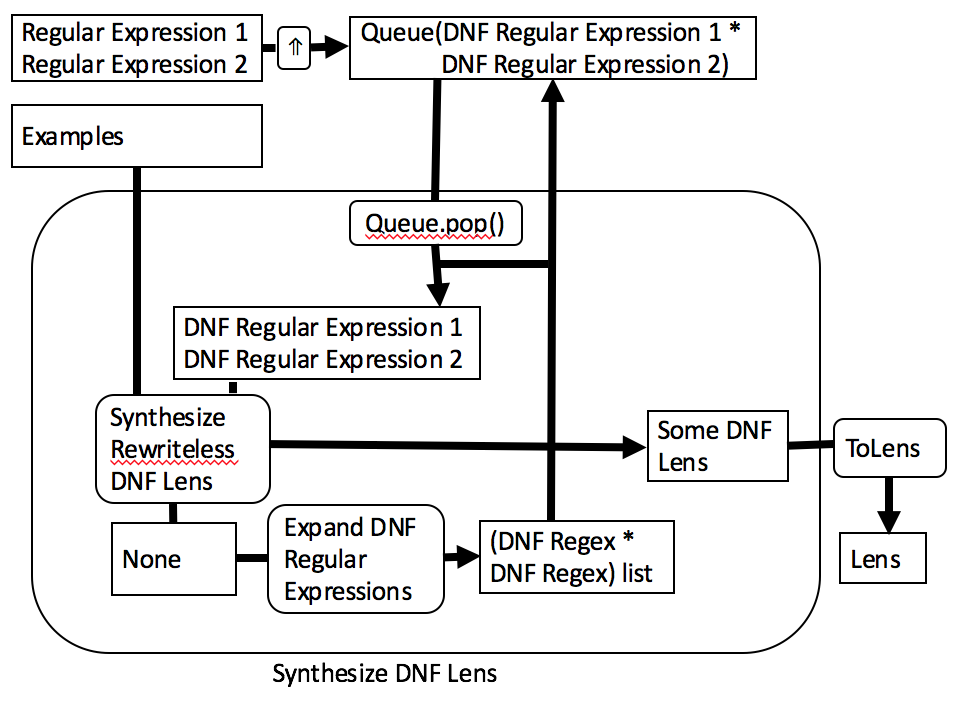
\includegraphics[scale=.5]{synth-lens-schematic.png}
  \begin{tikzpicture}[]
    \draw
    node at (0,0) [name=examples] {\scriptsize $\mathit{examples}$}
    node [name=input, right=.5cm of examples]{\scriptsize $(\Regex,\RegexAlt)$}
    node [draw, rectangle, name=todnfregex, right=.75cm of input] {$\ToDNFRegex$}
    node [draw, rectangle, name=emptyqueue, right=1cm of todnfregex] {\CF{Queue.Empty}}
    node [draw, rectangle, name=enqueue, below=.5cm of todnfregex]{\CF{Enqueue}}
    node [draw, rectangle, name=pop, below=1cm of enqueue] {\CF{Queue.Pop}}
    node [draw, rectangle, name=synthrewritelessdnf, below=4cm of examples] {\CF{SynthRewritelessDNF}}
    node [draw, rectangle, name=beautify, below=2cm of synthrewritelessdnf] {\CF{Beautify}}
    node [name=output, below=.5cm of beautify] {\scriptsize $\Lens$}
    node [draw, rectangle, name=rewrite, right=1.5cm of synthrewritelessdnf] {\CF{ApplyRewrites}}
    node [draw, rectangle, name=enqueuemany, above=.5cm of rewrite] {\CF{EnqueMany}}
    ;

    \draw[->] (input) -> (todnfregex);
    \draw[->] (todnfregex) -> (enqueue) node[midway,left] {\scriptsize $(\DNFRegex,\DNFRegexAlt)$};
    \draw[->] (emptyqueue) -> (enqueue);
    \draw[->] (enqueue) -> (pop) node[near end, left] {\scriptsize $Q$};
    \draw[->] (examples) -> (synthrewritelessdnf);
    \draw[->] (pop) -> (synthrewritelessdnf) node[midway,above=.3cm] {\scriptsize $(\DNFRegex,\DNFRegexAlt)$};
    \draw[->] (synthrewritelessdnf) -> (beautify) node[near end, right] {\scriptsize $\Lens$};
    \draw[->] (beautify) -> (output);
    \draw[->] (synthrewritelessdnf) -> (rewrite) node[midway,above] {\scriptsize $\mathit{None}$};
    \draw[->] (rewrite) -> (enqueuemany) node[midway,right] {\scriptsize $[(\DNFRegex_i,\DNFRegexAlt_i)]$};
    \draw[->] (pop) -> (enqueuemany) node[midway,right] {\scriptsize $Q$};
    \draw[-] (enqueuemany) -> (pop);
  \end{tikzpicture}

    
    \label{fig:synth-lens-schematic}
  \caption{Schematic Diagram for Lens Synthesis\afm{Schematic Diagram vs Code?}}
\end{figure}
The schematic diagram in 
Figure~\ref{fig:synth-lens-schematic} shows an overview of the synthesis
algorithm.  The algorithm, \PCF{SynthLens}, takes in a pair of
regular expressions, and examples, and uses $\ToDNFRegex$ to convert the
regular expressions into DNF regular expressions.
Then, \PCF{SynthDNFLens} is called on these DNF regular expressions to create a
DNF lens.
This DNF lens is then converted into a lens, and finally beautified for
readability.

\begin{algorithm}
  \caption{\PCF{SynthLens}}
  \begin{algorithmic}[1]
    \Function{SynthDNFLens}{$\DNFRegex,\DNFRegexAlt,\mathit{exs}$}
    \State $\mathit{Q} \gets \Call{SingletonQueue}{(\DNFRegex,\DNFRegexAlt),0}$
    \While{$\mathit{true}$}
    \State $(\mathit{q},\mathit{Q}) \gets \Call{Pop}{Q}$
    \State $((\DNFRegex,\DNFRegexAlt),\mathit{ExpCount}) \gets \mathit{q}$
    \State $\DNFLens \gets
    \Call{SynthRewritelessDNFLens}{\DNFRegex,\DNFRegexAlt,\mathit{exs}}$
    \If{$\DNFLens \neq \mathit{null}$}
    \State \textbf{return} $\DNFLens$
    \Else
    \State $\mathit{rxs} \gets \Call{ExpandOnce}{\DNFRegex,\DNFRegexAlt}$
    \State $\mathit{qs} \gets \Call{Map}{\lambda x.(x,\mathit{ExpCount}+1),\mathit{rxs}}$
    \State $\mathit{Q} \gets \Call{EnqueueMany}{\mathit{qs},\mathit{Q'}}$
    \EndIf
    \EndWhile
    \EndFunction
    \Statex
    \Function{SynthLens}{$\Regex,\RegexAlt,\mathit{exs}$}
    \State $(\DNFRegex,\DNFRegexAlt) \gets
    (\ToDNFRegexOf{\Regex},\ToDNFRegexOf{\RegexAlt})$
    \State $\DNFLens \gets \Call{SynthDNFLens}{\DNFRegex,\DNFRegexAlt,\mathit{exs}}$
    \State $\Lens \gets \Call{ToLens}{\DNFLens}$
    \State \textbf{return} $\Call{Beautify}{\Lens}$
    \EndFunction
  \end{algorithmic}
\end{algorithm}

In \PCF{SynthDNFLens}, a singleton priority queue is created, consisting of the
two input DNF regular expressions and the number of expansions preformed $(0)$.
This priority queue is designed
such that lower priority typing constraints either have undergone a large number
of rewrites, or have typing constraints that are very difference in appearance
from each other.
Next a loop is begun which pops the highest priority element from the queue.
This element is a tuple consisting of the DNF regular expressions, and a tracker
of how many expansions have been preformed.
\PCF{SynthRewritelessDNFLens} is then called on the DNF regular expressions and
the examples.
If a DNF lens is not found, it is returned.
If no lens is found, a single rewrite is applied to either the left or the right
DNF regular expression in \PCF{ExpandOnce}.  In other words, if $\DNFRegex$ and
$\DNFRegexAlt$ are the DNF regular expressions,
$\PCF{ExpandOnce}(\DNFRegex,\DNFRegexAlt) =
\SetOf{(\DNFRegex',\DNFRegexAlt) \SuchThat \DNFRegex \Rewrite \DNFRegex'}
\Union
\SetOf{(\DNFRegex,\DNFRegexAlt') \SuchThat \DNFRegexAlt \Rewrite \DNFRegexAlt'}$.
All the DNF regular expressions returned by this are enqueued, with the
information that an extra expansion has been preformed, and the loop continues.

\subsection{Priority Queue}
We say that the lower the priority value, the higher the priority.
The priority value of an element is based on two factors.  The first factor is
the number of expansions that have been performed.  If more expansions have been
preformed, the priority will be lower.  The inclusion of expansions preformed
forces some exploration of the
search space; if it were the only factor of priority, the search would be
entirely a breadth first search through the application of rewrite rules.
The second factor is how different the two regular expressions of the
specification are.  This difference is determined from our implementation of
a psuedometric $\Distance$.  Our distance $\Distance$ is
a pseudometric, as $\Distance$ satisfies the triangle property, $\Distance$ is
symmetric, and $\Distance(\DNFRegex,\DNFRegex) = 0$, but
$\Distance(\DNFRegex,\DNFRegexAlt) = 0$ does not imply $\DNFRegex =
\DNFRegexAlt$.  This pseudometric is implemented
as the sum of simpler pseudometrics,
$\Distance = \Distance_{size}+\Distance_{dist}$.

The size distance, $\Distance_{size}$ is defined as merely the difference in the
sizes of the DNF
regular expressions.  The size of a DNF regular expression is the sum of the
sizes of all lists present in the DNF regular expression data structure.
The size distance, $\Distance_{size}$ is formally defined as
$\Distance_{size}(\DNFRegex,\DNFRegexAlt)=\AbsOf{\Size(\DNFRegex)-\Size(\DNFRegexAlt)}$.
For two DNF regular expressions to have a rewriteless DNF lens between
them, they must be the same size, so using this pseudometric makes ones closer
in size popped sooner.

The distribution distance, $\Distance_{dist}$, captures how different the distributions of
user defined regular expressions in the two input regular expressions
are.
The distribution of user defined regular expressions can be viewed as
$\VectorSpace{}$, an
infinite dimensional vector space over the reals.
The set $\SetOf{1*(\RegexVariable,n) | n\in\Nats, \RegexVariable
  \text{ is a user defined regular expression}}$ serves as a basis for this
vector space.
DNF regular expressions with variables can map into this vector space with a function that
counts the number of user defined data types present at a given level.
This function, $\GetDist{}$ formalizes the mapping from DNF regular expressions
into $\VectorSpace$.

\begin{definition}\leavevmode\\
  \label{def:getdist}
  \begin{tabular}{@{}L@{}L@{}}
    \GetDist(\DNFOf{\Sequence_1;\ldots;\Sequence_n}) &
                                                       =\GetDist(\Sequence_1)+\ldots+\GetDist(\Sequence_n)\\
    \GetDist(\SequenceOf{\String_0;\Atom_1;\ldots;\Atom_n;\String_n}) &
                                                                        =\GetDist(\Atom_1)+\ldots+\GetDist(\Atom_n)\\
    \GetDist(\RegexVariable)&=1*(\RegexVariable,1)\\
    \GetDist(\IterateLensOf{\DNFLens})&=\phi(\GetDist(\DNFLens))
  \end{tabular}

  where $\phi$ is the linear map sending $1*(\RegexVariable,n)$ to
  $1*(\RegexVariable,n+1)$
\end{definition}

If $\LOneNorm$ computes the Manhattan distance on $\VectorSpace$,
$\Distance_{dist}(\DNFRegex,\DNFRegexAlt)=
\LOneNorm(\GetDist(\DNFRegex),\GetDist(\DNFRegexAlt))$.  This
distance calculates how different the distribution of user defined regular
expressions are in two DNF regular expressions.  Only when the distribution of
user defined regular expressions are equal can a lens between two DNF regular
expressions be synthesized.  This metric makes regular expressions with
similar distributions of user defined regular expressions be popped earlier.

The priority of a pair of DNF regular expressions, $(\DNFRegex{},\DNFRegexAlt{})$,
is $\Distance(\DNFRegex{},\DNFRegexAlt{})+8*\mathit{ExpansionCount}$, where
$\mathit{ExpansionCount}$ is the total number of expansions preformed.
Keeping track of expansion count is important as it allows for lower priority
expansions to be eventually popped, instead of getting stuck doing incorrect,
increasingly deep expansions whose DNF regular expressions have a low distance.
\afm{should i do an example, or is that going into too much detail?}
Experimentally, 8 is a good value for how much weight the expansion
count should get in the priority.  It allows for not getting stuck in a local
minima in the search space, while still allowing for the distance to choose the
correct expansion the majority of the time.

\subsection{SynthRewritelessDNF}

While performing type directed synthesis on DNF regular expressions, both
synthesizing a rewriteless DNF lens and synthesizing a Sequence lens requires
the generation of a permutation.  Naively searching through all possible
permutations is incredibly inefficient.  Were we to naively search through all the
rewriteless DNF Lenses between
the DNF regular expressions $\DNFOf{\Sequence_1;\ldots;\Sequence_n}$ and
$\DNFOf{\SequenceAlt_1;\ldots;\SequenceAlt_n}$, there would be $n!$ permutations
processed.

It is a better approach to recognize which subcomponents of types 
recognize which subcomponents of the types can be mapped to each other, and
create the permutations based on those mappings, than to
search through all possible permutations.  To handle finding which
subcomponents can be mapped to each other, SynthRewritelessDNF further
normalizes the input regular expressions.
Ordering the sequence subcomponents of a DNF lens further normalizes it.
Ordering the atom subcomponents of a DNF lens further normalizes it.
After correctly ordering the sequences, we can synthesize a rewriteless DNF lens
between $\DNFOf{\Sequence_1;\ldots;\Sequence_n}$ and
$\DNFOf{\SequenceAlt_1;\ldots;\SequenceAlt_n}$ merely through finding a sequence
lens between $\Sequence_i$ and $\SequenceAlt_i$ for all $i$.  Similarly, after
correctly ordering the atoms, we can
synthesize a rewriteless sequence lens 
between $\SequenceOf{\String_0;\Atom_1;\ldots;\Atom_n;\String_n}$ and
$\SequenceOf{\StringAlt_0;\AtomAlt_1;\ldots;\AtomAlt_n;\StringAlt_n}$ through
merely finding atom lenses between $\Atom_i$ and $\AtomAlt_i$ for all $i$.

However, these ordering normalization techniques can change the semantics of the
regular
expressions.  To get around this issue, remembering the alterations taken for
normalization, and later applying them in reverse to the synthesized DNF lens
can retrieve a lens between the original DNF regular expressions.

\begin{figure}
  \label{fig:lens-synth-ordering-ex}
  \centering
  \CF{Bib' <=> DNFEndUnroll}
  \begin{tikzpicture}
    \matrix (m) [matrix of nodes, row sep=1em, column sep=4em, minimum width=2em]
    {
      \CF{""} & $\Or$ & \CF{BibSequence2} \\
      \CF{""} & $\Or$ & \CF{BibSequence2} \\
      \CF{""} & $\Or$ & \CF{EndSequence2} \\
      \CF{""} & $\Or$ & \CF{EndSequence2} \\
    };
    \path[<->]
    (m-1-1) edge node [left] {} (m-2-1);
    \path[<->]
    (m-2-1) edge node [left] {} (m-3-1);
    \path[<->]
    (m-3-1) edge node [left] {} (m-4-1);
    \path[<->]
    (m-1-3) edge node [right] {} (m-2-3);
    \path[<->]
    (m-2-3) edge node [right] {\CF{lsequence}} (m-3-3);
    \path[<->]
    (m-3-3) edge node [right] {} (m-4-3);
  \end{tikzpicture}

  \CF{lsequence : BibSequence2 <=> EndSequence2}
  \begin{tikzpicture}
    \matrix (m) [matrix of nodes, row sep=1em, column sep=-.75em]
    {
      \CF{"author=\{"} & \Concat{}\CF{Name}\Concat{} & \CF{", "} &
      \Concat{}\CF{Name}\Concat{} & \CF{""} & \Concat{}\CF{Names}\Concat{} & \CF{""}
      & \Concat{}\CF{BibStar*}\Concat{} & \CF{"\},"}\\
      \CF{"author=\{"} & \Concat{}\CF{Name}\Concat{} & \CF{", "} &
      \Concat{}\CF{Name}\Concat{} & \CF{""} & \Concat{}\CF{Names}\Concat{} & \CF{""}
      & \Concat{}\CF{BibStar*}\Concat{} & \CF{"\},"}\\
      \CF{"\%A "} & \Concat{}\CF{Name}\Concat{} & \CF{""} &
      \Concat{}\CF{Name}\Concat{} & \CF{" "} & \Concat{}\CF{Names}\Concat{} & \CF{""}
      & \Concat{}\CF{EndStar*}\Concat{} & \CF{""}\\
      \CF{"\%A "} & \Concat{}\CF{Name}\Concat{} & \CF{""} &
      \Concat{}\CF{Names}\Concat{} & \CF{" "} & \Concat{}\CF{Name}\Concat{} & \CF{""}
      & \Concat{}\CF{EndStar*}\Concat{} & \CF{""}\\
    };
    \path[<->]
    (m-1-2) edge node [right] {} (m-2-4);
    \path[<->]
    (m-1-4) edge node [right] {} (m-2-2);
    \path[<->]
    (m-1-6) edge node [left] {} (m-2-6);
    \path[<->]
    (m-1-8) edge node [left] {} (m-2-8);
    \path[<->]
    (m-2-2) edge node [right] {} (m-3-2);
    \path[<->]
    (m-2-4) edge node [right] {} (m-3-4);
    \path[<->]
    (m-2-6) edge node [left] {} (m-3-6);
    \path[<->]
    (m-2-8) edge node [right] {\CF{lstar}} (m-3-8);
    \path[<->]
    (m-3-2) edge node [right] {} (m-4-2);
    \path[<->]
    (m-3-4) edge node [right] {} (m-4-6);
    \path[<->]
    (m-3-6) edge node [left] {} (m-4-4);
    \path[<->]
    (m-3-8) edge node [right] {} (m-4-8);
  \end{tikzpicture}

  \CF{lstar : BibStar <=> EndStar}
  \begin{tikzpicture}
    \matrix (m) [matrix of nodes, row sep=1em, column sep=-.75em]
    {
      \CF{" and "} & \Concat{}\CF{Name}\Concat{} & \CF{", "} &
      \Concat{}\CF{Name}\Concat{} & \CF{""} & \Concat{}\CF{Names}\Concat{} &
      \CF{""}\\
      \CF{" and "} & \Concat{}\CF{Name}\Concat{} & \CF{", "} &
      \Concat{}\CF{Name}\Concat{} & \CF{""} & \Concat{}\CF{Names}\Concat{} &
      \CF{""}\\
      \CF{"\%A "} & \Concat{}\CF{Name}\Concat{} & \CF{""} &
      \Concat{}\CF{Name}\Concat{} & \CF{" "} & \Concat{}\CF{Names}\Concat{}
      & \CF{""}\\
      \CF{"\%A "} & \Concat{}\CF{Name}\Concat{} & \CF{""} &
      \Concat{}\CF{Names}\Concat{} & \CF{" "} & \Concat{}\CF{Name}\Concat{}
      & \CF{""}\\
    };
    \path[<->]
    (m-1-2) edge node [right] {} (m-2-4);
    \path[<->]
    (m-1-4) edge node [left] {} (m-2-2);
    \path[<->]
    (m-1-6) edge node [left] {} (m-2-6);
    \path[<->]
    (m-2-2) edge node [right] {} (m-3-2);
    \path[<->]
    (m-2-4) edge node [left] {} (m-3-4);
    \path[<->]
    (m-2-6) edge node [left] {} (m-3-6);
    \path[<->]
    (m-3-2) edge node [right] {} (m-4-2);
    \path[<->]
    (m-3-4) edge node [left] {} (m-4-6);
    \path[<->]
    (m-3-6) edge node [left] {} (m-4-4);
  \end{tikzpicture}
  \caption{Synthesized Lens Mappings from Orderings}
\end{figure}

Consider the example of synthesizing a lens between \CF{Bib'} and
\CF{DNFEndUnroll}, shown in Figure~\ref{fig:lens-synth-ordering-ex}.
The top layer (the original DNF regular expression subparts for BibTex) maps
into the second layer through an ordering of its subparts.
The bottom layer (the original DNF regular expression subparts for EndNote) maps
into the third layer through an ordering of its subparts.
The second and third layer are mapped to each other by merely zipping together
the subparts.
The composition of the orderings done in each layer combines to make
the permutations required for the lens between unordered BibTex and unordered
EndNote.

Unfortunately, while this ordering and mapping procedure can find a well typed
DNF lens, it doesn't
necessarily find the one that matches the examples.  In the situation where
there are multiple valid sorted orderings, there are multiple different lenses
with potentially different semantics.  For example, in the
synthesis of a lens between \CF{BibStar} and \CF{EndStar}, there are two
instances of \CF{Name}.  Which of these should go first when ordered?  Instead
of iterating through all the possible sortings, and finding one that matches
the examples, we would like to
be able to immediately find only a sorting which satisfies the examples.

The key insight here is that certain invariants must hold for a DNF lens to have
semantics that match the examples.

\begin{enumerate}
\item If a source example string matches one of the sequences during parsing,
  it must be sent to the sequence the target example string matches during parsing.
\item If a source example string matches a user defined regular expression during
  parsing, the target must match the exact same string during parsing.
\item If a source example string matches an iteration, then the target must iterate
  the same number of times, and all the invariants must hold for each iterated part.
\end{enumerate}

We can hold these invariants by joining additional parsing information alongside
the regular
expression components, and creating an ordering on DNF regular expressions
with parsing information.  By attaching additional parsing information,
each \CF{Name} no longer is merely a \CF{Name}, it is \CF{Name} alongside
\CF{"Stephen"} or \CF{"Kleene"}.  With that additional information, the
\CF{Name}s can be ordered, and correctly mapped to the other
\CF{Name}s in a manner that satisfies the examples.


% end implementation


% begin evaluation
\section{Evaluation}
\label{evaluation}

\begin{figure*}
  \centering
  \begin{tabular}{|c|c|c|c|c|}
    \hline
    \bfseries Test & \bfseries Computation Time (s)
    & \bfseries No UserDef Time (s) & \bfseries Exs Reqd & \bfseries Max Exs Reqd
                                   \csvreader[head to column names]{generated-data/data.csv}{}
                                   {\\\hline\Test & \ComputationTime  & \ForceExpandTime & \ExamplesRequired & \MaxExampleCount}
    \\\hline
  \end{tabular}
  \label{fig:evaluation-data}
\end{figure*}

We evaluated our algorithm by testing its ability to synthesize bijective lenses
that would be seen in practice.  As such, we derived the bijective lens synthesis problems
from string and data transformation problems present in the Augeas
repository, from FlashFill examples, and from Boomerang's test suite.
Furthermore, through generating random examples, we test the importance of
examples.  Through removing all user input user defined data type information,
we test the importance of user defined data types to our algorithm.
Figure~\ref{fig:evaluation-data} presents the data from our test runs.
The values presented are the arithmetic means of 10 test runs.
The tests were run on a 2.5 GHz Intel Core i7 processor, with
16 GB of 1600 MHz DDR3, running Mac OS X Yosemite.

\subsection{Test Selection}

Our tests were modified from examples of string transformations found in Augeas,
Boomerang, and FlashFill.

Augeas uses combinators similar to Boomerang, but enables transformations of the
data into a structured format, instead of merely a string format.  We mimicked
these in our lens synthesis problems by making the output formats look like
the a serialized version of the structure.  Furthermore, Augeas is able to
handle all lenses,
where the synthesis algorithm can only synthesize bijective ones.  By including
more fields data format on the right, we were able to turn non-bijective lenses
into bijective ones.

Just like Augeas, Boomerang has combinators that go beyond the basic lens
combinators, including keyed data and quotienting.  Keyed data has little impact
on the output format, but merely changes how the invertibility laws behave.  Because
we have bijective lenses, keyed data has no impact.  We treat quotienting
similarly to non-bijective lenses.  Any part of the string that would be
quotiented, instead is included in a different area of the string, to maintain
bijectivity.

FlashFill examples, unlike the other tests, are not in fact lenses, they are
merely string transformations.  Furthermore, many of them are non-bijective, as
FlashFill examples are often about extracting certain pieces of information.
However, through the same process of making the transformations bijective as
tackled in other ports, we
add in invertibility constraints that allow the transformation to be interpreted
as a lens.

These tests were selected to demonstrate our algorithms ability to synthesize
transformations used in practice.  Many had an appearance similar to the
\CF{BibEnd} example given in Figure~\ref{fig:bibend-spec}.  However, \CF{BibEnd}
was simplified for clarity's sake, and the examples taken from real world
applications are usually much longer and involve far more user defined regular
expressions.  Furthermore, in larger synthesis problems,
we build intermediary lenses
between intermediary regular expressions as a sanity check for bijectivity.
These intermediary lenses are then used in the synthesis algorithm for mapping
the intermediary sub-expressions, to avoid repeating the same synthesis
algorithm.

\subsection{Speed of Synthesis}
Figure~\ref{fig:evaluation-data} provides the runtime of our algorithm on our
test suite, with the column \textbf{ComputationTime} showing the runtime of the
overall synthesis algorithm.

In this figure, we want to minimize runtime, as a smaller runtime means we were
able to synthesize very efficiently.
We found that, on many of our difficult examples, our algorithm was able to find
the appropriate lens very quickly.

This figure shows us where the strengths and weaknesses of our algorithm lie.
In particular, our synthesis strategy does quite well on problems that only
include a small number of transformations, even if the number of sequences is
decently large.
There are two tests where our algorithm is weaker, however.  The test
double-capitalization-problem.ls, and the test xml.ls are both quite slow.

The test double-capitalization-problem.ls was intentionally made to be slow to
exploit an issue that can arise from DNF conversion.  In converting to DNF form,
a concatenation of many \OrRegexType{}s causes a huge blowup.  In
double-capitalization-problem.ls, this blowup is exploited.  This problem causes a
blowup, causing there to be 676 sequences created immediately.
Any time SynthRewritelessDNF is called, it must find the correct mapping of all
676 sequences.  A single instance of finding 676 sequences is not that bad, but it
becomes worse when that must be done on every expansion, and some of the bad
expansions that are popped create 17576 sequences.
If we take this problem to the logical extremes, we see that the the triple
capitalization problem takes 6.974 seconds, and the quadruple capitalization
problem takes 33 minutes and 54.730 seconds.

The test xml.ls takes a long time, as it is a very complicated regular
expression.  Because full xml is not expressible as a regular expression, xml.ls
expresses xml of depth up to 3.  The full specification for all xml up to depth
3 is a huge regular expression.  Not only
this is the regular expression large,
but a number of regular expression expansions must be preformed to get it
into dictionary form; different things must happen on a star that is matched
0 times, and a star that is matched one or more times.  Because of the size of
the regular expression, many expansions can be preformed, and because expansions
must be preformed, it requires a large amount of search to find the correct
expansions to synthesize a lens.

\subsection{Importance of Examples}

We wanted to see how many examples were required to synthesize the correct
bijective lens.
However, because of our implicit understanding of the algorithm, we fear we may
choose examples that we know will work well with the synthesis algorithm,
instead of choosing examples that users are likely to.
Because of that, we test the number of examples that it takes to generate the
correct lens, with randomly generated examples.

The column \textbf{Examples Required} in Figure~\ref{fig:evaluation-data}
provides the number of randomly generated examples it takes, on average, to
synthesize the correct lens on our test suite.  

As we see in Figure~\ref{fig:evaluation-data}, examples are not
incredibly
important for synthesizing bijective lenses.
Because bijective lenses have very few well typed programs, compared to the
number of functions, oftentimes just a few examples is sufficient.
As would be expected, the functions that have to make choices about the
locations of where data goes are those that require more examples.
In particular, the address problem requires more examples, because it must make
choices of where information goes, like which name is the a person's first name,
and which is their last.

However, this column does not tell the whole story.
The column \textbf{Max Exs Reqd} in Figure~\ref{fig:evaluation-data}
provides the maximum number of examples required.
This column represents the number of examples that are required if the
synthesis engine always guessed the incorrect permutation, when multiple
permutations satisfy the type and examples.
This column shows that, while in practice few examples are required,
when complicated permutations are needed, more examples are required.

The test programs require
so few examples, when adversarial synthesis of permutations could necessitate so
many examples, because we unintentionally ordered the $\OrRegexType$s in many of
the test programs regular expressions.
We represented subparts of similar data formats in a consistent ordering,
requiring fewer examples.  We expect that most programmers do the same.
Maintaining similar subparts in similar orderings makes the types much easier to
read, make it easier for checking that the languages are in bijection with each
other.

\subsection{Importance of User Defined Data Types}

User defined data types are very critical to the algorithm and performance of
the synthesis algorithm.  User defined data types help direct the search of
which expansions should be performed.  Furthermore, they help to reduce the
number of sequences we have to deal with.  There is a potentially exponentially
large blowup in converting regular expressions into DNF form, but keeping
certain portions of the regular expressions abstracted lessens that blowup,
as those regular expressions are kept atomic in converting into DNF form.

User defined data types are also critical in the applications of previously
defined lenses.  We restrict the application of previously defined lenses to
only on user defined data types in the synthesis algorithm.  We then group the
user defined data types based on which have previously defined lenses between
them.  This grouping allows for efficient recognition of when two user defined regular
expressions can be mapped to each other.  Removing the ability to use previously
defined lenses makes certain problems intractable, like xml.ls.

While we can simulate the use of user defined data types automatically, by
giving regular expressions which have the same syntax the same user defined data
type, manually inputting them performs better in practice.  The
procedure for automatically creating user defined data types creates far more
data types, which then creates a more complicated search problem.

\subsection{Impact of Incompleteness to Full Regular Expression Equivalence}
We found that not being able to synthesize lenses where retyping used full
regular expression equivalence was not a detriment to the algorithm at all.  The
only regular expression equivalences that naturally occured were ones that we
had already incorporated in our equivalences.

This lack of impact is likely because, when the languages of two regular expressions have
bijective lenses between them, the data is naturally grouped in similar ways on each
side of the regular expression.  If there was a block of text, it would likely
be written on both sides as \CF{Character*}, instead of \CF{(A*notA)*A*}, where
\CF{A} is the character \CF{A}, and \CF{notA} is all characters except for
\CF{A}.  If for some reason it were important that \CF{A} and \CF{notA} were
separated, we found that it would be important in both data representations.
The only places where \StarRegexType{} equivalences were used was in
differentiating number of iterations, and in placing separators, the
equivalences of which are already accounted for in $\DefinitionalEquiv$.
% end evaluation

% begin discussion
\subsection{Discussion}

We found that in practice, requiring a user to put in more information for the
synthesis of a string transformation creates a more reliable algorithm, which
also requires fewer examples.
However, these benefits comes at a few costs: the user needs to know how to write out
regular expressions, and the user must spend the time writing out the regular
expressions, and must do so correctly.  However, for our use case of a
programmer working on enterprise software, these additional costs are minor.

The largest difficulty the use of this program is the restriction to bijective lenses.
Oftentimes, we find the need to hide information away in some alternate form.
For example, there is oftentimes whitespace in the definition of a regular
expression.  This whitespace must be copied somehow over to the other side.
Oftentimes copying whitespace requires the use of having a portion of the string dedicated to
holding the whitespace information of the other side.

Another annoyance is the fact that if the correct lens does not exist,
rarely does the tool terminate.  Much of the time it will just spin trying to
perform increasingly complicated regular expression transformations to find the
correct lens.
A better solution would be to find something close to the correct lens, and have
a user interaction model that supports iterative synthesis.  The user could give
more examples which fix where the program is wrong.
% end discussion


% begin related-work
\section{Related Work}
\subsection{FlashFill}
FlashFill is another string transformation program.  FlashFill takes input and
output examples as its only form of specification.  For FlashFill's primary use
case, providing easy transformations of Excel data, input and output examples as
the only specification makes a lot of sense.  Our tool is intended for use for
programmers to use, who already know regular expressions.  Our tool is oriented
towards a situation where a programmer would check the generated code into a
repository.  From requiring this extra information, our tool is able to handle
synthesize complicated functions that go beyond what FlashFill can synthesize.
For example, given 21 examples of extracting the first author, with the names
reversed, FlashFill still gave incorrect outputs for a number of inputs, even
when those inputs are a similar form to the provided examples.

Furthermore, even if FlashFill were to synthesize the correct program, it would
be foolhardy to check the generated code into a repository.  FlashFill does not
fail on inputs it doesn't know how to handle, rather it tries to provide an
output.  This model is different from the generated lenses, which will quickly
fail on inputs that do not match it's intended specification.  Furthermore, the
specification of what inputs should be handled are provided by the user, not
inferred from the examples, giving it more reliability.

Furthermore, FlashFill is unable to synthesize programs with nexted loops
without custom configuration.  The lack of nested loops was a pragmatic choice
in allowing FlashFill
to efficiently find many correct transformations very quickly.  However, in
many complicated data formats, nested loops are inevitable. 

\subsection{FlashExtract}
FlashExtract is a program that takes an input of a string, and a partial
labeling of substrings within that string, to try to label the rest of the
substrings.  FlashExtract was able to label some amounts of the strings, but was
unable to handle reorderings of the data well.  While it would do well in
extracting data when the data came in the same form, for example, when given a
Bibtex file where the fields come in a specific order, the data would do well,
however, FlashExtract was unable to handle when fields were given in different
orders, even if previous examples in that order were given.

The schemas for FlashExtract are not customized for data formats which have many
\OrRegexType{}s.  In particular, there is no \OrRegexType{} schema at all!  The
only way that \OrRegexType{}s can be simulated is through the concatenation of
all the choices, where all but one of the choices becomes \CF{null} on each
application.  However, this concatenation strategy is only a hack, and as such,
FlashExtract preforms badly on
circumstances that require \OrRegexType{}s.
Indeed, after providing 30 examples of BibTex
examples, FlashExtract was still unable to generalize to correctly extract
the fields of a BibTex example.
% end related-work

% begin conclusion
\section{Conclusion}

We have coded up an implementation of type-directed synthesis on a domain
specific language of bijective lenses.  This program allows users to input two
regular expressions, and a few input/output examples, and will synthesize a
bijective lens between those regular expressions, matching those input/output
examples.  While lenses are very useful for their guarantees, they are a
difficult domain specific language to code in, in practice.  This program
provides an easier interaction model for the creation of lenses through using
synthesis as the way to interact with the programmer.

This synthesis algorithm is competitive with state of the art tools for
synthesis on strings transformations, and is better at synthesizing very
complicated transformations.  The additional capabilities are gained through requiring a
larger amount of user interaction with the synthesis algorithm.  However,
for this increased interaction, the program provides the capabilities of
synthesizing very complicated transformations, and provides stronger guarantees
about correctness on inputs dissimilar to those provided in the examples.

\subsection{Future Work}
Some of the issues seen in this work have already been noted.  For example, in the
quotient lens paper, the issue of having to hack a place in the source string to
move whitespace information from the view to the source was noted.  An extension
we would like to work on would be able to synthesize quotient lenses.

Another approach to having disparate information on each side of the lens is
through the use of symmetric lenses.  Symmetric lenses could be another approach to the
whitespace problem.

% end conclusion

\appendix

\ifanon\else
\acks 
% Expeditions in Computer Augmented Program Engineering (ExCAPE, NSF
% Award CCF-1138996).
% Acknowledgments, if needed.
\finish{Write me.  Mention all relevant grants, esp. DARPA.}
\fi

% We recommend abbrvnat bibliography style.

\bibliographystyle{abbrvnat}

% The bibliography should be embedded for final submission.

\bibliography{local}

% Appendices.

\onecolumn
% begin proofs
\section{Proofs}
% proof-dnfrc start
% First we will prove some lemmas.
\begin{lemma}[Equivalence of \ConcatSequence{} and \Concat{}]
  If $\LanguageOf{\Regex}=\LanguageOf{\Sequence}$,
  and $\LanguageOf{\RegexAlt}=\LanguageOf{\SequenceAlt}$,
  then $\LanguageOf{\RegexConcat{\Regex}{\RegexAlt}}=\LanguageOf{\ConcatSequenceOf{\Sequence}{\SequenceAlt}}$.
\end{lemma}
\begin{proof}
  Let $\Sequence=\SequenceOf{\String_0\SequenceSep\Atom_1\SequenceSep\ldots
    \SequenceSep\Atom_n\SequenceSep\String_n}$, and
  let\\ $\SequenceAlt=[\StringAlt_0\SequenceSep\AtomAlt_1\SequenceSep\ldots
  \SequenceSep\AtomAlt_m\SequenceSep\StringAlt_m]$\\
  \begin{tabular}{@{}L@{}L@{}}
    \LanguageOf{\ConcatSequenceOf{\Sequence}{\SequenceAlt}} & = 
                                                              \LanguageOf{\SequenceOf{\String_0\SequenceSep\Atom_1\SequenceSep\ldots
                                                              \SequenceSep\Atom_n\SequenceSep\String_n\Concat\StringAlt_0\SequenceSep{}
                                                              \AtomAlt_1\SequenceSep\ldots\SequenceSep\AtomAlt_m\SequenceSep\StringAlt_m}} \\
                                                            & = 
                                                              \{\String_0\Concat\String_1'\Concat\ldots\Concat\String_n'\Concat\String_n
                                                              \Concat\StringAlt_0\Concat\StringAlt_1'\Concat\ldots
                                                              \Concat\StringAlt_m'\Concat\StringAlt_m \\
                                                            & \hspace{5em} \SuchThat{} \String_i'\in\LanguageOf{\Atom_i} \BooleanAnd{}
                                                              \StringAlt_i'\in\LanguageOf{\AtomAlt_i}\}\\
                                                            & = 
                                                              \{\String\Concat\StringAlt{} \SuchThat{} \String\in\LanguageOf{\Sequence}
                                                              \BooleanAnd{} \StringAlt\in\LanguageOf{\SequenceAlt}\}\\
                                                            & =
                                                              \{\String\Concat\StringAlt{} \SuchThat{} \String\in\LanguageOf{\Regex}
                                                              \BooleanAnd{} \StringAlt\in\LanguageOf{\RegexAlt}\}\\
                                                            & =
                                                              \LanguageOf{\RegexConcat{\Regex}{\RegexAlt}}
  \end{tabular}
\end{proof}

\begin{lemma}[Equivalence of \ConcatDNF{} and \Concat{}]
  \label{lem:cdnfeq}
  If $\LanguageOf{\Regex}=\LanguageOf{\DNFRegex}$,
  and $\LanguageOf{\RegexAlt}=\LanguageOf{\DNFRegexAlt}$,
  then $\LanguageOf{\RegexConcat{\Regex}{\RegexAlt}}=
  \LanguageOf{\ConcatDNFOf{\DNFRegex}{\DNFRegexAlt}}$.
\end{lemma}
\begin{proof}
  Let $\DNFRegex=\DNFOf{\Sequence_0\DNFSep\ldots\DNFSep\Sequence_n}$, and
  let $\DNFRegexAlt=\DNFOf{\SequenceAlt_0\DNFSep\ldots\DNFSep\SequenceAlt_m}$
  \begin{tabular}{@{}L@{}L@{}}
    \LanguageOf{\ConcatDNFOf{\DNFRegex}{\DNFRegexAlt}} & = 
                                                         \LanguageOf{\DNFOf{\ConcatSequenceOf{\Sequence_i}{\SequenceAlt_j}
                                                         \text{ for $i\in\RangeIncInc{1}{n}$, $j\in\RangeIncInc{1}{m}$}}} \\
                                                       & = 
                                                         \{\String\SuchThat \String\in\ConcatSequenceOf{\Sequence_i}{\SequenceAlt_j}\\
                                                       & \hspace{5em}
                                                         \text{ where $i\in\RangeIncInc{1}{n}$, $j\in\RangeIncInc{1}{m}$}\}\\
                                                       & = 
                                                         \{\String\Concat\StringAlt{} \SuchThat{} \String\in\LanguageOf{\Sequence_i}
                                                         \BooleanAnd{} \StringAlt\in\LanguageOf{\SequenceAlt_j}\}\\
                                                       & \hspace{5em}
                                                         \text{ where $i\in\RangeIncInc{1}{n}$, $j\in\RangeIncInc{1}{m}$}\}\\
                                                       & =
                                                         \{\String\Concat\StringAlt{} \SuchThat{} \String\in\LanguageOf{\DNFRegex}
                                                         \BooleanAnd{} \StringAlt\in\LanguageOf{\DNFRegexAlt}\}\\
                                                       & =
                                                         \{\String\Concat\StringAlt{} \SuchThat{} \String\in\LanguageOf{\Regex}
                                                         \BooleanAnd{} \StringAlt\in\LanguageOf{\RegexAlt}\}\\
                                                       & =
                                                         \LanguageOf{\RegexConcat{\Regex}{\RegexAlt}}
  \end{tabular}
\end{proof}

\begin{lemma}[Equivalence of $\Atom$ and $\AtomToDNFOf{\Atom}$]
  \label{lem:atomtodnfeq}
  $\LanguageOf{\Atom} = \LanguageOf{\AtomToDNFOf{\Atom}}$
\end{lemma}
\begin{proof}
  $\LanguageOf{\AtomToDNFOf{\Atom}} =
  \LanguageOf{\DNFOf{\SequenceOf{\EmptyString;\Atom;\EmptyString}}}$

  $\LanguageOf{\DNFOf{\SequenceOf{\EmptyString;\Atom;\EmptyString}}} =
  \SetOf{\String \SuchThat \String \in
    \LanguageOf{\SequenceOf{\EmptyString;\Atom;\EmptyString}}}$.

  $\LanguageOf{\SequenceOf{\EmptyString;\Atom;\EmptyString}} =
  \SetOf{\EmptyString\Concat\String\Concat\EmptyString \SuchThat \String \in
    \LanguageOf{\Atom}} = \SetOf{\String \SuchThat \String \in
    \LanguageOf{\Atom}} = \LanguageOf{\Atom}$.

  This means $\LanguageOf{\DNFOf{\SequenceOf{\EmptyString;\Atom;\EmptyString}}}
  = \SetOf{\String \SuchThat \String \in \LanguageOf{\Atom}} =
  \LanguageOf{\Atom}$.
\end{proof}

\begin{lemma}[Equivalence of \OrDNF{} and \Or{}]
  \label{lem:odnfeq}
  If $\LanguageOf{\Regex}=\LanguageOf{\DNFRegex}$,
  and $\LanguageOf{\RegexAlt}=\LanguageOf{\DNFRegexAlt}$,
  then $\LanguageOf{\RegexOr{\Regex}{\RegexAlt}}=
  \LanguageOf{\OrDNFOf{\DNFRegex}{\DNFRegexAlt}}$.
\end{lemma}
\begin{proof}
  Let $\DNFRegex=\DNFOf{\Sequence_0\DNFSep\ldots\DNFSep\Sequence_n}$, and
  let $\DNFRegexAlt=\DNFOf{\SequenceAlt_0\DNFSep\ldots\DNFSep\SequenceAlt_m}$
  \begin{tabular}{@{}L@{}L@{}}
    \LanguageOf{\OrDNFOf{\DNFRegex}{\DNFRegexAlt}} & = 
                                                     \LanguageOf{\DNFOf{\Sequence_0\DNFSep\ldots\DNFSep\Sequence_n\DNFSep
                                                     \SequenceAlt_1\DNFSep\ldots\DNFSep\SequenceAlt_m}}\\
                                                   & = 
                                                     \{\String\SuchThat{} \String\in\Sequence_i\vee\String\in\SequenceAlt_j\\
                                                   & \hspace{5em}
                                                     \text{ where $i\in\RangeIncInc{1}{n}$, $j\in\RangeIncInc{1}{m}$}\}\\
                                                   & = 
                                                     \{\String{} \SuchThat{} \String\in\LanguageOf{\DNFRegex}
                                                     \BooleanOr{} \String\in\LanguageOf{\DNFRegexAlt}\}\\
                                                   & =
                                                     \{\String \SuchThat{} \String\in\LanguageOf{\Regex}
                                                     \BooleanOr{} \String\in\LanguageOf{\RegexAlt}\}\\
                                                   & =
                                                     \LanguageOf{\RegexOr{\Regex}{\RegexAlt}}
  \end{tabular}\\
\end{proof}

\dnfrc*
\begin{proof}
  By structural induction.

  Let $\Regex=\String$.
  $\LanguageOf{\ToDNFRegex(\String)}=\LanguageOf{\DNFOf{\SequenceOf{\String}}}=
  \{\String\}=\LanguageOf{\String}$

  Let $\Regex=\emptyset$.
  $\LanguageOf{\ToDNFRegex(\emptyset)}=\LanguageOf{\DNFOf{}} =
  \{\} = \LanguageOf{\emptyset}$.

  Let $\Regex=\StarOf{\Regex'}$.
  By induction assumption, $\LanguageOf{\ToDNFRegex(\Regex')}=
  \LanguageOf{\Regex'}$.\\
  \begin{tabular}{@{}L@{}L@{}}
    \LanguageOf{\ToDNFRegex(\StarOf{\DNFRegex'})} & =
                                                    \LanguageOf{\DNFOf{\SequenceOf{\StarOf{\ToDNFRegex(\Regex')}}}}\\
                                                  & =
                                                    \{\String\SuchThat\String\in
                                                    \LanguageOf{\SequenceOf{\StarOf{\ToDNFRegex(\Regex')}}}\}\\
                                                  & = 
                                                    \{\String\SuchThat{} \String\in\LanguageOf{\StarOf{\ToDNFRegex(\Regex')}}\}\\
                                                  & =
                                                    \{\String_1\Concat\ldots\Concat\String_n\SuchThat{}
                                                    n\in\Nats\\
                                                  & \hspace*{3em}\BooleanAnd\String_i\in\LanguageOf{\ToDNFRegex(\Regex')}\}\\
                                                  & =
                                                    \{\String_1\Concat\ldots\Concat\String_n\SuchThat{}
                                                    n\in\Nats\BooleanAnd\String_i\in\LanguageOf{\Regex'}\}\\
                                                  & = \LanguageOf{\StarOf{\Regex'}}
  \end{tabular}

  Let $\Regex=\RegexConcat{\Regex_1}{\Regex_2}$.
  By induction assumption,
  $\LanguageOf{\ToDNFRegex(\Regex_1)}=\LanguageOf{\Regex_1}$, and
  $\LanguageOf{\ToDNFRegex(\Regex_2)}=\LanguageOf{\Regex_2}$.
  $\ToDNFRegex(\RegexConcat{\Regex_1}{\Regex_2})=
  \ConcatDNFOf{\ToDNFRegex(\Regex_1)}{\ToDNFRegex(\Regex_2)}$.
  By Lemma~\ref{lem:cdnfeq},
  $\RegexConcat{\Regex_1}{\Regex_2}=
  \ConcatDNFOf{\ToDNFRegex(\Regex_1)}{\ToDNFRegex(\Regex_2)}$.

  Let $\Regex=\RegexOr{\Regex_1}{\Regex_2}$.
  By induction assumption,
  $\LanguageOf{\ToDNFRegex(\Regex_1)}=\LanguageOf{\Regex_1}$, and
  $\LanguageOf{\ToDNFRegex(\Regex_2)}=\LanguageOf{\Regex_2}$.
  $\ToDNFRegex(\RegexOr{\Regex_1}{\Regex_2})=
  \OrDNFOf{\ToDNFRegex(\Regex_1)}{\ToDNFRegex(\Regex_2)}$.
  By Lemma~\ref{lem:odnfeq},
  $\RegexOr{\Regex_1}{\Regex_2}=
  \OrDNFOf{\ToDNFRegex(\Regex_1)}{\ToDNFRegex(\Regex_2)}$.
\end{proof}
% proof-dnfrc end



% proof-dnfrs start
% First we will prove some lemmas.
\begin{lemma}
  \label{lem:sequence-rx}
  Let $\SequenceOf{\String_0\SequenceSep\Atom_1\SequenceSep
    \ldots\Atom_n\SequenceSep\String_n}$ be a sequence,
  and\\
  $\ToDNFRegex(\ToRegex(\Atom_i))=\DNFOf{\SequenceOf{\Atom_i}}$.
  Then,\\$\ToDNFRegex(\ToRegex(\SequenceOf{\String_0\SequenceSep\Atom_1\SequenceSep
    \ldots\Atom_n\SequenceSep\String_n}))=$\\
  $\DNFOf{\SequenceOf{\String_0\SequenceSep\Atom_1\SequenceSep
      \ldots\Atom_n\SequenceSep\String_n}}$.
\end{lemma}
\begin{proof}
  By induction on $n$.

  Let $n=0$.
  $\Sequence=\SequenceOf{\String_0}$.\\
  $\ToDNFRegex(\ToRegex(\SequenceOf{\String_0}))=
  \ToDNFRegex(\String_0)=\DNFOf{\SequenceOf{\String_0}}$

  Let $n>0$,
  $\Sequence=\SequenceOf{\String_0\SequenceSep\Atom_1\SequenceSep
    \ldots\Atom_n\SequenceSep\String_n}$.\\
  $\ToDNFRegex(\ToRegex(\SequenceOf{\String_0\SequenceSep\Atom_1\SequenceSep
    \ldots\Atom_n\SequenceSep\String_n}))$\\
  $\ToDNFRegex(\ToRegex(\SequenceOf{\String_0\SequenceSep\Atom_1\SequenceSep
    \ldots\Atom_{n-1}\SequenceSep\String_{n-1}})\Concat\ToRegex(\Atom_n)
  \Concat\String_n)$=\\
  $\ToDNFRegex(\ToRegex(\SequenceOf{\String_0\SequenceSep\Atom_1\SequenceSep
    \ldots\Atom_{n-1}\SequenceSep\String_{n-1}}))
  \ConcatDNF\\
  \ToDNFRegex(\ToRegex(\Atom_n))
  \ConcatDNF\\
  \ToDNFRegex(\String_{n-1})$=
  $\DNFOf{\SequenceOf{\String_0\SequenceSep\Atom_1\SequenceSep
      \ldots\Atom_{n-1}\SequenceSep\String_{n-1}}}
  \ConcatDNF\\
  \DNFOf{\SequenceOf{\Atom_n}}
  \ConcatDNF
  \DNFOf{\SequenceOf{\String_n}}$=
  $\DNFOf{\SequenceOf{\String_0\SequenceSep\Atom_1\SequenceSep
      \ldots\Atom_n\SequenceSep\String_n}}$.
\end{proof}



\begin{lemma}
  \label{lem:dnf-rx}
  Let $\DNFOf{\Sequence_1\DNFSep\ldots\DNFSep\Sequence_n}$ be a sequence,
  and\\ $\ToDNFRegex(\ToRegex(\Sequence_i))=\DNFOf{\Sequence_i}$.
  Then,\\ $\ToDNFRegex(\ToRegex(\DNFOf{\Sequence_1\DNFSep\ldots\DNFSep\Sequence_n}))=
  \DNFOf{\Sequence_1\DNFSep\ldots\DNFSep\Sequence_n}$.
\end{lemma}
\begin{proof}

  By induction on $n$.

  Let $n=0$
  $\ToDNFRegex(\ToRegex(\DNFOf{}))=\ToDNFRegex(\emptyset)=\DNFOf{}$.

  Let $n>0$
  $\ToDNFRegex(\ToRegex(\DNFOf{\Sequence_1\SequenceSep\ldots\SequenceSep\Sequence_n}))=
  \ToDNFRegex(\ToRegex(\DNFOf{\Sequence_1\SequenceSep\ldots\SequenceSep\Sequence_{n-1}})
  \Concat\ToRegex(\Sequence_n))$=
  $\ToDNFRegex(\ToRegex(\DNFOf{\Sequence_1\SequenceSep\ldots\SequenceSep\Sequence_{n-1}}))
  \ConcatDNF\\\ToDNFRegex(\ToRegex(\Sequence_n))$=
  $\DNFOf{\Sequence_1\SequenceSep\ldots\SequenceSep\Sequence_n}$
\end{proof}

\begin{lemma}[Elimination of $\ToDNFRegex\Compose\ToRegex$]\leavevmode
  \begin{enumerate}
  \item $\ToDNFRegex(\ToRegex(\Atom))=\DNFOf{\SequenceOf{\Atom}}$
  \item $\ToDNFRegex(\ToRegex(\Sequence))=\DNFOf{\Sequence}$
  \item $\ToDNFRegex(\ToRegex(\DNFRegex))=\DNFRegex$
  \end{enumerate}
\end{lemma}
\begin{proof}
  By mutual induction

  Let $\StarOf{\DNFRegex}$ be an atom.
  $\ToDNFRegex(\ToRegex(\StarOf{\DNFRegex}))=
  \ToDNFRegex(\StarOf{\ToRegex(\DNFRegex)})=
  \DNFOf{\SequenceOf{\StarOf{\ToDNFRegex(\ToRegex(\DNFRegex))}}}=
  \DNFOf{\SequenceOf{\StarOf{\DNFRegex}}}$

  Let $\SequenceOf{\String_0\SequenceSep\Atom_1\SequenceSep\ldots
    \SequenceSep\Atom_n\SequenceSep\String_n}$ be a sequence.
  $\ToDNFRegex(\ToRegex(\SequenceOf{\String_0\SequenceSep\Atom_1\SequenceSep\ldots
    \SequenceSep\Atom_n\SequenceSep\String_n}))$.
  By induction assumption, for each $\Atom_i$,
  $\ToDNFRegex(\ToRegex(\Atom_i))=\DNFOf{\SequenceOf{\Atom_i}}$.
  By Lemma~\ref{lem:sequence-rx},
  $\ToDNFRegex(\ToRegex(\SequenceOf{\String_0\SequenceSep\Atom_1\SequenceSep\ldots
    \SequenceSep\Atom_n\SequenceSep\String_n}))=
  \DNFOf{\SequenceOf{\String_0\SequenceSep\Atom_1\SequenceSep\ldots
      \SequenceSep\Atom_n\SequenceSep\String_n}}$.

  Let $\DNFOf{\Sequence_1\SequenceSep\ldots\SequenceSep\Sequence_n}$ be a DNF
  regular expression.
  By induction assumption, for each $\Sequence_i$,
  $\ToDNFRegex(\ToRegex(\Sequence_i))=\DNFOf{\Sequence_i}$.
  By Lemma~\ref{lem:dnf-rx},
  $\ToDNFRegex(\ToRegex(\DNFOf{\Sequence_1\SequenceSep\ldots\SequenceSep\Sequence_n}))=
  \DNFOf{\Sequence_1\SequenceSep\ldots\SequenceSep\Sequence_n}$.

\end{proof}
% proof-dnfrs end




% proof-dnfls start
% We will prove a couple of lemmas first.

\begin{lemma}
  \label{lem:unambig-concat-equiv}
  Let $\Language_1,\ldots,\Language_n,\Language_1',\ldots,\Language_m'$ be
  nonempty languages. $\SequenceUnambigConcatOf{\Language_1;\ldots;\Language_n}$,
  $\SequenceUnambigConcatOf{\Language_1';\ldots;\Language_m'}$, and
  $\SetOf{\String_1\Concat\ldots\Concat\String_n \SuchThat \String_i \in
    \Language_i} \UnambigConcat
  \SetOf{\String_1\Concat\ldots\Concat\String_m \SuchThat \String_i \in
    \Language_i'}$ if, and only if
  $\SequenceUnambigConcatOf{\Language_1;\ldots;\Language_n;\Language_1';\ldots;\Language_n'}$
\end{lemma}
\begin{proof}
  \begin{case}[$\Rightarrow$]
    Let $\SequenceUnambigConcatOf{\Language_1;\ldots;\Language_n}$,
    $\SequenceUnambigConcatOf{\Language_1';\ldots;\Language_m'}$, and
    $\SetOf{\String_1\Concat\ldots;\String_n \SuchThat \String_i \in
      \Language_i} \UnambigConcat
    \SetOf{\String_1\Concat\ldots\Concat\String_m \SuchThat \String_i \in
      \Language_i'}$
    Let $\String_i,\StringAlt_i\in\Language_i$,
    $\String_i',\StringAlt_i'\in\Language_i'$.
    Let
    $\String_1\Concat\ldots\Concat\String_n\Concat\String_1'\Concat\ldots\Concat\String_m'
    =
    \StringAlt_1\Concat\ldots\Concat\StringAlt_n\Concat\StringAlt_1'\Concat\ldots\Concat\StringAlt_m'$.
    Because $\SetOf{\String_1\Concat\ldots;\String_n \SuchThat \String_i \in
      \Language_i} \UnambigConcat
    \SetOf{\String_1\Concat\ldots\Concat\String_m \SuchThat \String_i \in
      \Language_i'}$, we know
    $\String_1\Concat\ldots\Concat\String_n =
    \StringAlt_1\Concat\ldots\Concat\StringAlt_n$ and
    $\String_1'\Concat\ldots\Concat\String_m' =
    \StringAlt_1'\Concat\ldots\Concat\StringAlt_m'$.
    Because $\SequenceUnambigConcatOf{\Language_1;\ldots;\Language_n}$,
    $\String_i = \StringAlt_i$.
    Because $\SequenceUnambigConcatOf{\Language_1';\ldots;\Language_n'}$,
    $\String_i' = \StringAlt_i'$.
    So
    $\SequenceUnambigConcatOf{\Language_1;\ldots;\Language_n;\Language_1';\ldots;\Language_n'}$
  \end{case}
  
  \begin{case}[$\Leftarrow$]
    Let $\String,\StringAlt\in
    \SetOf{\String_1\Concat\ldots\Concat\String_n \SuchThat \String_i \in
      \Language_i}$.
    Let $\String',\StringAlt'\in
    \SetOf{\String_1\Concat\ldots\Concat\String_m \SuchThat \String_i \in
      \Language_i'}$.
    Let $\String\Concat\String' = \StringAlt\Concat\StringAlt'$.
    $\String=\String_1\Concat\ldots\Concat\String_n$ where
    $\String_i \in \Language_i$,
    $\StringAlt=\StringAlt_1\Concat\ldots\Concat\StringAlt_n$ where
    $\StringAlt_i \in \Language_i$,
    $\String'=\String_1'\Concat\ldots\Concat\String_m'$ where
    $\String_i' \in \Language_i'$, and
    $\StringAlt'=\StringAlt_1'\Concat\ldots\Concat\StringAlt_m'$ where
    $\StringAlt_i' \in \Language_i'$.
    $\String\Concat\String'=\String_1\Concat\ldots\Concat\String_n
    \Concat\String_1'\Concat\ldots\Concat\String_m'$ and
    $\StringAlt\Concat\StringAlt'=\String_1\Concat\ldots\Concat\String_n
    \Concat\String_1'\Concat\ldots\Concat\String_m'$.
    
    By assumption $\String_i=\StringAlt_i$ and $\String_i'=\StringAlt_i'$.
    This means $\String=\StringAlt$ and $\String'=\StringAlt'$.

    Let $\String_i,\StringAlt_i\in\Language_i$, and let
    $\String_1\Concat\ldots\Concat\String_n =
    \StringAlt_1\Concat\ldots\Concat\StringAlt_n$.
    Consider some strings $\String_i'\in\Language_i'$.
    $\String_1\Concat\ldots\Concat\String_n\Concat
    \String_1'\Concat\ldots\Concat\String_n' =
    \StringAlt_1\Concat\ldots\Concat\StringAlt_n\Concat
    \String_1'\Concat\ldots\Concat\String_n'$.
    
    By assumption, $\String_i=\StringAlt_i$, as desired.
  \end{case}
\end{proof}

\begin{lemma}
  \label{lem:unambig-concat-union-equiv}
  Let $\Language_1,\ldots,\Language_n,\Language_1',\ldots,\Language_m'$ be
  languages.
  Let $\Language_{i,j} =
  \SetOf{\String \Concat \StringAlt \SuchThat \String\in\Language_i \BooleanAnd
    \StringAlt\in\Language_j'}$.
  Let $A = \BigUnion_{i\in\RangeIncInc{1}{n}}\Language_i \neq \SetOf{}$.
  Let $B = \BigUnion_{i\in\RangeIncInc{1}{m}}\Language_i' \neq \SetOf{}$.
  $i \neq j \BooleanImplies \Language_i \Intersect \Language_j = \SetOf{}$
  $i \neq j \BooleanImplies \Language_i' \Intersect \Language_j' = \SetOf{}$
  and
  $\UnambigConcatOf{A}{B}$
  if, and only if
  $(i_1,j_1) \neq (i_2,j_2) \BooleanImplies \Language_{i_1,j_1}'' \Intersect
  \Language_{i_2,j_2}'' = \SetOf{}$ and for all $i\in\RangeIncInc{1}{n}$,
  $j\in\RangeIncInc{1}{m}$, we have
  $\UnambigConcatOf{\Language_i}{\Language_j'}$.
\end{lemma}
\begin{proof}
  \begin{case}[$\Rightarrow$]
    Let $i \neq j \BooleanImplies \Language_i \neq \Language_j$
    $i \neq j \BooleanImplies \Language_i' \neq \Language_j'$
    and
    $\UnambigConcatOf{A}{B}$

    We shall prove $(i_1,j_1) \neq (i_2,j_2) \BooleanImplies
    \Language_{i_1,j_1}''
    \Intersect
    \Language_{i_2,j_2}'' = \SetOf{}$ by contrapositive.
    Let $\String \in \Language_{i_1,j_1}''
    \Intersect
    \Language_{i_2,j_2}''$.  This means that $\String =
    \String_{i_1}\Concat\String_{j_1}$ for some
    $\String_{i_1}\in\Language_{i_1}$ and some
    $\String_{j_1}\in\Language_{j_1}$, and that
    $\String =\String_{i_2}\Concat\String_{j_2}$ for some
    $\String_{i_2}\in\Language_{i_2}$ and some
    $\String_{j_2}\in\Language_{j_2}$.

    Because 
    $\UnambigConcatOf{A}{B}$
    $\String_{i_1} = \String_{i_2}$ and $\String_{j_1} = \String_{j_2}$.
    Because each of $A$ and $B$ are pairwise disjoint, this means
    $i_1 = i_2$ and $j_1 = j_2$.

    Let $\String_i,\StringAlt_i \in \Language_i$.
    Let $\String_j,\StringAlt_j \in \Language_j'$.
    Let $\String_i \Concat \String_j = \StringAlt_i \Concat \StringAlt_j$
    By definition, $\String_i,\StringAlt_i\in A$ and
    $\String_j,\StringAlt_j\in B$.
    By assumption, 
    $\UnambigConcatOf{A}{B}$, so $\String_i = \StringAlt_i$ and $\String_j =
    \StringAlt_j$.
  \end{case}

  \begin{case}[$\Leftarrow$]
    Let
    $(i_1,j_1) \neq (i_2,j_2) \BooleanImplies \Language_{i_1,j_1}'' \Intersect
    \Language_{i_2,j_2}'' = \SetOf{}$ and for all $i\in\RangeIncInc{1}{n}$,
    $j\in\RangeIncInc{1}{m}$, we have
    $\UnambigConcatOf{\Language_i}{\Language_j'}$.

    We prove $i \neq j \BooleanImplies \Language_i \Intersect \Language_j =
    \SetOf{}$ by contrapositive.
    Let $\Language_i \Intersect \Language_j \neq \SetOf{}$.
    Let $\String \in \Language_i \Intersect \Language_j$
    Let $\StringAlt \in B$.
    $\StringAlt \in \Language_k'$ for some $k \in \RangeIncInc{1}{m}$.
    $\String \Concat \StringAlt \in \Language_{i,k}''$ and
    $\String \Concat \StringAlt \in \Language_{j,k}''$.
    By assumption $(i,k) = (j,k)$, so $i = j$.
    
    We prove $i \neq j \BooleanImplies \Language_i' \Intersect \Language_j' =
    \SetOf{}$ in the same way.
    
    Let $\String_1,\String_2 \in A$, $\StringAlt_1,\StringAlt_2 \in B$, and
    $\String_1 \Concat \StringAlt_1 = \String_2 \Concat \StringAlt_2$.
    $\String_1 \in \Language_i$ for some $i$, and $\String_2 \in \Language_j$
    for some $j$, $\StringAlt_1 \in \Language_k'$ for some $k$, and
    $\StringAlt_2 \in \Language_l'$ for some $l$.
    This means $\String_1 \Concat \StringAlt_1 \in \Language_{i,k}''$,
    $\String_2 \Concat \StringAlt_2 \in \Language_{j,l}''$.
    Because $\String_1 \Concat \StringAlt_1 = \String_2 \Concat \StringAlt_2$,
    $(i,k) = (j,l)$.
    So as $\String_1 \in \Language_i, \String_2 \in \Language_i$,
    $\StringAlt_1 \in \Language_k, \StringAlt_2 \in \Language_k'$,
    and $\UnambigConcatOf{\Language_i}{\Language_k'}$, $\String_1 = \String_2$
    and $\StringAlt_2 = \StringAlt_2$.
  \end{case}
\end{proof}

\begin{lemma}
  \label{lem:unambig-union-equiv}
  Let $A = \SetOf{\Language_1,\ldots,\Language_n}$,
  $B = \SetOf{\Language_1',\ldots,\Language_m'}$,
  $C = \SetOf{\Language_1'',\ldots,\Language_{n+m}''}$, be sets of languages
  Such that $A \Union B = C$.
  $(\BigUnion_{i\in\RangeIncInc{1}{n}}\Language_i) \Intersect
  (\BigUnion_{i\in\RangeIncInc{1}{m}}\Language_i') = \emptyset$,
  for all $i,j\in\RangeIncInc{1}{n}$, $i \neq j \BooleanImplies Language_i \Intersect
  \Language_j = \emptyset$, and for all $i,j\in\RangeIncInc{1}{m}$, $i \neq j
  \BooleanImplies \Language_i' \Intersect \Language_j' = \emptyset$ if, and only
  if for all $i,j\in\RangeIncInc{1}{n+m}$, $i \neq j \BooleanImplies \Language_i''
  \Intersect \Language_j'' = \emptyset$.
\end{lemma}
\begin{proof}
  \begin{case}[$\Rightarrow$]
    Let $\Language_i'',\Language_j''\in C$, where $i \neq j$.
    If $\Language_i''\in A$ and $\Language_j''\in A$, then, by pigeonhole
    principle, there exists an $i', j'$ where $i' \neq j'$ such that
    $\Language_i'' = \Language_{i'}$ and $\Language_j''=\Language_{j'}$.
    By assumption, $\Language_{i'} \Intersect \Language_{j'} = \SetOf{}$, so
    $|Language_i'' \Intersect \Language_j'' = \SetOf{}$.
    
    Similarly for if $\Language_i''\in B$ and $\Language_j'' \in B$.
    
    If $\Language_i''\in A$, and $\Language_j'' \in B$.
    $(\BigUnion_{i\in\RangeIncInc{1}{n}}\Language_i) \Intersect
    (\BigUnion_{i\in\RangeIncInc{1}{m}}\Language_i') = \emptyset$.
    By application of distributivity
    $\BigUnion_{(k,l)\in\RangeIncInc{1}{n}\Cross\RangeIncInc{1}{m}}
    \Language_k'' \Intersect \Language_l'' = \SetOf{}$.
    This means that for all
    $(k,l)\in\RangeIncInc{1}{n}\Cross\RangeIncInc{1}{m}$,
    $\Language_k \Intersect \Language_l' = \SetOf{}$.
    In particular, $\Language_i'' \Intersect \Language_j'' = \SetOf{}$.
  \end{case}

  \begin{case}[$\Leftarrow$]
    Let $i,j\in\RangeIncInc{1}{n}$ and $i \neq j$.
    By pigeonhole principle, there exists some $i',j'$ where $i' \neq j'$
    such that
    $\Language_i = \Language_{i'}''$ and $\Language_j = \Language_{j'}''$.
    By assumption, $\Language_{i'}'' \Intersect \Language_{j'}'' = \SetOf{}$,
    so $\Language_i \Intersect \Language_j = \SetOf{}$.

    Similarly for $i,j\in\RangeIncInc{1}{m}$.

    Assume there exists some $\String \in
    (\BigUnion_{i\in\RangeIncInc{1}{n}}\Language_i) \Intersect
    (\BigUnion_{i\in\RangeIncInc{1}{m}}\Language_i')$.
    Then $\String\in\Language_i$ for some $i\in\RangeIncInc{1}{n}$, and
    $\String\in\Language_j'$ for some $j\in\RangeIncInc{1}{m}$.
    There exists some $i',j'$ where $i' \neq j'$ in $\RangeIncInc{1}{n+m}$
    such that $\Language_i = \Language_{i'}''$ and
    $\Language_j = \Language_{j'}''$.  But, by assumption,
    $\Language_{i'}'' \Intersect \Language_{j'}''$, so we have a contraction.
    So there is no $\String \in (\BigUnion_{i\in\RangeIncInc{1}{n}}\Language_i)
    \Intersect (\BigUnion_{i\in\RangeIncInc{1}{m}}\Language_i')$, so
    $(\BigUnion_{i\in\RangeIncInc{1}{n}}\Language_i) \Intersect
    (\BigUnion_{i\in\RangeIncInc{1}{m}}\Language_i') = \SetOf{}$.
  \end{case}
\end{proof}


\begin{lemma}[Expressibility of Safe Boilerplate Alterations]
  \label{lem:boilerplate-alterations}
  Suppose
  \begin{enumerate}
  \item $\UnambigConcat\SequenceOf{\String_0;\Atom_1;\ldots;\Atom_n;\String_n}$
  \item $\UnambigConcat\SequenceOf{\StringAlt_0;\Atom_1;\ldots;\Atom_n;\StringAlt_n}$
  \end{enumerate}
  Then there exists a lens
  $\Lens \OfType \Regex \Leftrightarrow \RegexAlt$ such that
  \begin{enumerate}
  \item $\Regex = \ToRegex(\SequenceOf{\String_0;\Atom_1;\ldots;\Atom_n;\String_n})$
  \item $\RegexAlt = \ToRegex(\SequenceOf{\StringAlt_0;\Atom_1;\ldots;\Atom_n;\StringAlt_n})$
  \item $\SemanticsOf{\Lens}=\SetOf{(\String,\StringAlt)\SuchThat
      \String=\String_0\Concat\String_1'\Concat\ldots\Concat\String_n'\Concat\String_n
      \BooleanAnd\\
      \hspace*{6.1em}\StringAlt=\StringAlt_0\Concat\String_1'\Concat\ldots\Concat\String_n'\Concat\StringAlt_n
      \BooleanAnd\\
      \hspace*{6.1em}\String_i\in\LanguageOf{\Atom_i}}$
  \end{enumerate}
\end{lemma}
\begin{proof}
  By induction on $n$.

  Let $n=0$.
  Consider the Lens
  \begin{mathpar}
    \inferrule*
    {
    }
    {
      \ConstLensOf{\String_0}{\StringAlt_0} \OfType \String_0 \Leftrightarrow \StringAlt_0
    }
  \end{mathpar}
  By inspection, this satisfies the desired properties.

  Let $n>0$.
  By induction, there exists a lens $\Lens \OfType \Regex \Leftrightarrow \RegexAlt$
  satisfying the desired properties.
  Consider the lens
  \begin{mathpar}
    \inferrule*[left=\Derivation]
    {
      \Lens \OfType \Regex \Leftrightarrow \RegexAlt\\
      \inferrule*
      {
      }
      {
        \ConstLensOf{\String_n}{\StringAlt_n} \OfType \String_n \Leftrightarrow \StringAlt_n
      }
    }
    {
      \ConcatLensOf{\Lens}{\ConstLensOf{\String_n}{\StringAlt_n}}
      \OfType
      \Regex \Concat \String_n \Leftrightarrow
      \RegexAlt \Concat \StringAlt_n
    }

    \inferrule*
    {
      \Derivation\\
      \IdentityLensOf{\ToRegex(\Atom_n)} \OfType \ToRegex(\Atom_n) \Leftrightarrow \ToRegex(\Atom_n)
    }
    {
      \ConcatLensOf{\ConcatLensOf{\Lens}{\ConstLensOf{\String_n}{\StringAlt_n}}}{\IdentityLensOf{\ToRegex(\Atom_n)}}
      \OfType\\
      \Regex \Concat \String_n \Concat \ToRegex(\Atom_n) \Leftrightarrow
      \Regex \Concat \StringAlt_n \Concat \ToRegex(\Atom_n)
    }
  \end{mathpar}
  By inspection, this satisfies the desired properties.
\end{proof}

\begin{lemma}[Creation of Lens from Identity Perm Sequence Lens]
  \label{lem:id-clause}
  Suppose
  \begin{enumerate}
  \item $\Sequence=\SequenceOf{\String_0 ; \Atom_1 ; \ldots ; \Atom_n; \String_n}$
  \item $\SequenceAlt=\SequenceOf{\StringAlt_0 ; \AtomAlt_1 ; \ldots ; \AtomAlt_n ; \StringAlt_n}$
  \item $(\SequenceLensOf{(\String_0,\StringAlt_0);\AtomLens_1 ; \ldots ;
      \AtomLens_n;(\String_n,\StringAlt_n)},id) \OfType
    \Sequence \Leftrightarrow \SequenceAlt$
  \item For each $\AtomLens_i \OfType \Atom_i \Leftrightarrow \AtomAlt_i$,
    there exists a $\Lens_i \OfType \ToRegex(\Atom_i) \Leftrightarrow
    \ToRegex(\AtomAlt_i)$ such that $\SemanticsOf{\Lens_i}=\SemanticsOf{\AtomLens_i}$
  \end{enumerate}
  then there exists a $\Lens \OfType \ToRegex(\Sequence) \Leftrightarrow \ToRegex(\DNFRegexAlt)$ such that
  $\SemanticsOf{\Lens} =
  \SemanticsOf{(\SequenceLensOf{(\String_0,\StringAlt_0);\AtomLens_1 ; \ldots ; \AtomLens_n;(\String_n,\StringAlt_n)},id)}$.
  \begin{proof}
    By induction on $n$.

    Let $n=0$, $(\SequenceLensOf{(\String_0,\StringAlt_0)},id) \OfType
    \SequenceOf{\String_0} \Leftrightarrow \SequenceOf{\StringAlt_0}$.
    Then consider
    \begin{mathpar}
      \inferrule[]
      {
      }
      {
        \ConstLensOf{\String_0}{\StringAlt_0}\OfType\String_0\Leftrightarrow\StringAlt_0
      }
    \end{mathpar}

    $\String_0=\ToRegex(\SequenceOf{\String_0})$,
    and
    $\StringAlt_0=\ToRegex(\SequenceOf{\StringAlt_0})$.
    $\SemanticsOf{\ConstLensOf{\String_0}{\StringAlt_0}}=
    \SetOf{\String_0,\StringAlt_0}=
    \SemanticsOf{\SequenceOf{(\String_0,\StringAlt_0)},id)}$.

    Let $n>0$.
    Let $\Sequence'=\SequenceOf{\String_0\SequenceSep\Atom_1\SequenceSep
      \ldots\SequenceSep\Atom_{n-1}\SequenceSep\String_{n-1}}$,
    and $\SequenceAlt'=\SequenceOf{\StringAlt_0\SequenceSep\AtomAlt_1\SequenceSep
      \ldots\SequenceSep\AtomAlt_{n-1}\SequenceSep\StringAlt_{n-1}}$
    By induction assumption, there exists a typing derivation
    \begin{mathpar}
      \Lens\OfType\ToRegex(\Sequence')\Leftrightarrow\ToRegex(\SequenceAlt')
    \end{mathpar}
    satisfying $\SemanticsOf{\Lens}=\\
    \SemanticsOf{(\SequenceLensOf{(\String_0,\StringAlt_0);\AtomLens_1 ;
        \ldots ; \AtomLens_{n-1};(\String_{n-1},\StringAlt_{n-1})},id)}$

    By problem statement, there exists a typing derivation
    \begin{mathpar}
      \Lens_{\AtomLens_{n}} \OfType
      \ToRegex(\Atom_{n}) \Leftrightarrow \ToRegex(\AtomAlt_{n})
    \end{mathpar}
    satisfying $\SemanticsOf{\Lens_{\Atom_n}}
    =\SemanticsOf{\Atom_n}$.

    Consider the following lens typing
    \begin{mathpar}
      \inferrule*[left=\Derivation{}]
      {
        \Derivation_n\\
        \inferrule*
        {
        }
        {
          \ConstLensOf{\String_n}{\StringAlt_n}
          \OfType
          \String_n \Leftrightarrow \StringAlt_n
        }
      }
      {
        \ConcatLensOf{\Lens_{\AtomLens_n}}{\ConstLensOf{\String_n}{\StringAlt_n}}
        \OfType
        \ToRegex(\Atom_n)\Concat\String_n \Leftrightarrow
        \ToRegex(\AtomAlt_n)\Concat\StringAlt_n
      }

      \inferrule*
      {
        \Lens\OfType\ToRegex(\Sequence) \Leftrightarrow \ToRegex(\SequenceAlt)\\
        \Derivation{}
      }
      {
        \ConcatLensOf
        {\Lens}
        {\ConcatLensOf{\Lens_{\AtomLens_n}}{\ConstLensOf{\String_n}{\StringAlt_n}}}
        \OfType\\
        \ToRegex(\Sequence)\Concat\ToRegex(\Atom_n)\Concat\String_n \Leftrightarrow
        \ToRegex(\SequenceAlt)\Concat\ToRegex(\AtomAlt_n)\Concat\StringAlt_n
      }
    \end{mathpar}

    \SemanticsOf{\ConcatLensOf
      {\Lens}
      {\ConcatLensOf{\Lens_{\AtomLens_n}}{\ConstLensOf{\String_n}{\StringAlt_n}}}}\\
    \hspace*{3em}=\SetOf{(\String,\StringAlt)
      \SuchThat
      \String = \String'\Concat\String''\Concat\String_n\BooleanAnd
      \StringAlt = \StringAlt'\Concat\StringAlt''\Concat\StringAlt_n\BooleanAnd\\
      \hspace*{7em}
      (\String',\StringAlt')\in\SemanticsOf{\Lens}\BooleanAnd
      (\String'',\StringAlt'')\in\SemanticsOf{\Lens_{\AtomLens_n}}}\\
    \hspace*{3em}=\SetOf{
      (\String,\StringAlt)\SuchThat
      \String=
      \String_0\Concat\String_0'\Concat\ldots
      \Concat\String_{n-1}'\Concat\String_{n-1}
      \Concat \String_n \Concat \String_n'\BooleanAnd\\
      \hspace*{7em}\StringAlt=\StringAlt_0\Concat\StringAlt_0'\Concat\ldots
      \Concat\StringAlt_{n-1}'\Concat\StringAlt_{n-1}
      \Concat \StringAlt_n \Concat \StringAlt_n'\BooleanAnd\\
      \hspace*{7em}\String_i'\in\Atom_i\BooleanAnd\StringAlt_i'\in\AtomAlt_i}\\
    \hspace*{3em}=\SemanticsOf{(\SequenceLensOf{(\String_0,\StringAlt_0);\AtomLens_1 ;
        \ldots ; \AtomLens_n;(\String_n,\StringAlt_{n-1})},id)}
  \end{proof}
\end{lemma}

\begin{theorem}[Unambiguity of $\Sep$]
  Let $\Alphabet$ be an alphabet.  Let $\Alphabet_{\Sep}=\Alphabet\Union\SetOf{\Sep}$,
  where \Sep{} is a character not in \Alphabet{}.
  If $\Language_1, \ldots,
  \Language_n$, are languages in $\StarOf{\Alphabet}$, then
  $\UnambigConcat\SequenceOf{\LanguageOf{\Sep};\Language_1;\LanguageOf{\Sep};
    \ldots;\LanguageOf{\Sep};\Language_n;\LanguageOf{\Sep}}$.
\end{theorem}
\begin{proof}
  We prove this by induction on $n$.

  Let $n=0$.  $\UnambigConcat\SequenceOf{\LanguageOf{\Sep}}$, as
  $\UnambigConcat\SequenceOf{\Language}$, for any language $\Language$.

  Let $n>0$.
  Let $\String_i, \StringAlt_i\in\Language_i$ for all $i\in\RangeIncInc{1}{n}$,
  and let $\Sep\String_1\Sep\ldots\Sep\String_n\Sep=\Sep\StringAlt_1\Sep\ldots\Sep\StringAlt_n\Sep$.
  We want to show that $\String_n\Sep=\StringAlt_n\Sep$.
  If they were not equal, then one string is strictly contained in the other, say without
  loss of generality $\String_n\Sep$ is strictly contained in $\StringAlt_n\Sep$.
  Because of that $\Sep\String_n\Sep$ is contained in $\StringAlt_n\Sep$, so $\Sep$
  is contained in $\StringAlt_n\in\StarOf{\Sigma}$.  This is a contradiction,
  as $\Sep\notin\Sigma$, so we know $\String_n\Sep=\StringAlt_n\Sep$, and so $\String_n=\StringAlt_n$.
  This means that
  $\Sep\String_0\Sep\ldots\Sep\String_{n-1}\Sep=\Sep\StringAlt_0\Sep\ldots\Sep\StringAlt_{n-1}$,
  so by induction, I know $\String_i=\StringAlt_i$ for all $i$.
\end{proof}

\begin{definition}[Adjacent Swapping Permutation]
  Let $\sigma_{i} \in S_n$ be the permutation where
  $\sigma_{i}(i) = i+1$, $\sigma_{i}(i+1) = i$, $\sigma_{i}(k) = k$
  when $k\neq i$, and $k\neq i+1$.
\end{definition}

\begin{lemma}[Expressibility of Adjacent Swapping Permutation Lens]
  \label{lem:adj-perm-exp}
  Suppose
  \begin{enumerate}
  \item $\sigma_i$ is an adjacent element swapping permutation
  \item $\SequenceOf{\Sep;\Atom_1;\Sep\ldots\Sep;\Atom_n;\Sep}$ is a sequence with
    all base strings equal to $\Sep$.
  \end{enumerate}
  Then there exists a typing of a lens $\Lens \OfType \Regex \Leftrightarrow \RegexAlt$ such that
  \begin{enumerate}
  \item $\LanguageOf{\Regex}=\LanguageOf{[\Sep;\Atom_1;\ldots;\Atom_n;\Sep]}$
  \item $\LanguageOf{\RegexAlt}=\LanguageOf{[\Sep;\Atom_{\sigma_i(1)};\ldots;\Atom_{\sigma_i(n)};\Sep]}$
  \item $\SemanticsOf{\Lens}=
    \SetOf{(\String,\StringAlt)\SuchThat\String=\Sep\Concat\String_1\Concat\Sep\Concat\ldots\Concat\Sep\Concat\String_n\Concat\Sep
      \BooleanAnd\\
      \hspace*{6em}\StringAlt=\Sep\Concat\String_{\sigma_i(1)}\Concat\Sep\Concat\ldots\Concat\Sep\Concat\String_{\sigma_i(n)}\Sep\BooleanAnd\\
      \hspace*{6em}\String_i\in\LanguageOf{\Atom_i}}$
  \end{enumerate}
  \begin{proof}
    By the soundness of regular expressions, define regular expressions
    $\Regex_1, \Regex_2, \Regex_3, \Regex_4$ as
    $\Regex_1=\ToRegex([\Sep;\Atom_1;\ldots;\Atom_{i-1};\Sep])$,
    $\Regex_2=\ToRegex(\Atom_i)$,
    $\Regex_3=\ToRegex(\Atom_{i+1})$, and
    $\Regex_4=\ToRegex([\Sep;\Atom_{i+1};\ldots;\Atom_{n};\Sep])$.
    Consider the following deduction\bcp{I find these deductions a bit heavy and
      hard to read, but I guess I can get used to them.  }
    \afm{Anybody have suggestions for better deduction package?}
    \begin{mathpar}

      \inferrule*[left=\Derivation{}]
      {
        \inferrule*
        {
        }
        {
          \IdentityLensOf{\Sep} \OfType \Sep \Leftrightarrow \Sep
        }
        \inferrule*
        {
        }
        {
          \IdentityLensOf{\Regex_3} \OfType \Regex_3 \Leftrightarrow \Regex_3
        }
      }
      {
        \SwapLensOf{\IdentityLensOf{\Sep}}{\IdentityLensOf{\Regex_3}} \OfType 
        \Sep\Concat\Regex_3 \Leftrightarrow \Regex_3\Concat\String_i
      }

      \inferrule*[left=\Derivation{}']
      {
        \inferrule*
        {
        }
        {
          \IdentityLensOf{\Regex_2} \OfType \Regex_2 \Leftrightarrow \Regex_2
        }\\
        \Derivation
      }
      {
        \SwapLensOf{\IdentityLensOf{\Regex_2}}{\SwapLensShortOf{\IdentityLensShortOf{\Sep}}{\IdentityLensShortOf{\Regex_3}}} \OfType
        \Regex_2\Concat\Sep\Concat\Regex_3 \Leftrightarrow \Regex_3\Concat\Sep\Concat\Regex_2
      }

      \inferrule*[left=\Derivation{}'']
      {
        \inferrule*
        {
        }
        {
          \IdentityLensOf{\Regex_1} \OfType \Regex_1 \Leftrightarrow \Regex_1
        }\\
        \Derivation{}'
      }
      {
        \ConcatLensOf{\IdentityLensOf{\Regex_1}}{\SwapLensShortOf{\IdentityLensShortOf{\Regex_2}}{\SwapLensShortOf{\IdentityLensShortOf{\Sep}}{\IdentityLensShortOf{\Regex_3}}}} \OfType\\
        \Regex_1\Concat\Regex_2\Concat\Sep\Concat\Regex_3 \Leftrightarrow \Regex_1\Concat\Regex_3\Concat\Sep\Concat\Regex_2
      }


      \inferrule*
      {
        \Derivation{}''\\
        \inferrule*
        {
        }
        {
          \IdentityLensOf{\Regex_4} \OfType \Regex_4 \Leftrightarrow \Regex_4
        }
      }
      {
        \ConcatLensOf{\ConcatLensShortOf{\IdentityLensShortOf{\Regex_1}}{\SwapLensShortOf{\IdentityLensShortOf{\Regex_2}}{\SwapLensShortOf{\IdentityLensShortOf{\Sep}}{\IdentityLensShortOf{\Regex_3}}}}}{\IdentityLensOf{\Regex_4}} \OfType\\
        \Regex_1\Concat\Regex_2\Concat\Sep\Concat\Regex_3\Concat\Regex_4 \Leftrightarrow \Regex_1\Concat\Regex_3\Concat\Sep\Concat\Regex_2\Concat\Regex_4
      }
    \end{mathpar}

    By inspection, the final lens
    $\ConcatLensShortOf{\ConcatLensShortOf{\IdentityLensShortOf{\Regex_1}}{\SwapLensShortOf{\IdentityLensShortOf{\Regex_2}}{\SwapLensShortOf{\IdentityLensShortOf{\Sep}}{\IdentityLensShortOf{\Regex_3}}}}}{\IdentityLensShortOf{\Regex_4}} \OfType
    \Regex_1\Concat\Regex_2\Concat\Sep\Concat\Regex_3\Concat\Regex_4 \Leftrightarrow \Regex_1\Concat\Regex_3\Concat\Sep\Concat\Regex_2\Concat\Regex_4$
    satisfies $\LanguageOf{\Regex_1\Concat\Regex_2\Concat\String_i\Concat\Regex_3\Concat\Regex_4}=\LanguageOf{\SequenceOf{\Sep;\Atom_1;\Sep;\ldots;\Sep;\Atom_n;\Sep}}$ and
    $\LanguageOf{\Regex_1\Concat\Regex_3\Concat\String_i\Concat\Regex_2\Concat\Regex_4}=\LanguageOf{\SequenceOf{\Sep;\Atom_{\sigma_i(1)};\ldots;\Atom_{\sigma_i(n)};\Sep}}$
    and has the desired semantics of swapping the strings at spots $i$ and $i+1$.
  \end{proof}
\end{lemma}

\begin{lemma}[Expressibility of Adjacent Swapping Permutation Composition]
  \label{lem:adj-comp-perm-exp}
  Suppose
  \begin{enumerate}
  \item $\sigma=\sigma_{i_1}\Compose\ldots\Compose\sigma_{i_m}$ 
  \item $\SequenceOf{\Sep;\Atom_1;\Sep\ldots\Sep;\Atom_n;\Sep}$ is a sequence with
    all base strings equal to $\Sep$.
  \end{enumerate}
  Then there exists a typing of a lens $\Lens \OfType \Regex \Leftrightarrow \RegexAlt$ such that
  \begin{enumerate}
  \item $\LanguageOf{\Regex}=\LanguageOf{[\Sep;\Atom_1;\ldots;\Atom_n;\Sep]}$
  \item $\LanguageOf{\RegexAlt}=\LanguageOf{[\Sep;\Atom_{\sigma(1)};\ldots;\Atom_{\sigma(n)};\Sep]}$
  \item $\SemanticsOf{\Lens}=
    \SetOf{(\String,\StringAlt)\SuchThat\String=\Sep\Concat\String_1\Concat\Sep\Concat\ldots\Concat\Sep\Concat\String_n\Concat\Sep
      \BooleanAnd\\
      \hspace*{6em}\StringAlt=\Sep\Concat\String_{\sigma(1)}\Concat\Sep\Concat\ldots\Concat\Sep\Concat\String_{\sigma(n)}\Sep\BooleanAnd\\
      \hspace*{6em}\String_i\in\LanguageOf{\Atom_i}}$
  \end{enumerate}
  \begin{proof}
    By induction on $m$.

    Let $m=0$.  Then $\sigma=\Identity$.  Consider the lens
    $\IdentityLensOf{\ToRegex(\SequenceOf{\Sep;\Atom_1;\Sep\ldots\Sep;\Atom_n;\Sep})} \OfType
    \ToRegex(\SequenceOf{\Sep;\Atom_1;\Sep\ldots\Sep;\Atom_n;\Sep}) \Leftrightarrow
    \ToRegex(\SequenceOf{\Sep;\Atom_1;\Sep\ldots\Sep;\Atom_n;\Sep})$.
    By inspection, this lens satisfies the requirements.

    Let $m>0$.  Let $\sigma'=\sigma_{i_1}\Compose\ldots\Compose\sigma_{i_{m-1}}$.
    Let $\Lens \OfType \Regex \Leftrightarrow \RegexAlt$ be the lens obtained by an
    application of the induction assumption on $\sigma'$.
    Let $\Lens_m \OfType \RegexAlt' \Leftrightarrow \RegexAlt''$ be the lens obtained by
    an application of Lemma~\ref{lem:adj-perm-exp} to the permutation $\sigma_m$ and
    the sequence $\SequenceOf{\Sep;\Atom_{\sigma'(1)};\ldots;\Atom_{\sigma'(n)};\Sep}$.
    From the induction assumption and the previous lemmas,
    we know $\LanguageOf{\RegexAlt}=
    \LanguageOf{\SequenceOf{\Sep;\Atom_{\sigma'(1)};\ldots;\Atom_{\sigma'(n)};\Sep}}=
    \LanguageOf{\RegexAlt'}$.
    Consider the following Lens typing

    \begin{mathpar}
      \inferrule*
      {
        \inferrule*
        {
          \Lens \OfType \Regex \Leftrightarrow \RegexAlt\\
          \LanguageOf{\RegexAlt}=\LanguageOf{\RegexAlt'}
        }
        {
          \Lens \OfType \Regex \Leftrightarrow \RegexAlt'
        }\\
        \Lens_m \OfType \RegexAlt' \Leftrightarrow \RegexAlt''
      }
      {
        \ComposeLensOf{\Lens_m}{\Lens} \OfType \Regex \Leftrightarrow \RegexAlt''
      }
    \end{mathpar}

    The language of \Regex{} is already as desired, and
    $\LanguageOf{\RegexAlt''}=
    \LanguageOf{\SequenceOf{\Sep;\Atom_{\sigma_m\Compose\sigma'(1)};\ldots;\Atom_{\sigma_m\Compose\sigma'(n)}}}=
    \LanguageOf{\SequenceOf{\Sep;\Atom_{\sigma(1)};\ldots;\Atom_{\sigma(n)}}}$, as desired.
    Furthermore, the composition of the lenses composes the permutations of strings,
    giving the semantics as desired.
  \end{proof}
\end{lemma}

\begin{lemma}[Expressibility of Permutation]
  \label{lem:perm-exp}
  Suppose
  \begin{enumerate}
  \item $\sigma$ is a permutation in $S_n$
  \item $\SequenceOf{\Sep;\Atom_1;\Sep\ldots\Sep;\Atom_n;\Sep}$ is a sequence with
    all base strings equal to $\Sep$.
  \end{enumerate}
  Then there exists a typing of a lens $\Lens \OfType \Regex \Leftrightarrow \RegexAlt$ such that
  \begin{enumerate}
  \item $\LanguageOf{\Regex}=\LanguageOf{[\Sep;\Atom_1;\ldots;\Atom_n;\Sep]}$
  \item $\LanguageOf{\RegexAlt}=\LanguageOf{[\Sep;\Atom_{\sigma(1)};\ldots;\Atom_{\sigma(n)};\Sep]}$
  \item $\SemanticsOf{\Lens}=
    \SetOf{(\String,\StringAlt)\SuchThat\String=\Sep\Concat\String_1\Concat\Sep\Concat\ldots\Concat\Sep\Concat\String_n\Concat\Sep
      \BooleanAnd\\
      \hspace*{6em}\StringAlt=\Sep\Concat\String_{\sigma(1)}\Concat\Sep\Concat\ldots\Concat\Sep\Concat\String_{\sigma(n)}\Sep\BooleanAnd\\
      \hspace*{6em}\String_i\in\LanguageOf{\Atom_i}}$
  \end{enumerate}
\end{lemma}
\begin{proof}
  By algebra, any permutation can be expressed as the composition of adjacent swapping permutations.
  As such, $\sigma=\sigma_{i_1}\Compose\ldots\Compose\sigma_{i_m}$ for some adjacency swapping
  permutations $\sigma_{i_j}$.
  By Lemma~\ref{lem:adj-comp-perm-exp}, we obtain a lens with the properties desired.
\end{proof}

\begin{lemma}[Creation of Lens from Identity Perm DNF Lens]
  \label{lem:id-dnf}
  Suppose
  \begin{enumerate}
  \item $\DNFRegex = \DNFOf{\Sequence_1 ; \ldots ; \Sequence_n}$
  \item $\DNFRegexAlt = \DNFOf{\SequenceAlt_1 ; \ldots ; \SequenceAlt_n}$
  \item $(\DNFLensOf{\SequenceLens_1 ; \ldots ; \SequenceLens_n},id) \OfType
    \DNFRegex \Leftrightarrow \DNFRegexAlt$
  \item For each $\SequenceLens_i \OfType \Sequence_i \Leftrightarrow \SequenceAlt_i$,
    there exists a $\Lens_i$ such that $\SemanticsOf{\Lens_i}=\SemanticsOf{\SequenceLens_i}$.
  \end{enumerate}
  then there exists a $\Lens \OfType \ToRegex(\DNFRegex) \Leftrightarrow \ToRegex(\DNFRegexAlt)$ such that $\SemanticsOf{\Lens} = \SemanticsOf{([\SequenceLens_1 ; \ldots ; \SequenceLens_n],id)}$.
  \begin{proof}
    By induction on n

    Let $n=0$.
    $\DNFLensOf{} \OfType \DNFOf{} \Leftrightarrow \DNFOf{}$.  Then consider
    \begin{mathpar}
      \inferrule*
      {
      }
      {
        \IdentityLensOf{\ToRegex(\DNFOf{})} \OfType
        \ToRegex(\DNFOf{}) \Leftrightarrow \ToRegex(\DNFOf{})
      }
    \end{mathpar}
    This has the desired typing, and
    $\SemanticsOf{\IdentityLensOf{\ToRegex(\DNFOf{})}}
    =\SemanticsOf{\IdentityLensOf{\emptyset}}
    =\SetOf{}=\SemanticsOf{\DNFLensOf{}}$.

    Let $n>0$.
    Let $\DNFRegex' = \DNFOf{\Sequence_1;\ldots;\Sequence_{n-1}}$, and
    $\DNFRegexAlt' = \DNFOf{\SequenceAlt_1;\ldots;\SequenceAlt_{n-1}}$.
    By induction assumption, there exists a derivation of 
    $\Lens \OfType \ToRegex(\DNFRegex') \Leftrightarrow \ToRegex(\DNFRegexAlt')$.
    By problem statement, there exists a typing derivation
    $\Lens_n \OfType \ToRegex(\Sequence_n) \Leftrightarrow \ToRegex(\SequenceAlt_n)$
    Consider the following derivation
    \begin{mathpar}
      \inferrule*
      {
        \Lens \OfType \ToRegex(\DNFRegex') \Leftrightarrow \ToRegex(\DNFRegexAlt')\\
        \Lens_n \OfType \ToRegex(\Sequence_n) \Leftrightarrow \ToRegex(\SequenceAlt_n)
      }
      {
        \OrLensOf{\Lens_n}{\Lens} \OfType \RegexOr{\ToRegex(\DNFRegex')}{\ToRegex(\Sequence_n)} \Leftrightarrow \RegexOr{\ToRegex(\DNFRegexAlt')}{\ToRegex(\Sequence_n)}
      }
    \end{mathpar}
    $\SemanticsOf{\OrLensOf{\Lens}{\Lens_n}}=\SetOf{(\String,\StringAlt)\SuchThat
      (\String,\StringAlt)\in\Lens\BooleanOr(\String,\StringAlt)\in\Lens_n}$\\
    \hspace*{4.6em}$=\SetOf{(\String,\StringAlt)\SuchThat
      (\String,\StringAlt)\in\DNFLensOf{\SequenceLens_1;\ldots;\SequenceLens_{n-1}}\\
      \hspace*{8em}\BooleanOr(\String,\StringAlt)\in\DNFLensOf{\SequenceLens_n}}$\\
    \hspace*{4.6em}$=\SetOf{(\String,\StringAlt)\SuchThat
      (\String,\StringAlt)\in\SequenceLens_i}$.
  \end{proof}
\end{lemma}

\begin{lemma}[Ineffectiveness of Permutation on DNF Regex Semantics]
  \label{lem:dnfr-perm-sem-ineffective}
  Let $\sigma\in S_n$, and $\DNFOf{\Sequence_1\ldots\Sequence_n}$ be a DNF regex.
  $\LanguageOf{\DNFOf{\Sequence_1;\ldots;\Sequence_n}}=
  \LanguageOf{\DNFOf{\Sequence_{\sigma(1)};\ldots;\Sequence_{\sigma(n)}}}$.
\end{lemma}
\begin{proof}
  By inspection.
\end{proof}

\begin{lemma}[Ineffectiveness of Permutation on DNF Lens Semantics]
  \label{lem:dnfl-perm-sem-ineffective}
  Let $\sigma\in S_n$, and
  $(\DNFLensOf{\SequenceLens_1;\ldots;\SequenceLens_n},\Identity) \OfType
  \DNFOf{\Sequence_1;\ldots;\Sequence_n} \Leftrightarrow
  \DNFOf{\SequenceAlt_1;\ldots;\SequenceAlt_n}$ be a typing of a DNF lens with
  an identity permutation.
  $\SemanticsOf{(\DNFLensOf{\SequenceLens_1;\ldots;\SequenceLens_n},\Identity)}
  =\SemanticsOf{(\DNFLensOf{\SequenceLens_1;\ldots;\SequenceLens_n},\sigma)}$
\end{lemma}
\begin{proof}
  By inspection
\end{proof}

\begin{lemma}[Rewrites Respecting Language]
  \label{lem:rrl}
  \leavevmode
  \begin{itemize}
  \item If $\Atom\RewriteAtom\DNFRegex$, then $\LanguageOf{\Atom} = \LanguageOf{\DNFRegex}$
  \item If $\DNFRegex\Rewrite\DNFRegexAlt$, then $\LanguageOf{\DNFRegex}=\LanguageOf{\DNFRegexAlt}$
  \end{itemize}
\end{lemma}
\begin{proof}
  By mutual induction on the derivation of $\Rewrite$ and $\RewriteAtom$
  \begin{case}[\AtomUnrollstarLeftRule{}]
    \[
      \inferrule*
      {
      }
      {
        \StarOf{\DNFRegex}\RewriteAtom
        \OrDNFOf{\DNFOf{\SequenceOf{\EmptyString}}}{(\ConcatDNFOf{\DNFRegex}{\AtomToDNFOf{\StarOf{\DNFRegex}}})}
      }
    \]

    Let $\ToRegexOf{\DNFRegex} = \Regex$.

    $\StarOf{\Regex} \equiv \EmptyString \Or (\Regex \Concat
    \StarOf{\Regex})$, by Lemma~\ref{lem:defequiv-finer-equiv}.
    By Theorem~\ref{thm:dnfrs},
    $\LanguageOf{\ToDNFRegexOf{\StarOf{\Regex}}} =
    \LanguageOf{\ToDNFRegexOf{(\EmptyString \Or (\Regex \Concat
        \StarOf{\Regex}))}}$.
    So $\LanguageOf{\AtomToDNFOf{\StarOf{(\ToDNFRegexOf{\Regex})}}} =
    \LanguageOf{\ToDNFRegexOf{(\EmptyString \Or (\Regex \Concat
        \StarOf{\Regex}))}}$.
    So by Lemma~\ref{lem:atomtodnfeq}, and application of $\ToDNFRegex$,
    $\LanguageOf{\StarOf{\DNFRegex}} =
    \LanguageOf{\DNFOf{\SequenceOf{\EmptyString}} \OrDNF
      \DNFRegex \ConcatDNF \AtomToDNFOf{(\StarOf{\DNFRegex})}}$, as desired.
  \end{case}
  
  \begin{case}[\AtomUnrollstarRightRule{}]
    \[
      \inferrule*
      {
      }
      {
        \StarOf{\DNFRegex}\RewriteAtom
        \OrDNFOf{\DNFOf{\SequenceOf{\EmptyString}}}{(\ConcatDNFOf{\AtomToDNFOf{\StarOf{\DNFRegex}}}{\DNFRegex})}
      }
    \]

    Let $\ToRegexOf{\DNFRegex} = \Regex$.

    $\StarOf{\Regex} \equiv \EmptyString \Or (\Regex \Concat
    \StarOf{\Regex})$, by Lemma~\ref{lem:defequiv-finer-equiv}.
    By Theorem~\ref{thm:dnfrs},
    $\LanguageOf{\ToDNFRegexOf{\StarOf{\Regex}}} =
    \LanguageOf{\ToDNFRegexOf{(\EmptyString \Or (\StarOf{\Regex} \Concat
        \Regex))}}$.
    So $\LanguageOf{\AtomToDNFOf{\StarOf{(\ToDNFRegexOf{\Regex})}}} =
    \LanguageOf{\ToDNFRegexOf{(\EmptyString \Or (\StarOf{\Regex} \Concat
        \Regex))}}$.
    So by Lemma~\ref{lem:atomtodnfeq}, and application of $\ToDNFRegex$,
    $\LanguageOf{\StarOf{\DNFRegex}} =
    \LanguageOf{\DNFOf{\SequenceOf{\EmptyString}} \OrDNF
      \AtomToDNFOf{(\StarOf{\DNFRegex})} \ConcatDNF \DNFRegex}$, as desired.
  \end{case}

  \begin{case}[\AtomStructuralRewriteRule{}]
    \[
      \inferrule*
      {
        \DNFRegex \Rewrite \DNFRegexAlt
      }
      {
        \StarOf{\DNFRegex} \RewriteAtom \AtomToDNFOf{\StarOf{\DNFRegexAlt}}
      }
    \]

    $\LanguageOf{\DNFRegex} = \LanguageOf{\DNFRegexAlt}$,
    so $\LanguageOf{\StarOf{\DNFRegex}} = \LanguageOf{\StarOf{\DNFRegexAlt}}$.
    Through application of Lemma~\ref{lem:atomtodnfeq},
    $\LanguageOf{\StarOf{\DNFRegex}} =
    \LanguageOf{\AtomToDNFOf{\StarOf{\DNFRegexAlt}}}$.
  \end{case}

  \begin{case}[\DNFStructuralRewriteRule]
    \[
      \inferrule*
      {
        \Atom_j \RewriteAtom \DNFRegex
      }
      {
        \DNFOf{\Sequence_1\DNFSep\ldots\DNFSep\Sequence_{i-1}} \OrDNF
        \DNFOf{\SequenceOf{\String_0\SequenceSep\Atom_1\SequenceSep\ldots\SequenceSep\String_{j-1}}}
        \ConcatDNF \AtomToDNFOf{\Atom_j} \ConcatDNF
        \DNFOf{\SequenceOf{\String_j\SequenceSep\ldots\SequenceSep\Atom_m\SequenceSep\String_m}}
        \OrDNF \DNFOf{\Sequence_{i+1}\DNFSep\ldots\DNFSep\Sequence_n}\Rewrite\\
        \DNFOf{\Sequence_1\DNFSep\ldots\DNFSep\Sequence_{i-1}} \OrDNF
        \DNFOf{\SequenceOf{\String_0\SequenceSep\Atom_1\SequenceSep\ldots\SequenceSep\String_{j-1}}}\ConcatDNF\DNFRegex\ConcatDNF\SequenceOf{\String_j\SequenceSep\ldots\SequenceSep\Atom_m\SequenceSep\String_m} \OrDNF
        \DNFOf{\Sequence_{i+1}\DNFSep\ldots\DNFSep\Sequence_n}
      }
    \]

    As $\LanguageOf{\AtomToDNFOf{\Atom_j}} = \LanguageOf{\DNFRegex}$, by IH and
    Lemma~\ref{lem:atomtodnfeq}, and because the left side is the same as the
    right, except with $\AtomToDNFOf{\Atom_j}$ replacing $\DNFRegex$, the two
  languages are the same.

  \end{case}
\end{proof}

\begin{lemma}[Soundness of DNF, Sequence, and Atom Lenses]\leavevmode
  \label{lem:dnfcal}
  \begin{enumerate}
  \item Let \DNFRegex{} and \DNFRegexAlt{} be two dnf regular expressions, and $\DNFLens \OfType \DNFRegex \Leftrightarrow \DNFRegexAlt$.  Then there exists a \Lens{} such that $\Lens \OfType \ToRegex(\DNFRegex) \Leftrightarrow \ToRegex(\DNFRegexAlt)$, \SemanticsOf{\Lens}=\SemanticsOf{\DNFLens}

  \item Let \Sequence{} and \SequenceAlt{} be two clauses, and $\SequenceLens \OfType \Sequence \Leftrightarrow \SequenceAlt$.  Then there exists a \Lens{} such that $\Lens \OfType \ToRegex(\Sequence) \Leftrightarrow \ToRegex(\SequenceAlt)$, \SemanticsOf{\Lens}=\SemanticsOf{\SequenceLens}.

  \item Let \Atom{} and \AtomAlt{} be two atoms, and $\AtomLens \OfType \Atom \Leftrightarrow \AtomAlt$.  Then there exists a \Lens{}, such that $\Lens \OfType \ToRegex(\Atom) \Leftrightarrow \ToRegex(\AtomAlt)$, \SemanticsOf{\Lens}=\SemanticsOf{\AtomLens}.
  \end{enumerate}
  \begin{proof}
    By mutual induction on the structure of the DNF Regex, Sequence, and
    Atom lenses typing.\\ 
    \\
    Let $\DNFLens \OfType \DNFRegex \Leftrightarrow \DNFRegexAlt$ be formed from an
    application of\\$\RewriteDNFRegexLensRule{}$.
    \begin{mathpar}
      \inferrule*
      {
        \DNFLens \OfType \DNFRegex' \Leftrightarrow \DNFRegexAlt'\\
        \DNFRegex' \Rewrite \DNFRegex\\
        \DNFRegexAlt' \Rewrite \DNFRegexAlt
      }
      {
        \DNFLens \OfType \DNFRegex \Leftrightarrow \DNFRegexAlt
      }
    \end{mathpar}
    By induction assumption, there exists a
    $\Lens \OfType \ToRegex(\DNFRegex') \Leftrightarrow \ToRegex(\DNFRegexAlt')$,
    and from Lemma~\ref{lem:rrl}, we know
    $\LanguageOf{\DNFRegex}=\LanguageOf{\DNFRegex'}$, and
    $\LanguageOf{\DNFRegexAlt}=\LanguageOf{\DNFRegexAlt'}$.
    Consider the derivation
    \begin{mathpar}
      \inferrule*
      {
        \Lens \OfType \ToRegex(\DNFRegex') \Leftrightarrow \ToRegex(\DNFRegexAlt')\\
        \LanguageOf{\ToRegex(\DNFRegex')} = \LanguageOf{\ToRegex(\DNFRegex)}\\
        \LanguageOf{\ToRegex(\DNFRegexAlt')} = \LanguageOf{\ToRegex(\DNFRegexAlt)}
      }
      {
        \Lens \OfType \ToRegex(\DNFRegex) \Leftrightarrow \ToRegex(\DNFRegexAlt)
      }
    \end{mathpar}
    This has the desired typing, and by induction assumption, has the desired semantics.\\
    \\
    Let $(\DNFLensOf{\SequenceLens_1;\ldots;\SequenceLens_n},\sigma) \OfType \DNFOf{\Sequence_1;\ldots;\Sequence_n} \Leftrightarrow \DNFOf{\SequenceAlt_{\sigma(1)};\ldots;\SequenceAlt_{\sigma(n)}}$ be formed from an application of $\DNFLensRule$.
    By Induction assumption, for each $\SequenceLens_i \OfType \Sequence_i \Leftrightarrow \SequenceAlt_i$ there exists a $\Lens_i \OfType \ToRegex(\Sequence_i) \Leftrightarrow \ToRegex(\SequenceAlt_i)$.\\
    By Lemma~\ref{lem:id-dnf} there exists a $\Lens \OfType \ToRegex(\DNFOf{\Sequence_1;\ldots;\Sequence_{n}}) \Leftrightarrow \ToRegex(\DNFOf{\SequenceAlt_1;\ldots;\SequenceAlt_{n}})$ such that $\SemanticsOf{\Lens}=\SemanticsOf{([\SequenceLens_1;\ldots\SequenceLens_n],id)}$,
    By Lemma~\ref{lem:dnfl-perm-sem-ineffective},
    $\SemanticsOf{(DNFOf{\SequenceLens_1;\ldots;\SequenceLens_n},id)}=
    \SemanticsOf{(\DNFOf{\SequenceLens_1;\ldots;\SequenceLens_n},\sigma)}$.
    By Lemma~\ref{lem:dnfr-perm-sem-ineffective},
    $\LanguageOf{\DNFOf{\SequenceAlt_1;\ldots;\SequenceAlt_n}}=
    \LanguageOf{\DNFOf{\SequenceAlt_{\sigma(1)};\ldots;\SequenceAlt_{\sigma(n)}}}$.
    Consider the following typing

    \begin{mathpar}
      \inferrule*
      {
        \Lens \OfType \ToRegex(\DNFOf{\Sequence_1;\ldots;\Sequence_{n}}) \Leftrightarrow \ToRegex(\DNFOf{\SequenceAlt_1;\ldots;\SequenceAlt_{n}})\\
        \LanguageOf{\ToRegex(\DNFOf{\SequenceAlt_1;\ldots;\SequenceAlt_{n}})} =
        \LanguageOf{\ToRegex(\DNFOf{\SequenceAlt_{\sigma(1)};\ldots;\SequenceAlt_{\sigma(n)}})}
      }
      {
        \Lens \OfType \ToRegex(\DNFOf{\Sequence_1;\ldots;\Sequence_{n}}) \Leftrightarrow \ToRegex(\DNFOf{\SequenceAlt_{\sigma(1)};\ldots;\SequenceAlt_{\sigma(n)}})
      }
    \end{mathpar}
    This has the typing and semantics as desired.\\
    \\
    Let $(\SequenceLensOf{(\String_0,\StringAlt_0);\AtomLens_1;\ldots;\AtomLens_n;(\String_n,\StringAlt_n)},\sigma \in S_n) \OfType \SequenceOf{\String_0 ; \Atom_1 ; \ldots ; \Atom_n ; \String_n} \Leftrightarrow \SequenceOf{\StringAlt_0; \AtomAlt_{\sigma(1)} ; \ldots ; \AtomAlt_{\sigma(n)} ; \StringAlt_n}$ be formed from an
    application of\\$\SequenceLensRule{}$.
    By induction assumption, for each
    $\AtomLens_i \OfType \Atom_i \Leftrightarrow \AtomAlt_i$ there exists a
    $\Lens_i \OfType \ToRegex(\Regex_i) \Leftrightarrow \ToRegex(\RegexAlt_i)$.
    By Lemma~\ref{lem:id-clause}, there exists a $\Lens \OfType \Regex \Leftrightarrow \RegexAlt$ such that $\SemanticsOf{\Lens}=\SemanticsOf{([(\String_0,\StringAlt_0);\AtomLens_1;\ldots;\AtomLens_n;(\String_n,\StringAlt_n)],id)}$,
    $\Regex=\ToRegex(\SequenceOf{\String_0;\Atom_1;\ldots;\Atom_n;\String_n})$, and
    $\RegexAlt=\ToRegex(\SequenceOf{\StringAlt_0;\AtomAlt_1;\ldots;\AtomAlt_n;\StringAlt_n})$.
    Define $\RegexAlt_{\Sep}$ as $\ToRegex(\SequenceOf{\Sep;\AtomAlt_1;\ldots;\AtomAlt_n;\Sep})$.
    By Lemma~\ref{lem:boilerplate-alterations}, there exists a
    $\Lens' \OfType \RegexAlt \Leftrightarrow \RegexAlt_{\Sep}$, with semantics of
    merely changing the boilerplate.
    By Lemma~\ref{lem:perm-exp}, there exists a $\Lens'' \OfType \RegexAlt_{\Sep}'
    \Leftrightarrow \RegexAlt_{\Sep}''$ where
    $\SemanticsOf{\RegexAlt_{\Sep}'}=\SemanticsOf{\RegexAlt_{\Sep}}$ and 
    $\SemanticsOf{\RegexAlt_{\Sep}''}=\SemanticsOf{\SequenceOf{\Sep; \AtomAlt_{\sigma(1)} ; \ldots ; \AtomAlt_{\sigma(n)} ; \Sep}}$.
    Lastly, with Lemma~\ref{lem:boilerplate-alterations}, there exists a
    $\Lens''' \OfType \RegexAlt_{\Sep}'' \Leftrightarrow \RegexAlt'$, where
    $\RegexAlt = \ToRegex(\SequenceOf{\StringAlt_0; \AtomAlt_{\sigma(1)} ; \ldots ; \AtomAlt_{\sigma(n)} ; \StringAlt_n})$.
    Through composition of all these lenses, we finally get a lens with the desired type
    and semantics.\\
    \\
    Let $\IterateLensOf{\DNFLens} \OfType \StarOf{\DNFRegex} \Leftrightarrow \StarOf{\DNFRegexAlt}$
    be introduced through an application of \AtomLensRule{}.
    From induction assumption, I know that there exists $\Lens \OfType \Regex \Leftrightarrow \RegexAlt$, such that
    $\SemanticsOf{\DNFLens}=\SemanticsOf{\Lens}$,
    \Regex=\ToRegex(\DNFRegex), and
    $\RegexAlt=\ToRegex(\DNFRegexAlt)$.\\
    Consider $\IterateLensOf{\Lens} \OfType \StarOf{\Regex} \Leftrightarrow \StarOf{\RegexAlt}$.\\
    By definition, $\StarOf{\Regex}$ and $\StarOf{\RegexAlt}$ are $\ToRegex(\StarOf{\DNFRegex})$
    and $\ToRegex(\StarOf{\Regex})$, respectively.

    \begin{tabular}{RcL}
      \SemanticsOf{\IterateLensOf{\Lens}} & = &
                                                \SetOf{(\String_0\ldots\String_n,\StringAlt_0\ldots\StringAlt_n)\SuchThat
                                                (\String_i,\StringAlt_i)\in\SemanticsOf{\Lens}}\\
                                          & = &
                                                \SetOf{(\String_0\ldots\String_n,\StringAlt_0\ldots\StringAlt_n)\SuchThat
                                                (\String_i,\StringAlt_i)\in\SemanticsOf{\DNFLens}}\\
                                          & = &
                                                \SemanticsOf{\IterateLensOf{\DNFLens}}
    \end{tabular}
  \end{proof}
\end{lemma}

\dnfls*
\begin{proof}

  The soundess of DNF lenses follows immediatley from Lemma~\ref{lem:dnfcal}

\end{proof}

\begin{theorem}[Strong DNF Lens Soundness]
  Let $\DNFLens \OfType \DNFRegex \Leftrightarrow \DNFRegexAlt$, be the typing
  of a DNF lens $\DNFLens$.
  and let $\Regex$ and $\RegexAlt$ be regular expressions, such that
  $\LanguageOf{\DNFRegex}=\LanguageOf{\Regex}$,
  and $\LanguageOf{\DNFRegexAlt}=\LanguageOf{\RegexAlt}$.
  There exists a lens $\Lens : \Regex \Leftrightarrow \RegexAlt$, such that
  $\SemanticsOf{\Lens}=\SemanticsOf{\DNFLens}$.
\end{theorem}

\begin{proof}
  By Theorem~\ref{thm:dnfls}, there exist regular expressions $\Regex'$,
  $\RegexAlt'$, such that there exists a lens $\DNFLens$ such there is the
  derivation for a typing.
  \begin{mathpar}
    \inferrule[]
    {
      \Derivation{}
    }
    {
      \DNFLens \OfType \Regex' \Leftrightarrow \RegexAlt'
    }
  \end{mathpar}
  \SemanticsOf{\DNFLens}=\SemanticsOf{\Lens},
  \LanguageOf{\Regex'}=\LanguageOf{\DNFRegex},
  and \LanguageOf{\RegexAlt'}=\LanguageOf{\DNFRegexAlt'}.
  Because of this, $\Regex'\equiv\Regex$, and $\RegexAlt'\equiv\RegexAlt$.
  Consider the typing
  \begin{mathpar}
    \inferrule*
    {
      \inferrule*
      {
        \Derivation{}
      }
      {
        \DNFLens \OfType \Regex' \Leftrightarrow \RegexAlt'
      }\\
      \Regex'\equiv\Regex\\
      \RegexAlt'\equiv\RegexAlt
    }
    {
      \DNFLens \OfType \Regex \Leftrightarrow \RegexAlt
    }
  \end{mathpar}

  This satisfies the needed requirements!
\end{proof}
% proof-dnfls end


% proof-dnflc start
% We will prove a couple of lemmas first.

\begin{lemma}[DNF Lens Inversion]
  \label{lem:dnf-lens-inversion}
  \leavevmode
  \begin{enumerate}
  \item If $\DNFLens \OfType \DNFRegex \Leftrightarrow \DNFRegexAlt$, then there
    exists some $\DNFRegex'$, $\DNFRegexAlt'$ such that
    $\DNFLens \OfRewritelessType \DNFRegex' \Leftrightarrow \DNFRegexAlt'$,
    $\DNFRegex \StarOf{\Rewrite} \DNFRegex'$, and $\DNFRegexAlt
    \StarOf{\Rewrite} \DNFRegexAlt'$.
  \item If $\DNFLens \OfRewritelessType \DNFRegex \Leftrightarrow \DNFRegexAlt$,
    then there exists some $n\in\Nats$, $\Sequence_1,\ldots,\Sequence_n$,
    $\SequenceAlt_1,\ldots\SequenceAlt_n$, $\sigma\in\PermutationSetOf{n}$, and
    $\SequenceLens_1;\ldots;\SequenceLens_n$ such that
    for all $i\in\RangeIncInc{1}{n}$, $\SequenceLens_i \OfRewritelessType
    \Sequence_i \Leftrightarrow \SequenceAlt_i$, $\DNFLens =
    (\DNFLensOf{\Sequence_0;\ldots;\Sequence_n},\sigma)$, $\DNFRegex =
    \DNFOf{\Sequence_1;\ldots;\Sequence_n}$, and $\DNFRegexAlt =
    \DNFOf{\SequenceAlt_{\sigma(1)};\ldots;\SequenceAlt_{\sigma(n)}}$.
  \item If $\SequenceLens \OfRewritelessType \Sequence \Leftrightarrow
    \SequenceAlt$, there exists some $n \in \Nats$,
    $\Atom_1,\ldots,\Atom_n$, $\AtomAlt_1,\ldots,\AtomAlt_n$,
    $String_0,\ldots,\String_n$, $\StringAlt_0,\ldots,\StringAlt_n$,
    $\sigma\in\PermutationSetOf{n}$, and $\AtomLens_1,\ldots,\AtomLens_n$ such that
    for all $i\in\RangeIncInc{1}{n}$, $\AtomLens_i \OfRewritelessType \Atom_i
    \Leftrightarrow \AtomAlt_i$, $\SequenceLens =
    (\SequenceLensOf{(\String_0,\StringAlt_0);\Atom_1;\ldots;
      \Atom_n;(\String_n,\StringAlt_n)},\sigma)$, $\Sequence =
    \SequenceOf{\String_0;\Atom_1;\ldots;\Atom_n;\String_n}$, and $\SequenceAlt =
    \SequenceOf{\StringAlt_0;\Atom_{\sigma(1)};\ldots;\Atom_{\sigma(n)};\StringAlt_n}$.
  \item If $\AtomLens \OfRewritelessType \Atom \Leftrightarrow \AtomAlt$, then
    there exists some $\DNFLens$, $\DNFRegex$, $\DNFRegexAlt$, such that
    $\DNFLens \OfRewritelessType \DNFRegex \Leftrightarrow \DNFRegexAlt$,
    $\AtomLens = \IterateLensOf{\DNFLens}$, $\Atom = \StarOf{\DNFRegex}$, and
    $\AtomAlt = \StarOf{\DNFRegexAlt}$.
  \end{enumerate}
\end{lemma}
\begin{proof}\leavevmode
  \begin{enumerate}
  \item
    Let $\DNFLens \OfType \DNFRegex \Leftrightarrow \DNFRegexAlt$.  The
    only rule that introduces a typing of this form is
    \RewriteDNFRegexLensRule{}.  Because of this, there
    exists some $\DNFRegex'$, $\DNFRegexAlt'$ such that
    $\DNFLens \OfRewritelessType \DNFRegex' \Leftrightarrow \DNFRegexAlt'$,
    $\DNFRegex \StarOf{\Rewrite} \DNFRegex'$, and $\DNFRegexAlt
    \StarOf{\Rewrite} \DNFRegexAlt'$, to build up the typing
    \[
      \inferrule*
      {
        \DNFLens \OfRewritelessType \DNFRegex' \Leftrightarrow \DNFRegexAlt'\\
        \DNFRegex \StarOf{\Rewrite} \DNFRegex'\\
        \DNFRegexAlt \StarOf{\Rewrite} \DNFRegexAlt'
      }
      {
        \DNFLens \OfType \DNFRegex \Leftrightarrow \DNFRegexAlt
      }
    \]
  \item
    Let $\DNFLens \OfRewritelessType \DNFRegex \Leftrightarrow \DNFRegexAlt$.
    The only rule that introduces a typing of this form is \DNFLensRule{}.
    Because of this there exists some $n\in\Nats$, $\Sequence_1,\ldots,\Sequence_n$,
    $\SequenceAlt_1,\ldots\SequenceAlt_n$, $\sigma\in\PermutationSetOf{n}$, and
    $\SequenceLens_1;\ldots;\SequenceLens_n$ such that
    for all $i\in\RangeIncInc{1}{n}$, $\SequenceLens_i \OfRewritelessType
    \Sequence_i \Leftrightarrow \SequenceAlt_i$, $\DNFLens =
    (\DNFLensOf{\Sequence_0;\ldots;\Sequence_n},\sigma)$, $\DNFRegex =
    \DNFOf{\Sequence_1;\ldots;\Sequence_n}$, $\DNFRegexAlt =
    \DNFOf{\SequenceAlt_{\sigma(1)};\ldots;\SequenceAlt_{\sigma(n)}}$,
    $i \neq j \BooleanImplies \Sequence_i \Intersect \Sequence_j = \emptyset$,
    and
    $i \neq j \BooleanImplies \SequenceAlt_i \Intersect \SequenceAlt_j = \emptyset$,
    to build up the typing
    \[
      \inferrule*
      {
        \SequenceLens_i \OfRewritelessType \Sequence_i \Leftrightarrow
        \SequenceAlt_i\\
        i \neq j \BooleanImplies \Sequence_i \Intersect \Sequence_j =
        \emptyset\\
        i \neq j \BooleanImplies \SequenceAlt_i \Intersect \SequenceAlt_j =
        \emptyset
      }
      {
        \DNFLens \OfRewritelessType \DNFRegex \Leftrightarrow \DNFRegexAlt
      }
    \]
  \item
    Let $\SequenceLens \OfRewritelessType \Sequence \Leftrightarrow \SequenceAlt$.
    The only rule that introduces a typing of this form is \SequenceLensRule{}.
    Because of this there exists some $n \in \Nats$,
    $\Atom_1,\ldots,\Atom_n$, $\AtomAlt_1,\ldots,\AtomAlt_n$,
    $String_0,\ldots,\String_n$, $\StringAlt_0,\ldots,\StringAlt_n$,
    $\sigma\in\PermutationSetOf{n}$, and $\AtomLens_1,\ldots,\AtomLens_n$ such that
    for all $i\in\RangeIncInc{1}{n}$, $\AtomLens_i \OfRewritelessType \Atom_i
    \Leftrightarrow \AtomAlt_i$, $\SequenceLens =
    (\SequenceLensOf{(\String_0,\StringAlt_0);\Atom_1;\ldots;
      \Atom_n;(\String_n,\StringAlt_n)},\sigma)$, $\Sequence =
    \SequenceOf{\String_0;\Atom_1;\ldots;\Atom_n;\String_n}$, and $\SequenceAlt =
    \SequenceOf{\StringAlt_0;\Atom_{\sigma(1)};\ldots;\Atom_{\sigma(n)};\StringAlt_n}$
    to build up the typing
    \[
      \inferrule*
      {
        \AtomLens_i \OfRewritelessType \Atom_i \Leftrightarrow \AtomAlt_i\\
        \SequenceUnambigConcatOf{\String_0;\Atom_1;\ldots;\Atom_n;\String_n}\\
        \SequenceUnambigConcatOf{\StringAlt_0;\AtomAlt_{\sigma(1)};\ldots;\AtomAlt_{\sigma(n)};\StringAlt_n}
      }
      {
        (\SequenceLensOf{(\String_0,\StringAlt_0);\Atom_1;\ldots;
          \Atom_n;(\String_n,\StringAlt_n)},\sigma) \OfRewritelessType
        \SequenceOf{\String_0;\Atom_1;\ldots;\Atom_n;\String_n} \Leftrightarrow
        \SequenceOf{\StringAlt_0;\Atom_{\sigma(1)};\ldots;\Atom_{\sigma(n)};\StringAlt_n}
      }
    \]
  \item
    Let $\AtomLens \OfRewritelessType \Atom \Leftrightarrow \AtomAlt$.
    The only rule that introduces a typing of this form is
    \AtomLensRule{}.
    Because of this, there exists some $\DNFLens$, $\DNFRegex$, $\DNFRegexAlt$, such that
    $\DNFLens \OfRewritelessType \DNFRegex \Leftrightarrow \DNFRegexAlt$,
    $\AtomLens = \IterateLensOf{\DNFLens}$, $\Atom = \StarOf{\DNFRegex}$, and
    $\AtomAlt = \StarOf{\DNFRegexAlt}$ to build up the typing
    \[
      \inferrule*
      {
        \DNFLens \OfRewritelessType \DNFRegex \Leftrightarrow \DNFRegexAlt\\
        \UnambigItOf{DNFRegex}\\
        \UnambigItOf{DNFRegexAlt}
      }
      {
        \IterateLensOf{\DNFLens} \OfRewritelessType
        \StarOf{\DNFRegex} \Leftrightarrow \StarOf{\DNFRegexAlt}
      }
    \]
  \end{enumerate}
\end{proof}

\begin{lemma}
  \label{lem:dnf-or-assoc}
  $(\DNFRegex_1 \OrDNF \DNFRegex_2) \OrDNF \DNFRegex_3 =
  \DNFRegex_1 \OrDNF (\DNFRegex_2 \OrDNF \DNFRegex_3)$
\end{lemma}
\begin{proof}
  Let $\DNFRegex_1 = \DNFOf{\Sequence_{1,1};\ldots;\Sequence_{1,n_1}}$,
  $\DNFRegex_2 = \DNFOf{\Sequence_{2,1};\ldots;\Sequence_{2,n_2}}$, and
  $\DNFRegex_3 = \DNFOf{\Sequence_{3,1};\ldots;\Sequence_{3,n_3}}$.
  \[
    \begin{array}{rcl}
      (\DNFRegex_1 \OrDNF \DNFRegex_2) \OrDNF \DNFRegex_3
      & = & \DNFOf{\Sequence_{1,1};\ldots;\Sequence_{1,n_1};
            \Sequence_{2,1};\ldots;\Sequence_{2,n_2}} \OrDNF \DNFRegex_3\\
      & = & \DNFOf{\Sequence_{1,1};\ldots;\Sequence_{1,n_1};
            \Sequence_{2,1};\ldots;\Sequence_{2,n_2};
            \Sequence_{3,1};\ldots;\Sequence_{3,n_3}}\\
      & = & \DNFRegex_1 \OrDNF
            \DNFOf{\Sequence_{2,1};\ldots;\Sequence_{2,n_2};
            \Sequence_{3,1};\ldots;\Sequence_{3,n_3}}\\
      & = & \DNFRegex_1 \OrDNF (\DNFRegex_2 \OrDNF \DNFRegex_3)
    \end{array}
  \]
\end{proof}

\begin{lemma}
  \label{lem:sequence-concat-assoc}
  $(\Sequence_1 \ConcatSequence \Sequence_2) \ConcatSequence \Sequence_3 =
  \Sequence_1 \ConcatSequence (\Sequence_2 \ConcatSequence \Sequence_3)$
\end{lemma}
  Let $\Sequence_1 =
  \SequenceOf{\String_{1,0};\Atom_{1,1};\ldots;\Atom_{1,n_1};\String_{1,n_1}}$,
  $\Sequence_2 =
  \SequenceOf{\String_{2,1};\Atom_{2,1};\ldots;\Atom_{2,n_2};\String_{2,n_2}}$,
  and $\Sequence_3 =
  \SequenceOf{\String_{3,1};\Atom_{3,1};\ldots;\Atom_{3,n_3};\String_{3,n_3}}$.
  \[
    \begin{array}{rcl}
      (\Sequence_1 \ConcatSequence \Sequence_2) \ConcatSequence \Sequence_3
      & = & \SequenceOf{\String_{1,1};\Atom_{1,1};\ldots;\Atom_{1,n_1};
            \String_{1,n_1}\Concat\String_{2,1};
            \Atom_{2,1};\ldots;\Atom_{2,n_2};\String_{2,n_2}}
            \ConcatSequence \Sequence_3\\
      & = & \SequenceOf{\String_{1,1};\Atom_{1,1};\ldots;\Atom_{1,n_1};
            \String_{1,n_1}\Concat\String_{2,0};
            \Atom_{2,1};\ldots;\Atom_{2,n_2};
            \String_{2,n_2}\Concat\String_{3,0};
            \Atom_{3,1};\ldots;\Atom_{3,n_3};\String_{3,n_3}}\\
      & = & \Sequence_1 \ConcatSequence
            \SequenceOf{\String_{2,0};
            \Atom_{2,1};\ldots;\Atom_{2,n_2};
            \String_{2,n_2}\Concat\String_{3,0};
            \Atom_{3,1};\ldots;\Atom_{3,n_3};\String_{3,n_3}}\\
      & = & \Sequence_1 \ConcatSequence (\Sequence_2 \ConcatSequence \Sequence_3)
    \end{array}
  \]
\begin{proof}
  
\end{proof}

\begin{lemma}
  \label{lem:dnf-concat-assoc}
  $(\DNFRegex_1 \ConcatDNF \DNFRegex_2) \ConcatDNF \DNFRegex_3 =
  \DNFRegex_1 \ConcatDNF (\DNFRegex_2 \ConcatDNF \DNFRegex_3)$
\end{lemma}
\begin{proof}
  Let $\DNFRegex_1 = \DNFOf{\Sequence_{1,1};\ldots;\Sequence_{1,n_1}}$,
  $\DNFRegex_2 = \DNFOf{\Sequence_{2,1};\ldots;\Sequence_{2,n_2}}$, and
  $\DNFRegex_3 = \DNFOf{\Sequence_{3,1};\ldots;\Sequence_{3,n_3}}$.
  \[
    \begin{array}{ccc}
      (\DNFRegex_1 \ConcatDNF \DNFRegex_2) \ConcatDNF \DNFRegex_3
      & = & \DNFOf{\Sequence_{1,1}\ConcatSequence\Sequence_{2,1};
            \ldots;\ldots;\Sequence_{1,n_1}\ConcatSequence\Sequence_{2,n_2}}\\
      & = &
            \DNFOf{(\Sequence_{1,1}\ConcatSequence\Sequence_{2,1})\ConcatSequence\Sequence_{3,1};
            \ldots;\ldots;\ldots
            (\Sequence_{1,n_1}\ConcatSequence\Sequence_{2,n_2})\ConcatSequence\Sequence_{3,n_3}}\\
      & = &
            \DNFOf{\Sequence_{1,1}\ConcatSequence(\Sequence_{2,1}\ConcatSequence\Sequence_{3,1});
            \ldots;\ldots;\ldots
            \Sequence_{1,n_1}\ConcatSequence(\Sequence_{2,n_2}\ConcatSequence\Sequence_{3,n_3})}\\
      & = &
            \DNFRegex_1 \ConcatSequence
            \DNFOf{\Sequence_{2,1}\ConcatSequence\Sequence_{3,1};
            \ldots;\ldots;\Sequence_{2,n_2}\ConcatSequence\Sequence_{3,n_3}}\\
      & = &
            \DNFRegex_1 \ConcatDNF (\DNFRegex_2 \ConcatDNF \DNFRegex_3)
    \end{array}
  \]
\end{proof}

\begin{lemma}
  \label{lem:dnf-or-concat-dist-right}
  $(\DNFRegex_1 \OrDNF \DNFRegex_2) \ConcatDNF \DNFRegex_3 =
  (\DNFRegex_1 \ConcatDNF \DNFRegex_3) \OrDNF (\DNFRegex_2 \ConcatDNF \DNFRegex_3)$
\end{lemma}
\begin{proof}
  Let $\DNFRegex_1 = \DNFOf{\Sequence_{1,1};\ldots;\Sequence_{1,n_1}}$,
  $\DNFRegex_2 = \DNFOf{\Sequence_{2,1};\ldots;\Sequence_{2,n_2}}$, and
  $\DNFRegex_3 = \DNFOf{\Sequence_{3,1};\ldots;\Sequence_{3,n_3}}$.
  \[
    \begin{array}{ccc}
      (\DNFRegex_1 \OrDNF \DNFRegex_2) \ConcatDNF \DNFRegex_3
      & = & \DNFOf{\Sequence_{1,1};\ldots;\Sequence_{1,n_1};
            \Sequence_{2,1};\ldots;\Sequence_{2,n_2}}\\
      & = & \DNFOf{\Sequence_{1,1}\ConcatSequence\Sequence_{3,1};
            \ldots;
            \Sequence_{1,n_1}\ConcatSequence\Sequence_{3,n_3};
            \Sequence_{2,1}\ConcatSequence\Sequence_{3,1};
            \ldots;
            \Sequence_{2,n_2}\ConcatSequence\Sequence_{3,n_3}}\\
      & = & \DNFOf{\Sequence_{1,1}\ConcatSequence\Sequence_{3,1};
            \ldots;
            \Sequence_{1,n_1}\ConcatSequence\Sequence_{3,n_3}}
            \OrDNF
            \DNFOf{\Sequence_{2,1}\ConcatSequence\Sequence_{3,1};
            \ldots;
            \Sequence_{2,n_2}\ConcatSequence\Sequence_{3,n_3}}\\
      & = & (\DNFRegex_1 \ConcatDNF \DNFRegex_3) \OrDNF
            (\DNFRegex_2 \ConcatDNF \DNFRegex_3)
    \end{array}
  \]
\end{proof}

\begin{lemma}
  \label{lem:dnf-or-identity-left}
  $\DNFOf{} \OrDNF \DNFRegex_1 = \DNFRegex_1$
\end{lemma}
\begin{proof}
  By inspection.
\end{proof}

\begin{lemma}
  \label{lem:dnf-or-identity-right}
  $\DNFRegex_1 \OrDNF \DNFOf{} = \DNFRegex_1$
\end{lemma}
\begin{proof}
  By inspection.
\end{proof}

\begin{lemma}
  \label{lem:dnf-concat-identity-left}
  $\DNFOf{\SequenceOf{\EmptyString}} \ConcatDNF \DNFRegex = \DNFRegex$
\end{lemma}
\begin{proof}
  By inspection,
  $\SequenceOf{\EmptyString} \ConcatSequence \Sequence = \Sequence$.

  Let $\DNFRegex = \DNFOf{\Sequence_1;\ldots;\Sequence_n}$.

  \[
    \begin{array}{ccc}
      \DNFOf{\SequenceOf{\EmptyString}} \ConcatDNF \DNFRegex
      & = & \DNFOf{\SequenceOf{\EmptyString}\ConcatSequence\Sequence_1;
            \ldots;\SequenceOf{\EmptyString}\ConcatSequence\Sequence_n}\\
      & = & \DNFOf{\Sequence_1;\ldots;\Sequence_n}\\
      & = & \DNFRegex
    \end{array}
  \]
\end{proof}

\begin{lemma}
  \label{lem:dnf-concat-identity-right}
  $\DNFRegex \ConcatDNF \DNFOf{\SequenceOf{\EmptyString}} = \DNFRegex$
\end{lemma}
\begin{proof}
  Done similarly to Lemma~\ref{lem:dnf-concat-identity-left}.
\end{proof}

\begin{lemma}
  \label{lem:dnf-concat-projection-left}
  $\DNFOf{} \ConcatDNF \DNFRegex = \DNFOf{}$
\end{lemma}
\begin{proof}
  By inspection.
\end{proof}

\begin{lemma}
  \label{lem:dnf-concat-projection-right}
  $\DNFRegex \ConcatDNF \DNFOf{} = \DNFOf{}$
\end{lemma}
\begin{proof}
  By inspection.
\end{proof}

\begin{lemma}
  \label{lem:dnf-lens-concat-identity-left}
  $\DNFLensOf{\SequenceLensOf{(\EmptyString,\EmptyString)}} \ConcatDNFLens
  \DNFLens = \DNFLens$
\end{lemma}
\begin{proof}
\end{proof}

\begin{lemma}
  \label{lem:dnf-lens-concat-identity-right}
  $\DNFLens \ConcatDNFLens
  \DNFLensOf{\SequenceLensOf{(\EmptyString,\EmptyString)}} = \DNFLens$
\end{lemma}
\begin{proof}
\end{proof}

\begin{definition}[Permutation Functions]\leavevmode\\
  $\ConcatPermutation{} \OfType{}
  \ArrowTypeOf{\PermutationSetOf{n}}
  {\ArrowTypeOf{\PermutationSetOf{m}}{\PermutationSetOf{n+m}}}$\\
  $(\ConcatPermutationOf{\sigma_1}{\sigma_2})(i) =
  \begin{cases*}
    \sigma_1(i) & if $i \leq n$\\
    \sigma_2(i-n)+n & otherwise
  \end{cases*}$\\
  \\\\
  $\SwapPermutation{} \OfType{}
  \ArrowTypeOf{\PermutationSetOf{n}}
  {\ArrowTypeOf{\PermutationSetOf{m}}{\PermutationSetOf{n+m}}}$\\
  $(\SwapPermutationOf{\sigma_1}{\sigma_2})(i) =
  \begin{cases*}
    \sigma_1(i)+m & if $i \leq n$\\
    \sigma_2(i-n) & otherwise
  \end{cases*}$\\
  \\\\
  $\DistributePermutation{} \OfType{}
  \ArrowTypeOf{\PermutationSetOf{n}}
  {\ArrowTypeOf{\PermutationSetOf{m}}{\PermutationSetOf{n\times m}}}$\\
  $(\DistributePermutationOf{\sigma_1}{\sigma_2})(i,j) =
  (\sigma_1(i),\sigma_2(j))$
\end{definition}

\begin{definition}[DNF Lens Functions]\leavevmode\\
  $\ConcatSequenceLens{} \OfType{}
  \ArrowTypeOf{\SequenceLensType{}}
  {\ArrowTypeOf{\SequenceLensType{}}{\SequenceLensType{}}}$\\
  $\ConcatSequenceLensOf
  {(\SequenceLensOf{(\String_0,\StringAlt_0);\AtomLens_1;\ldots;\AtomLens_n;(\String_n,\StringAlt_n)},\sigma_1)}
  {(\SequenceLensOf{(\String_0',\StringAlt_0');\AtomLens_1';\ldots;\AtomLens_m';(\String_m',\StringAlt_m')},\sigma_2)}=$\\
  \hspace*{2ex}$(\SequenceLensOf{(\String_0,\StringAlt_0);\AtomLens_1;\ldots;\AtomLens_n;
    (\String_n\Concat\String_0',\StringAlt_n\Concat\StringAlt_0');\AtomLens_1';
    \ldots;\AtomLens_m';(\String_m',\StringAlt_m')},\ConcatPermutationOf{\sigma_1}{\sigma_2})$\\
  \\
  \\$\SwapSequenceLens{} \OfType{}
  \ArrowTypeOf{\SequenceLensType{}}
  {\ArrowTypeOf{\SequenceLensType{}}{\SequenceLensType{}}}$\\
  Let $\String_i'' =
  \begin{cases*}
    \String_i & for $i \in \RangeIncInc{0}{n-1}$ \\
    \String_n \Concat \String_0 & for $i = n$\\
    \String_i' & for $i \in \RangeIncInc{n+1}{n+m}$
  \end{cases*}$
  Let $\StringAlt_i'' =
  \begin{cases*}
    \StringAlt_i' & for $i \in \RangeIncInc{0}{m-1}$ \\
    \StringAlt_m' \Concat \StringAlt_0 & for $i = m$\\
    \StringAlt_i & for $i \in \RangeIncInc{m+1}{m+n}$
  \end{cases*}$\\
  $\SwapSequenceLensOf
  {(\SequenceLensOf{(\String_0,\StringAlt_0);\AtomLens_1;\ldots;\AtomLens_n;(\String_n,\StringAlt_n)},\sigma_1)}
  {(\SequenceLensOf{(\String_0',\StringAlt_0');\AtomLens_1';\ldots;\AtomLens_m';(\String_m',\StringAlt_m')},\sigma_2)}=$\\
  \hspace*{2ex}$(\SequenceLensOf{(\String_0'',\StringAlt_0'');\AtomLens_1;\ldots;\AtomLens_n;
    (\String_n'',\StringAlt_n'');\AtomLens_1';(\String_{n+1}'',\StringAlt_n'')
    \ldots;\AtomLens_n';(\String_{n+m}'',\StringAlt_{n+m}'')},\SwapPermutationOf{\sigma_1}{\sigma_2})$\\
  \\
  \\\ConcatDNFLens{} \OfType{}
  \ArrowTypeOf{\DNFLensType{}}{\ArrowTypeOf{\DNFLensType{}}{\DNFLensType{}}}\\
  $\ConcatDNFLensOf{(\DNFLensOf{\SequenceLens_1\DNFSep\ldots\DNFSep\SequenceLens_n},\sigma_1)}
  {(\DNFLensOf{\SequenceLens_1';\ldots;\SequenceLens_m'},\sigma_2)}=$
  \[
    \begin{array}{rcccl}
      (\DNFLensLeft & \ConcatSequenceLensOf{\SequenceLens_1}{\SequenceLens_1'}\DNFSep & \cdots & \ConcatSequenceLensOf{\SequenceLens_1}{\SequenceLens_m'}\DNFSep \\
          \cdots    & \ConcatSequenceLensOf{\SequenceLens_n}{\SequenceLens_1'}\DNFSep & \cdots & \ConcatSequenceLensOf{\SequenceLens_n}{\SequenceLens_m'} & \DNFLensRight,\DistributePermutationOf{\sigma_1}{\sigma_1})
    \end{array}
  \]
  \\
  \\\SwapDNFLens{} \OfType{}
  \ArrowTypeOf{\DNFLensType{}}{\ArrowTypeOf{\DNFLensType{}}{\DNFLensType{}}}\\
  $\SwapDNFLensOf{(\DNFLensOf{\SequenceLens_1\DNFSep\ldots\DNFSep\SequenceLens_n},\sigma_1)}
  {(\DNFLensOf{\SequenceLens_1';\ldots;\SequenceLens_m'},\sigma_2)}=$
  \[
    \begin{array}{rcccl}
      (\DNFLensLeft & \SwapSequenceLensOf{\SequenceLens_1}{\SequenceLens_1'}\DNFSep & \cdots & \SwapSequenceLensOf{\SequenceLens_1}{\SequenceLens_m'}\DNFSep \\
          \cdots    & \SwapSequenceLensOf{\SequenceLens_n}{\SequenceLens_1'}\DNFSep & \cdots & \SwapSequenceLensOf{\SequenceLens_n}{\SequenceLens_m'} & \DNFLensRight,\DistributePermutationOf{\sigma_1}{\sigma_1})
    \end{array}
  \]
  \\
  \\\OrDNFLens{} \OfType{}
  \ArrowTypeOf{\DNFLensType{}}{\ArrowTypeOf{\DNFLensType{}}{\DNFLensType{}}
  }\\
  $\OrDNFLensOf{(\DNFLensOf{\SequenceLens_1;\ldots;\SequenceLens_n},\sigma_1)}
  ({\DNFLensOf{\SequenceLens_1';\ldots;\Sequence_m'},\sigma_2)}$=\\
  \hspace*{2ex}$(\DNFLensOf{\SequenceLens_1;\ldots;\SequenceLens_n;
    \SequenceLens_1';\ldots;\Sequence_m'},\ConcatPermutationOf{\sigma_1}{\sigma_2})$\\
  \\
  \\\AtomToDNFLens{} \OfType{}
  \ArrowTypeOf{\AtomLensType{}}{\DNFLensType{}}\\
  $\AtomToDNFLensOf{\AtomLens} = \DNFLensOf{\SequenceLensOf{\AtomLens}}$
  \\
  \\\RepeatDNFLensOf{n}{(-)} \OfType{}
  \ArrowTypeOf{\DNFLensType{}}{\DNFLensType{}}\\
  $\RepeatDNFLensOf{0}{\DNFLens} = \DNFOf{\SequenceOf{\EmptyString}}$\\
  $\RepeatDNFLensOf{n}{\DNFLens} = \DNFLens \ConcatDNFLens \RepeatDNFLensOf{n-1}{\DNFLens}$
\end{definition}

\begin{lemma}[Typing and Semantics of $\ConcatSequenceLens$]
  Let $\SequenceLens_1 \OfType \Sequence_1 \Leftrightarrow \SequenceAlt_1$ and
  $\SequenceLens_2 \OfType \Sequence_2 \Leftrightarrow \SequenceAlt_2$ be the typing of
  two sequence lenses, where
  $\UnambigConcatOf{\LanguageOf{\Sequence_1}}{\LanguageOf{\Sequence_2}}$ and
  $\UnambigConcatOf{\LanguageOf{\SequenceAlt_1}}{\LanguageOf{\SequenceAlt_2}}$.
  Then $\ConcatSequenceLensOf{\SequenceLens_1}{\SequenceLens_2} \OfType
  \ConcatSequenceOf{\Sequence_1}{\Sequence_2} \Leftrightarrow
  \ConcatSequenceOf{\SequenceAlt_1}{\SequenceAlt_2}$ and
  $\SemanticsOf{\ConcatSequenceLensOf{\SequenceLens_1}{\SequenceLens_2}} =
  \SetOf{(\String_1\Concat\String_2,\StringAlt_1\Concat\StringAlt_2) \SuchThat
    (\String_1,\StringAlt_1)\in\SemanticsOf{\SequenceLens_1}
    \BooleanAnd(\String_2,\StringAlt_2)\in\SemanticsOf{\SequenceLens_2}}$
\end{lemma}
\begin{proof}
  By assumption, there exists typing derivations

  \[
    \SequenceLens_1 \OfRewritelessType \Sequence_1 \Leftrightarrow \SequenceAlt_1
  \]
  and
  \[
    \SequenceLens_2 \OfRewritelessType \Sequence_2 \Leftrightarrow \Sequence_2
  \]

  By inversion, we know that the last rule application on each side was
  \DNFLensRule{}, giving

  \[
    \inferrule*
    {
      \AtomLens_i \OfType \Atom_i \Leftrightarrow \AtomAlt_i\\
      \sigma_1 \in \PermutationSetOf{n}\\
      \SequenceUnambigConcatOf{\String_0\SequenceSep\Atom_1\SequenceSep\ldots\SequenceSep\Atom_n\SequenceSep\String_n}\\
      \SequenceUnambigConcatOf{\StringAlt_0\SequenceSep\AtomAlt_{\sigma_1(1)}\SequenceSep\ldots\SequenceSep\AtomAlt_{\sigma_1(n)}\SequenceSep\StringAlt_n}
    }
    {
      (\SequenceLensOf{(\String_0,\StringAlt_0);\AtomLens_1;\ldots;\AtomLens_n},\sigma_1)
      \OfRewritelessType
      \SequenceOf{\String_0;\Atom_1;\ldots;\Atom_n;\String_n} \Leftrightarrow
      \SequenceOf{\StringAlt_0;\AtomAlt_{\sigma_1(1)};\ldots;\AtomAlt_{\sigma_1(n)};\StringAlt_n}
    }
  \]
  and
  \[
    \inferrule*
    {
      \AtomLens_i' \OfType \Atom_i' \Leftrightarrow \AtomAlt_i'\\
      \sigma_2 \in \PermutationSetOf{m}\\
      \SequenceUnambigConcatOf{\String_0'\SequenceSep\Atom_1'\SequenceSep\ldots\SequenceSep\Atom_m'\SequenceSep\String_m'}\\
      \SequenceUnambigConcatOf{\StringAlt_0'\SequenceSep\AtomAlt_{\sigma_2(1)}'\SequenceSep\ldots\SequenceSep\AtomAlt_{\sigma_2(n)}'\SequenceSep\StringAlt_n'}
    }
    {
      (\SequenceLensOf{(\String_0',\StringAlt_0');\AtomLens_1';\ldots;\AtomLens_m';(\String_m',\StringAlt_m')},\sigma_2)
      \OfRewritelessType
      \SequenceOf{\String_0';\Atom_1';\ldots;\Atom_m';\String_m'} \Leftrightarrow
      \SequenceOf{\StringAlt_0';\AtomAlt_{\sigma_2(1)}';\ldots;\AtomAlt_{\sigma_2(m)}';\StringAlt_m'}
    }
  \]
  where
  \[
    \begin{array}{rcl}
      \SequenceLens_1 & = &
                            (\SequenceLensOf{(\String_0,\StringAlt_0);\AtomLens_1;\ldots;\AtomLens_n},
                            \sigma_1)\\
      \Sequence_1 & = &
                        \SequenceOf{\String_0;\Atom_1;\ldots;\Atom_n;\String_n}\\
      \SequenceAlt_1 & = &
                           \SequenceOf{\StringAlt_0;\AtomAlt_{\sigma_1(1)};\ldots;\AtomAlt_{\sigma_1(n)};\StringAlt_n}\\
      \SequenceLens_2 & = &
                            (\SequenceLensOf{(\String_0',\StringAlt_0');\AtomLens_1';\ldots;\AtomLens_m';(\String_m',\StringAlt_m')},\sigma_2)\\
      \Sequence_2 & = &
                        \SequenceOf{\String_0';\Atom_1';\ldots;\Atom_m';\String_m'}\\
      \SequenceAlt_2 & = &
                           \SequenceOf{\StringAlt_0';\AtomAlt_{\sigma_2(1)}';\ldots;\AtomAlt_{\sigma_2(m)}';\StringAlt_m'}
    \end{array}
  \]

  Define $\String_i''$ as $\String_i$ for $i \in \RangeIncInc{1}{n-1}$, and as
  $\String_{i-n}'$ for $i \in \RangeIncInc{n+1}{n+m}$, and as
  $\String_n\Concat\String_0'$ for $i=n$.

  Define $\StringAlt_i''$ as $\StringAlt_i$ for $i \in \RangeIncInc{1}{n-1}$,
  and as $\StringAlt_i'$ as $\StringAlt_{i-n}$ for $i \in
  \RangeIncInc{n+1}{n+m}$, and as $\StringAlt_n\Concat\StringAlt_0$ for $i=n$.

  Define $\Atom_i''$ as $\Atom_i$ for $i \in \RangeIncInc{1}{n}$, and as
  $\Atom_{i-n}'$ for $i \in \RangeIncInc{n+1}{n+m}$.

  Define $\AtomAlt_i''$ as $\Atom_i$ for $i \in \RangeIncInc{1}{n}$, and as
  $\AtomAlt_{i-n}'$ for $i \in \RangeIncInc{n+1}{n+m}$.

  Define $\AtomLens_i$ as $\AtomLens_i$ for $i \in \RangeIncInc{1}{n}$, and as
  $\AtomLens_{i-n}'$ for $i \in \RangeIncInc{n+1}{n+m}$.

  From Lemma~\ref{lem:unambig-concat-equiv}, as
  $\SequenceUnambigConcatOf{\String_0;\Atom_1;\ldots;\Atom_n;\String_n}$,
  $\SequenceUnambigConcatOf{\String_0';\Atom_1';\ldots;\Atom_m';\String_m'}$,
  and
  $\UnambigConcatOf
  {\SequenceOf{\String_0;\Atom_1;\ldots;\Atom_n;\String_n}}
  {\SequenceOf{\String_0';\Atom_1';\ldots;\Atom_m';\String_m'}}$,
  then $\SequenceUnambigConcatOf{\String_0;\Atom_1;\ldots;\Atom_n;
    \String_n\Concat\String_0';
    \Atom_1';\ldots;\Atom_m';\String_m'}$, so
  $\SequenceUnambigConcatOf{\String_0'';\Atom_1'';\ldots;\Atom_{n+m}'';\String_{n+m}''}$.

  From Lemma~\ref{lem:unambig-concat-equiv}, as
  $\SequenceUnambigConcatOf{\StringAlt_0;\AtomAlt_{\sigma_1(1)}';\ldots;\AtomAlt_{\sigma_1(n)};\StringAlt_n}$,
  $\SequenceUnambigConcatOf{\StringAlt_0';\AtomAlt_{\sigma_2(1)}';\ldots;\AtomAlt_{\sigma_2(m)}';\StringAlt_m'}$,
  and
  $\UnambigConcatOf
  {\SequenceOf{\StringAlt_0;\AtomAlt_{\sigma_1(1)};\ldots;\AtomAlt_{\sigma_1(n)};\StringAlt_n}}
  {\SequenceOf{\StringAlt_0';\AtomAlt_{\sigma_2(1)}';\ldots;\AtomAlt_{\sigma_2(m)}';\StringAlt_m'}}$, then
  $\SequenceUnambigConcatOf{\StringAlt_0;\AtomAlt_{\sigma_1(1)};\ldots;\AtomAlt_{\sigma_1(n)};
    \StringAlt_n\Concat\StringAlt_0';
    \AtomAlt_{\sigma_2(1)}';\ldots;\AtomAlt_{\sigma_2(m)}';\StringAlt_m'}$, so
  $\SequenceUnambigConcatOf{\StringAlt_0'';
    \AtomAlt_{\ConcatPermutationOf{\sigma_1}{\sigma_2}(1)}'';\ldots;
    \AtomAlt_{\ConcatPermutationOf{\sigma_1}{\sigma_2}(n+m)}'';\StringAlt_{n+m}''}$.

  Consider the derivation

  \[
    \inferrule*
    {
      \AtomLens_i \OfType \Atom_i \Leftrightarrow \AtomAlt_i\\
      \ConcatPermutationOf{\sigma_1}{\sigma_2} \in \PermutationSetOf{n+m}\\
      \SequenceUnambigConcatOf{\String_0'';\Atom_1'';\ldots;\Atom_{n+m}'';\String_{n+m}''}\\
      \SequenceUnambigConcatOf{\StringAlt_0'';
        \AtomAlt_{\ConcatPermutationOf{\sigma_1}{\sigma_2}(1)}'';\ldots;
        \AtomAlt_{\ConcatPermutationOf{\sigma_1}{\sigma_2}(n+m)}'';\StringAlt_{n+m}''}
    }
    {
      (\SequenceLensOf{(\String_0'',\StringAlt_0'');\SequenceLens_1;
        \ldots;
        \SequenceLens_{n+m};(\String_{n+m}'',\StringAlt_{n+m}'')},
      \ConcatPermutationOf{\sigma_1}{\sigma_2})
      \OfRewritelessType
      \SequenceOf{\String_0'';\Atom_1'';\ldots;\Atom_{n+m}'';\String_{n+m}''}
      \Leftrightarrow
      \SequenceUnambigConcatOf{\StringAlt_0'';
        \AtomAlt_{\ConcatPermutationOf{\sigma_1}{\sigma_2}(1)}'';\ldots;
        \AtomAlt_{\ConcatPermutationOf{\sigma_1}{\sigma_2}(n+m)}'';\StringAlt_{n+m}''}
    }
  \]

  We wish to show that this is a derivation of
  $\ConcatSequenceLensOf{\SequenceLens_1}{\SequenceLens_2} \OfType
  \ConcatSequenceOf{\Sequence_1}{\Sequence_2} \Leftrightarrow
  \ConcatSequenceOf{\SequenceAlt_1}{\SequenceAlt_2}$.

  \[
    \begin{array}{rcl}
      (\SequenceLensOf{(\String_0'',\StringAlt_0'');\SequenceLens_1'';
      \ldots;
      \SequenceLens_{n+m}'';(\String_{n+m}'',\StringAlt_{n+m}'')},
      \ConcatPermutationOf{\sigma_1}{\sigma_2})
      & = & (\SequenceLensOf{(\String_0'',\StringAlt_0'');\SequenceLens_1'';
            \ldots;\SequenceLens_n'';(\String_n'',\StringAlt_n'');\\
      & & \hspace*{4.5em}\SequenceLens_{n+1}'';
          \ldots;\SequenceLens_{n+m}'';(\String_{n+m}'',\StringAlt_{n+m}'')},
          \ConcatPermutationOf{\sigma_1}{\sigma_2})\\
      & = & (\SequenceLensOf{(\String_0,\StringAlt_0);\SequenceLens_1;
            \ldots;\SequenceLens_n;(\String_n\Concat\String_0',\StringAlt_n\Concat\StringAlt_0');\\
      & & \hspace*{4.5em}\SequenceLens_0';
          \ldots;\SequenceLens_m';(\String_m',\StringAlt_m')},
          \ConcatPermutationOf{\sigma_1}{\sigma_2})\\
      & = & \ConcatSequenceLensOf{\SequenceLens_1}{\SequenceLens_2}
    \end{array}
  \]


  \[
    \begin{array}{rcl}
      \SequenceOf{\String_0'';\Atom_1'';\ldots;\Atom_{n+m}'';\String_{n+m}''}
      & = & \SequenceOf{\String_0'';\Atom_1'';\ldots;\Atom_n'';\String_n'';\Atom_{n+1}'';
            \ldots\Atom_{n+m}'';\String_{n+m}''}\\
      & = & \SequenceOf{\String_0;\Atom_1;\ldots;\Atom_n;(\String_n\Concat\String_0');\Atom_1';
            \ldots\Atom_m';\String_m'}\\
      & = & \ConcatSequenceOf{\Sequence_1}{\Sequence_2}
    \end{array}
  \]


  \[
    \begin{array}{rcl}
      \SequenceOf{\StringAlt_0'';\AtomAlt_{\ConcatPermutationOf{\sigma_1}{\sigma_2}(1)}'';\ldots;
      \AtomAlt_{\ConcatPermutationOf{\sigma_1}{\sigma_2}(n+m)}'';\StringAlt_{n+m}''}
      & = &
            \SequenceOf{\StringAlt_0'';\AtomAlt_{\ConcatPermutationOf{\sigma_1}{\sigma_2}(1)}'';
            \ldots;\AtomAlt_{\ConcatPermutationOf{\sigma_1}{\sigma_2}(n)}'';
            \StringAlt_n'';\AtomAlt_{\ConcatPermutationOf{\sigma_1}{\sigma_2}(n+1)}'';
            \ldots;
            \AtomAlt_{\ConcatPermutationOf{\sigma_1}{\sigma_2}(n+m)}'';\SequenceAlt_{n+m}''}\\
      & = &
            \SequenceOf{\StringAlt_0'';\AtomAlt_{\sigma_1(1)}'';
            \ldots;\AtomAlt_{\sigma_1(n)}'';
            \StringAlt_n'';\AtomAlt_{\sigma_2(1)+n}'';
            \ldots;
            \AtomAlt_{\sigma_2(m)+n}'';\StringAlt_{n+m}''}\\
      & = &
            \SequenceOf{\StringAlt_0;\AtomAlt_{\sigma_1(1)};
            \ldots;\AtomAlt_{\sigma_1(n)};
            \StringAlt_n\Concat\StringAlt_0';\AtomAlt_{\sigma_2(1)}';
            \ldots;
            \AtomAlt_{\sigma_2(m)}';\StringAlt_m'}\\
      & = & \ConcatSequenceOf{\SequenceAlt_1}{\SequenceAlt_2}
    \end{array}
  \]

  So we have a derivation of $\ConcatSequenceLensOf{\SequenceLens_1}{\SequenceLens_2} \OfType
  \ConcatSequenceOf{\Sequence_1}{\Sequence_2} \Leftrightarrow
  \ConcatSequenceOf{\SequenceAlt_1}{\SequenceAlt_2}$

  We also wish to have the desired semantics.

  \[
    \begin{array}{l}
      \SemanticsOf{(\SequenceLensOf{(\String_0'',\StringAlt_0'');\SequenceLens_1'';
      \ldots;
      \SequenceLens_{n+m}'';(\String_{n+m}'',\StringAlt_{n+m}'')},
      \ConcatPermutationOf{\sigma_1}{\sigma_2})}\\
      = \SetOf{(\String_0''\Concat\overline{\String_1}\Concat
      \ldots\Concat\overline{\String_{n+m}}\Concat\String_{n+m}'',
      \StringAlt_0''\Concat\overline{\StringAlt_{\ConcatPermutationOf{\sigma_1}{\sigma_2}(1)}}\Concat
      \ldots\Concat\overline{\StringAlt_{\ConcatPermutationOf{\sigma_1}{\sigma_2}(n+m)}}\Concat\StringAlt_{n+m}''))\SuchThat
      \forall i\in\RangeIncInc{1}{n+m}.(\overline{\String_i},\overline{\StringAlt_i})\in\SequenceLens_i''}\\
      = \SetOf{(\String_0\Concat\overline{\String_1}\Concat\ldots\Concat
      \overline{\String_n}\Concat\String_n\Concat\String_0'\Concat\overline{\String_{0}'}\Concat
      \ldots\Concat\overline{\String_m'}\Concat\String_m',
      \StringAlt_0\Concat\overline{\StringAlt_{\sigma_1(1)}}\Concat\ldots\Concat
      \overline{\StringAlt_{\sigma_1(n)}}\Concat\StringAlt_n\Concat\StringAlt_0'
      \Concat\overline{\StringAlt_{\sigma_2(0)}'}\Concat
      \ldots\Concat\overline{\StringAlt_{\sigma_2(m)}'}\Concat\StringAlt_m'))\\
      \hspace*{3em}\SuchThat
      (\forall i\in\RangeIncInc{1}{n}.
      (\overline{\String_i},\overline{\StringAlt_i})\in\SequenceLens_i
      \BooleanAnd
      \forall i\in\RangeIncInc{1}{m}.
      (\overline{\String_i'},\overline{\StringAlt_i'})\in\SequenceLens_i'}\\
      = \SetOf{(\String\Concat\String',\StringAlt\Concat\StringAlt')\SuchThat
      (\String,\StringAlt)\in\SemanticsOf{\SequenceLens_1}
      \BooleanAnd
      (\String',\StringAlt')\in\SemanticsOf{\SequenceLens_2}}
    \end{array}
  \]

\end{proof}

\begin{lemma}[Typing and Semantics of $\SwapSequenceLens$]
  Let $\SequenceLens_1 \OfType \Sequence_1 \Leftrightarrow \SequenceAlt_1$ and
  $\SequenceLens_2 \OfType \Sequence_2 \Leftrightarrow \SequenceAlt_2$ be the typing of
  two sequence lenses, where
  $\UnambigConcatOf{\LanguageOf{\Sequence_1}}{\LanguageOf{\Sequence_2}}$ and
  $\UnambigConcatOf{\LanguageOf{\SequenceAlt_2}}{\LanguageOf{\SequenceAlt_1}}$
  Then $\ConcatSequenceLensOf{\SequenceLens_1}{\SequenceLens_2} \OfType
  \ConcatSequenceOf{\Sequence_1}{\Sequence_2} \Leftrightarrow
  \ConcatSequenceOf{\SequenceAlt_1}{\SequenceAlt_2}$ and
  $\SemanticsOf{\ConcatSequenceLensOf{\SequenceLens_1}{\SequenceLens_2}} =
  \SetOf{(\String_1\Concat\String_2,\StringAlt_1\Concat\StringAlt_2) \SuchThat
    (\String_1,\StringAlt_1)\in\SemanticsOf{\SequenceLens_1}
    \BooleanAnd(\String_2,\StringAlt_2)\in\SemanticsOf{\SequenceLens_2}}$
\end{lemma}
\begin{proof}
  By assumption, there exists typing derivations

  \[
    \SequenceLens_1 \OfRewritelessType \Sequence_1 \Leftrightarrow \SequenceAlt_1
  \]
  and
  \[
    \SequenceLens_2 \OfRewritelessType \Sequence_2 \Leftrightarrow \Sequence_2
  \]

  By inversion, we know that the last rule application on each side was
  \DNFLensRule{}, giving

  \[
    \inferrule*
    {
      \AtomLens_i \OfType \Atom_i \Leftrightarrow \AtomAlt_i\\
      \sigma_1 \in \PermutationSetOf{n}\\
      \SequenceUnambigConcatOf{\String_0\SequenceSep\Atom_1\SequenceSep\ldots\SequenceSep\Atom_n\SequenceSep\String_n}\\
      \SequenceUnambigConcatOf{\StringAlt_0\SequenceSep\AtomAlt_{\sigma_1(1)}\SequenceSep\ldots\SequenceSep\AtomAlt_{\sigma_1(n)}\SequenceSep\StringAlt_n}
    }
    {
      (\SequenceLensOf{(\String_0,\StringAlt_0);\AtomLens_1;\ldots;\AtomLens_n},\sigma_1)
      \OfRewritelessType
      \SequenceOf{\String_0;\Atom_1;\ldots;\Atom_n;\String_n} \Leftrightarrow
      \SequenceOf{\StringAlt_0;\AtomAlt_{\sigma_1(1)};\ldots;\AtomAlt_{\sigma_1(n)};\StringAlt_n}
    }
  \]
  and
  \[
    \inferrule*
    {
      \AtomLens_i' \OfType \Atom_i' \Leftrightarrow \AtomAlt_i'\\
      \sigma_2 \in \PermutationSetOf{m}\\
      \SequenceUnambigConcatOf{\String_0'\SequenceSep\Atom_1'\SequenceSep\ldots\SequenceSep\Atom_m'\SequenceSep\String_m'}\\
      \SequenceUnambigConcatOf{\StringAlt_0'\SequenceSep\AtomAlt_{\sigma_2(1)}'\SequenceSep\ldots\SequenceSep\AtomAlt_{\sigma_2(n)}'\SequenceSep\StringAlt_n'}
    }
    {
      (\SequenceLensOf{(\String_0',\StringAlt_0');\AtomLens_1';\ldots;\AtomLens_m';(\String_m',\StringAlt_m')},\sigma_2)
      \OfRewritelessType
      \SequenceOf{\String_0';\Atom_1';\ldots;\Atom_m';\String_m'} \Leftrightarrow
      \SequenceOf{\StringAlt_0';\AtomAlt_{\sigma_2(1)}';\ldots;\AtomAlt_{\sigma_2(m)}';\StringAlt_m'}
    }
  \]
  where
  \[
    \begin{array}{rcl}
      \SequenceLens_1 & = &
                            (\SequenceLensOf{(\String_0,\StringAlt_0);\AtomLens_1;\ldots;\AtomLens_n},
                            \sigma_1)\\
      \Sequence_1 & = &
                        \SequenceOf{\String_0;\Atom_1;\ldots;\Atom_n;\String_n}\\
      \SequenceAlt_1 & = &
                           \SequenceOf{\StringAlt_0;\AtomAlt_{\sigma_1(1)};\ldots;\AtomAlt_{\sigma_1(n)};\StringAlt_n}\\
      \SequenceLens_2 & = &
                            (\SequenceLensOf{(\String_0',\StringAlt_0');\AtomLens_1';\ldots;\AtomLens_m';(\String_m',\StringAlt_m')},\sigma_2)\\
      \Sequence_2 & = &
                        \SequenceOf{\String_0';\Atom_1';\ldots;\Atom_m';\String_m'}\\
      \SequenceAlt_2 & = &
                           \SequenceOf{\StringAlt_0';\AtomAlt_{\sigma_2(1)}';\ldots;\AtomAlt_{\sigma_2(m)}';\StringAlt_m'}
    \end{array}
  \]

  Define $\String_i''$ as $\String_i$ for $i \in \RangeIncInc{1}{n-1}$, and as
  $\String_{i-n}'$ for $i \in \RangeIncInc{n+1}{n+m}$, and as
  $\String_n\Concat\String_0'$ for $i=n$.

  Define $\StringAlt_i''$ as $\StringAlt_i'$ for $i \in \RangeIncInc{1}{m-1}$,
  and as $\StringAlt_{i-m}$ for $i \in
  \RangeIncInc{m+1}{m+n}$, and as $\StringAlt_m'\Concat\StringAlt_0$ for $i=m$.

  Define $\Atom_i''$ as $\Atom_i$ for $i \in \RangeIncInc{1}{n}$, and as
  $\Atom_{i-n}'$ for $i \in \RangeIncInc{n+1}{n+m}$.

  Define $\AtomAlt_i''$ as $\AtomAlt_i'$ for $i \in \RangeIncInc{1}{m}$, and as
  $\AtomAlt_{i-m}$ for $i \in \RangeIncInc{m+1}{m+n}$.

  Define $\AtomLens_i$ as $\AtomLens_i$ for $i \in \RangeIncInc{1}{n}$, and as
  $\AtomLens_{i-n}'$ for $i \in \RangeIncInc{n+1}{n+m}$.

  From Lemma~\ref{lem:unambig-concat-equiv}, as
  $\SequenceUnambigConcatOf{\String_0;\Atom_1;\ldots;\Atom_n;\String_n}$,
  $\SequenceUnambigConcatOf{\String_0';\Atom_1';\ldots;\Atom_m';\String_m'}$,
  and
  $\UnambigConcatOf
  {\SequenceOf{\String_0;\Atom_1;\ldots;\Atom_n;\String_n}}
  {\SequenceOf{\String_0';\Atom_1';\ldots;\Atom_m';\String_m'}}$,
  then $\SequenceUnambigConcatOf{\String_0;\Atom_1;\ldots;\Atom_n;
    \String_n\Concat\String_0';
    \Atom_1';\ldots;\Atom_m';\String_m'}$, so
  $\SequenceUnambigConcatOf{\String_0'';\Atom_1'';\ldots;\Atom_{n+m}'';\String_{n+m}''}$.

  From Lemma~\ref{lem:unambig-concat-equiv}, as
  $\SequenceUnambigConcatOf{\StringAlt_0';\AtomAlt_{\sigma_2(1)}';\ldots;\AtomAlt_{\sigma_2(m)}';\StringAlt_m'}$,
  $\SequenceUnambigConcatOf{\StringAlt_0;\AtomAlt_{\sigma_1(1)}';\ldots;\AtomAlt_{\sigma_1(n)};\StringAlt_n}$,
  and
  $\UnambigConcatOf
  {\SequenceOf{\StringAlt_0';\AtomAlt_{\sigma_2(1)}';\ldots;\AtomAlt_{\sigma_2(m)}';\StringAlt_m'}}
  {\SequenceOf{\StringAlt_0;\AtomAlt_{\sigma_1(1)};\ldots;\AtomAlt_{\sigma_1(n)};\StringAlt_n}}$, then
  $\SequenceUnambigConcatOf{\StringAlt_0';\AtomAlt_{\sigma_2(1)}';\ldots;\AtomAlt_{\sigma_2(m)}';
    \StringAlt_m'\Concat\StringAlt_0;
    \AtomAlt_{\sigma_1(1)};\ldots;\AtomAlt_{\sigma_1(n)};\StringAlt_n}$, so
  $\SequenceUnambigConcatOf{\StringAlt_0'';
    \AtomAlt_{\SwapPermutationOf{\sigma_1}{\sigma_2}(1)}'';\ldots;
    \AtomAlt_{\SwapPermutationOf{\sigma_1}{\sigma_2}(n+m)}'';\StringAlt_{n+m}''}$.

  Consider the derivation

  \[
    \inferrule*
    {
      \AtomLens_i \OfType \Atom_i \Leftrightarrow \AtomAlt_i\\
      \SwapPermutationOf{\sigma_1}{\sigma_2} \in \PermutationSetOf{n+m}\\
      \SequenceUnambigConcatOf{\String_0'';\Atom_1'';\ldots;\Atom_{n+m}'';\String_{n+m}''}\\
      \SequenceUnambigConcatOf{\StringAlt_0'';
        \AtomAlt_{\ConcatPermutationOf{\sigma_1}{\sigma_2}(1)}'';\ldots;
        \AtomAlt_{\ConcatPermutationOf{\sigma_1}{\sigma_2}(n+m)}'';\StringAlt_{n+m}''}
    }
    {
      (\SequenceLensOf{(\String_0'',\StringAlt_0'');\SequenceLens_1;
        \ldots;
        \SequenceLens_{n+m};(\String_{n+m}'',\StringAlt_{n+m}'')},
      \SwapPermutationOf{\sigma_1}{\sigma_2})
      \OfRewritelessType
      \SequenceOf{\String_0'';\Atom_1'';\ldots;\Atom_{n+m}'';\String_{n+m}''}
      \Leftrightarrow
      \SequenceUnambigConcatOf{\StringAlt_0'';
        \AtomAlt_{\SwapPermutationOf{\sigma_1}{\sigma_2}(1)}'';\ldots;
        \AtomAlt_{\SwapPermutationOf{\sigma_1}{\sigma_2}(n+m)}'';\StringAlt_{n+m}''}
    }
  \]

  We wish to show that this is a derivation of
  $\SwapSequenceLensOf{\SequenceLens_1}{\SequenceLens_2} \OfType
  \ConcatSequenceOf{\Sequence_1}{\Sequence_2} \Leftrightarrow
  \ConcatSequenceOf{\SequenceAlt_2}{\SequenceAlt_1}$.

  TODO: redefine so different if $n>m$ or $n<=m$.

  \[
    \begin{array}{rcl}
      (\SequenceLensOf{(\String_0'',\StringAlt_0'');\SequenceLens_1'';
      \ldots;
      \SequenceLens_{n+m}'';(\String_{n+m}'',\StringAlt_{n+m}'')},
      \SwapPermutationOf{\sigma_1}{\sigma_2})
      & = & (\SequenceLensOf{(\String_0'',\StringAlt_0'');\SequenceLens_1'';
            \ldots;\SequenceLens_m'';(\String_m'',\StringAlt_m'');\\
      & & \hspace*{4.5em}\SequenceLens_{m+1}'';
          \ldots;\SequenceLens_{m+n}'';(\String_{m+n}'',\StringAlt_{m+n}'')},
          \SwapPermutationOf{\sigma_1}{\sigma_2})\\
      & = & (\SequenceLensOf{(\String_0,\StringAlt_0');\SequenceLens_1;
            \ldots;\SequenceLens_n;(\String_n\Concat\String_0',\StringAlt_n\Concat\StringAlt_0');\\
      & & \hspace*{4.5em}\SequenceLens_0';
          \ldots;\SequenceLens_m';(\String_m',\StringAlt_m')},
          \SwapPermutationOf{\sigma_1}{\sigma_2})\\
      & = & \ConcatSequenceLensOf{\SequenceLens_1}{\SequenceLens_2}
    \end{array}
  \]


  \[
    \begin{array}{rcl}
      \SequenceOf{\String_0'';\Atom_1'';\ldots;\Atom_{n+m}'';\String_{n+m}''}
      & = & \SequenceOf{\String_0'';\Atom_1'';\ldots;\Atom_n'';\String_n'';\Atom_{n+1}'';
            \ldots\Atom_{n+m}'';\String_{n+m}''}\\
      & = & \SequenceOf{\String_0;\Atom_1;\ldots;\Atom_n;(\String_n\Concat\String_0');\Atom_1';
            \ldots\Atom_m';\String_m'}\\
      & = & \ConcatSequenceOf{\Sequence_1}{\Sequence_2}
    \end{array}
  \]


  \[
    \begin{array}{rcl}
      \SequenceOf{\StringAlt_0'';\AtomAlt_{\ConcatPermutationOf{\sigma_1}{\sigma_2}(1)}'';\ldots;
      \AtomAlt_{\ConcatPermutationOf{\sigma_1}{\sigma_2}(n+m)}'';\StringAlt_{n+m}''}
      & = &
            \SequenceOf{\StringAlt_0'';\AtomAlt_{\ConcatPermutationOf{\sigma_1}{\sigma_2}(1)}'';
            \ldots;\AtomAlt_{\ConcatPermutationOf{\sigma_1}{\sigma_2}(n)}'';
            \StringAlt_n'';\AtomAlt_{\ConcatPermutationOf{\sigma_1}{\sigma_2}(n+1)}'';
            \ldots;
            \AtomAlt_{\ConcatPermutationOf{\sigma_1}{\sigma_2}(n+m)}'';\SequenceAlt_{n+m}''}\\
      & = &
            \SequenceOf{\StringAlt_0'';\AtomAlt_{\sigma_1(1)}'';
            \ldots;\AtomAlt_{\sigma_1(n)}'';
            \StringAlt_n'';\AtomAlt_{\sigma_2(1)+n}'';
            \ldots;
            \AtomAlt_{\sigma_2(m)+n}'';\StringAlt_{n+m}''}\\
      & = &
            \SequenceOf{\StringAlt_0;\AtomAlt_{\sigma_1(1)};
            \ldots;\AtomAlt_{\sigma_1(n)};
            \StringAlt_n\Concat\StringAlt_0';\AtomAlt_{\sigma_2(1)}';
            \ldots;
            \AtomAlt_{\sigma_2(m)}';\StringAlt_m'}\\
      & = & \ConcatSequenceOf{\SequenceAlt_1}{\SequenceAlt_2}
    \end{array}
  \]

  So we have a derivation of $\ConcatSequenceLensOf{\SequenceLens_1}{\SequenceLens_2} \OfType
  \ConcatSequenceOf{\Sequence_1}{\Sequence_2} \Leftrightarrow
  \ConcatSequenceOf{\SequenceAlt_1}{\SequenceAlt_2}$

  We also wish to have the desired semantics.

  \[
    \begin{array}{l}
      \SemanticsOf{(\SequenceLensOf{(\String_0'',\StringAlt_0'');\SequenceLens_1'';
      \ldots;
      \SequenceLens_{n+m}'';(\String_{n+m}'',\StringAlt_{n+m}'')},
      \ConcatPermutationOf{\sigma_1}{\sigma_2})}\\
      = \SetOf{(\String_0''\Concat\overline{\String_1}\Concat
      \ldots\Concat\overline{\String_{n+m}}\Concat\String_{n+m}'',
      \StringAlt_0''\Concat\overline{\StringAlt_{\ConcatPermutationOf{\sigma_1}{\sigma_2}(1)}}\Concat
      \ldots\Concat\overline{\StringAlt_{\ConcatPermutationOf{\sigma_1}{\sigma_2}(n+m)}}\Concat\StringAlt_{n+m}''))\SuchThat
      \forall i\in\RangeIncInc{1}{n+m}.(\overline{\String_i},\overline{\StringAlt_i})\in\SequenceLens_i''}\\
      = \SetOf{(\String_0\Concat\overline{\String_1}\Concat\ldots\Concat
      \overline{\String_n}\Concat\String_n\Concat\String_0'\Concat\overline{\String_{0}'}\Concat
      \ldots\Concat\overline{\String_m'}\Concat\String_m',
      \StringAlt_0\Concat\overline{\StringAlt_{\sigma_1(1)}}\Concat\ldots\Concat
      \overline{\StringAlt_{\sigma_1(n)}}\Concat\StringAlt_n\Concat\StringAlt_0'
      \Concat\overline{\StringAlt_{\sigma_2(0)}'}\Concat
      \ldots\Concat\overline{\StringAlt_{\sigma_2(m)}'}\Concat\StringAlt_m'))\\
      \hspace*{3em}\SuchThat
      (\forall i\in\RangeIncInc{1}{n}.
      (\overline{\String_i},\overline{\StringAlt_i})\in\SequenceLens_i
      \BooleanAnd
      \forall i\in\RangeIncInc{1}{m}.
      (\overline{\String_i'},\overline{\StringAlt_i'})\in\SequenceLens_i'}\\
      = \SetOf{(\String\Concat\String',\StringAlt\Concat\StringAlt')\SuchThat
      (\String,\StringAlt)\in\SemanticsOf{\SequenceLens_1}
      \BooleanAnd
      (\String',\StringAlt')\in\SemanticsOf{\SequenceLens_2}}
    \end{array}
  \]
\end{proof}

\begin{lemma}[Typing and Semantics of $\ConcatDNFLens$]
  \label{lem:typ_sem_concat}
  Let $\DNFLens_1 \OfType \DNFRegex_1 \Leftrightarrow \DNFRegexAlt_1$ and
  $\DNFLens_2 \OfType \DNFRegex_2 \Leftrightarrow \DNFRegexAlt_2$ be the typing of
  two DNF lenses, where
  $\UnambigConcatOf{\LanguageOf{\DNFRegex_1}}{\LanguageOf{\DNFRegex_2}}$ and
  $\UnambigConcatOf{\LanguageOf{\DNFRegexAlt_1}}{\LanguageOf{\DNFRegexAlt_2}}$.
  Then $\ConcatDNFLensOf{\DNFLens_1}{\DNFLens_2} \OfType
  \ConcatDNFOf{\DNFRegex_1}{\DNFRegex_2} \Leftrightarrow
  \ConcatDNFOf{\DNFRegexAlt_1}{\DNFRegexAlt_2}$ and
  $\SemanticsOf{\ConcatDNFLensOf{\DNFLens_1}{\DNFLens_2}} =
  \SetOf{(\String_1\Concat\String_2,\StringAlt_1\Concat\StringAlt_2) \SuchThat
    (\String_1,\StringAlt_1)\in\SemanticsOf{\DNFLens_1}
    \BooleanAnd(\String_2,\StringAlt_2)\in\SemanticsOf{\DNFLens_2}}$
\end{lemma}
\begin{proof}
  TODO:
\end{proof}

\begin{lemma}[Typing and Semantics of $\SwapDNFLens$]
  \label{lem:typ_sem_swap}
  Let $\DNFLens_1 \OfType \DNFRegex_1 \Leftrightarrow \DNFRegexAlt_1$ and
  $\DNFLens_2 \OfType \DNFRegex_2 \Leftrightarrow \DNFRegexAlt_2$ be the typing of
  two DNF lenses, where
  $\UnambigConcatOf{\LanguageOf{\DNFRegex_1}}{\LanguageOf{\DNFRegex_2}}$ and
  $\UnambigConcatOf{\LanguageOf{\DNFRegexAlt_2}}{\LanguageOf{\DNFRegexAlt_1}}$.
  Then $\ConcatDNFLensOf{\DNFLens_1}{\DNFLens_2} \OfType
  \ConcatDNFOf{\DNFRegex_1}{\DNFRegex_2} \Leftrightarrow
  \ConcatDNFOf{\DNFRegexAlt_1}{\DNFRegexAlt_2}$ and
  $\SemanticsOf{\ConcatDNFLensOf{\DNFLens_1}{\DNFLens_2}} =
  \SetOf{(\String_1\Concat\String_2,\StringAlt_1\Concat\StringAlt_2) \SuchThat
    (\String_1,\StringAlt_1)\in\SemanticsOf{\DNFLens_1}
    \BooleanAnd(\String_2,\StringAlt_2)\in\SemanticsOf{\DNFLens_2}}$
\end{lemma}
\begin{proof}
  TODO:
\end{proof}

\begin{lemma}[Typing and Semantics of $\OrDNFLens$]
  \label{lem:typ_sem_or}
  Let $\DNFLens_1 \OfType \DNFRegex_1 \Leftrightarrow \DNFRegexAlt_1$ and
  $\DNFLens_2 \OfType \DNFRegex_2 \Leftrightarrow \DNFRegexAlt_2$ be the typing of
  two DNF lenses, where
  $\LanguageOf{\DNFRegex_1} \Intersect \LanguageOf{\DNFRegex_2} = \emptyset$
  Then $\OrDNFLensOf{\DNFLens_1}{\DNFLens_2} \OfType
  \OrDNFOf{\DNFRegex_1}{\DNFRegex_2} \Leftrightarrow
  \OrDNFOf{\DNFRegexAlt_1}{\DNFRegexAlt_2}$ and
  $\SemanticsOf{\OrDNFLensOf{\DNFLens_1}{\DNFLens_2}} =
  \SetOf{(\String,\StringAlt) \SuchThat
    (\String,\StringAlt)\in\SemanticsOf{\DNFLens_1}
    \BooleanOr(\String,\StringAlt)\in\SemanticsOf{\DNFLens_2}}$
\end{lemma}
\begin{proof}
  By assumption, there exists typing derivations

  \[
    \DNFLens_1 \OfRewritelessType \DNFRegex_1 \Leftrightarrow \DNFRegexAlt_1
  \]
  and
  \[
    \DNFLens_2 \OfRewritelessType \DNFRegex_2 \Leftrightarrow \DNFRegexAlt_2
  \]

  By inversion, we know that the last rule application on each side was
  \DNFLensRule{}, giving

  \[
    \inferrule*
    {
      \SequenceLens_i \OfType \Sequence_i \Leftrightarrow \SequenceAlt_i\\
      \sigma_1 \in \PermutationSetOf{n}\\
      i \neq j \BooleanImplies \Sequence_{i} \cap \Sequence_{j}=\emptyset\\
      i \neq j \BooleanImplies \SequenceAlt_{i} \cap \SequenceAlt_{j}=\emptyset\\
    }
    {
      (\DNFLensOf{\SequenceLens_1;\ldots;\SequenceLens_n},\sigma_1)
      \OfRewritelessType
      \DNFOf{\Sequence_1;\ldots;\Sequence_n} \Leftrightarrow
      \DNFOf{\SequenceAlt_{\sigma_1(1)};\ldots;\SequenceAlt_{\sigma_1(n)}}
    }
  \]
  and
  \[
    \inferrule*
    {
      \SequenceLens_i' \OfType \Sequence_i' \Leftrightarrow \SequenceAlt_i'\\
      \sigma_2 \in \PermutationSetOf{m}\\
      i \neq j \BooleanImplies \Sequence_{i}' \cap \Sequence_{j}'=\emptyset\\
      i \neq j \BooleanImplies \SequenceAlt_{i}' \cap \SequenceAlt_{j}'=\emptyset\\
    }
    {
      (\DNFLensOf{\SequenceLens_1';\ldots;\SequenceLens_m'},\sigma_2)
      \OfRewritelessType
      \DNFOf{\Sequence_1';\ldots;\Sequence_m'} \Leftrightarrow
      \DNFOf{\SequenceAlt_{\sigma_2(1)}';\ldots;\SequenceAlt_{\sigma_2(m)}'}
    }
  \]
  where
  $\DNFLens_1 = (\DNFLensOf{\SequenceLens_1;\ldots;\SequenceLens_n},\sigma_1)$,
  $\DNFRegex_1 = \DNFOf{\Sequence_1;\ldots;\Sequence_n}$,
  $\DNFRegexAlt_1 = \DNFOf{\SequenceAlt_{\sigma_1(1)};\ldots;\SequenceAlt_{\sigma_1(n)}}$,
  $\DNFLens_2 = (\DNFLensOf{\SequenceLens_1';\ldots;\SequenceLens_m'},\sigma_2)$,
  $\DNFRegex_2 = \DNFOf{\Sequence_1';\ldots;\Sequence_m'}$, and
  $\DNFRegexAlt_2 =
  \DNFOf{\SequenceAlt_{\sigma_2(1)}';\ldots;\SequenceAlt_{\sigma_2(m)}'}$.

  Define $\Sequence_i$ as $\Sequence_{i-n}'$ for
  $i \in \RangeIncInc{n+1}{n+m}$.
  Define $\SequenceAlt_i$ as $\SequenceAlt_{i-n}$ for $i \in
  \RangeIncInc{n+1}{n+m}$.
  Define $\SequenceLens_i$ as $\SequenceLens_{i-n}'$ for $i \in
  \RangeIncInc{n+1}{n+m}$.

  If $i \neq j$, and $i,j\in\RangeIncInc{1}{n}$, then $\Sequence_i \cap
  \Sequence_j = \emptyset$ by the derivation of $\DNFLens_1$.
  If $i \neq j$, and $i,j\in\RangeIncInc{n+1}{n+m}$, then $\Sequence_i \cap
  \Sequence_j = \emptyset$ by the derivation of $\DNFLens_2$.
  If $i \neq j$ and $i\in\RangeIncInc{1}{n}$ and $j\in\RangeIncInc{n+1}{n+m}$,
  then $\Sequence_i \cap \Sequence_j = \emptyset$ as $\DNFRegex_1 \cap
  \DNFRegex_2 = \emptyset$, and $\LanguageOf{\Sequence_i} \subset
  \LanguageOf{\DNFRegex_1}$, and $\LanguageOf{\Sequence_j} \subset
  \LanguageOf{\DNFRegex_1}$.
  If $i \neq j$ and $i\in\RangeIncInc{n+1}{n+m}$ and $j\in\RangeIncInc{1}{n}$,
  then $\Sequence_i \cap \Sequence_j = \emptyset$ as $\cap$ is commutative.
  Because of these cases, if $i \neq j$, then $\Sequence_i \cap \Sequence_j = \emptyset$ for all $i,j
  \in \RangeIncInc{1}{n+m}$.

  For a symmetric reason, if $i \neq j$, then $\SequenceAlt_i \cap
  \SequenceAlt_j = \emptyset$, for all $i,j \in \RangeIncInc{1}{n+m}$.

  Consider the derivation

  \[
    \inferrule*
    {
      \SequenceLens_i \OfType \Sequence_i \Leftrightarrow \SequenceAlt_i\\
      \ConcatPermutationOf{\sigma_1}{\sigma_2} \in \PermutationSetOf{n}\\
      i \neq j \BooleanImplies \Sequence_{i} \cap \Sequence_{j}=\emptyset\\
      i \neq j \BooleanImplies \SequenceAlt_{i} \cap \SequenceAlt_{j}=\emptyset\\
    }
    {
      (\DNFLensOf{\SequenceLens_1;\ldots;\SequenceLens_{n+m}},
      \ConcatPermutationOf{\sigma_1}{\sigma_2})
      \OfRewritelessType
      \DNFOf{\Sequence_1;\ldots;\Sequence_{n+m}} \Leftrightarrow
      \DNFOf{\SequenceAlt_{\ConcatPermutationOf{\sigma_1}{\sigma_2}(1)};\ldots
        ;\SequenceAlt_{\ConcatPermutationOf{\sigma_1}{\sigma_2}(1)(n+m)}}
    }
  \]

  We wish to show that this is a derivation of
  $\OrDNFLensOf{\DNFLens_1}{\DNFLens_2} \OfType
  \OrDNFOf{\DNFRegex_1}{\DNFRegex_2} \Leftrightarrow
  \OrDNFOf{\DNFRegexAlt_1}{\DNFRegexAlt_2}$.

  \[
    \begin{array}{rcl}
      (\DNFLensOf{\SequenceLens_1;\ldots;\SequenceLens_{n+m}},
      \ConcatPermutationOf{\sigma_1}{\sigma_2})
      & = & (\DNFLensOf{\SequenceLens_1;\ldots;\SequenceLens_n;
            \SequenceLens_1';\ldots;\SequenceLens_m'},
            \ConcatPermutationOf{\sigma_1}{\sigma_2})\\
      & = & \OrDNFLensOf{\DNFLens_1}{\DNFLens_2}
    \end{array}
  \]


  \[
    \begin{array}{rcl}
      \DNFOf{\Sequence_1;\ldots;\Sequence_{n+m}}
      & = & \DNFOf{\Sequence_1;\ldots;\Sequence_n;
            \Sequence_1';\ldots\Sequence_n'}\\
      & = & \OrDNFOf{\DNFRegex_1}{\DNFRegex_2}
    \end{array}
  \]


  \[
    \begin{array}{rcl}
      \DNFOf{\SequenceAlt_{\ConcatPermutationOf{\sigma_1}{\sigma_2}(1)};\ldots;
      \SequenceAlt_{\ConcatPermutationOf{\sigma_1}{\sigma_2}(n+m)}}
      & = & \DNFOf{\SequenceAlt_{\sigma_1(1)};\ldots;\SequenceAlt_{\sigma_1(n)};
            \SequenceAlt_{\sigma_2(n+1-n)+n};\SequenceAlt_{\sigma_2(n+m-n)+n}}\\
      & = & \DNFOf{\SequenceAlt_{\sigma_1(1)};\ldots;\SequenceAlt_{\sigma_1(n)};
            \SequenceAlt_{\sigma_2(1)+n};\SequenceAlt_{\sigma_2(m)+n}}\\
      & = & \DNFOf{\SequenceAlt_{\sigma_1(1)};\ldots;\SequenceAlt_{\sigma_1(n)};
            \SequenceAlt_{\sigma_2(1)}';\SequenceAlt_{\sigma_2(m)}'}\\
      & = & \OrDNFOf{\DNFRegexAlt_1}{\DNFRegexAlt_2}
    \end{array}
  \]

  So we have a derivation of $\OrDNFLensOf{\DNFLens_1}{\DNFLens_2} \OfType
  \OrDNFOf{\DNFRegex_1}{\DNFRegex_2} \Leftrightarrow
  \OrDNFOf{\DNFRegexAlt_1}{\DNFRegexAlt_2}$

  We also wish to have the desired semantics.

  \[
    \begin{array}{rcl}
      \SemanticsOf{(\DNFLensOf{\SequenceLens_1;\ldots;\SequenceLens_{n+m}},
      \ConcatPermutationOf{\sigma_1}{\sigma_2})}
      & = & \SetOf{(\String,\StringAlt)\SuchThat
            (\String,\StringAlt)\in\SequenceLens_i\text{ for some $i$}}\\
      & = & \SetOf{(\String,\StringAlt)\SuchThat
            (\String,\StringAlt)\in\SequenceLens_i
            \text{ for some $i\in\RangeIncInc{1}{n}$} \BooleanOr
            (\String,\StringAlt)\in\SequenceLens_i
            \text{ for some $i\in\RangeIncInc{n+1}{n+m}$}}\\
      & = & \SetOf{(\String,\StringAlt)\SuchThat
            (\String,\StringAlt)\in\SequenceLens_i
            \text{ for some $i\in\RangeIncInc{1}{n}$} \BooleanOr
            (\String,\StringAlt)\in\SequenceLens_i'
            \text{ for some $i\in\RangeIncInc{1}{m}$}}\\
      & = & \SetOf{(\String,\StringAlt) \SuchThat
            (\String,\StringAlt)\in\SemanticsOf{\DNFLens_1}
            \BooleanOr(\String,\StringAlt)\in\SemanticsOf{\DNFLens_2}}
    \end{array}
  \]

\end{proof}

\begin{lemma}[Typing and Semantic of $\AtomToDNFLens$]
  \label{lem:typ_sem_todnflens}
  If $\AtomLens \OfRewritelessType \Atom \Leftrightarrow \AtomAlt$ is the
  typing of a rewriteless Atom lens, then
  $\AtomToDNFLensOf{\AtomLens} \OfRewritelessType \AtomToDNFOf{\Atom}
  \Leftrightarrow \AtomToDNFOf{\AtomAlt}$
\end{lemma}
\begin{proof}
\end{proof}

\begin{lemma}[Typing and Semantics of $\AtomToDNFLensOf{\IterateLensOf{\cdot}}$]
  \label{lem:typ_sem_it}
  Let $\DNFLens \OfRewritelessType \DNFRegex \Leftrightarrow \DNFRegexAlt$ be
  the typing of a rewriteless DNF lens, where
  $\UnambigItOf{\DNFRegex}$ and $\UnambigItOf{\DNFRegexAlt}$.
  $\DNFLensOf{\SequenceLensOf{\IterateLensOf{\DNFLens}}} \OfRewritelessType
  \DNFOf{\SequenceOf{\StarOf{\DNFRegex}}} \Leftrightarrow
  \DNFOf{\SequenceOf{\StarOf{\DNFRegexAlt}}}$ and
  $\SemanticsOf{\DNFLensOf{\SequenceLensOf{\IterateLensOf{\DNFLens}}}} =
  \SetOf{
    (\String_1\Concat\ldots\Concat\String_n,\StringAlt_1\Concat\ldots\Concat\StringAlt_n)
    \SuchThat
    (\String_i,\StringAlt_i)\in\SemanticsOf{\DNFLens}}$
\end{lemma}
\begin{proof}
  By assumption, there exists a typing derivation

  \[
    \DNFLens \OfRewritelessType \DNFRegex \Leftrightarrow \DNFRegexAlt
  \]

  Consider the typing derivation

  \[
    \inferrule*
    {
      \inferrule*
      {
        \inferrule*
        {
          \DNFLens \OfRewritelessType \DNFRegex \Leftrightarrow \DNFRegexAlt\\
          \UnambigItOf{\DNFRegex}\\
          \UnambigItOf{\DNFRegexAlt}
        }
        {
          \IterateLensOf{\DNFLens} \OfRewritelessType
          \StarOf{\DNFRegex} \Leftrightarrow \StarOf{\DNFRegexAlt}
        }\\
        \SequenceUnambigConcatOf{\EmptyString;\DNFRegex;\EmptyString}\\
        \SequenceUnambigConcatOf{\EmptyString;\DNFRegexAlt;\EmptyString}
      }
      {
        \SequenceLensOf{(\EmptyString,\EmptyString);\IterateLensOf{\DNFLens};(\EmptyString,\EmptyString)}
        \OfRewritelessType \SequenceOf{\EmptyString;\DNFRegex;\EmptyString}
        \Leftrightarrow \SequenceOf{\EmptyString;\DNFRegex;\EmptyString}
      }
    }
    {
      \DNFLensOf{\SequenceLensOf{\IterateLensOf{\DNFLens}}} \OfRewritelessType
      \DNFOf{\SequenceOf{\StarOf{\DNFRegex}}} \Leftrightarrow
      \DNFOf{\SequenceOf{\StarOf{\DNFRegexAlt}}}
    }
  \]

  And the semantics are shown to be equal to the desired semantics.

  \[
    \begin{array}{rcl}
      \SemanticsOf{\DNFLensOf{\SequenceLensOf{\IterateLensOf{\DNFLens}}}}
      & = &
            \SetOf{
            (\String,\StringAlt)
            \SuchThat
            (\String,\StringAlt)\in\SemanticsOf{\SequenceLensOf{\IterateLensOf{\DNFLens}}}}\\
      & = &
            \SetOf{
            (\EmptyString\Concat\String\Concat\EmptyString,\EmptyString\Concat\StringAlt\Concat\EmptyString)
            \SuchThat
            (\String,\StringAlt)\in\SemanticsOf{\IterateLensOf{\DNFLens}}}\\
      & = &
            \SetOf{
            (\String_1\Concat\ldots\Concat\String_n,\StringAlt_1\Concat\ldots\Concat\StringAlt_n)
            \SuchThat
            (\String_i,\StringAlt_i)\in\SemanticsOf{\DNFLens}}
    \end{array}
  \]
\end{proof}

\begin{lemma}[Commutativity of $\OrDNF$]
  \label{lem:or-dnf-commutativity}
  If there exists a lens $\DNFLens \OfRewritelessType \DNFRegex_1 \OrDNF \DNFRegex_2
  \Leftrightarrow \DNFRegexAlt_1 \OrDNF \DNFRegexAlt_2$, then there exists a
  lens
  $\DNFLens \OfRewritelessType \DNFRegex_1 \OrDNF \DNFRegex_2
  \Leftrightarrow \DNFRegexAlt_2 \OrDNF \DNFRegexAlt_1$.
\end{lemma}
\begin{proof}
\end{proof}

\begin{lemma}[Reordering of $\OrDNF$ Right]
  \label{lem:or-dnf-reordering-right}
  If there exists a DNF lens $\DNFLens \OfRewritelessType \DNFRegex_1 \OrDNF \ldots
  \OrDNF \DNFRegex_n \Leftrightarrow
  \DNFRegexAlt_1 \OrDNF \ldots \OrDNF \DNFRegexAlt_n$, then for all permutations
  $\sigma \in \PermutationSetOf{n}$, there exists a DNF lens $\DNFLens'
  \OfRewritelessType \DNFRegex_1 \OrDNF \ldots \OrDNF \DNFRegex_n
  \Leftrightarrow
  \DNFRegexAlt_{\sigma(1)} \OrDNF \ldots \OrDNF \DNFRegexAlt_{\sigma(n)}$ where
  $\SemanticsOf{\DNFLens'} = \SemanticsOf{\DNFLens}$.
\end{lemma}

\begin{lemma}[Reordering of $\OrDNF$ Left]
  \label{lem:or-dnf-reordering-left}
  If there exists a DNF lens $\DNFLens \OfRewritelessType \DNFRegex_1 \OrDNF \ldots
  \OrDNF \DNFRegex_n \Leftrightarrow
  \DNFRegexAlt_1 \OrDNF \ldots \OrDNF \DNFRegexAlt_n$, then for all permutations
  $\sigma \in \PermutationSetOf{n}$, there exists a DNF lens $\DNFLens'
  \OfRewritelessType \DNFRegex_{\sigma(1)} \OrDNF \ldots \OrDNF \DNFRegex_{\sigma(n)}
  \Leftrightarrow
  \DNFRegexAlt_1 \OrDNF \ldots \OrDNF \DNFRegexAlt_n$ where
  $\SemanticsOf{\DNFLens'} = \SemanticsOf{\DNFLens}$.
\end{lemma}

\begin{lemma}[Unrolling of $\IterateLens$]
  \label{lem:iterate-lens-unroll}
  If $\IterateLensOf{\DNFLens}$ is an atom lens, then
  $\DNFLens' = \DNFLensOf{\SequenceLensOf{(\EmptyString,\EmptyString)}} \OrDNFLens (\DNFLens
  \ConcatDNFLens \AtomToDNFLensOf{\IterateLensOf{\DNFLens}})$ is a DNF Lens with
  $\SemanticsOf{\IterateLensOf{\DNFLens}} = \SemanticsOf{\DNFLens'}$
\end{lemma}
\begin{proof}
\end{proof}

\begin{lemma}[Quotienting of $\IterateLens$]
  \label{lem:iterate-lens-quotient}
  If $\IterateLensOf{\DNFLens}$ is an atom lens, then
  $\DNFLens' = (\DNFLens^0 \ConcatDNF \StarOf{(\DNFLens^n)}) \OrDNF \ldots \OrDNF
  (\DNFLens^{n-1} \ConcatDNF \StarOf{(\DNFLens^n)})$ is a DNF Lens with
  $\SemanticsOf{\IterateLensOf{\DNFLens}} = \SemanticsOf{\DNFLens'}$
\end{lemma}
\begin{proof}
\end{proof}

\begin{lemma}[Closure of Rewriteless Regular Expressions under Composition]
  \leavevmode
  \label{lem:composition-completeness}
  \begin{enumerate}
  \item If there are two atom lenses
    $\AtomLens_1 \OfRewritelessType \Atom_1 \Leftrightarrow \Atom_2$ and
    $\AtomLens_2 \OfRewritelessType \Atom_2 \Leftrightarrow \Atom_3$,
    then there exists an atom lens
    $\AtomLens \OfRewritelessType \Atom_1 \Leftrightarrow \Atom_3$, such that
    $\SemanticsOf{\AtomLens}=\SetOf{(\String_1,\String_3)\SuchThat
      \exists\String_2
      (\String_1,\String_2)\in\SemanticsOf{\AtomLens_1}\BooleanAnd
      (\String_2,\String_3)\in\SemanticsOf{\AtomLens_2}}$

  \item If there are two sequence lenses
    $\SequenceLens_1 \OfRewritelessType \Sequence_1 \Leftrightarrow \Sequence_2$ and
    $\SequenceLens_2 \OfRewritelessType \Sequence_2 \Leftrightarrow \Sequence_3$,
    then there exists an sequence lens
    $\SequenceLens \OfRewritelessType \Sequence_1 \Leftrightarrow \Sequence_3$, such that
    $\SemanticsOf{\SequenceLens}=\SetOf{(\String_1,\String_3)\SuchThat
      \exists\String_2
      (\String_1,\String_2)\in\SemanticsOf{\SequenceLens_1}\BooleanAnd
      (\String_2,\String_3)\in\SemanticsOf{\SequenceLens_2}}$

  \item If there are two DNF lenses
    $\DNFLens_1 \OfRewritelessType \DNFRegex_1 \Leftrightarrow \DNFRegex_2$ and
    $\DNFLens_2 \OfRewritelessType \DNFRegex_2 \Leftrightarrow \DNFRegex_3$,
    then there exists a DNF lens
    $\DNFLens \OfRewritelessType \DNFRegex_1 \Leftrightarrow \DNFRegex_3$, such that
    $\SemanticsOf{\DNFLens}=\SetOf{(\String_1,\String_3)\SuchThat
      \exists\String_2
      (\String_1,\String_2)\in\SemanticsOf{\DNFLens_1}\BooleanAnd
      (\String_2,\String_3)\in\SemanticsOf{\DNFLens_2}}$
  \end{enumerate}
\end{lemma}

\begin{proof}
  By mutual induction

  Let $\StarOf{\DNFRegex_1}$, $\StarOf{\DNFRegex_2}$, $\StarOf{\DNFRegex_3}$
  be three atoms, and $\IterateLensOf{\DNFLens_1} \OfType
  \StarOf{\DNFRegex_1} \Leftrightarrow \StarOf{\DNFRegex_2}$ with
  $\IterateLensOf{\DNFLens_2} \OfType
  \StarOf{\DNFRegex_2} \Leftrightarrow \StarOf{\DNFRegex_3}$
  lenses between them.
  By induction assumption, there exists the typing of a lens

  \[
    \inferrule[]
    {
      \Derivation{}
    }
    {
      \DNFLens \OfType \DNFRegex_1 \Leftrightarrow \DNFRegex_3
    }
  \]

  such that $\SemanticsOf{\DNFLens}=\SetOf{(\String_1,\String_3)\SuchThat
    \exists \String_2
    (\String_1,\String_2)\in\SemanticsOf{\DNFLens_1}\BooleanAnd
    (\String_2,\String_3)\in\SemanticsOf{\DNFLens_2}}$

  $\IterateLensOf{\DNFLens_1}$ and
  $\IterateLensOf{\DNFLens_2}$ came from $\AtomLensRule$, so
  $\UnambigItOf{\DNFRegex_1}$,
  $\UnambigItOf{\DNFRegex_2}$, and
  $\UnambigItOf{\DNFRegex_3}$.

  Consider the lens

  \[
    \inferrule*
    {
      \inferrule*
      {
        \Derivation{}
      }
      {
        \DNFLens \OfType \DNFRegex_1 \Leftrightarrow \DNFRegex_3
      }\\
      \UnambigItOf{\DNFRegex_1}\\
      \UnambigItOf{\DNFRegex_2}
    }
    {
      \IterateLensOf{\DNFLens} \OfType
      \StarOf{\DNFRegex_1} \Leftrightarrow \StarOf{\DNFRegex_3}
    }
  \]

  This lens has the semantics

  \begin{tabular}{@{}L@{}L@{}}
    \SemanticsOf{\IterateLensOf{\DNFLens}}
    & = \SetOf{(\String_{1,1}\Concat\ldots\Concat\String_{1,n},
      \String_{3,1}\Concat\ldots\Concat\String_{3,n})\\
    & \hspace{2em}
      \SuchThat(\String_{1,i},\String_{3,i})\in\SemanticsOf{\DNFLens}}\\
    & =
      \SetOf{(\String_{1,1}\Concat\ldots\Concat\String_{1,n},
      \String_{3,1}\Concat\ldots\Concat\String_{3,n})\\
    & \hspace{2em}
      \SuchThat
      \exists\String_{2,i} (\String_{1,i},\String_{2,i})\in\SemanticsOf{\DNFLens_1}\\
    & \hspace{4em}
      \BooleanAnd
      (\String_{2,i},\String_{3,i})\in\SemanticsOf{\DNFLens_2}}\\
    & =
      \SetOf{(\String_{1,1}\Concat\ldots\Concat\String_{1,n},
      \String_{3,1}\Concat\ldots\Concat\String_{3,n}) \\
    & \hspace{2em}
      \SuchThat
      \exists\String_{2,1}\Concat\ldots\Concat\String_{2,n}\\
    & \hspace{4em}
      (\String_{1,1}\Concat\ldots\Concat\String_{1,n},
      \String_{2,1}\Concat\ldots\Concat\String_{2,n})
      \in\SemanticsOf{\IterateLensOf{\DNFLens}}\\
    & \hspace{4em}
      \BooleanAnd
      (\String_{2,1}\Concat\ldots\Concat\String_{2,n},
      \String_{3,1}\Concat\ldots\Concat\String_{3,n})
      \in\SemanticsOf{\IterateLensOf{\DNFLens}}}\\
    & =
      \SetOf{(\String_1,\String_3)\SuchThat\exists\String_2
      (\String_1,\String_2)\in\SemanticsOf{\IterateLensOf{\DNFLens_1}}\\
    & \hspace{4em}\BooleanAnd
      (\String_2,\String_3)\in\SemanticsOf{\IterateLensOf{\DNFLens_2}}}
  \end{tabular}

  Let $\SequenceOf{\String_{1,0}\SequenceSep\Atom_{1,1}\SequenceSep
    \ldots\SequenceSep\Atom_{1,n}\SequenceSep\String_{1,n}}$,
  $\SequenceOf{\String_{2,0}\SequenceSep\Atom_{2,\Permutation_1(1)}\SequenceSep
    \ldots\SequenceSep\Atom_{2,\Permutation_1(n)}\SequenceSep\String_{2,n}}$,
  and $\SequenceOf{\String_{3,0}\SequenceSep
    \Atom_{3,\Permutation_2\Compose\Permutation_1(1)}\SequenceSep
    \ldots\SequenceSep\Atom_{3,\Permutation_2\Compose\Permutation_1(n)}
    \SequenceSep\String_{3,n}}$ be sequences,
  with $(\SequenceLensOf{(\String_{1,0},\String_{2,0})\SequenceLensSep
    \AtomLens_{1,1}\SequenceLensSep\ldots\SequenceLensSep\AtomLens_{1,n}
    \SequenceLensSep(\String_{1,n},\String_{2,n})},\Permutation_1)$ and
  $(\SequenceLensOf{(\String_{2,0},\String_{3,0})\SequenceLensSep
    \AtomLens_{2,1}\SequenceLensSep\ldots\SequenceLensSep\AtomLens_{2,n}
    \SequenceLensSep(\String_{2,n},\String_{3,n})},\Permutation_2)$ be lenses between them.
  By induction assumption, there is a typing of lenses
  \begin{mathpar}
    \inferrule[]
    {
      \Derivation_i
    }
    {
      \AtomLens_i \OfType \Atom_{1,i} \Leftrightarrow \Atom_{3,i}
    }
  \end{mathpar}
  such that \SemanticsOf{\AtomLens_i} = \SetOf{(\String_1,\String_3)\SuchThat
    \exists \String_2 (\String_1,\String_2)\in\SemanticsOf{\AtomLens_{1,i}}
    \BooleanAnd (\String_2,\String_3)\in\SemanticsOf{\Atom_{2,i}}}
  Define $\Permutation = \Permutation_2\Compose\Permutation_1$.


  $(\SequenceLensOf{(\String_{1,0},\String_{2,0})\SequenceLensSep
    \AtomLens_{1,1}\SequenceLensSep\ldots\SequenceLensSep\AtomLens_{1,n}
    \SequenceLensSep(\String_{1,n},\String_{2,n})},\Permutation_1)$
  and
  $(\SequenceLensOf{(\String_{2,0},\String_{3,0})\SequenceLensSep
    \AtomLens_{2,1}\SequenceLensSep\ldots\SequenceLensSep\AtomLens_{2,n}
    \SequenceLensSep(\String_{2,n},\String_{3,n})},\Permutation_2)$
  came from
  \SequenceLensRule{}, so 
  $\SequenceUnambigConcatOf{\SequenceOf{\String_{1,0}\SequenceSep\Atom_{1,1}
      \SequenceSep\ldots\SequenceSep\Atom_{1,n}\SequenceSep\String_{1,n}}}$ and
  $\SequenceUnambigConcatOf{\SequenceOf{\String_{3,0}\SequenceSep
      \Atom_{\Permutation(3),1}\SequenceSep\ldots
      \SequenceSep\Atom_{\Permutation(3),n}\SequenceSep\String_{3,n}}}$.

  Consider the typing of the lens
  \[
    \inferrule{
      \inferrule*
      {
        \Derivation_0
      }
      {
        \AtomLens_0 \OfType \Atom_{1,0} \Leftrightarrow \Atom_{3,0}
      }\\
      \ldots\\
      \inferrule*
      {
        \Derivation_n
      }
      {
        \AtomLens_n \OfType \Atom_{1,n} \Leftrightarrow \Atom_{3,n}
      }\\
      \sigma\in\PermutationSetOf{n}\\
      \SequenceUnambigConcatOf{\SequenceOf{\String_{1,0}\SequenceSep\Atom_{1,1}
          \SequenceSep\ldots\SequenceSep\Atom_{1,n}\SequenceSep\String_{1,n}}}\\
      \SequenceUnambigConcatOf{\SequenceOf{\String_{3,0}\SequenceSep
          \Atom_{\Permutation(3),1}\SequenceSep\ldots
          \SequenceSep\Atom_{\Permutation(3),n}\SequenceSep\String_{3,n}}}
    }
    {
      (\SequenceLensOf{(\String_{1,0},\String_{3,0})\SequenceLensSep\AtomLens_1
        \SequenceLensSep\ldots\SequenceLensSep\AtomLens_n
        \SequenceLensSep(\String_{1,n},\String_{3,n})},\Permutation) \OfType\\
      \SequenceOf{\String_{1,0}\SequenceSep\Atom_{1,1}\SequenceSep\ldots
        \SequenceSep\Atom_{1,n}\SequenceSep\String_{1,n}} \Leftrightarrow
      \SequenceOf{\String_{3,0}\SequenceSep\Atom_{3,\Permutation(1)}\SequenceSep\ldots
        \SequenceSep\Atom_{3,\Permutation(n)}\SequenceSep\String_{3,n}}
    }
  \]

  Furthermore, we can prove the desired property of the semantics.\\
  \SemanticsOf{(\SequenceLensOf{(\String_{1,0},\String_{3,0})\SequenceLensSep
      \AtomLens_1\SequenceLensSep\ldots\SequenceLensSep\AtomLens_n
      \SequenceLensSep(\String_{1,n},\String_{3,n})},\Permutation)}=\\
  \SetOf{(\String_{1,0}\Concat\String_1\Concat\ldots
    \Concat\String_n\Concat\String_{1,n},
    \String_{3,0}\Concat\StringAlt_{\Permutation(1)}\Concat\ldots
    \Concat\StringAlt_{\Permutation(n)}\Concat\String_{1,n})\\
    \hspace*{1em}\SuchThat(\String_i,\StringAlt_i)\in\SemanticsOf{\AtomLens_i}}=\\
  \SetOf{(\String_{1,0}\Concat\String_1\Concat\ldots
    \Concat\String_n\Concat\String_{1,n},
    \String_{3,0}\Concat\StringAlt_{\Permutation(1)}\Concat\ldots
    \Concat\StringAlt_{\Permutation(n)}\Concat\String_{1,n})\\
    \hspace*{1em}\SuchThat\exists\String_i'\in\LanguageOf{\Atom_{2,i}}
    (\String_i,\String_i')\in\SemanticsOf{\AtomLens_i}\BooleanAnd
    (\String_i',\StringAlt_i)\in\SemanticsOf{\AtomLens_i}}\\
  \SetOf{(\String_{1,0}\Concat\String_1\Concat\ldots
    \Concat\String_n\Concat\String_{1,n},
    \String_{3,0}\Concat\StringAlt_{\Permutation(1)}\Concat\ldots
    \Concat\StringAlt_{\Permutation(n)}\Concat\String_{1,n})\\
    \hspace*{1em}\SuchThat\exists
    \String_{2,0}\Concat\String_{\Permutation_1(1)}'\Concat\ldots\Concat
    \String_{\Permutation_1(n)}'\Concat\String_{2,n}\in\LanguageOf{\Atom_{2,i}}\\
    \hspace*{2em}
    (\String_{1,0}\Concat\String_1\Concat\ldots
    \Concat\String_n\Concat\String_{1,n},\String_{2,0}\Concat
    \String_{\Permutation_1(1)}'\Concat\ldots\Concat
    \String_{\Permutation_1(n)}'\Concat\String_{2,n})\\
    \hspace*{3em}\in\SemanticsOf{(\SequenceLensOf{(\String_{1,0},\String_{2,0})
        \SequenceLensSep\AtomLens_{1,1}\SequenceLensSep\ldots\SequenceLensSep
        \AtomLens_{1,n}\SequenceLensSep(\String_{1,n},\String_{2,n})},\Permutation_1)}
    \BooleanAnd\\
    \hspace*{2em}
    (\String_{2,0}\Concat\String_{\Permutation_1(1)}'\Concat\ldots\Concat
    \String_{\Permutation_1(n)}'\Concat\String_{2,n},\String_{3,0}\Concat\StringAlt_{\Permutation(1)}\Concat\ldots
    \Concat\StringAlt_{\Permutation(n)}\Concat\String_{1,n})\\
    \hspace*{3em}\in\SemanticsOf{(\SequenceLensOf{(\String_{2,0},\String_{3,0})\SequenceLensSep
        \AtomLens_{2,1}\SequenceLensSep\ldots\SequenceLensSep\AtomLens_{2,n}
        \SequenceLensSep(\String_{2,n},\String_{3,n})},\Permutation_2)}}\\
  \SetOf{(\String_1,\String_3)\SuchThat\exists\String_2\\
    \hspace*{2em}
    (\String_1,\String_2)\\
    \hspace*{3em}\in\SemanticsOf{(\SequenceLensOf{(\String_{1,0},\String_{2,0})
        \SequenceLensSep\AtomLens_{1,1}\SequenceLensSep\ldots\SequenceLensSep
        \AtomLens_{1,n}\SequenceLensSep(\String_{1,n},\String_{2,n})},\Permutation_1)}\\
    \hspace*{2em}
    (\String_2,\String_3)\\
    \hspace*{3em}\in\SemanticsOf{(\SequenceLensOf{(\String_{2,0},\String_{3,0})
        \SequenceLensSep\AtomLens_{2,1}\SequenceLensSep\ldots\SequenceLensSep
        \AtomLens_{2,n}\SequenceLensSep(\String_{2,n},\String_{3,n})},\Permutation_2)}}

  Let $\DNFRegex_1=\DNFOf{\Sequence_{1,1}\DNFSep\ldots\DNFSep\Sequence_{1,n}}$,
  $\DNFRegex_2=\DNFOf{\Sequence_{2,\Permutation_1(1)}\DNFSep\ldots
    \DNFSep\Sequence_{2,\Permutation_1(n)}}$,
  and $\DNFRegex_3=\DNFOf{\Sequence_{3,\Permutation_2\Compose\Permutation_1(1)}
    \DNFSep\ldots\DNFSep\Sequence_{3,\Permutation_2\Compose\Permutation_1(n)}}$
  be three DNF regular expressions.
  Let $\DNFLens_1=(\DNFLensOf{\SequenceLens_{1,1}\DNFLensSep\ldots
    \DNFLensSep\SequenceLens_{1,n}},\Permutation_1)\OfType
  \DNFRegex_1\Leftrightarrow\DNFRegex_2$ and
  $\DNFLens_2=(\DNFLensOf{\SequenceLens_{2,1}\DNFLensSep\ldots
    \DNFLensSep\SequenceLens_{2,n}},\Permutation_2)\OfRewritelessType
  \DNFRegex_2\Leftrightarrow\DNFRegex_3$ be lenses between them.
  By induction assumption, there exists a typing of lenses
  \begin{mathpar}
    \inferrule*
    {
      \Derivation_i
    }
    {
      \Sequence_i \OfRewritelessType \Sequence_{1,i} \Leftrightarrow \Sequence_{3,i}
    }
  \end{mathpar}
\end{proof}

\begin{lemma}[Closure of Rewriteless DNF Lenses Under Inversion]
  \label{lem:closure-inversion}
  \leavevmode
  \begin{enumerate}
  \item If
    $\DNFLens \OfRewritelessType \DNFRegex \Leftrightarrow \DNFRegexAlt$,
    then there exists a dnf lens
    $\InverseOf{\DNFLens} \OfRewritelessType
    \DNFRegexAlt \Leftrightarrow \DNFRegex$
    such that
    $\SemanticsOf{\InverseOf{\DNFRegex}} =
    \SetOf{(\StringAlt,\String) \SuchThat (\String,\StringAlt) \in
      \SemanticsOf{\DNFLens}}$
  \item If
    $\SequenceLens \OfRewritelessType \Sequence \Leftrightarrow \SequenceAlt$,
    then there exists a sequence lens
    $\InverseOf{\SequenceLens} \OfRewritelessType
    \SequenceAlt \Leftrightarrow \Sequence$ such that
    $\SemanticsOf{\InverseOf{\SequenceLens}} =
    \SetOf{(\StringAlt,\String) \SuchThat (\String,\StringAlt) \in
      \SemanticsOf{\SequenceLens}}$
  \item If
    $\AtomLens \OfRewritelessType \Atom \Leftrightarrow \AtomAlt$,
    then there exists an atom lens
    $\InverseOf{\AtomLens} \OfRewritelessType
    \AtomAlt \Leftrightarrow \Atom$ such that
    $\SemanticsOf{\InverseOf{\AtomLens}} =
    \SetOf{(\StringAlt,\String) \SuchThat (\String,\StringAlt) \in
      \SemanticsOf{\AtomLens}}$
  \end{enumerate}
\end{lemma}
\begin{proof}
  By mutual induction on the typing derivation of $\DNFLens$, $\SequenceLens$,
  and $\AtomLens$.

  \begin{case}[\DNFLensRule{}]
    \[
      \inferrule*
      {
        \SequenceLens_1 \OfRewritelessType \Sequence_1 \Leftrightarrow \SequenceAlt_1\\
        \ldots\\
        \SequenceLens_n \OfRewritelessType \Sequence_n \Leftrightarrow \SequenceAlt_n\\\\
        \sigma \in \PermutationSetOf{n}\\
        i \neq j \Rightarrow \LanguageOf{\Sequence_{i}} \cap \LanguageOf{\Sequence_{j}}=\emptyset\\
        i \neq j \Rightarrow \LanguageOf{\SequenceAlt_{i}} \cap \LanguageOf{\SequenceAlt_{j}}=\emptyset\\
      }
      {
        (\DNFLensOf{\SequenceLens_1\DNFLensSep\ldots\DNFLensSep\SequenceLens_n},\sigma) \OfRewritelessType
        \DNFOf{\Sequence_1\DNFSep\ldots\DNFSep\Sequence_n}
        \Leftrightarrow \DNFOf{\SequenceAlt_{\sigma(1)}\DNFSep\ldots\DNFSep\SequenceAlt_{\sigma(n)}}
      }
    \]

    By IH, there exists
    $\InverseOf{\SequenceLens_i} \OfRewritelessType
    \SequenceAlt_i \Leftrightarrow \Sequence_i$ where
    $\SemanticsOf{\InverseOf{\SequenceLens_i}} =
    \SetOf{(\StringAlt,\String) \SuchThat
      (\String,\StringAlt) \in \SemanticsOf{\SequenceLens_i}}$.

    Consider the typing
    \[
      \inferrule*
      {
        \InverseOf{\SequenceLens_{\sigma(1)}} \OfRewritelessType
        \SequenceAlt_{\sigma(1)} \Leftrightarrow \Sequence_{\sigma(1)}\\
        \ldots\\
        \InverseOf{\SequenceLens_{\InverseOf{\sigma(n)}}} \OfRewritelessType
        \SequenceAlt_{\sigma(n)} \Leftrightarrow \Sequence_{\sigma(n)}\\\\
        \InverseOf{\sigma} \in \PermutationSetOf{n}\\
        i \neq j \Rightarrow \LanguageOf{\SequenceAlt_{i}} \cap \LanguageOf{\SequenceAlt_{j}}=\emptyset\\
        i \neq j \Rightarrow \LanguageOf{\Sequence_{i}} \cap \LanguageOf{\Sequence_{j}}=\emptyset\\
      }
      {
        (\DNFLensOf{\InverseOf{\SequenceLens_{\sigma(1)}}
          \DNFLensSep\ldots\DNFLensSep
          \InverseOf{\SequenceLens_{\sigma(n)}}},\InverseOf{\sigma}) \OfRewritelessType
        \DNFOf{\SequenceAlt_{\sigma(1)}\DNFSep\ldots\DNFSep\SequenceAlt_{\sigma(n)}}
        \Leftrightarrow
        \DNFOf{\Sequence_{\InverseOf{\sigma}(\sigma(1))}\DNFSep\ldots\DNFSep\Sequence_{\InverseOf{\sigma}(\sigma(n)})}
      }
    \]

    So $(\DNFLensOf{\InverseOf{\SequenceLens_{\sigma(1)}}
      \DNFLensSep\ldots\DNFLensSep
      \InverseOf{\SequenceLens_{\sigma(n)}}},\InverseOf{\sigma}) \OfRewritelessType
    \DNFOf{\SequenceAlt_{\sigma(1)}\DNFSep\ldots\DNFSep\SequenceAlt_{\sigma(n)}}
    \Leftrightarrow
    \DNFOf{\Sequence_{1}\DNFSep\ldots\DNFSep\Sequence_{n})}$, or in other words
    $(\DNFLensOf{\SequenceLens_{\sigma(1)}
      \DNFLensSep\ldots\DNFLensSep
      \SequenceLens_{\sigma(n)}},\InverseOf{\sigma}) \OfRewritelessType
    \DNFRegexAlt
    \Leftrightarrow
    \DNFRegex$, as desired.
    
    $\SemanticsOf{(\DNFLensOf{\InverseOf{\SequenceLens_{\sigma(1)}}
        \DNFLensSep\ldots\DNFLensSep
        \InverseOf{\SequenceLens_{\sigma(n)}}},\InverseOf{\sigma})} =
    \SetOf{(\String,\StringAlt) \SuchThat \exists i.
      (\String,\StringAlt) \in \SemanticsOf{\InverseOf{\SequenceLens_{\sigma(i)}}}} =
    \SetOf{(\StringAlt,\String) \SuchThat \exists i.
      (\String,\StringAlt) \in \SemanticsOf{\SequenceLens_i}} =
    \SetOf{(\StringAlt,\String) \SuchThat
      (\String,\StringAlt) \in \SemanticsOf{\DNFLens}}$, as desired.
  \end{case}

  \begin{case}[\SequenceLensRule{}]
    \[
      \inferrule*
      {
        \AtomLens_1 \OfRewritelessType \Atom_1 \Leftrightarrow \AtomAlt_1\\
        \ldots\\
        \AtomLens_n \OfRewritelessType \Atom_n \Leftrightarrow \AtomAlt_n\\
        \sigma \in \PermutationSetOf{n}\\
        \UnambigConcat\SequenceOf{\String_0\SequenceSep\Atom_1\SequenceSep\ldots\SequenceSep\Atom_n\SequenceSep\String_n}\\
        \UnambigConcat\SequenceOf{\StringAlt_0\SequenceSep\AtomAlt_1\SequenceSep\ldots\SequenceSep\AtomAlt_n\SequenceSep\StringAlt_n}
      }
      {
        (\SequenceLensOf{(\String_0,\StringAlt_0)\SequenceLensSep\Atom_1\SequenceLensSep\ldots\SequenceLensSep\Atom_n\SequenceLensSep(\String_n,\StringAlt_n)},\sigma) \OfRewritelessType
        \SequenceOf{\String_0\SequenceSep\Atom_1\SequenceSep\ldots\SequenceSep\Atom_n\SequenceSep\String_n}\Leftrightarrow
        \SequenceOf{\StringAlt_0\SequenceSep\AtomAlt_{\sigma(1)}\SequenceSep\ldots\SequenceSep\AtomAlt_{\sigma(n)}\SequenceSep\StringAlt_n}
      }
    \]

    By IH, there exists
    $\InverseOf{\AtomLens_i} \OfRewritelessType
    \AtomAlt_i \Leftrightarrow \Atom_i$ where
    $\SemanticsOf{\InverseOf{\AtomLens_i}} =
    \SetOf{(\StringAlt,\String) \SuchThat
      (\String,\StringAlt) \in \SemanticsOf{\AtomLens_i}}$.

    Consider the typing
    \[
      \inferrule*
      {
        \InverseOf{\AtomLens_{\sigma(1)}} \OfRewritelessType
        \AtomAlt_{\sigma(1)} \Leftrightarrow \Atom_{\sigma(n)}\\
        \ldots\\
        \InverseOf{\AtomLens_{\sigma(n)}} \OfRewritelessType
        \AtomAlt_{\sigma(n)} \Leftrightarrow \Atom_{\sigma(n)}\\
        \InverseOf{\sigma} \in \PermutationSetOf{n}\\
        \UnambigConcat\SequenceOf{\StringAlt_0\SequenceSep\AtomAlt_1\SequenceSep\ldots\SequenceSep\AtomAlt_n\SequenceSep\StringAlt_n}
        \UnambigConcat\SequenceOf{\String_0\SequenceSep\Atom_1\SequenceSep\ldots\SequenceSep\Atom_n\SequenceSep\String_n}\\
      }
      {
        (\SequenceLensOf{(\StringAlt_0,\String_0)\SequenceLensSep\Atom_1\SequenceLensSep\ldots\SequenceLensSep\Atom_n\SequenceLensSep(\StringAlt_n,\String_n)},\sigma) \OfRewritelessType
        \SequenceOf{\StringAlt_0\SequenceSep\AtomAlt_{\sigma(1)}\SequenceSep\ldots\SequenceSep\AtomAlt_{\sigma(n)}\SequenceSep\StringAlt_n}
        \Leftrightarrow
        \SequenceOf{\String_0\SequenceSep\Atom_{\InverseOf{\sigma}(\sigma(1))}\SequenceSep\ldots\SequenceSep\Atom_{\InverseOf{\sigma}(\sigma(n))}\SequenceSep\String_n}
      }
    \]

    So $(\SequenceLensOf{(\StringAlt_0,\String_0);
      \InverseOf{\AtomLens_{\sigma(1)}}
      \SequenceLensSep\ldots\SequenceLensSep
      \InverseOf{\AtomLens_{\sigma(n)}};
      (\StringAlt_n,\String_n)},\InverseOf{\sigma}) \OfRewritelessType
    \SequenceOf{\StringAlt_0;\SequenceAlt_{\sigma(1)}
      \SequenceSep\ldots\SequenceSep
      \SequenceAlt_{\sigma(n)};\StringAlt_n}
    \Leftrightarrow
    \SequenceOf{\String_0;\Sequence_{1}\DNFSep\ldots\DNFSep\Sequence_{n})}$, or in other words
    $(\SequenceLensOf{(\StringAlt_0,\String_0);
      \InverseOf{\AtomLens_{\sigma(1)}}
      \SequenceLensSep\ldots\SequenceLensSep
      \InverseOf{\AtomLens_{\sigma(n)}};
      (\StringAlt_n,\String_n)},\InverseOf{\sigma}) \OfRewritelessType
    \SequenceAlt
    \Leftrightarrow
    \Sequence$, as desired.
    
    $\SemanticsOf{(\SequenceLensOf{(\StringAlt_0,\String_0);
      \InverseOf{\AtomLens_{\sigma(1)}}
      \SequenceLensSep\ldots\SequenceLensSep
      \InverseOf{\AtomLens_{\sigma(n)}};
      (\StringAlt_n,\String_n)},\InverseOf{\sigma})} =
    \SetOf{(\StringAlt_0\String_1'\ldots\String_n'\StringAlt_n,
      \String_0\StringAlt_{\InverseOf{\sigma}(1)}'\ldots\StringAlt_{\InverseOf{\sigma(n)}}'\String_n)
      \SuchThat \forall i.
      (\String_i',\StringAlt_i') \in \SemanticsOf{\InverseOf{\AtomLens_{\sigma(i)}}}} =
    \SetOf{(\StringAlt_0\StringAlt_{\sigma(1)}'\ldots\StringAlt_{\sigma(n)}'\StringAlt_n,
      \String_0\String_1'\ldots\String_n'\String_n) \SuchThat \forall i.
      (\String',\StringAlt') \in \SemanticsOf{\AtomLens_i}} =
    \SetOf{(\StringAlt,\String) \SuchThat
      (\String,\StringAlt) \in \SemanticsOf{\SequenceLens}}$, as desired.
  \end{case}

  \begin{case}[\AtomLensRule{}]
    \[
      \inferrule*
      {
        \DNFLens \OfRewritelessType \DNFRegex \Leftrightarrow \DNFRegexAlt
        \UnambigItOf{\DNFRegex}\\
        \UnambigItOf{\DNFRegexAlt}
      }
      {
        \IterateLensOf{\DNFLens} \OfRewritelessType
        \StarOf{\DNFRegex} \Leftrightarrow \StarOf{\DNFRegexAlt}
      }
    \]

    By IH, there exists
    $\InverseOf{\DNFLens} \OfRewritelessType
    \DNFRegexAlt \Leftrightarrow \DNFRegex$ where
    $\SemanticsOf{\InverseOf{\DNFLens}} =
    \SetOf{(\StringAlt,\String) \SuchThat
      (\String,\StringAlt) \in \SemanticsOf{\DNFLens}}$.

    Consider the typing
    \[
      \inferrule*
      {
        \InverseOf{\DNFLens} \OfRewritelessType \DNFRegexAlt \Leftrightarrow \DNFRegex
        \UnambigItOf{\DNFRegexAlt}\\
        \UnambigItOf{\DNFRegex}
      }
      {
        \IterateLensOf{\InverseOf{\DNFLens}} \OfRewritelessType
        \StarOf{\DNFRegexAlt} \Leftrightarrow \StarOf{\DNFRegex}
      }
    \]

    So
    $\IterateLensOf{\InverseOf{\DNFLens}} \OfRewritelessType
    \StarOf{\DNFRegexAlt}
    \Leftrightarrow
    \StarOf{\DNFRegex}$, or in other words
    $(\IterateLensOf{\InverseOf{\DNFLens}}) \OfRewritelessType
    AtomAlt
    \Leftrightarrow
    Atom$
    as desired.
    
    $\SemanticsOf{\IterateLensOf{\InverseOf{\DNFLens}}} =
    \SetOf{(\String_0\ldots\String_n,
      \StringAlt_0\ldots\StringAlt_n)
      \SuchThat \forall i.
      (\String_i,\StringAlt_i) \in \SemanticsOf{\InverseOf{\DNFLens}}} =
    \SetOf{(\StringAlt_0\ldots\StringAlt_n,\String_0\ldots\String_n)
      \SuchThat \forall i.
      (\String_i,\StringAlt_i) \in \SemanticsOf{\DNFLens}} =
    \SetOf{(\StringAlt,\String) \SuchThat
      (\String,\StringAlt) \in \SemanticsOf{\SequenceLens}}$, as desired.
  \end{case}
\end{proof}

\begin{lemma}[$\DefinitionalEquiv$ is finer than $\equiv$]
  \label{lem:defequiv-finer-equiv}
  If $\Regex \DefinitionalEquiv \RegexAlt$, then $\Regex \equiv \RegexAlt$
\end{lemma}
\begin{proof}
  By induction on the derivation of $\DefinitionalEquiv$
  
  \begin{case}[\OrIdentityRule{}]
    Through the use of $\equiv$'s \OrIdentityRule{}.
  \end{case}
  
  \begin{case}[\EmptyProjectionRightRule{}]
    Through the use of $\equiv$'s \EmptyProjectionRightRule{}.
  \end{case}
  
  \begin{case}[\EmptyProjectionLeftRule{}]
    Through the use of $\equiv$'s \EmptyProjectionLeftRule{}.
  \end{case}
  
  \begin{case}[\ConcatAssocRule{}]
    Through the use of $\equiv$'s \ConcatAssocRule{}.
  \end{case}
  
  \begin{case}[\OrAssociativityRule{}]
    Through the use of $\equiv$'s \OrAssociativityRule{}.
  \end{case}

  \begin{case}[\OrCommutativityRule{}]
    Through the use of $\equiv$'s \OrCommutativityRule{}.
  \end{case}

  \begin{case}[\DistributivityLeftRule{}]
    Through the use of $\equiv$'s \DistributivityLeftRule{}.
  \end{case}

  \begin{case}[\DistributivityRightRule{}]
    Through the use of $\equiv$'s \DistributivityRightRule{}.
  \end{case}

  \begin{case}[\ConcatIdentityLeftRule{}]
    Through the use of $\equiv$'s \ConcatIdentityLeftRule{}.
  \end{case}

  \begin{case}[\ConcatIdentityRightRule{}]
    Through the use of $\equiv$'s \ConcatIdentityRightRule{}.
  \end{case}

  \begin{case}[\UnrollstarLeftRule{}]
    Let $\Regex \DefinitionalEquiv \RegexAlt$ through an application of
    \UnrollstarLeftRule{}.

    So, without loss of generality, from symmetry, we can say
    $\Regex = \StarOf{\Regex'}$ and
    $\RegexAlt = \EmptyString \Or (\Regex' \Concat \StarOf{\Regex'})$.

    Consider the derivations
    \[
      \inferrule*
      {
        \inferrule*
        {
        }
        {
          \Regex' \equiv \Regex' \Concat \EmptyString
        }
      }
      {
        \StarOf{\Regex'} \equiv \StarOf{(\Regex' \Concat \EmptyString)}
      }
    \]

    \[
      \inferrule*
      {
      }
      {
        \StarOf{\Regex' \Concat \EmptyString}
        \equiv
        \EmptyString \Or
        (\Regex' \Concat
        \StarOf{(\EmptyString \Concat \Regex')} \Concat \EmptyString)
      }
    \]

    \[
      \inferrule*
      {
        \inferrule*
        {
        }
        {
          \Regex' \Concat
          \StarOf{(\EmptyString \Concat \Regex')}
          \Concat \EmptyString
          \equiv
          \Regex' \Concat
          \StarOf{(\EmptyString \Concat \Regex')}
        }
      }
      {
        \EmptyString \Or
        (\Regex' \Concat
        \StarOf{(\EmptyString \Concat \Regex')}
        \Concat \EmptyString)
        \equiv
        \EmptyString \Or
        (\Regex' \Concat
        \StarOf{(\EmptyString \Concat \Regex')})
      }
    \]

    \[
      \inferrule*
      {
        \inferrule*[vdots=1.5em]
        {
        }
        {
          \Regex' \Concat \EmptyString
          \equiv
          \Regex'
        }
      }
      {
        \EmptyString \Or
        (\Regex' \Concat
        \StarOf{(\EmptyString \Concat \Regex')})
        \equiv
        \EmptyString \Or
        (\Regex' \Concat
        \StarOf{\Regex'})
      }
    \]

    Through repeated application of equational theory transitivity,
    $\Regex \equiv \RegexAlt$.
  \end{case}

  \begin{case}[\UnrollstarRightRule{}]
    Let $\Regex \DefinitionalEquiv \RegexAlt$ through an application of
    \UnrollstarLeftRule{}.

    So, without loss of generality, from symmetry, we can say
    $\Regex = \StarOf{\Regex'}$ and
    $\RegexAlt = \EmptyString \Or (\StarOf{\Regex'} \Concat \Regex')$.

    Consider the derivations
    \[
      \inferrule*
      {
        \inferrule*
        {
        }
        {
          \Regex' \equiv \EmptyString \Concat \Regex'
        }
      }
      {
        \StarOf{\Regex'} \equiv \StarOf{(\EmptyString \Concat \Regex')}
      }
    \]

    \[
      \inferrule*
      {
      }
      {
        \StarOf{\EmptyString \Concat \Regex'}
        \equiv
        \EmptyString \Or
        (\EmptyString \Concat
        \StarOf{(\Regex' \Concat \EmptyString)} \Concat \Regex')
      }
    \]

    \[
      \inferrule*
      {
        \inferrule*
        {
        }
        {
          \EmptyString \Concat
          \StarOf{(\Regex' \Concat \EmptyString)}
          \Concat \Regex'
          \equiv
          \StarOf{(\Regex' \Concat \EmptyString)}
          \Concat \Regex'
        }
      }
      {
        \EmptyString \Or
        (\EmptyString \Concat
        \StarOf{(\Regex' \Concat \EmptyString)}
        \Concat \Regex')
        \equiv
        \EmptyString \Or
        (\Regex'
        \StarOf{(\Regex' \Concat \EmptyString)})
      }
    \]

    \[
      \inferrule*
      {
        \inferrule*[vdots=1.5em]
        {
        }
        {
          \Regex' \Concat \EmptyString
          \equiv
          \Regex'
        }
      }
      {
        \EmptyString \Or
        (\StarOf{(\Regex' \Concat \EmptyString)} \Concat \Regex')
        \equiv
        \EmptyString \Or
        (\Regex' \Concat
        \StarOf{\Regex'})
      }
    \]

    Through repeated application of equational theory transitivity,
    $\Regex \equiv \RegexAlt$.
  \end{case}
\end{proof}

\begin{lemma}
  \label{lem:strong_unambig_or}
  If $\Regex \Or \RegexAlt$ be strongly unambiguous, then
  $\LanguageOf{\Regex} \Intersect \LanguageOf{\RegexAlt} = \SetOf{}$,
  and both $\Regex$ and $\RegexAlt$ are strongly unambiguous.
\end{lemma}
\begin{proof}
  If $\Regex \Or \RegexAlt$ is strongly unambiguous, then either
  $\LanguageOf{\Regex \Or \RegexAlt} = \SetOf{}$, or
  $\LanguageOf{\Regex} \Intersect \LanguageOf{\RegexAlt} = \SetOf{}$, and
  $\Regex$ and $\RegexAlt$ are both strongly unambiguous.

  If the latter, then we are done.

  If the former, then both $\LanguageOf{\Regex} = \SetOf{}$ and
  $\LanguageOf{\RegexAlt} = \SetOf{}$.
  This means they are both strongly unambiguous.  Furthermore,
  $\SetOf{} \Intersect \SetOf{} = \SetOf{}$, so
  $\LanguageOf{\Regex} \Intersect \LanguageOf{\RegexAlt} = \SetOf{}$.
\end{proof}

\begin{lemma}
  Let $\Regex \DefinitionalEquiv \RegexAlt$.
  If $\Regex$ is strongly unambiguous, then $\RegexAlt$ is strongly unambiguous.
\end{lemma}
\begin{proof}
  If $\LanguageOf{\Regex} = \SetOf{}$, then $\LanguageOf{\RegexAlt} = \SetOf{}$,
  by Lemma~\ref{lem:defequiv-finer-equiv}.

  For the case where $\LanguageOf{\Regex} \neq \SetOf{}$, we proceed by
  induction on the derivation of equivalence of $\Regex$ and $\RegexAlt$.
  \begin{case}[\OrIdentityRule{} left to right]
    Let the last step of the derivation be \OrIdentityRule{} left to right.
    $\Regex \DefinitionalEquiv \Regex \Or \emptyset$.

    $\emptyset$ is strongly unambiguous, as its language is empty.
    $\Regex$ is strongly unambiguous by assumption
    $\LanguageOf{\Regex} \Intersect \LanguageOf{\emptyset} =
    \LanguageOf{\Regex} \Intersect \SetOf{} = \emptyset$, so $\RegexAlt$ is
    strongly unambiguous.
  \end{case}

  \begin{case}[\OrIdentityRule{} right to left]
    Let the last step of the derivation be \OrIdentityRule{} right to left.
    $\RegexAlt \Or \emptyset \DefinitionalEquiv \RegexAlt$.

    If $\LanguageOf{\RegexAlt \Or \emptyset} = SetOf{}$ then
    $\LanguageOf{\RegexAlt} = \SetOf{}$, so $\RegexAlt$ is strongly unambiguous.

    Otherwise $\RegexAlt$ is strongly unambiguous, which is what is desired.
  \end{case}

  \begin{case}[\EmptyProjectionRightRule both directions]
    Let the last step of the derivation be \EmptyProjectionRightRule{}.
    The language of both sides is $\SetOf{}$, by
    Lemma~\ref{lem:defequiv-finer-equiv}.
  \end{case}

  \begin{case}[\EmptyProjectionLeftRule both directions]
    Let the last step of the derivation be \EmptyProjectionLeftRule{}.
    The language of both sides is $\SetOf{}$, by
    Lemma~\ref{lem:defequiv-finer-equiv}.
  \end{case}
  
  \begin{case}[\ConcatAssocRule{} left to right]
    Let the last step of the derivation be \ConcatAssocRule{} left to right.
    $\RegexConcat{(\RegexConcat{\Regex_1}{\Regex_2})}{\Regex_3}
    \DefinitionalEquiv
    \RegexConcat{\Regex_1}{(\RegexConcat{\Regex_2}{\Regex_3})}$

    Because \Regex is strongly unambiguous.
    $\Regex_1 \UnambigConcat \Regex_2$ and
    $(\Regex_1 \Concat \Regex_2) \UnambigConcat \Regex_3$

    Let $\String_2,\StringAlt_2 \in \Regex_2$, let $\String_3,\StringAlt_3
    \in \Regex_3$, and let
    $\String_2 \Concat \String_3 = \StringAlt_2 \Concat \StringAlt_3$.
    Consider $\String_1$ in $\Regex_1$ which exists as
    $\LanguageOf{\Regex} \neq \SetOf{}$.
    $(\String_1 \Concat \String_2) \Concat \String_3 =
    (\String_1 \Concat \StringAlt_2) \Concat \StringAlt_3$, so
    $\String_3 = \StringAlt_3$ and
    $\String_1 \Concat \String_2 = \String_1 \Concat \StringAlt_2$,
    so $\String_2 = \StringAlt_2$.

    Let $\String_2 \Concat \String_3 \in \Regex_2 \Concat \Regex_3$,
    $\StringAlt_2 \Concat \StringAlt_3 \in \Regex_2 \Concat \Regex_3$,
    $\String_1,\StringAlt_1 \in \Regex_1$,
    and let $\String_1 \Concat (\String_2 \Concat \String_3) = 
    \StringAlt_1 \Concat (\StringAlt_2 \Concat \StringAlt_3)$.
    This means $(\String_1 \Concat \String_2) \Concat \String_3 =
    (\StringAlt_1 \Concat \StringAlt_2) \Concat \StringAlt_3)$.
    
    So by assumption, $\String_3 = \StringAlt_3$, and
    $\String_1 \Concat \String_2 = \StringAlt_1 \Concat \StringAlt_2$.
    So by assumption, $\String_1 = \StringAlt_1$ and $\String_2 = \StringAlt_2$.
    So, $\String_2 \Concat \String_3 = \StringAlt_2 \Concat \StringAlt_3$,
    and $\String_1 = \StringAlt_1$.
  \end{case}

  \begin{case}[\ConcatAssocRule{} right to left]
    Very similarly to left to right.
  \end{case}

  \begin{case}[\OrAssociativityRule{} left to right]
    $\Regex_1 \Or (\Regex_2 \Or \Regex_3) \DefinitionalEquiv
    (\Regex_1 \Or \Regex_2) \Or \Regex_3$.

    $\LanguageOf{\Regex_1} \Intersect \LanguageOf{\Regex_2 \Or \Regex_3} =
    \SetOf{}$.
    This means that $\LanguageOf{\Regex_1} \Intersect
    (LanguageOf{\Regex_2} \Union \LanguageOf{\Regex_3}) = \SetOf{}$, so through
    distributivity, $\LanguageOf{\Regex_1} \Intersect \LanguageOf{\Regex_2}
    \Union \LanguageOf{\Regex_1} \Intersect \LanguageOf{\Regex_3} = \SetOf{}$.
    This means $\LanguageOf{\Regex_1} \Intersect \LanguageOf{\Regex_2} =
    \SetOf{}$ and
    $\LanguageOf{\Regex_1} \Intersect \LanguageOf{\Regex_3} = \SetOf{}$.

    If $\LanguageOf{\Regex_2 \Or \Regex_3} = \SetOf{}$, then the language of
    each is empty, so they are each strongly unambiguous.
    This means $\Regex_1 \Or \Regex_2$ is strongly unambiguous.

    Furthermore, $\LanguageOf{\Regex_1} \Intersect \LanguageOf{\Regex_3} \Union
    \LanguageOf{\Regex_2} \Intersect \LanguageOf{\Regex_3} = \SetOf{}$ as each
    of the intersections is empty.  So the whole thing is unambiguous.
  \end{case}

  \begin{case}[\OrAssociativityRule{} right to left]
    Done very similarly to the left to right case.
  \end{case}

  \begin{case}[\OrCommutativityRule{}]
    $\Regex_1 \Or \Regex_2 \DefinitionalEquiv \Regex_2 \Or \Regex_1$
    So if the languages are empty, then they are both empty.

    Otherwise, $\Regex_1$ is strongly unambiguous, and $\Regex_2$ is strongly
    unambiguous, and $\LanguageOf{\Regex_1} \Intersect \LanguageOf{\Regex_2} =
    \SetOf{}$.

    So $\LanguageOf{\Regex_2} \Intersect \LanguageOf{\Regex_1} = \SetOf{}$, and
    so $\Regex_2 \Or \Regex_1$ is strongly unambiguous.
  \end{case}

  \begin{case}[\DistributivityLeftRule{} left to right]
    $\Regex_1 \Concat (\Regex_2 \Or \Regex_3) \DefinitionalEquiv
    (\Regex_1 \Concat \Regex_2) \Or (\Regex_1 \Concat \Regex_3)$.

    If $\LanguageOf{\Regex_1 \Concat (\Regex_2 \Or \Regex_3)} = \SetOf{}$, then
    $(\Regex_1 \Concat \Regex_2) \Or (\Regex_1 \Concat \Regex_3) = \SetOf{}$,
    and we are done.

    If the language is nonempty, so too are the languages of each side, so
    $\Regex_1$ is nonempty, and $\Regex_2 \Or \Regex_3$ is nonempty,
    and $\Regex_1$ is strongly unambiguous, and $\Regex_2 \Or \Regex_3$ is
    strongly unambiguous.

    $\Regex_2 \Or \Regex_3$ being strongly unambiguous implies $\Regex_2$ is
    strongly unambiguous, $\Regex_3$ is strongly unambiguous, and
    $\LanguageOf{\Regex_2} \Intersect \LanguageOf{\Regex_3} = \SetOf{}$, by
    Lemma~\ref{lem:strong_unambig_or}.

    Let $\String_1,\StringAlt_1 \in \LanguageOf{\Regex_1}$,
    $\String_2,\StringAlt_2 \in \LanguageOf{\Regex_2}$,
    $\String_1\Concat\String_2 = \StringAlt_1\Concat\StringAlt_2$.
    $\String$.  Then $\StringAlt_1 \in \LanguageOf{\Regex_1 \Or \Regex_2}$, and
    $\StringAlt_2 \in \LanguageOf{\Regex_1 \Or \Regex_2}$.
    By assumption of strong unambiguity, where the languages are not empty,
    $\String_1  = \String_2$ anc $\StringAlt_1 = \StringAlt_2$.

    Similarly for $\String_1,\StringAlt_1 \in \LanguageOf{\Regex_1}$,
    $\String_3,\StringAlt_3 \in \LanguageOf{\Regex_3}$.

    Assume there exists some $\String \in \LanguageOf{\Regex_1 \Concat \Regex_2}
    \Intersect
    \LanguageOf{\Regex_1 \Concat \Regex_3}$.
    This means $\String = \String_1 \Concat \String_2$, for
    $\String_1\in\LanguageOf{\Regex_1}$ and $\String_2\in\LanguageOf{\Regex_2}$,
    uniquely.
    It means $\String = \StringAlt_1 \Concat \StringAlt_2$, for
    $\StringAlt_1\in\LanguageOf{\Regex_1}$ and
    $\StringAlt_2\in\LanguageOf{\Regex_2}$.
    From assumption, as
    $\String \in \LanguageOf{\Regex_1 \Concat (\Regex_2 \Or \Regex_3)}$,
    $\String_1 = \StringAlt_1$ and $\String_2 = \StringAlt_3$.
    Contradiction, as
    $\LanguageOf{\Regex_2} \Intersect \LanguageOf{\Regex_3} = \SetOf{}$.
    So there is no string in the intersection, or in other words
    $\LanguageOf{\Regex_1 \Concat \Regex_2}
    \Intersect
    \LanguageOf{\Regex_1 \Concat \Regex_3} = \SetOf{}$

    As such, $(\Regex_1 \Concat \Regex_2) \Or (\Regex_1 \Concat \Regex_3)$ is
    strongly unambiguous
  \end{case}

  \begin{case}[\DistributivityLeftRule{} right to left]
    $(\Regex_1 \Concat \Regex_2) \Or (\Regex_1 \Concat \Regex_3)
    \DefinitionalEquiv \Regex_1 \Concat (\Regex_2 \Or \Regex_3)$.

    If $\LanguageOf{\Regex_1} = \SetOf{}$, then the language of the entire
    $\Regex$ is empty, and we are done.  Otherwise assume
    $\LanguageOf{\Regex_1} \neq \SetOf{}$.

    From assumption $\Regex_1 \Concat \Regex_2$ is strongly unambiguous,
    $\Regex_1 \Concat \Regex_3$ is strongly unambiguous,
    and $\LanguageOf{\Regex_1 \Concat \Regex_2} \Intersect
    \LanguageOf{\Regex_1 \Concat \Regex_3} = \SetOf{}$.
    
    Assume there exists some
    $\String \in \LanguageOf{\Regex_2} \Intersect \LanguageOf{\Regex_3}$.
    Let $\String_1 \in \LanguageOf{\Regex_1}$.
    This makes
    $\String_1\Concat\String \in \LanguageOf{\Regex_1 \Concat \Regex_2}
    \Intersect \LanguageOf{\Regex_1 \Concat \Regex_3}$.  This is a
    contradiction, so
    $\LanguageOf{\Regex_2} \Intersect \LanguageOf{\Regex_3} = \SetOf{}$.

    Let $\String_1,\StringAlt_1 \in \LanguageOf{\Regex_1}$.
    Let $\String,\StringAlt \in \LanguageOf{\Regex_2 \Or \Regex_3}$.
    Let $\String_1 \Concat \String = \StringAlt_1 \Concat \StringAlt$.
    Assume $\String \in \LanguageOf{\Regex_2}$.  Then $\StringAlt \in
    \LanguageOf{\Regex_2}$, as otherwise $\Regex$ is not strongly unambiguous.
    So as $\String_1 \Concat \String \in \LanguageOf{\Regex_1 \Concat
      \Regex_2}$,
    and $\StringAlt_1 \Concat \StringAlt \in \LanguageOf{\Regex_1 \Concat
      \Regex_2}$, by assumption, $\String_1 = \StringAlt_1$, and $\String =
    \StringAlt$.
    If $\String \not\in \LanguageOf{\Regex_2}$, then $\String \in
    \LanguageOf{\Regex_3}$, and the same argument applies.
  \end{case}

  \begin{case}[\DistributivityRightRule{} both directions]
    Proceeds the same as \DistributivityLeftRule{}.
  \end{case}

  \begin{case}[\ConcatIdentityLeftRule{} left to right]
    $\EmptyString \Concat \Regex' \DefinitionalEquiv \Regex'$

    If they have empty languages, we are done.

    If nonempty, then $\Regex'$ is strongly unambiguous, and we are done.
  \end{case}

  \begin{case}[\ConcatIdentityLeftRule{} right to left]
    $\Regex' \DefinitionalEquiv \EmptyString \Concat \Regex'$

    Both $\Regex'$ and $\EmptyString$ are strongly unambiguous, by assumption
    and definition, respectively.

    Furthermore, let $\String_1,\StringAlt_1 \in \LanguageOf{\EmptyString}$, and
    $\String_2,\StringAlt_2 \in \LanguageOf{\Regex'}$, and $\String_1 \Concat
    \String_2 = \StringAlt_1 \Concat \StringAlt_2$
    $\String_1 = \StringAlt_1 = \EmptyString$, so $\String_1 = \StringAlt_2$,
    which makes $\String_2 = \StringAlt_2$.
  \end{case}

  \begin{case}[\ConcatIdentityRightRule{} both directions]
    Very similar to \ConcatIdentityLeftRule{}.
  \end{case}

  \begin{case}[\UnrollstarLeftRule{} left to right]
    $\StarOf{\Regex'} \DefinitionalEquiv \EmptyString \Or (\Regex' \Concat
    \StarOf{\Regex'})$

    Let $\String \in \LanguageOf{\EmptyString} \Intersect \LanguageOf{\Regex'
      \Concat \StarOf{\Regex'}}$.
    So $\String = \EmptyString$.
    So $\EmptyString \in \LanguageOf{\Regex'}$.
    Contradiction, as if $\EmptyString$ in $\LanguageOf{\Regex'}$, then
    if $\String_1\Concat\String_n = \StringAlt_1\Concat\StringAlt_m$, $n$ no
    longer must equal $m$, as arbitrarily many $\EmptyString$s can be input.

    $\EmptyString$ is strongly unambiguous.

    If $\LanguageOf{\Regex'} = \emptyset$, then
    $\Regex' \Concat \StarOf{\Regex'}$ also has an empty language, and is
    strongly unambiguous.

    If the language is nonempty, $\Regex'$ is strongly unambiguous.

    Let $\String_1,\String_2 \in
    \LanguageOf{\Regex'}$, $\StringAlt_1,\StringAlt_2 \in
    \LanguageOf{\StarOf{\Regex'}}$.  Let $\String_1\Concat\StringAlt_1 =
    \StringAlt_2\Concat\StringAlt_2$.
    $\StringAlt_1 = \StringAlt_{1,1}\Concat\ldots\Concat\StringAlt_{1,n}$ and
    $\StringAlt_2 = \StringAlt_{2,1}\Concat\ldots\Concat\StringAlt_{1,m}$, where
    $\StringAlt_{1,i},\StringAlt_{2,i}\in\LanguageOf{\StarOf{\Regex'}}$.
    Consider
    $\String_1\Concat\StringAlt_{1,1}\Concat\ldots\Concat\StringAlt_{1,n}$
    and
    $\String_2\Concat\StringAlt_{2,1}\Concat\ldots\Concat\StringAlt_{2,m}$.
    As $\Regex'$ is unambiguously iterable, $n+1=m+1$, and
    $\String_1 = \String_2$ and $\StringAlt_{1,i} = \StringAlt_{2,i}$.
    This means that $\StringAlt_1 = \StringAlt_2$.
    So $Regex'$ is unambiguously concatenable with $\StarOf{\Regex'}$.
  \end{case}

  \begin{case}[\UnrollstarLeftRule{} right to left]
    $\EmptyString \Or (\Regex' \Concat \StarOf{\Regex'}) \DefinitionalEquiv
    \StarOf{\Regex'}$

    If $\LanguageOf{\Regex'} = \SetOf{}$, then it is vacuously unambiguously
    concatenable, and $\Regex'$ is strongly unambiguous, so $\StarOf{\Regex'}$
    is strongly unambiguous.

    Let $\LanguageOf{\Regex'}$ not be empty.

    Let $\String_1\Concat\ldots\Concat\String_n =
    \StringAlt_1\Concat\ldots\Concat\StringAlt_m$, and
    $\String_i,\StringAlt_i\in\LanguageOf{\Regex'}$.  We want to show that $n=m$
    and $\String_i=\StringAlt_i$.
    This can be done by induction on $n$.

    If $n=0$, then $m=0$, as otherwise $m>0$, which would imply that
    $\EmptyString\in\LanguageOf{\Regex'}$, making $\Regex$ not strongly
    unambiguous.

    If $n\neq 0$, then by the unambiguous concatenability of $\Regex'$ and
    $\StarOf{\Regex'}$, $\String_1 = \StringAlt_1$, and
    $\String_2\Concat\ldots\Concat\String_n =
    \StringAlt_2\Concat\ldots\Concat\StringAlt_n$, and the IH applies.
  \end{case}

  \begin{case}[\UnrollstarRightRule{} both directions]
    Done similarly to \UnrollstarLeftRule{}.
  \end{case}

  \begin{case}[All structural cases]
    As $\DefinitionalEquiv$ is finer than $\equiv$, the subparts will have
    the same languages.  If the language of $\Regex$ is empty, then we are done,
    otherwise, each subpart will be strongly unambiguous, by the induction
    hypothesis.  As the top
    level unambiguity condition is based on the language, and the languages of
    the subparts are equal, the top level unambiguity condition will be
    satisfied.
  \end{case}

  \begin{case}[Transitivity of Equational Theory]
    If $\Regex \DefinitionalEquiv \Regex'$ and $\Regex \DefinitionalEquiv
    \RegexAlt$, then by IH,
    $\Regex'$ is strongly unambiguous, and by IH again, $\RegexAlt$ is strongly
    unambiguous.
  \end{case}
\end{proof}

\begin{definition}[Strong Unambiguity on DNF Regular Expressions]
  \leavevmode
  \begin{enumerate}
  \item $\DNFOf{\Sequence_1;\ldots;\Sequence_n}$ is \emph{strongly umambiguous}
    if $\Sequence_i$ is strongly unambiguous for all $i$, and $i\neq j
    \BooleanImplies
    \LanguageOf{\Sequence_i}\Intersect\LanguageOf{\Sequence_j}=\emptyset$.
  \item $\SequenceOf{\String_0;\Atom_1;\ldots;\Atom_n;\Sequence_n}$ is
    \emph{strongly unambiguous} if $\Atom_i$ is strongly unambiguous, and
    $\SequenceUnambigConcatOf{\String_0;\Atom_1;\ldots;\Atom_n;\String_n}$.
  \item $\StarOf{\DNFRegex}$ is \emph{strongly unambiguous} if $\DNFRegex$ is
    strongly unambiguous, and $\UnambigItOf{\DNFRegex}$.
  \end{enumerate}
\end{definition}

\begin{lemma}
  \label{lem:pre-uniqueness-of-empty-in-dnf}
  If $\ToDNFRegexOf{\Regex} = \DNFOf{}$, and $\Regex \equiv \RegexAlt$, then
  $\ToDNFRegexOf{\RegexAlt} = \DNFOf{}$.
\end{lemma}
\begin{proof}
  By induction on the proof of equivalence

  \begin{case}[Structural Equality Rule]
    Then $\RegexAlt = \Regex$, so
    $\ToDNFRegexOf{\RegexAlt} = \ToDNFRegexOf{\Regex} = \DNFOf{}$.
  \end{case}

  \begin{case}[\OrIdentityRule{} left to right]
    $\Regex \equiv \RegexOr{\Regex}{\emptyset}$.
    $\ToDNFRegexOf{(\Regex \Or \emptyset)} =
    \ToDNFRegexOf{\Regex} \OrDNF \ToDNFRegexOf{\emptyset} =
    \DNFOf{} \OrDNF \DNFOf{}$.
  \end{case}

  \begin{case}[\OrIdentityRule{} right to left]
    $\RegexAlt \equiv \RegexOr{\RegexAlt}{\emptyset}$.
    $\ToDNFRegexOf{(\RegexOr{\RegexAlt}{\emptyset})} = \DNFOf{}$. So by
    definition,
    $\ToDNFRegexOf{\RegexAlt} \OrDNF \ToDNFRegexOf{\emptyset} = \DNFOf{}$.
    Again by definition,
    $\ToDNFRegexOf{\RegexAlt} \OrDNF \DNFOf{} = \DNFOf{}$.
    So by Lemma~\ref{lem:dnf-or-identity-right},
    $\ToDNFRegexOf{\RegexAlt} = \DNFOf{}$
  \end{case}

  \begin{case}[\EmptyProjectionRightRule{} left to right]
    $\RegexAlt = \emptyset$ so $\ToDNFRegexOf{\RegexAlt} = \DNFOf{}$
  \end{case}

  \begin{case}[\EmptyProjectionRightRule{} right to left]
    $\RegexAlt = \Regex \Concat \emptyset$, so $\ToDNFRegexOf{\RegexAlt} =
    \ToDNFRegexOf{\Regex} \ConcatDNF \ToDNFRegexOf{\emptyset} =
    \ToDNFRegexOf{\Regex} \ConcatDNF \DNFOf{}$, so by
    Lemma~\ref{lem:dnf-concat-projection-left},
    $\ToDNFRegexOf{\RegexAlt} = \DNFOf{}$.
  \end{case}

  \begin{case}[\EmptyProjectionLeftRule{} both directions]
    Done similarly to \EmptyProjectionRightRule{}.
  \end{case}

  \begin{case}[\ConcatAssocRule{} left to right]
    $(\Regex_1 \Concat \Regex_2) \Concat \Regex_3 \equiv
    \Regex_1 \Concat (\Regex_2 \Concat \Regex_3)$.
    Throguh definitions, and Lemma~\ref{lem:sequence-concat-assoc},
    $\DNFOf{} = \ToDNFRegexOf{((\Regex_1 \Concat \Regex_2) \Concat \Regex_3)} =
    (\ToDNFRegexOf{\Regex_1} \ConcatDNF \ToDNFRegexOf{\Regex_2}) \ConcatDNF
    \ToDNFRegexOf{\Regex_3}) =
    \ToDNFRegexOf{\Regex_1} \ConcatDNF (\ToDNFRegexOf{\Regex_2} \ConcatDNF
    \ToDNFRegexOf{\Regex_3}) =
    \ToDNFRegexOf{(\Regex_1 \Concat (\Regex_2 \Concat \Regex_3))}$
  \end{case}

  \begin{case}[\ConcatAssocRule{} right to left]
    Analogously to left to right
  \end{case}

  \begin{case}[\OrAssociativityRule{} left to right]
    $(\Regex_1 \Or \Regex_2) \Or \Regex_3 \equiv
    \Regex_1 \Or (\Regex_2 \Or \Regex_3)$.
    Through definitions, and Lemma~\ref{lem:sequence-or-assoc},
    $\DNFOf{} = \ToDNFRegexOf{((\Regex_1 \Or \Regex_2) \Or \Regex_3)} =
    (\ToDNFRegexOf{\Regex_1} \OrDNF \ToDNFRegexOf{\Regex_2}) \OrDNF
    \ToDNFRegexOf{\Regex_3}) =
    \ToDNFRegexOf{\Regex_1} \OrDNF (\ToDNFRegexOf{\Regex_2} \OrDNF
    \ToDNFRegexOf{\Regex_3}) =
    \ToDNFRegexOf{(\Regex_1 \Or (\Regex_2 \Or \Regex_3))}$
  \end{case}

  \begin{case}[\OrAssociativityRule{} right to left]
    Analogously to left to right
  \end{case}

  \begin{case}[\OrCommutativityRule{}]
    $\Regex_1 \Or \Regex_2 \equiv \Regex_1 \Or \Regex_2$.
    $\DNFOf{} = \ToDNFRegexOf{(\Regex_1 \Or \Regex_2)} =
    \ToDNFRegexOf{\Regex_1} \OrDNF \ToDNFRegexOf{\Regex_2}$.
    By the definition of $\OrDNF$, $\ToDNFRegexOf{\Regex_1} = \DNFOf{}$, and
    $\ToDNFRegexOf{\Regex_2} = \DNFOf{}$.
    $\ToDNFRegexOf{(\Regex_2 \Or \Regex_1)} =
    \ToDNFRegexOf{\Regex_2} \OrDNF \ToDNFRegexOf{\Regex_1} =
    \DNFOf{} \OrDNF \DNFOf{} = \DNFOf{}$.
  \end{case}

  \begin{case}[\DistributivityLeftRule{} left to right]
    $\RegexConcat{\Regex_1}{(\RegexOr{\Regex_2}{\Regex_3})} \equiv
    \RegexOr{(\RegexConcat{\Regex_1}{\Regex_2})}{(\RegexConcat{\Regex_1}{\Regex_3})}$

    $\ToDNFRegexOf{\Regex_1 \Concat (\Regex_2 \Or \Regex_3)} =
    \ToDNFRegexOf{\Regex_1} \ConcatDNF
    (\ToDNFRegexOf{\Regex_2} \OrDNF \ToDNFRegexOf{\Regex_3}) = \DNFOf{}$.
    By the definition of $\ConcatDNF$, this means $\ToDNFRegexOf{\Regex_1} =
    \DNFOf{}$, or $\ToDNFRegexOf{\Regex_2} \OrDNF \ToDNFRegexOf{\Regex_3} =
    \DNFOf{}$.

    If $\ToDNFRegexOf{\Regex_1} = \DNFOf{}$, then by
    Lemma~\ref{lem:dnf-concat-projection-left},
    $\ToDNFRegexOf{\Regex_1} \ConcatDNF \ToDNFRegexOf{\Regex_2} = \DNFOf{}$ and
    $\ToDNFRegexOf{\Regex_1} \ConcatDNF \ToDNFRegexOf{\Regex_3} = \DNFOf{}$,
    so $\ToDNFRegexOf{((\Regex_1 \Concat \Regex_2) \Or (\Regex_1 \Concat
      \Regex_3)} = 
    (\ToDNFRegexOf{\Regex_1} \ConcatDNF \ToDNFRegexOf{\Regex_2}) \OrDNF
    \ToDNFRegexOf{\Regex_1} \ConcatDNF \ToDNFRegexOf{\Regex_3} = \DNFOf{}$.

    If $\ToDNFRegexOf{\Regex_2} \OrDNF \ToDNFRegexOf{\Regex_3} = \DNFOf{}$,
    then by definition of $\OrDNF$, $\ToDNFRegexOf{\Regex_2} = \DNFOf{}$ and
    $\ToDNFRegexOf{\Regex_3} = \DNFOf{}$.
    By Lemma~\ref{lem:dnf-concat-projection-right},
    $\ToDNFRegexOf{\Regex_1} \ConcatDNF \ToDNFRegexOf{\Regex_2} = \DNFOf{}$ and
    $\ToDNFRegexOf{\Regex_1} \ConcatDNF \ToDNFRegexOf{\Regex_3} = \DNFOf{}$,
    so $\ToDNFRegexOf{((\Regex_1 \Concat \Regex_2) \Or (\Regex_1 \Concat
      \Regex_3)} = 
    (\ToDNFRegexOf{\Regex_1} \ConcatDNF \ToDNFRegexOf{\Regex_2}) \OrDNF
    \ToDNFRegexOf{\Regex_1} \ConcatDNF \ToDNFRegexOf{\Regex_3} = \DNFOf{}$.
  \end{case}

  \begin{case}[\DistributivityLeftRule{} right to left]
    $\RegexOr{(\RegexConcat{\Regex_1}{\Regex_2})}{(\RegexConcat{\Regex_1}{\Regex_3})} \equiv
    \RegexConcat{\Regex_1}{(\RegexOr{\Regex_2}{\Regex_3})}$

    $\ToDNFRegexOf{((\Regex_1 \Concat \Regex_2) \Or (\Regex_1 \Concat \Regex_3))} =
    (\ToDNFRegexOf{\Regex_1} \ConcatDNF \ToDNFRegexOf{\Regex_2}) \OrDNF
    (\ToDNFRegexOf{\Regex_1} \ConcatDNF \ToDNFRegexOf{\Regex_3}) = \DNFOf{}$.
    By the definition of $\OrDNF$, this means
    $\ToDNFRegexOf{\Regex_1} \ConcatDNF \ToDNFRegexOf{\Regex_2} = \DNFOf{}$,
    and
    $\ToDNFRegexOf{\Regex_1} \ConcatDNF \ToDNFRegexOf{\Regex_3} = \DNFOf{}$.

    As $\ToDNFRegexOf{\Regex_1} \ConcatDNF \ToDNFRegexOf{\Regex_2} = \DNFOf{}$.

    If $\ToDNFRegexOf{\Regex_1} = \DNFOf{}$, then by
    Lemma~\ref{lem:dnf-concat-projection-left},
    $\ToDNFRegexOf{\Regex_1} \ConcatDNF (\ToDNFRegexOf{\Regex_2} \OrDNF
    \ToDNFRegexOf{\Regex_3}) = \DNFOf{}$, so
    $\RegexConcat{\Regex_1}{(\RegexOr{\Regex_2}{\Regex_3})} = \DNFOf{}$.

    If $\ToDNFRegexOf{\Regex_1} \neq \DNFOf{}$, then
    $\ToDNFRegexOf{\Regex_2} = \DNFOf{}$ and $\ToDNFRegexOf{\Regex_3} =
    \DNFOf{}$.
    This means $\ToDNFRegexOf{\Regex_2} \OrDNF \ToDNFRegexOf{\Regex_3} =
    \DNFOf{}$.
    So, by Lemma~\ref{lem:dnf-concat-projection-left},
    $\ToDNFRegexOf{\Regex_1} \ConcatDNF (\ToDNFRegexOf{\Regex_2} \OrDNF
    \ToDNFRegexOf{\Regex_3}) = \DNFOf{}$, so
    $\ToDNFRegexOf{(\RegexConcat{\Regex_1}{(\RegexOr{\Regex_2}{\Regex_3})})}$.
  \end{case}

  \begin{case}[\DistributivityRightRule{} both directions]
    Proceeds analogously to \DistributivityLeftRule{}.
  \end{case}

  \begin{case}[\ConcatIdentityLeftRule{} left to right]
    $\RegexConcat{\EmptyString{}}{\RegexAlt} \equiv \RegexAlt$.
    By assumption, $\ToDNFRegexOf{(\RegexConcat{\EmptyString{}}{\RegexAlt})} = \DNFOf{}$
    This means $\ToDNFRegexOf{\EmptyString} \ConcatDNF \ToDNFRegexOf{\RegexAlt}
    = \DNFOf{}$.
    By Lemma~\ref{lem:dnf-concat-identity-left}, $\ToDNFRegexOf{\EmptyString}
    \ConcatDNF \ToDNFRegexOf{\RegexAlt} = \ToDNFRegexOf{\RegexAlt}$, so
    $\ToDNFRegexOf{\RegexAlt} = \DNFOf{}$.
  \end{case}

  \begin{case}[\ConcatIdentityLeftRule{} right to left]
    $\Regex \equiv \RegexConcat{\EmptyString{}}{\Regex}$.
    By assumption, $\ToDNFRegexOf{\Regex} = \DNFOf{}$.
    By Lemma~\ref{lem:dnf-concat-identity-left},
    $\ToDNFRegexOf{(\RegexConcat{\EmptyString{}}{\Regex})} =
    \ToDNFRegexOf{\Regex}$, so $\ToDNFRegexOf{\Regex} = \DNFOf{}$.
  \end{case}

  \begin{case}[\ConcatIdentityRightRule{} both dierections]
    Done analogously to \ConcatIdentityLeftRule{}.
  \end{case}

  \begin{case}[\SumstarRule{}, \ProductstarRule{}, \StarstarRule{},
    \DicyclicityRule{}, Structural \StarRegexType{} Equality]
    In all of these cases, the regular expression on the left is of the form
    $\StarOf{\Regex'}$, for some $\Regex'$.  $\EmptyString \in \StarOf{\Regex'}$
    for all $\Regex'$.  However, $\LanguageOf{\DNFOf{}} = \SetOf{}$, and by
    Theorem~\ref{thm:dnfrs}, $\LanguageOf{\ToDNFRegexOf{\Regex}} =
    \LanguageOf{\Regex}$.  This means that $\ToDNFRegexOf{\StarOf{\Regex'}} \neq
    \DNFOf{}$, for all $\Regex'$, so these rules do not apply.
  \end{case}

  \begin{case}[Structural \OrRegexType{} Equality]
    \[
      \inferrule*
      {
        \Regex_1 \equiv \RegexAlt_1\\
        \Regex_2 \equiv \RegexAlt_2
      }
      {
        \Regex_1 \Or \Regex_2 \equiv \RegexAlt_1 \Or \RegexAlt_2
      }
    \]

    $\ToDNFRegexOf{(\Regex_1 \Or \Regex_2)} =
    \ToDNFRegexOf{\Regex_1} \OrDNF \ToDNFRegexOf{\Regex_2} = \DNFOf{}$.
    By the definition of $\OrDNF$, $\ToDNFRegexOf{\Regex_1} = \DNFOf{}$ and
    $\ToDNFRegexOf{\Regex_2} = \DNFOf{}$.
    So, by induction, $\ToDNFRegexOf{\RegexAlt_1} = \DNFOf{}$ and
    $\ToDNFRegexOf{\RegexAlt_2} = \DNFOf{}$.
    So $\ToDNFRegexOf{\RegexAlt_1} \OrDNF \ToDNFRegexOf{\RegexAlt_2} =
    \ToDNFRegexOf{(\RegexAlt_1 \Or \RegexAlt_2)} = \DNFOf{}$.
  \end{case}

  \begin{case}[Structural \ConcatRegexType{} Equality]
    \[
      \inferrule*
      {
        \Regex_1 \equiv \RegexAlt_1\\
        \Regex_2 \equiv \RegexAlt_2
      }
      {
        \Regex_1 \Concat \Regex_2 \equiv \RegexAlt_1 \Concat \RegexAlt_2
      }
    \]

    $\ToDNFRegexOf{(\Regex_1 \Concat \Regex_2)} =
    \ToDNFRegexOf{\Regex_1} \ConcatDNF \ToDNFRegexOf{\Regex_2} = \DNFOf{}$.
    By the definition of $\ConcatDNF$, $\ToDNFRegexOf{\Regex_1} = \DNFOf{}$ or
    $\ToDNFRegexOf{\Regex_2} = \DNFOf{}$.
    So, by induction, $\ToDNFRegexOf{\RegexAlt_1} = \DNFOf{}$ or
    $\ToDNFRegexOf{\RegexAlt_2} = \DNFOf{}$.
    So $\ToDNFRegexOf{\RegexAlt_1} \ConcatDNF \ToDNFRegexOf{\RegexAlt_2} =
    \ToDNFRegexOf{(\RegexAlt_1 \Concat \RegexAlt_2)} = \DNFOf{}$.
  \end{case}

  \begin{case}[Transitivity of Equational Theories]
    \[
      \inferrule*
      {
        \Regex \equiv \Regex'\\
        \Regex' \equiv \RegexAlt
      }
      {
        \Regex \equiv \RegexAlt
      }
    \]
  \end{case}

  By IH, $\ToDNFRegexOf{\Regex'} = \DNFOf{}$.
  So, by IH, $\ToDNFRegexOf{\RegexAlt} = \DNFOf{}$.
\end{proof}

\begin{lemma}
  \label{lem:uniqueness-of-empty-in-dnf}
  If $\LanguageOf{\Regex} = \SetOf{}$, then $\ToDNFRegexOf{\Regex} = \DNFOf{}$
\end{lemma}
\begin{proof}
  $\LanguageOf{\emptyset} = SetOf{}$.
  We know $\LanguageOf{\Regex} = \SetOf{}$, so $\Regex \equiv \emptyset$.
  $\ToDNFRegexOf{emptyset} = DNFOf{}$.
  So, by Lemma~\ref{lem:pre-uniqueness-of-empty-in-dnf},
  $\ToDNFRegexOf{\Regex} = \DNFOf{}$.
\end{proof}

\begin{lemma}
  \label{lem:retaining-unambiguity}
  If $\Regex$ is strongly unambiguous as a regular expression, then
  $\ToDNFRegexOf{\Regex}$ is strongly unambiguous as a DNF regular expression.
\end{lemma}
\begin{proof}
  We proceed by induction.
  \begin{case}[\BaseRegexType{}]
    $\ToDNFRegexOf{\String} = \DNFOf{\SequenceOf{\String}}$, which is strongly
    unambiguous.
  \end{case}

  \begin{case}[\EmptyRegexType{}]
    $\ToDNFRegexOf{\emptyset} = \DNFOf{}$, which is strongly unambiguous.
  \end{case}

  \begin{case}[\StarRegexType{}]
    Let $\Regex = \ToDNFRegexOf{(\StarOf{\Regex'})}$ be strongly unambiguous.
    $\ToDNFRegexOf{(\StarOf{\Regex'})} =
    \AtomToDNFOf{\StarOf{(\ToDNFRegexOf{\Regex'})}}$
    By IH, $\ToDNFRegexOf{\Regex'}$ is strongly unambiguous.
    Furthermore, $\LanguageOf{\Regex'} = \LanguageOf{\ToDNFRegexOf{\Regex'}}$ is
    unambiguously iterable, so $\StarOf{(\ToDNFRegexOf{\Regex'})}$ is strongly
    unambiguous.  This means that
    $\AtomToDNFOf{\StarOf{(\ToDNFRegexOf{\Regex'})}}$ is strongly unambiguous.
  \end{case}

  \begin{case}[\ConcatRegexType{}]
    Let $\Regex = \Regex_1 \Concat \Regex_2$ be strongly unambiguous.

    If $\LanguageOf{\Regex} = \SetOf{}$, by
    Lemma~\ref{lem:uniqueness-of-empty-in-dnf}, $\ToDNFRegexOf{\Regex} =
    \DNFOf{}$, which is strongly unambiguous.

    Let $\ToDNFRegexOf{\Regex_1} = \DNFOf{\Sequence_1;\ldots;\Sequence_n}$.
    Let $\ToDNFRegexOf{\Regex_2} = \DNFOf{\SequenceAlt_1;\ldots;\SequenceAlt_m}$.
    If $\LanguageOf{\Regex} \neq \SetOf{}$, this means that
    $\LanguageOf{\ToDNFRegexOf{\Regex_1}} \neq \SetOf{}$, and
    $\LanguageOf{\ToDNFRegexOf{\Regex_2}} \neq \SetOf{}$.
    This means that $\Sequence_i$ is nonempty, and so is $\SequenceAlt_i$, for
    all $i$.
    Furthermore, as $\Regex$ is strongly unambiguous, and $\LanguageOf{\Regex}
    \neq \SetOf{}$, $\Regex_1$ and $\Regex_2$ are strongly unambiguous,
    which means so too are $\DNFOf{\Sequence_1;\ldots;\Sequence_n}$ and
    $\DNFOf{\SequenceAlt_1;\ldots;\SequenceAlt_m}$, and so too are
    $\Sequence_i$ and $\SequenceAlt_i$.

    As $\UnambigConcatOf{\ToDNFRegexOf{\Regex_1}}{\ToDNFRegexOf{\Regex_2}}$,
    $i \neq j \BooleanImplies \Sequence_i \Intersect \Sequence_j = \emptyset$, and
    $i \neq j \BooleanImplies \SequenceAlt_i \Intersect \SequenceAlt_j = \emptyset$
    I know from Lemma~\ref{lem:unambig-concat-union-equiv},
    $(i_1,j_1) \neq (i_2,j_2) \BooleanImplies \LanguageOf{\Sequence_{i_1} \ConcatDNF
    \Sequence_{j_1}} \Intersect
    \LanguageOf{\Sequence_{i_2} \ConcatDNF
    \Sequence_{j_2}} = \SetOf{}$.
    and $\LanguageOf{\Sequence_i} \UnambigConcat \LanguageOf{\SequenceAlt_j}$.

    Let $\Sequence_i =
    \SequenceOf{\String_{i,0};\Atom_{i,1};\ldots;\Atom_{i,n_i};\String_{i,n_i}}$ and
    $\SequenceAlt_i =
    \SequenceOf{\StringAlt_{i,0};\AtomAlt_{i,1};\ldots;\AtomAlt_{i,n_i};\StringAlt_{i,n_i}}$.
    $\SequenceUnambigConcatOf{\String_{i,0},\Atom_{i,1},\ldots,\Atom_{i,n_i},\String_{i,n_i}}$
    $\SequenceUnambigConcatOf{\StringAlt_{i,0},\AtomAlt_{i,1},\ldots,\AtomAlt_{i,n_i},\StringAlt_{i,n_i}}$
    Furthermore, $\Sequence_i$ and $\SequenceAlt_i$ have nonempty languages.
    By Lemma~\ref{lem:unambig-concat-equiv},
    $\SequenceUnambigConcatOf{\String_{i,0},\Atom_{i,1},\ldots,\Atom_{i,n_i},
      \String_{i,n_i}\Concat\StringAlt_{j,0},
      \AtomAlt_{j,1},\ldots,\AtomAlt_{j,n_j},\StringAlt_{j,n_j}}$
    
    As $\Sequence_i$ and $\SequenceAlt_i$ are strongly unambiguous, we know
    $\Atom_{i,j}$ and $\AtomAlt_{i,j}$ are strongly unambiguous.
    So, as $\SequenceUnambigConcatOf{\String_{i,0},\Atom_{i,1},\ldots,\Atom_{i,n_i},
      \String_{i,n_i}\Concat\StringAlt_{j,0},
      \AtomAlt_{j,1},\ldots,\AtomAlt_{j,n_j},\StringAlt_{j,n_j}}$,
    $\Sequence_i \ConcatDNF \SequenceAlt_j$ is strongly unambiguous.

    Furthermore, as 
    $\Sequence_i \ConcatDNF \SequenceAlt_j$ is strongly unambiguous and
    $(i_1,j_1) \neq (i_2,j_2) \BooleanImplies \LanguageOf{\Sequence_{i_1} \ConcatDNF
    \Sequence_{j_1}} \Intersect
    \LanguageOf{\Sequence_{i_2} \ConcatDNF
      \Sequence_{j_2}} = \SetOf{}$, then
    $\DNFOf{\Sequence_1 \ConcatDNF \SequenceAlt_1 ;\ldots;
    \Sequence_n \ConcatDNF \SequenceAlt_m}$.
  \end{case}

  \begin{case}[\OrRegexType{}]
    Let $\Regex = \Regex_1 \Or \Regex_2$ be strongly unambiguous.

    If $\LanguageOf{\Regex} = \SetOf{}$, by
    Lemma~\ref{lem:uniqueness-of-empty-in-dnf}, $\ToDNFRegexOf{\Regex} =
    \DNFOf{}$, which is strongly unambiguous.

    Otherwise, $\Regex_1$ and $\Regex_2$ are strongly unambiguous,
    and $\LanguageOf{\Regex_1} \Intersect \LanguageOf{\Regex_2} = \SetOf{}$.
    This means $\ToDNFRegexOf{\Regex_1}$ and $\ToDNFRegexOf{\Regex_2}$ are also
    strongly unambiguous, by IH.

    Let $\ToDNFRegexOf{\Regex_1} = \DNFOf{\Sequence_1;\ldots;\Sequence_n}$.
    Let $\ToDNFRegexOf{\Regex_2} =
    \DNFOf{\SequenceAlt_1;\ldots;\SequenceAlt_n}$.
    Let $\Sequence_i' = \begin{cases*}
      \Sequence_i & if $i \leq n$\\
      \SequenceAlt_{i-n} & otherwise
    \end{cases*}$.
    As $\ToDNFRegexOf{\Regex_1}$ and $\ToDNFRegexOf{\Regex_2}$ are strongly
    unambiguous, $i \neq j \BooleanImplies \LanguageOf{\Sequence_i} \Intersect
    \LanguageOf{\Sequence_j} = \SetOf{}$ and
    $i \neq j \BooleanImplies \LanguageOf{\SequenceAlt_i} \Intersect
    \LanguageOf{\SequenceAlt_j} = \SetOf{}$.
    Furthermore, as $\BigUnion_{i\in\RangeIncInc{1}{n}}\LanguageOf{\Sequence_i}
    \Intersect \BigUnion_{j\in\RangeIncInc{1}{m}}\LanguageOf{\Sequence_j}$,
    from Lemma~\ref{lem:unambig-union-equiv}, $i \neq j \BooleanImplies
    \LanguageOf{\Sequence_i'} \Intersect \LanguageOf{\Sequence_j'} = \SetOf{}$,
    and as each $\Sequence_i$ and $\SequenceAlt_i$ is strongly unambiguous,
    $\ToDNFRegexOf{\Regex_1} \OrDNF \ToDNFRegexOf{\Regex_2}$ is strongly
    unambiguous.
  \end{case}
\end{proof}

\begin{lemma}[Expressibility of Identity on Strongly Unambiguous DNF Regex,
  Clauses, and Atoms]
  \label{lem:strongly-unambiguous-identity-expressible}
  \leavevmode
  \begin{enumerate}
  \item If $\DNFRegex$ is a strongly unambiguous DNF Regular expression, then
    there exists a DNF lens $\DNFLens \OfRewritelessType \DNFRegex \Leftrightarrow
    \DNFRegex$,
    such that $\SemanticsOf{\DNFLens}=
    \SetOf{(\String,\String)\SuchThat\String\in\LanguageOf{\DNFRegex}}$, where
    \DNFLens{} typing includes no rewrite rules.
  \item If $\Sequence$ is a strongly unambiguous sequence, then
    there exists a sequence lens $\SequenceLens \OfRewritelessType \Sequence
    \Leftrightarrow \Sequence$,
    such that $\SemanticsOf{\SequenceLens}=
    \SetOf{(\String,\String)\SuchThat\String\in\LanguageOf{\DNFRegex}}$, where
    \SequenceLens{} typing includes no rewrite rules.
  \item If $\Atom$ is a strongly unambiguous atom, then
    there exists an atom lens $\AtomLens \OfRewritelessType \Atom
    \Leftrightarrow
    \Atom$, such that $\SemanticsOf{\AtomLens}=
    \SetOf{(\String,\String)\SuchThat\String\in\LanguageOf{\DNFRegex}}$, where
    \AtomLens{} typing includes no rewrite rules.
  \end{enumerate}
\end{lemma}
\begin{proof}
  By mutual induction on the structure of the DNF regular expression,
  atom, and clause.
  \begin{case}[\StarAtomType{}]
    Let $\Atom = \StarOf{\DNFRegex}$.
  \end{case}

  \begin{case}[\MultiConcatSequenceType{}]
    Let $\Sequence =
    \SequenceOf{\String_0;\Atom_1;\ldots;\Atom_n;\String_n}$
  \end{case}

  \begin{case}[\MultiOrDNFRegexType{}]
    Let $\DNFRegex = \DNFOf{\Sequence_1;\ldots;\Sequence_n}$.
  \end{case}
\end{proof}

\begin{definition}
  Let $\rightarrow$ and $\Property$ be two binary relations on a set $\Set$.
  We say that the $\rightarrow$ is confluent with respect to
  $\Property$, written
  $\IsConfluentWithPropertyOf{\rightarrow}{\Property}$, if, given $s_1,s_2\in\Set$,
  where $\Property(s_1,s_2)$, if $s_1\rightarrow s_1'$ and
  $s_2 \rightarrow s_2'$, then there exists $s_1''$ and $s_2''$ such that
  $s_1'\rightarrow s_1''$, $s_2' \rightarrow s_2''$, and
  $\Property(s_1'',s_2'')$.
\end{definition}

\begin{definition}
  Let $\Property$ be a binary relation.  $\StarOf{\Property}$ is the binary
  relation defined via the inference rules
  \begin{mathpar}
    \inferrule[\ReflexivityRule]
    {
    }
    {
      \StarOf{\Property}(x,x)
    }

    \inferrule[\BaseRule]
    {
      \Property(x,y)
    }
    {
      \StarOf{\Property}(x,y)
    }

    \inferrule[\TransitivityRule]
    {
      \StarOf{\Property}(x,y)\\
      \StarOf{\Property}(y,z)
    }
    {
      \StarOf{\Property}(x,z)
    }
  \end{mathpar}
\end{definition}

\begin{theorem}
  \label{thm:starred-confluence}
  If $\IsConfluentWithPropertyOf{\rightarrow}{\Property}$ then
  $\IsConfluentWithPropertyOf{\StarOf{\rightarrow}}{\Property}$.
\end{theorem}

\begin{definition}
  Let $\Property$ be a binary relation.  $\EquivalenceOf{\Property}$ is the
  binary relation defined via the inference rules
  \begin{mathpar}
    \inferrule[\BaseRule]
    {
      \Property(x,y)
    }
    {
      \EquivalenceOf{\Property}(x,y)
    }
    
    \inferrule[\ReflexivityRule]
    {
    }
    {
      \EquivalenceOf{\Property}(x,x)
    }

    \inferrule[\TransitivityRule]
    {
      \EquivalenceOf{\Property}(x,y)\\
      \EquivalenceOf{\Property}(y,z)
    }
    {
      \EquivalenceOf{\Property}(x,z)
    }

    \inferrule[\SymmetryRule]
    {
      \Property(x,y)
    }
    {
      \EquivalenceOf{\Property}(y,x)
    }
  \end{mathpar}
\end{definition}

\begin{definition}[Parallel Rewriting Without Reordering]\leavevmode
  \begin{mathpar}
    \inferrule[\AtomUnrollstarLeftRule{}]
    {
    }
    {
      \StarOf{\DNFRegex}\ParallelRewriteAtom
      \OrDNFOf{\DNFOf{\SequenceOf{\EmptyString}}}
      {(\ConcatDNFOf{\DNFRegex}{\DNFOf{\SequenceOf{\StarOf{\DNFRegex}}}})}
    }
    
    \inferrule[\AtomUnrollstarRightRule{}]
    {
    }
    {
      \StarOf{\DNFRegex}\ParallelRewriteAtom
      \OrDNFOf{\DNFOf{\SequenceOf{\EmptyString}}}
      {(\ConcatDNFOf{\DNFOf{\SequenceOf{\StarOf{\DNFRegex}}}}{\DNFRegex})}
    }

    \inferrule[\AtomStructuralRewriteRule{}]
    {
      \DNFRegex \ParallelRewrite \DNFRegex'
    }
    {
      \StarOf{\DNFRegex} \ParallelRewriteAtom \DNFOf{\SequenceOf{\StarOf{\DNFRegex'}}}
    }

    \inferrule[\ParallelDNFStructuralRewriteRule{}]
    {
      \DNFRegex = \DNFOf{\Sequence_1;\ldots;\Sequence_n}\\
      \forall i. \Sequence_i =
      \SequenceOf{\String_{i,0};\Atom_{i,1};\ldots;\Atom_{i,n_i};\String_{i,n_i}}\\
      \forall i,j. \Atom_{i,j} \ParallelRewriteAtom \DNFRegex_{i,j}\\
      \forall i. \DNFRegex_i = \DNFOf{\SequenceOf{\String_{i,0}}} \ConcatDNF \DNFRegex_{i,1}
      \ConcatDNF \ldots \ConcatDNF \DNFRegex_{i,n_i} \ConcatDNF
      \DNFOf{\SequenceOf{\String_{i,n_i}}}
    }
    {
      \DNFRegex \ParallelRewrite \DNFRegex_1 \OrDNF \ldots \OrDNF \DNFRegex_n
    }

    \inferrule[\IdentityRewriteRule{}]
    {
    }
    {
      \DNFRegex \ParallelRewrite \DNFRegex
    }
  \end{mathpar}
\end{definition}

\begin{definition}[Parallel Rewriting With Reordering]\leavevmode
  \begin{mathpar}
    \inferrule[\AtomUnrollstarLeftRule{}]
    {
    }
    {
      \StarOf{\DNFRegex}\ParallelRewriteSwapAtom
      \OrDNFOf{\DNFOf{\SequenceOf{\EmptyString}}}
      {(\ConcatDNFOf{\DNFRegex}{\DNFOf{\SequenceOf{\StarOf{\DNFRegex}}}})}
    }

    \inferrule[\AtomUnrollstarRightRule{n}]
    {
    }
    {
      \StarOf{\DNFRegex}\ParallelRewriteSwapAtom
      \OrDNFOf{\DNFOf{\SequenceOf{\EmptyString}}}
      {(\ConcatDNFOf{\DNFOf{\SequenceOf{\StarOf{\DNFRegex}}}}{\DNFRegex})}
    }

    \inferrule[\AtomStructuralRewriteRule{}]
    {
      \DNFRegex \ParallelRewriteSwap \DNFRegex'
    }
    {
      \StarOf{\DNFRegex} \ParallelRewriteSwapAtom \DNFOf{\SequenceOf{\StarOf{\DNFRegex'}}}
    }

    \inferrule[\DNFReorderRule{}]
    {
      \sigma\in\PermutationSetOf{n}
    }
    {
      \DNFOf{\Sequence_1;\ldots;\Sequence_n}
      \ParallelRewriteSwap
      \DNFOf{\Sequence_{\sigma(1)};\ldots;\Sequence_{\sigma(n)}}
    }

    \inferrule[\ParallelDNFStructuralRewriteRule{}]
    {
      \DNFRegex = \DNFOf{\Sequence_1;\ldots;\Sequence_n}\\
      \forall i. \Sequence_i =
      \SequenceOf{\String_{i,0};\Atom_{i,1};\ldots;\Atom_{i,n_i};\String_{i,n_i}}\\
      \forall i,j. \Atom_{i,j} \ParallelRewriteSwapAtom \DNFRegex_{i,j}\\
      \forall i. \DNFRegex_i = \DNFOf{\SequenceOf{\String_{i,0}}} \ConcatDNF \DNFRegex_{i,1}
      \ConcatDNF \ldots \ConcatDNF \DNFRegex_{i,n_i} \ConcatDNF
      \DNFOf{\SequenceOf{\String_{i,n_i}}}
    }
    {
      \DNFRegex \ParallelRewriteSwap \DNFRegex_1 \OrDNF \ldots \OrDNF \DNFRegex_n
    }

    \inferrule[\IdentityRewriteRule{}]
    {
    }
    {
      \DNFRegex \ParallelRewriteSwap \DNFRegex
    }
  \end{mathpar}
\end{definition}

\begin{lemma}[$\ParallelRewrite$ Maintained Under Iteration]
  \label{lem:parallel-rewrite-iteration}
  Let $\DNFRegex \ParallelRewrite \DNFRegexAlt$, then
  $\DNFOf{\SequenceOf{\StarOf{\DNFRegex}}} \ParallelRewrite
  \DNFOf{\SequenceOf{\StarOf{\DNFRegexAlt}}}$.
\end{lemma}
\begin{proof}
  Consider the derivation

  \[
    \inferrule*
    {
      \inferrule*
      {
        \DNFRegex \ParallelRewrite \DNFRegexAlt
      }
      {
        \StarOf{\DNFRegex} \ParallelRewriteAtom
        \DNFOf{\SequenceOf{\StarOf{\DNFRegexAlt}}}
      }
    }
    {
      \DNFOf{\SequenceOf{\StarOf{\DNFRegex}}} \ParallelRewrite
      \DNFOf{\SequenceOf{\StarOf{\DNFRegexAlt}}}
    }
  \]
\end{proof}

\begin{lemma}[$\ParallelRewrite$ Maintained Under $\ConcatDNF$]
  \label{lem:parallel-rewrite-concatenation}
  Let $\DNFRegex_1 \ParallelRewrite \DNFRegexAlt_1$ and $\DNFRegex_2
  \ParallelRewrite \DNFRegexAlt_2$ then
  $\DNFRegex_1 \ConcatDNF \DNFRegex_2 \ParallelRewrite
  \DNFRegexAlt_1 \ConcatDNF \DNFRegexAlt_2$.
\end{lemma}
\begin{proof}
\end{proof}

\begin{lemma}[$\ParallelRewrite$ Maintained Under $\OrDNF$]
  \label{lem:parallel-rewrite-or}
  Let $\DNFRegex_1 \ParallelRewrite \DNFRegexAlt_1$ and $\DNFRegex_2
  \ParallelRewrite \DNFRegexAlt_2$ then
  $\DNFRegex_1 \OrDNF \DNFRegex_2 \ParallelRewrite
  \DNFRegexAlt_1 \OrDNF \DNFRegexAlt_2$.
\end{lemma}
\begin{proof}
\end{proof}

\begin{lemma}[$\StarOf{\ParallelRewrite}$ Maintained Under Iteration]
  \label{lem:parallel-rewrite-iteration}
  Let $\DNFRegex \StarOf{\ParallelRewrite} \DNFRegexAlt$, then
  $\DNFOf{\SequenceOf{\StarOf{\DNFRegex}}} \StarOf{\ParallelRewrite}
  \DNFOf{\SequenceOf{\StarOf{\DNFRegexAlt}}}$.
\end{lemma}
\begin{proof}
\end{proof}

\begin{lemma}[$\StarOf{\ParallelRewrite}$ Maintained Under $\ConcatDNF$]
  \label{lem:parallel-rewrite-concatenation}
  Let $\DNFRegex_1 \StarOf{\ParallelRewrite} \DNFRegexAlt_1$ and $\DNFRegex_2
  \StarOf{\ParallelRewrite} \DNFRegexAlt_2$ then
  $\DNFRegex_1 \ConcatDNF \DNFRegex_2 \StarOf{\ParallelRewrite}
  \DNFRegexAlt_1 \ConcatDNF \DNFRegexAlt_2$.
\end{lemma}
\begin{proof}
\end{proof}

\begin{lemma}[$\StarOf{\ParallelRewrite}$ Maintained Under $\OrDNF$]
  \label{lem:parallel-rewrite-or}
  Let $\DNFRegex_1 \StarOf{\ParallelRewrite} \DNFRegexAlt_1$ and $\DNFRegex_2
  \StarOf{\ParallelRewrite} \DNFRegexAlt_2$ then
  $\DNFRegex_1 \OrDNF \DNFRegex_2 \StarOf{\ParallelRewrite}
  \DNFRegexAlt_1 \OrDNF \DNFRegexAlt_2$.
\end{lemma}
\begin{proof}
\end{proof}

\begin{lemma}[Equivalence of $\ToRegex \Compose \ToDNFRegex$]
  \label{lem:there-and-back-equiv}
  $(\ToRegex \Compose \ToDNFRegex) \Regex \DefinitionalEquiv \Regex$
\end{lemma}
\begin{proof}
  By induction on the structure of $\Regex$
  \begin{case}[\BaseRegexType{}]
    $(\ToRegex \Compose \ToDNFRegex)\String =
    \ToRegexOf{\DNFOf{\SequenceOf{\String}}} = \emptyset \Or \String$
    $\emptyset \Or \String \DefinitionalEquiv \String$.
  \end{case}

  \begin{case}[\EmptyRegexType{}]
    $(\ToRegex \Compose \ToDNFRegex)\emptyset =
    \ToRegexOf{\DNFOf{}} = \emptyset$
    $\emptyset \DefinitionalEquiv \emptyset$.
  \end{case}

  \begin{case}[\StarRegexType{}]
    $(\ToRegex \Compose \ToDNFRegex)\StarOf{\Regex'} =
    \ToRegexOf{\DNFOf{\SequenceOf{\EmptyString;\StarOf{(\ToDNFRegexOf{\Regex'})};\EmptyString}}}
    = \emptyset \Or (\EmptyString \Concat \StarOf{((\ToRegex \Compose \ToDNFRegex)\Regex')}
    \Concat \EmptyString)$
    Then, through application of equational theory transitivity,
    \OrIdentityRule{}, \ConcatIdentityLeftRule{}, and \ConcatIdentityRightRule{},
    We get $(\ToRegex \Compose \ToDNFRegex)\StarOf{\Regex'} \DefinitionalEquiv
    \StarOf{((\ToRegex \Compose \ToDNFRegex)\Regex')}$.
    By application of the IH, and transitivity, we get
    $(\ToRegex \Compose \ToDNFRegex)\StarOf{\Regex'} \DefinitionalEquiv
    \StarOf{\Regex'}$
  \end{case}

  \begin{case}[\ConcatRegexType{}]
    Let $(\ToRegex \Compose \ToDNFRegex)(\Regex_1 \Concat \Regex_2) =
    \ToRegexOf{(\ToDNFRegexOf{\Regex_1} \ConcatDNF \ToDNFRegexOf{\Regex_2})}$.
    Let $\ToDNFRegexOf{\Regex_1} = \DNFOf{\Sequence_1;\ldots;\Sequence_n}$ and
    $\ToDNFRegexOf{\Regex_2} = \DNFOf{\SequenceAlt_1;\ldots;\Sequence_m}$.

    $\Regex_1 \DefinitionalEquiv (\ToRegex \Compose \ToDNFRegex)(\Regex_1) =
    (\emptyset \Or (\ToRegexOf{\Sequence_1} \Or (\ldots \Or
    (\ToRegexOf{\Sequence_n})\ldots))) \DefinitionalEquiv
    \ToRegexOf{\Sequence_1} \Or \ldots \Or \ToRegexOf{\Sequence_n}$
    and
    $\Regex_2 \DefinitionalEquiv (\ToRegex \Compose \ToDNFRegex)(\Regex_2) =
    (\emptyset \Or (\ToRegexOf{\SequenceAlt_1} \Or (\ldots \Or
    (\ToRegexOf{\SequenceAlt_m})\ldots))) \DefinitionalEquiv
    \ToRegexOf{\SequenceAlt_1} \Or \ldots \Or \ToRegexOf{\SequenceAlt_m}$.

    So by structural \ConcatRegexType{} identity, and transitivity,
    $\Regex_1 \Concat \Regex_2 \DefinitionalEquiv
    (\ToRegexOf{\Sequence_1} \Or \ldots \Or \ToRegexOf{\Sequence_n})
    \Concat
    (\ToRegexOf{\SequenceAlt_1} \Or \ldots \Or \ToRegexOf{\SequenceAlt_m})$.

    Through repeated application of \DistributivityLeftRule{} and
    \DistributivityRightRule{},
    $\Regex_1 \Concat \Regex_2 \DefinitionalEquiv
    (\ToRegexOf{\Sequence_1}\Concat\ToRegexOf{\SequenceAlt_1} \Or \ldots \Or
    \ToRegexOf{\Sequence_n}\Concat\ToRegexOf{\SequenceAlt_m})$.

    Now, I want to show $\ToRegexOf{\Sequence_i} \Concat \ToRegexOf{\SequenceAlt_j}
    \DefinitionalEquiv \ToRegexOf{(\Sequence_i \ConcatDNF \SequenceAlt_j)}$.
    Let $\Sequence_i =
    \SequenceOf{\String_{i,0};\Atom_{i,1};\ldots;\Atom_{i,n_i};\String_{i,n_i}}$,
    and $\SequenceAlt_j =
    \SequenceOf{\StringAlt_{j,0};\AtomAlt_{j,1};\ldots;\Atom_{j,m_j};\String_{j,n_j}}$.
    $\ToRegexOf{(\Sequence_i \ConcatDNF \Sequence_j)} =
    \ToRegexOf{\SequenceOf{\String_{i,0};\Atom_{i,1};\ldots;
        \Atom_{i,n_i};\String_{i,n_i}\Concat\StringAlt_{j,0};\AtomAlt_{j,1};
        \ldots;\Atom_{j,m_j};\String_{j,n_j}}} =
    \String_{i,0} \Concat (\Atom_{i,1} \Concat (\ldots \Concat \String_{i,n_i}
    \Concat \StringAlt_{j,0} \Concat (\AtomAlt_{j,1} \Concat (\ldots \Concat
    (\Atom_{j,n_j} \Concat \String_{j,n_j})\ldots))\ldots))$
    So through repeated application of \ConcatAssocRule{},
    $\ToRegexOf{(\Sequence_i \ConcatDNF \Sequence_j)} \DefinitionalEquiv
    (\String_{i,0} \Concat (\Atom_{i,1} \Concat (\ldots \Concat (\Atom_{i,n_i}
    \Concat \String_{i,n_i})\ldots))) \Concat (\StringAlt_{j,0} \Concat
    (\AtomAlt_{j,1} \Concat (\ldots \Concat (\AtomAlt_{j,n_j} \Concat
    \String_{j,n_j})\ldots)))$.

    Because of this 
    $\Regex_1 \Concat \Regex_2 \DefinitionalEquiv
    \ToRegexOf{(\Sequence_1\ConcatDNF\SequenceAlt_1)} \Or \ldots \Or
    \ToRegexOf{(\Sequence_n\ConcatDNF\SequenceAlt_n)}$.
    Through repeated application of \OrAssociativityRule{}, and \OrIdentityRule{},
    $\Regex_1 \Concat \Regex_2 \DefinitionalEquiv
    \emptyset \Or (\ToRegexOf{(\Sequence_1\ConcatDNF\SequenceAlt_1)} \Or \ldots
    (\ToRegexOf{(\Sequence_n\ConcatDNF\SequenceAlt_m)})\ldots)$.
    Furthermore, $\emptyset \Or (\ToRegexOf{(\Sequence_1\ConcatDNF\SequenceAlt_1)} \Or \ldots
    (\ToRegexOf{(\Sequence_n\ConcatDNF\SequenceAlt_m)})\ldots) =
    \ToRegexOf{\DNFOf{\Sequence_1\ConcatSequence\SequenceAlt_1;\ldots;
        \Sequence_n\Concat\SequenceAlt_m}} =
    (\ToRegex \Compose \ToDNFRegex)(\Regex_1 \Concat \Regex_2)$ as desired.
  \end{case}

  \begin{case}[\OrRegexType{}]
    Let $(\ToRegex \Compose \ToDNFRegex)(\Regex_1 \Or \Regex_2) =
    \ToRegexOf{(\ToDNFRegexOf{\Regex_1} \OrDNF \ToDNFRegexOf{\Regex_2})}$.
    Let $\ToDNFRegexOf{\Regex_1} = \DNFOf{\Sequence_1;\ldots;\Sequence_n}$ and
    $\ToDNFRegexOf{\Regex_2} = \DNFOf{\SequenceAlt_1;\ldots;\SequenceAlt_m}$.
    So
    $(\ToRegex \Compose \ToDNFRegex)(\Regex_1 \Or \Regex_2) =
    \ToRegexOf{\DNFOf{\Sequence_1;\ldots;\Sequence_n;
        \SequenceAlt_1;\ldots;\SequenceAlt_m}} =
    \emptyset \Or (\ToRegexOf{\Sequence_1} \Or (
    \ldots \Or (\ToRegexOf{\SequenceAlt_m})\ldots))$.
    Through applying associativity a lot, and \OrIdentityRule{} once, I get
    $(\ToRegex \Compose \ToDNFRegex)(\Regex_1 \Or \Regex_2) =
    (\emptyset \Or (\ToRegexOf{\Sequence_1} \Or (\ldots \Or
    (\ToRegexOf{\Sequence_n})\ldots)))
    \Or
    (\emptyset \Or (\ToRegexOf{\SequenceAlt_1} \Or (\ldots \Or
    (\ToRegexOf{\SequenceAlt_m})\ldots)))$.

    $(\ToRegex \Compose \ToDNFRegex)(\Regex_1 \Or \Regex_2) =
    (\emptyset \Or (\ToRegexOf{\Sequence_1} \Or (\ldots \Or
    (\ToRegexOf{\Sequence_n})\ldots))) =
    (\ToRegex \Compose \ToDNFRegex)\Regex_1$
    and $(\emptyset \Or (\ToRegexOf{\SequenceAlt_1} \Or (\ldots \Or
    (\ToRegexOf{\SequenceAlt_m})\ldots))) =
    (\ToRegex \Compose \ToDNFRegex)\Regex_2$, so by IH
    $(\ToRegex \Compose \ToDNFRegex)(\Regex_1 \Or \Regex_2) =
    (\emptyset \Or (\ToRegexOf{\Sequence_1} \Or (\ldots \Or
    (\ToRegexOf{\Sequence_n})\ldots))) \DefinitionalEquiv
    \Regex_1$
    and $(\emptyset \Or (\ToRegexOf{\SequenceAlt_1} \Or (\ldots \Or
    (\ToRegexOf{\SequenceAlt_m})\ldots))) \DefinitionalEquiv
    \Regex_2$.

    Through an application of structural \OrRegexType{} equality,
    $(\emptyset \Or (\ToRegexOf{\Sequence_1} \Or (\ldots \Or
    (\ToRegexOf{\Sequence_n})\ldots)))
    \Or
    (\emptyset \Or (\ToRegexOf{\SequenceAlt_1} \Or (\ldots \Or
    (\ToRegexOf{\SequenceAlt_m})\ldots))) \DefinitionalEquiv
    \Regex_1 \Or \Regex_2$, as desired.
  \end{case}
\end{proof}

\begin{lemma}[Equivalence of Preimage of $\ToDNFRegex$]
  \label{lem:preimage-equiv}
  If $\ToDNFRegexOf{\Regex} = \ToDNFRegexOf{\RegexAlt}$, then $\Regex
  \DefinitionalEquiv \RegexAlt$.
\end{lemma}
\begin{proof}
  $\ToDNFRegexOf{\Regex} = \ToDNFRegexOf{\RegexAlt}$, so $(\ToRegex \Compose
  \ToDNFRegex) \Regex = (\ToRegex \Compose \ToDNFRegex) \RegexAlt$.
  By Lemma~\ref{lem:there-and-back-equiv},
  $\Regex \DefinitionalEquiv (\ToRegex \Compose \ToDNFRegex) \RegexAlt
  \DefinitionalEquiv \RegexAlt$
\end{proof}

\begin{lemma}[Equivalence of Adjacent Swapping Permutation of \OrRegexType{}]
  \label{lem:adj-swap-or}
  Let $\Regex_1 \Or \ldots \Or \Regex_n$.  Let $\sigma_i$ be an adjacent
  swapping permutation.  $\Regex_1 \Or \ldots \Or \Regex_n \DefinitionalEquiv
  \Regex_{\sigma_i(1)} \Or \ldots \Or \Regex_{\sigma_i(n)}$.
\end{lemma}
\begin{proof}
  $\Regex_1 \Or \ldots \Or \Regex_n \DefinitionalEquiv (\Regex_1 \Or \ldots \Or
  \Regex_{i-1}) \Or (\Regex_{i} \Or \Regex_{i+1}) \Or (\Regex_{i+2} \Or \ldots
  \Or \Regex_n)$ by repeated application of associativity.
  
  $\Regex_i \Or \Regex_{i+1} = \Regex_{i+1} \Or \Regex_{i}$ by \OrRegexType
  commutativity, so by \OrRegexType{} structural equality,
  $(\Regex_1 \Or \ldots \Or
  \Regex_{i-1}) \Or (\Regex_{i} \Or \Regex_{i+1}) \Or (\Regex_{i+2} \Or \ldots
  \Or \Regex_n) \DefinitionalEquiv
  (\Regex_1 \Or \ldots \Or
  \Regex_{i-1}) \Or (\Regex_{i+1} \Or \Regex_{i}) \Or (\Regex_{i+2} \Or \ldots
  \Or \Regex_n)$
  
  $(\Regex_1 \Or \ldots \Or
  \Regex_{i-1}) \Or (\Regex_{i+1} \Or \Regex_{i}) \Or (\Regex_{i+2} \Or \ldots
  \Or \Regex_n) \DefinitionalEquiv
  \Regex_{\sigma_i(1)} \Or \ldots \Or \Regex_{\sigma_i(n)}$ by repeated
  application of associativity.
  
  So, by the transitivity of equational theories,
  $\Regex_1 \Or \ldots \Or \Regex_n \DefinitionalEquiv
  \Regex_{\sigma_i(1)} \Or \ldots \Or \Regex_{\sigma_i(n)}$.
\end{proof}

\begin{lemma}[Expressibility of $\ParallelRewriteSwap$ in $\DefinitionalEquiv$
  Up To Preimage]
  \label{lem:express-swap-in-equiv}
  \leavevmode
  \begin{enumerate}
  \item If $\ToDNFRegexOf{\Regex} \ParallelRewriteSwap \ToDNFRegexOf{\RegexAlt}$, then
    $\Regex \DefinitionalEquiv \RegexAlt$.
  \item If $\ToDNFRegexOf{\Regex} = \DNFOf{\SequenceOf{\Atom}}$ and
    $\Atom \ParallelRewriteSwapAtom \ToDNFRegexOf{\RegexAlt}$ then
    $\Regex \DefinitionalEquiv \RegexAlt$.
  \end{enumerate}
\end{lemma}
\begin{proof}By mutual induction on the derivation of $\ParallelRewriteSwap$ and
  $\ParallelRewriteSwapAtom$.
  \begin{case}[\AtomUnrollstarLeftRule{}]
    Let $\ToDNFRegexOf{\Regex} = \DNFOf{\SequenceOf{\Atom}}$, and
    $\Atom \ParallelRewriteSwapAtom \ToDNFRegexOf{\RegexAlt}$ from
    \AtomUnrollstarLeftRule{}.
    This means that $\Atom = \StarOf{\DNFRegex}$ and
    $\ToDNFRegexOf{\RegexAlt} = \OrDNFOf{\DNFOf{\SequenceOf{\EmptyString}}}
    {(\ConcatDNFOf{\DNFRegex}{\DNFOf{\SequenceOf{\StarOf{\DNFRegex}}}})}$.

    Let $\Regex' = \ToRegexOf{\DNFRegex}$.
    As $\ToDNFRegexOf{\StarOf{\Regex'}} =
    \DNFOf{\SequenceOf{\StarOf{\DNFRegex}}}$, then from
    Lemma~\ref{lem:preimage-equiv}, $\StarOf{\Regex'}
    \DefinitionalEquiv \Regex$.
    Similarly, as $\ToDNFRegexOf{(\EmptyString \Or
      (\Regex'\Concat\StarOf{\Regex'}))} =
    \OrDNFOf{\DNFOf{\SequenceOf{\EmptyString}}}
    {(\ConcatDNFOf{\DNFRegex}{\DNFOf{\SequenceOf{\StarOf{\DNFRegex}}}})}$,
    then from
    Lemma~\ref{lem:preimage-equiv}, $\EmptyString \Or
    (\Regex'\Concat\StarOf{\Regex'}) \DefinitionalEquiv \RegexAlt$.

    So, through an application of UnrollstarLeftRule{},
    $\Regex \DefinitionalEquiv \StarOf{\Regex'} \DefinitionalEquiv
    \EmptyString \Or
    (\Regex'\Concat\StarOf{\Regex'}) \DefinitionalEquiv \RegexAlt$, as desired.
  \end{case}

  \begin{case}[\AtomUnrollstarRightRule{}]
    Let $\ToDNFRegexOf{\Regex} = \DNFOf{\SequenceOf{\Atom}}$, and
    $\Atom \ParallelRewriteSwapAtom \ToDNFRegexOf{\RegexAlt}$ from
    \AtomUnrollstarRightRule{}.
    This means that $\Atom = \StarOf{\DNFRegex}$ and
    $\ToDNFRegexOf{\RegexAlt} = \OrDNFOf{\DNFOf{\SequenceOf{\EmptyString}}}
    {(\ConcatDNFOf{\DNFOf{\SequenceOf{\StarOf{\DNFRegex}}}}{\DNFRegex})}$.

    Let $\Regex' = \ToRegexOf{\DNFRegex}$.
    As $\ToDNFRegexOf{\StarOf{\Regex'}} =
    \DNFOf{\SequenceOf{\StarOf{\DNFRegex}}}$, then from
    Lemma~\ref{lem:preimage-equiv}, $\StarOf{\Regex'}
    \DefinitionalEquiv \Regex$.
    Similarly, as $\ToDNFRegexOf{(\EmptyString \Or
      (\StarOf{\Regex'}\Concat\Regex'))} =
    \OrDNFOf{\DNFOf{\SequenceOf{\EmptyString}}}
    {(\ConcatDNFOf{\DNFOf{\SequenceOf{\StarOf{\DNFRegex}}}}{\DNFRegex})}$,
    then from
    Lemma~\ref{lem:preimage-equiv}, $\EmptyString \Or
    (\StarOf{\Regex'}\Concat\Regex') \DefinitionalEquiv \RegexAlt$.
  
    So, through an application of UnrollstarRightRule{},
    $\Regex \DefinitionalEquiv \StarOf{\Regex'} \DefinitionalEquiv
    \EmptyString \Or
    (\StarOf{\Regex'}\Concat\Regex') \DefinitionalEquiv \RegexAlt$, as desired.
  \end{case}
  
  \begin{case}[\AtomStructuralRewriteRule{}]
    Let $\ToDNFRegexOf{\Regex} = \DNFOf{\SequenceOf{\Atom}}$, and
    $\Atom \ParallelRewriteSwapAtom \ToDNFRegexOf{\RegexAlt}$
    This means that $\Atom = \StarOf{\DNFRegex}$ and
    $\ToDNFRegexOf{\RegexAlt} =
    \DNFOf{\SequenceOf{\DNFRegexAlt})}$ where $\DNFRegex \ParallelRewriteSwap
    \DNFRegexAlt$.

    Let $\ToRegexOf{\DNFRegex} = \Regex'$ and
    $\ToRegexOf{\DNFRegexAlt} = \RegexAlt'$.  By induction assumption, $\Regex'
    \DefinitionalEquiv \RegexAlt'$.  By structural equivalence,
    $\StarOf{\Regex'} = \StarOf{\RegexAlt'}$.
    As $\ToDNFRegexOf{\StarOf{\Regex'}} =
    \DNFOf{\SequenceOf{\StarOf{\DNFRegex}}}$, from
    Lemma~\ref{lem:preimage-equiv}, $\StarOf{\Regex'} \DefinitionalEquiv
    \Regex$.
    As $\ToDNFRegexOf{\StarOf{\RegexAlt'}} =
    \DNFOf{\SequenceOf{\StarOf{\DNFRegexAlt}}}$, from
    Lemma~\ref{lem:preimage-equiv}, $\StarOf{\RegexAlt'} \DefinitionalEquiv
    \RegexAlt$.

    $\Regex \DefinitionalEquiv \StarOf{\Regex'} \DefinitionalEquiv
    \StarOf{\RegexAlt'} \DefinitionalEquiv \RegexAlt$, as desired.
  \end{case}

  \begin{case}[\DNFReorderRule{}]
    Let $\ToDNFRegexOf{\Regex} \ParallelRewriteSwap \ToDNFRegexOf{\RegexAlt}$,
    and the last step of the proof is an application of $\DNFReorderRule$.
    Let $\ToDNFRegexOf{\Regex} = \DNFOf{\Sequence_1;\ldots;\Sequence_n}$.  Then,
    for some $\sigma\in\PermutationSetOf{n}$,
    $\ToDNFRegexOf{\RegexAlt} =
    \DNFOf{\Sequence_{\sigma(1)};\ldots;\Sequence_{\sigma(n)}}$.

    $\ToRegexOf{\ToDNFRegexOf{\Regex}} =
    \ToRegexOf{\Sequence_1} \Or \ldots \Or \ToRegexOf{\Sequence_n}$ and
    $\ToRegexOf{\ToDNFRegexOf{\RegexAlt}} =
    \ToRegexOf{\Sequence_{\sigma(1)}} \Or \ldots \Or
    \ToRegexOf{\Sequence_{\sigma(n)}}$.

    $\sigma$ can then be broken down into a number of adjacent swapping
    permutations, $\sigma_{i_1} \Compose \ldots \Compose \sigma_{i_m} = \sigma$

    By Lemma~\ref{lem:adj-swap-or}, each $\sigma_{i_j}$ can be applied to a
    sequence of \OrRegexType{}s.

    Consider the derivation
    \[
      \inferrule*
      {
        \inferrule*[vdots=1.5em]
        {
          \inferrule*[vdots=1.5em]
          {
            \ToRegexOf{\Sequence_1} \Or \ldots \Or \ToRegexOf{\Sequence_n}
            \DefinitionalEquiv
            \ToRegexOf{\Sequence_1} \Or \ldots \Or \ToRegexOf{\Sequence_n}
          }
          {
          }
        }
        {
          \ToRegexOf{\Sequence_{\sigma_{i_m}(1)}} \Or \ldots \Or
          \ToRegexOf{\Sequence_{\sigma_{i_m}(n)}}
          \DefinitionalEquiv
          \ToRegexOf{\Sequence_1} \Or \ldots \Or \ToRegexOf{\Sequence_n}
        }
      }
      {
        \ToRegexOf{\Sequence_{(\sigma_{i_1}\Compose\ldots\Compose\sigma_{i_m})(1)}}
        \Or \ldots \Or
        \ToRegexOf{\Sequence_{(\sigma_{i_1}\Compose\ldots\Compose\sigma_{i_m})(n)}}
        \DefinitionalEquiv
        \ToRegexOf{\Sequence_1} \Or \ldots \Or \ToRegexOf{\Sequence_n}
      }
    \]

    So, by Lemma~\ref{lem:preimage-equiv},
    $\Regex \DefinitionalEquiv \ToRegexOf{\ToDNFRegexOf{\Regex}}$ and
    $\ToRegexOf{\ToDNFRegexOf{\RegexAlt}} \DefinitionalEquiv \RegexAlt$.
    Furthermore,
    $\ToRegexOf{\ToDNFRegexOf{\Regex}} \DefinitionalEquiv
    \ToRegexOf{\ToDNFRegexOf{\RegexAlt}}$.
    So by the transitivity of an equational theory,
    $\Regex \DefinitionalEquiv \RegexAlt$.
  \end{case}

  \begin{case}[\IdentityRewriteRule{}]
    Let $\ToDNFRegexOf{\Regex} \ParallelRewriteSwap \ToDNFRegexOf{\RegexAlt}$
    by an application of \IdentityRewriteRule{}.

    That means $\ToDNFRegexOf{\Regex} = \ToDNFRegexOf{\RegexAlt}$.
    
    So, by Lemma~\ref{lem:preimage-equiv},
    That means that
    $\Regex \DefinitionalEquiv \ToRegexOf{\ToDNFRegexOf{\Regex}}
    \DefinitionalEquiv \RegexAlt$
  \end{case}

  \begin{case}[\ParallelDNFStructuralRewriteRule{}]
    Let $\ToDNFRegexOf{\Regex} \ParallelRewriteSwap \ToDNFRegexOf{\RegexAlt}$
    by an application of \ParallelDNFStructuralRewriteRule{}.

    \[
      \inferrule*
      {
        \ToDNFRegexOf{\Regex} = \DNFOf{\Sequence_1;\ldots;\Sequence_n}\\
        \forall i. \Sequence_i =
        \SequenceOf{\String_{i,0};\Atom_{i,1};\ldots;\Atom_{i,n_i};\String_{i,n_i}}\\
        \forall i,j. \Atom_{i,j} \ParallelRewriteSwapAtom \DNFRegex_{i,j}\\
        \forall i. \DNFRegex_i = \DNFOf{\SequenceOf{\String_{i,0}}} \ConcatDNF \DNFRegex_{i,1}
        \ConcatDNF \ldots \ConcatDNF \DNFRegex_{i,n_i} \ConcatDNF
        \DNFOf{\SequenceOf{\String_{i,n_i}}}
      }
      {
        \Regex \ParallelRewriteSwap \DNFRegex_1 \OrDNF \ldots \OrDNF \DNFRegex_n
      }
    \]
    
    $\ToDNFRegexOf{\RegexAlt} = \DNFRegex_1 \OrDNF \ldots \OrDNF \DNFRegex_n$.

    $\Atom_{i,j} \ParallelRewriteSwapAtom \DNFRegex_{i,j}$,
    $\ToDNFRegexOf{\ToRegexOf{\AtomToDNFOf{\Atom_{i,j}}}} =
    \AtomToDNFOf{\Atom_{i,j}}$, and
    $\ToDNFRegexOf{\ToRegexOf{\DNFRegex_{i,j}}} = \DNFRegex_{i,j}$, so by IH,
    $\ToRegexOf{\AtomToDNFOf{\Atom_{i,j}}} \DefinitionalEquiv
    \ToRegexOf{\DNFRegex_{i,j}}$.

    Consider the regular expressions
    $\Regex_i =
    \String_{i,0} \Concat \ToRegexOf{\AtomToDNFOf{\Atom_{i,1}}}
    \Concat \ldots \Concat
    \ToRegexOf{\AtomToDNFOf{\Atom_{i,n_i}}} \Concat \String_{i,n_i}$.

    Consider the regular expressions
    $\RegexAlt_i =
    \String_{i,0} \Concat \ToRegexOf{\DNFRegex_{i,j}}
    \Concat \ldots \Concat
    \ToRegexOf{\DNFRegex_{i,n_i}} \Concat \String_{i,n_i}$.

    By structural equality of $\ConcatRegexType$,
    $\Regex_i \DefinitionalEquiv \RegexAlt_i$.

    Consider the regular expression
    $\Regex' = \Regex_1 \OrDNF \ldots \OrDNF \Regex_n$ and the regular
    expression
    $\RegexAlt' = \RegexAlt_1 \Or \ldots \Or \RegexAlt_n$.

    By structural equality of $\OrRegexType$,
    $\Regex' \DefinitionalEquiv \RegexAlt'$

    $\ToDNFRegexOf{\Regex_i} =
    \DNFOf{\SequenceOf{\String_{i,0}}} \ConcatDNF \AtomToDNFOf{\Atom_{i,1}}
    \ConcatDNF \ldots \ConcatDNF
    \AtomToDNFOf{\Atom_{i,n_i}} \ConcatDNF \DNFOf{\SequenceOf{\String_{i,n_i}}}
    =
    \DNFOf{\SequenceOf{\String_{i,0};\Atom_{i,1}
        ;\ldots;\Atom_{i,n_i};\String_{i,n_i}}}
    = \DNFOf{\Sequence_i}$

    $\ToDNFRegexOf{\Regex'} =
    \ToDNFRegexOf{\Regex_1} \OrDNF \ldots \OrDNF \ToDNFRegexOf{\Regex_n} =
    \DNFOf{\Sequence_1} \OrDNF \ldots \OrDNF \DNFOf{\Sequence_n} =
    \DNFOf{\Sequence_1 ; \ldots ; \Sequence_n}$.
    This means, by Lemma~\ref{lem:preimage-equiv}, that
    $\Regex \DefinitionalEquiv \Regex'$

    $\ToDNFRegexOf{\RegexAlt_i} =
    \DNFOf{\SequenceOf{\String_{i,0}}} \ConcatDNF \DNFRegex_{i,1}
    \ConcatDNF \ldots \ConcatDNF \DNFRegex_{i,n_i} \ConcatDNF
    \DNFOf{\SequenceOf{\String_{i,n_i}}} =
    \DNFRegex_i$.

    $\ToDNFRegexOf{\RegexAlt'} =
    \ToDNFRegexOf{\RegexAlt_1} \OrDNF \ldots \OrDNF \ToDNFRegexOf{\RegexAlt_n} =
    \DNFRegex_1 \OrDNF \ldots \OrDNF \DNFRegex_n$.
    This means, by Lemma~\ref{lem:preimage-equiv}, that
    $\RegexAlt' \DefinitionalEquiv \RegexAlt$
    
    So, $\Regex \DefinitionalEquiv \Regex' \DefinitionalEquiv \RegexAlt'
    \DefinitionalEquiv \RegexAlt$, so by transitivity of equational theories,
    $\Regex \DefinitionalEquiv \RegexAlt$.
  \end{case}
\end{proof}

\begin{lemma}[Expressibility of $\EquivalenceOf{\ParallelRewriteSwap}$ in
  $\DefinitionalEquiv$]
  \label{lem:express-equiv-swap-in-equiv}
  If $\ToDNFRegexOf{\Regex} \EquivalenceOf{\ParallelRewriteSwap}
  \ToDNFRegexOf{\RegexAlt}$, then
  $\Regex \DefinitionalEquiv \RegexAlt$.
\end{lemma}
\begin{proof}
  By induction on the typing derivation of
  $\EquivalenceOf{\ParallelRewriteSwap}$
  \begin{case}[\ReflexivityRule{}]
    Let $\ToDNFRegexOf{\Regex} \EquivalenceOf{\ParallelRewriteSwap}
    \ToDNFRegexOf{\RegexAlt}$, and the last step of the derivation is an
    application of \ReflexivityRule{}.

    This means $\ToDNFRegexOf{\Regex} = \ToDNFRegexOf{\RegexAlt}$.  That means
    $\ToRegexOf{\ToDNFRegexOf{\Regex}} = \ToRegexOf{\ToDNFRegexOf{\RegexAlt}}$.
    By Lemma~\ref{lem:preimage-equiv},
    $\Regex \DefinitionalEquiv \ToRegexOf{\ToDNFRegexOf{\Regex}}$.
    By Lemma~\ref{lem:preimage-equiv},
    $\ToRegexOf{\ToDNFRegexOf{\RegexAlt}} \DefinitionalEquiv = \RegexAlt$.
    By the transitivity of equational theories,
    $\Regex \DefinitionalEquiv \RegexAlt$.
  \end{case}

  \begin{case}[\BaseRule{}]
    Let $\ToDNFRegexOf{\Regex} \EquivalenceOf{\ParallelRewriteSwap}
    \ToDNFRegexOf{\RegexAlt}$, and the last step of the derivation is an
    application of \BaseRule{}.

    This means that $\ToDNFRegexOf{\Regex} \ParallelRewriteSwap
    \ToDNFRegexOf{\RegexAlt}$.

    By Lemma~\ref{lem:express-swap-in-equiv},
    $\Regex \DefinitionalEquiv \RegexAlt$.
  \end{case}

  \begin{case}[\SymmetryRule{}]
    Let $\ToDNFRegexOf{\Regex} \EquivalenceOf{\ParallelRewriteSwap}
    \ToDNFRegexOf{\RegexAlt}$, and the last step of the derivation is an
    application of \BaseRule{}.

    This means that $\ToDNFRegexOf{\Regex} \ParallelRewriteSwap
    \ToDNFRegexOf{\RegexAlt}$.

    By Lemma~\ref{lem:express-swap-in-equiv},
    $\Regex \DefinitionalEquiv \RegexAlt$.
  \end{case}
\end{proof}

\begin{lemma}[Propagation of $\ParallelRewriteSwap{}$ through $\OrDNF{}$ on
  the left]
  \label{lem:prop_parallel_swap_or_left}
  If $\DNFRegex \ParallelRewriteSwap \DNFRegex'$, then
  $\DNFRegex \OrDNF \DNFRegexAlt \ParallelRewriteSwap \DNFRegex'
  \OrDNF \DNFRegexAlt$
\end{lemma}
\begin{proof}
  This will be done by cases on the last step of the derivation of
  $\ParallelRewriteSwap$
  \begin{case}[\DNFReorderRule{}]
    Let $\DNFRegex \ParallelRewriteSwap \DNFRegex'$ by an application of
    \DNFReorderRule{}.
    This means, for some $\Sequence_1,\ldots,\Sequence_n$, and some $\sigma \in
    \PermutationSetOf{n}$,
    $\DNFRegex = \DNFOf{\Sequence_1;\ldots;\Sequence_n}$ and $\DNFRegex' =
    \DNFOf{\Sequence_{\sigma(1)};\ldots;\Sequence_{\sigma(n)}}$.
    The DNF regular expression
    $\DNFRegexAlt = \DNFOf{\SequenceAlt_1;\ldots;\SequenceAlt_m}$ for some
    $\SequenceAlt_1,\ldots,\SequenceAlt_m$.
    Let $\Identity_m$ be the identity permutation on $m$ elements.
    Define $\sigma' = \ConcatPermutationOf{\sigma}{\Identity_m}$.
    Define $\Sequence_i' =
    \begin{cases*}
      \Sequence_i & if $i \leq n$\\
      \SequenceAlt_{i-n} & otherwise
    \end{cases*}$.
    
    $\DNFOf{\Sequence_1';\ldots;\Sequence_{n+m}'} = \DNFRegex \OrDNF
    \DNFRegexAlt$.
    $\DNFOf{\Sequence_{\sigma'(1)}';\ldots;\Sequence_{\sigma'(n+m)}'} =
    \DNFOf{\Sequence_{sigma(1)};\ldots;\Sequence_{\sigma(n)};
      \SequenceAlt_1;\ldots;\SequenceAlt_m} =
    \DNFRegex' \OrDNF \DNFRegexAlt$.

    Consider the derivation
    \[
      \inferrule*
      {
      }
      {
        \DNFOf{\Sequence_1';\ldots;\Sequence_{n+m}'} \ParallelRewriteSwap
        \DNFOf{\Sequence_{\sigma'(1)}';\ldots;\Sequence_{\sigma'(n+m)}'}
      }
    \]
    as desired.
  \end{case}
  
  \begin{case}[\AtomStructuralRewriteRule{}]
    Let $\DNFRegex \ParallelRewriteSwap \DNFRegex'$ by an application of
    \AtomStructuralRewriteRule{}.
    \[
      \inferrule*
      {
        \DNFRegex = \DNFOf{\Sequence_1;\ldots;\Sequence_n}\\
        \forall i. \Sequence_i =
        \SequenceOf{\String_{i,0};\Atom_{i,1};\ldots;\Atom_{i,n_i};\String_{i,n_i}}\\
        \forall i,j. \Atom_{i,j} \ParallelRewriteSwapAtom \DNFRegex_{i,j}\\
        \forall i. \DNFRegex_i = \DNFOf{\SequenceOf{\String_{i,0}}} \ConcatDNF \DNFRegex_{i,1}
        \ConcatDNF \ldots \ConcatDNF \DNFRegex_{i,n_i} \ConcatDNF
        \DNFOf{\SequenceOf{\String_{i,n_i}}}
      }
      {
        \DNFRegex \ParallelRewriteSwap \DNFRegex_1 \OrDNF \ldots \OrDNF \DNFRegex_n
      }
    \]

    Let $\DNFRegexAlt = \DNFOf{\SequenceAlt_1;\ldots;\SequenceAlt_m}$.
    Let $\SequenceAlt_i =
    \SequenceOf{\StringAlt_{i,0};\AtomAlt_{i,1};\ldots;\AtomAlt_{i,m_i};\StringAlt_{i,m_i}}$.
    
    Let $k_i =
    \begin{cases*}
      n_i & if $i \leq n$\\
      m_i & otherwise
    \end{cases*}$
    
    Let $\Sequence_i'' =
    \begin{cases*}
      \Sequence_i & if $i \leq n$\\
      \SequenceAlt_{i-n} & otherwise
    \end{cases*}$.
    Let $\DNFRegex'' = \DNFRegex \OrDNF \DNFRegexAlt =
    \DNFOf{\Sequence_1'';\ldots;\Sequence_{n+m}''}$.
    Let $\Atom_{i,j}'' =
    \begin{cases*}
      \Atom_{i,j} & if $i \leq n$\\
      \AtomAlt_{i-n,j} & otherwise
    \end{cases*}$
    Let $\String_{i,j}'' =
    \begin{cases*}
      \String_{i,j} & if $i \leq n$\\
      \StringAlt_{i-n,j} & otherwise
    \end{cases*}$

    Let $\DNFRegex_{i,j}'' =
    \begin{cases*}
      \DNFRegex_{i,j} & if $i \leq n$\\
      \AtomToDNFOf{\AtomAlt_{i-n,j}} & otherwise
    \end{cases*}$
    
    If $i \leq n$, by assumption $\Atom_{i,j}'' = \Atom_{i,j} \ParallelRewriteSwapAtom
    \DNFRegex_{i,j} = \DNFRegex_{i,j}''$.
    If $i > n$, by \AtomStructuralRewriteRule{},
    $\Atom_{i,j}'' = \AtomAlt_{i-n,j} \ParallelRewriteSwapAtom
    \AtomToDNFOf{\AtomAlt_{i-n,j}} = \DNFRegex_{i,j}''$.
    
    Let $\DNFRegex_i'' =
    \begin{cases*}
      \DNFRegex_i & if $i \leq n$\\
      \DNFOf{\SequenceOf{\StringAlt_{i-n,0}}} \ConcatDNF \AtomAlt_{i-n,1};\ldots;
      \ConcatDNF \AtomAlt_{i-n,m_i} \ConcatDNF \StringAlt_{i-n,m_i} & otherwise
    \end{cases*}$

    For $i > n$, $\DNFRegex_i'' = \DNFOf{\SequenceOf{\StringAlt_{i-n,0}}}
    \ConcatDNF \AtomAlt_{i-n,1};\ldots;
    \ConcatDNF \AtomAlt_{i-n,k_i} \ConcatDNF \StringAlt_{i-n,k_i} =
    \DNFOf{\SequenceAlt_i}$ through application of $\ConcatDNF$ on many
    singleton DNF regular expressions.

    $\DNFRegex_{n+1}'' \OrDNF \ldots \OrDNF \DNFRegex_{n+m}'' =
    \DNFOf{\SequenceAlt_1} \OrDNF \ldots \DNFOf{\SequenceAlt_m} =
    \DNFOf{\SequenceAlt_1;\ldots;\SequenceAlt_m}$ through repeated application
    of $\OrDNF$ to singleton DNFs.

    As $\DNFRegex_1'' \OrDNF \ldots \OrDNF \DNFRegex_n''
    = \DNFRegex_1 \OrDNF \ldots \OrDNF \DNFRegex_n
    = \DNFRegex'$,
    and $\DNFRegex_{n+1}'' \OrDNF \ldots \OrDNF \DNFRegex_{n+m}''
    = \DNFRegexAlt$, we get
    $\DNFRegex_1'' \OrDNF \ldots \OrDNF \DNFRegex_{n+m}'' = \DNFRegex' \OrDNF
    \DNFRegexAlt$

    Consider the derivation
    \[
      \inferrule*
      {
        \DNFRegex'' = \DNFOf{\Sequence_1'';\ldots;\Sequence_{n+m}''}\\
        \forall i. \Sequence_i'' =
        \SequenceOf{\String_{i,0}'';\Atom_{i,1}'';\ldots;\Atom_{i,k_i}'';\String_{i,k_i}''}\\
        \forall i,j. \Atom_{i,j}'' \ParallelRewriteSwapAtom \DNFRegex_{i,j}''\\
        \forall i. \DNFRegex_i'' = \DNFOf{\SequenceOf{\String_{i,0}''}} \ConcatDNF \DNFRegex_{i,1}''
        \ConcatDNF \ldots \ConcatDNF \DNFRegex_{i,n_i}'' \ConcatDNF
        \DNFOf{\SequenceOf{\String_{i,k_i}''}}
      }
      {
        \DNFRegex'' \ParallelRewriteSwap
        \DNFRegex_1'' \OrDNF \ldots \OrDNF \DNFRegex_{n+m}''
      }
    \]
    as desired.
  \end{case}
\end{proof}

\begin{lemma}[Propagation of $\ParallelRewriteSwap{}$ through $\OrDNF{}$ on
  the right]
  If $\DNFRegex \ParallelRewriteSwap \DNFRegex'$, then
  $\DNFRegex \ConcatDNF \DNFRegexAlt \ParallelRewriteSwap \DNFRegex'
  \ConcatDNF \DNFRegexAlt$
\end{lemma}
\begin{proof}
  Proceeds as Lemma~\ref{lem:prop_parallel_swap_or_left}, but on the right.
\end{proof}

\begin{lemma}[Propagation of $\EquivalenceOf{\ParallelRewriteSwap{}}$ through
  $\OrDNF{}$ on the left]
  \label{lem:prop-eq-swap-or-left}
  If $\DNFRegex \EquivalenceOf{\ParallelRewriteSwap} \DNFRegex'$, then
  $\DNFRegex \OrDNF \DNFRegexAlt \EquivalenceOf{\ParallelRewriteSwap} \DNFRegex'
  \OrDNF \DNFRegexAlt$
\end{lemma}
\begin{proof}
  By induction on the last step of the derivation of
  $\DNFRegex \EquivalenceOf{\ParallelRewriteSwap} \DNFRegex'$.
  \begin{case}[\ReflexivityRule{}]
    If $\DNFRegex \EquivalenceOf{\ParallelRewriteSwap} \DNFRegex'$ through an
    application of \ReflexivityRule{}, then $\DNFRegex' = \DNFRegex$.
    So, through reflexivity, $\DNFRegex \OrDNF \DNFRegexAlt
    \EquivalenceOf{\ParallelRewriteSwap} \DNFRegex \OrDNF \DNFRegexAlt$
  \end{case}
  \begin{case}[\BaseRule{}]
    If $\DNFRegex \EquivalenceOf{\ParallelRewriteSwap} \DNFRegex'$ through an
    application of \ReflexivityRule{}, then
    $\DNFRegex' \ParallelRewriteSwap \DNFRegex$.
    From Lemma~\ref{lem:prop_parallel_swap_left}
    $\DNFRegex \OrDNF \DNFRegexAlt
    \ParallelRewriteSwap \DNFRegex' \OrDNF \DNFRegexAlt$, so
    $\DNFRegex \OrDNF \DNFRegexAlt
    \EquivalenceOf{\ParallelRewriteSwap} \DNFRegex' \OrDNF \DNFRegexAlt$.
  \end{case}
  \begin{case}[\TransitivityRule{}]
    If $\DNFRegex \EquivalenceOf{\ParallelRewriteSwap} \DNFRegex'$ through an
    application of \TransitivityRule{}, then there exists a $\DNFRegex''$ such
    that
    $\DNFRegex \EquivalenceOf{\ParallelRewriteSwap} \DNFRegex''$ and
    $\DNFRegex'' \EquivalenceOf{\ParallelRewriteSwap} \DNFRegex'$.
    By IH, $\DNFRegex \OrDNF \DNFRegexAlt \EquivalenceOf{\ParallelRewriteSwap}
    \DNFRegex'' \OrDNF \DNFRegexAlt$ and
    $\DNFRegex'' \OrDNF \DNFRegexAlt \EquivalenceOf{\ParallelRewriteSwap}
    \DNFRegex' \OrDNF \DNFRegexAlt$.
    
    This gives us the derivation
    \[
      \inferrule*
      {
        \DNFRegex \OrDNF \DNFRegexAlt \EquivalenceOf{\ParallelRewriteSwap}
        \DNFRegex'' \OrDNF \DNFRegexAlt\\
        \DNFRegex'' \OrDNF \DNFRegexAlt \EquivalenceOf{\ParallelRewriteSwap}
        \DNFRegex' \OrDNF \DNFRegexAlt
      }
      {
        \DNFRegex \OrDNF \DNFRegexAlt \EquivalenceOf{\ParallelRewriteSwap}
        \DNFRegex' \OrDNF \DNFRegexAlt
      }
    \]
  \end{case}
\end{proof}

\begin{lemma}[Propagation of $\EquivalenceOf{\ParallelRewriteSwap{}}$ through
  $\OrDNF{}$ on the right]
  \label{lem:prop-eq-swap-or-right}
  If $\DNFRegex \EquivalenceOf{\ParallelRewriteSwap} \DNFRegex'$, then
  $\DNFRegex \OrDNF \DNFRegexAlt \EquivalenceOf{\ParallelRewriteSwap} \DNFRegex'
  \OrDNF \DNFRegexAlt$
\end{lemma}
\begin{proof}
  Proceeds as Lemma~\ref{lem:prop-eq-swap-or-left}, but on the right.
\end{proof}

\begin{lemma}[Propagation of $\EquivalenceOf{\ParallelRewriteSwap{}}$ through
  $\OrDNF{}$]
  \label{lem:prop-eq-swap-or}
  If $\DNFRegex \EquivalenceOf{\ParallelRewriteSwap} \DNFRegex'$ and
  $\DNFRegexAlt \EquivalenceOf{ParallelRewriteSwap} \DNFRegexAlt'$, then
  $\DNFRegex \OrDNF \DNFRegexAlt \EquivalenceOf{\ParallelRewriteSwap}
  \DNFRegex' \OrDNF \DNFRegexAlt'$.
\end{lemma}
\begin{proof}
  By Lemma~\ref{lem:prop-eq-swap-or-left}, $\DNFRegex \OrDNF \DNFRegexAlt
  \EquivalenceOf{\ParallelRewriteSwap} \DNFRegex' \OrDNF \DNFRegexAlt$.
  By Lemma~\ref{lem:prop-eq-swap-or-right}, $\DNFRegex' \OrDNF \DNFRegexAlt
  \EquivalenceOf{\ParallelRewriteSwap} \DNFRegex' \OrDNF \DNFRegexAlt'$.
  Consider the derivation
  \[
    \inferrule*
    {
      \DNFRegex \OrDNF \DNFRegexAlt
      \EquivalenceOf{\ParallelRewriteSwap} \DNFRegex' \OrDNF \DNFRegexAlt\\
      \DNFRegex' \OrDNF \DNFRegexAlt
      \EquivalenceOf{\ParallelRewriteSwap} \DNFRegex' \OrDNF \DNFRegexAlt'
    }
    {
      \DNFRegex \OrDNF \DNFRegexAlt
      \EquivalenceOf{\ParallelRewriteSwap}
      \DNFRegex' \OrDNF \DNFRegexAlt'
    }
  \]
\end{proof}

\begin{lemma}[Propagation of $\ParallelRewriteSwap{}$ through $\ConcatDNF{}$ on
  the left]
  \label{lem:prop_parallel_swap_concat_left}
  If $\DNFRegex \ParallelRewriteSwap \DNFRegex'$, then
  $\DNFRegex \ConcatDNF \DNFRegexAlt \ParallelRewriteSwap \DNFRegex'
  \ConcatDNF \DNFRegexAlt$
\end{lemma}
\begin{proof}
  By induction on the derivation of $\ParallelRewriteSwap{}$.
  \begin{case}[\DNFReorderRule{}]
    Let $\DNFRegex \ParallelRewriteSwap \DNFRegex'$ by an application of
    \DNFReorderRule{}.
    This means, for some $\Sequence_1,\ldots,\Sequence_n$, and some $\sigma \in
    \PermutationSetOf{n}$,
    $\DNFRegex = \DNFOf{\Sequence_1;\ldots;\Sequence_n}$ and $\DNFRegex' =
    \DNFOf{\Sequence_{\sigma(1)};\ldots;\Sequence_{\sigma(n)}}$.
    The DNF regular expression
    $\DNFRegexAlt = \DNFOf{\SequenceAlt_1;\ldots;\SequenceAlt_m}$ for some
    $\SequenceAlt_1,\ldots,\SequenceAlt_m$.
    Let $\Identity_m$ be the identity permutation on $m$ elements.
    Define $\sigma' = \DistributePermutationOf{\sigma}{\Identity_m}$.
    Define $\Sequence_{i,j} = \Sequence_i \ConcatSequence \SequenceAlt_j$.

    By definition of $\ConcatDNF$,
    $\DNFOf{\Sequence_{1,1};\ldots;\Sequence_{n,m}} =
    \DNFOf{\Sequence_1 \ConcatDNF \SequenceAlt_1; \ldots;
      \Sequence_n \ConcatDNF \SequenceAlt_m} =
    \DNFRegex \ConcatDNF \DNFRegexAlt$.
    
    By the definition of $\ConcatDNF$ and $\DistributePermutation$,
    $\DNFOf{\Sequence_{\sigma'(1,1)};\ldots;\Sequence_{\sigma'(n,m)}} =
    \DNFOf{\Sequence_{(\sigma(1),1)};\ldots;\Sequence_{(\sigma(n),m)}} =
    \DNFOf{\Sequence_{\sigma(1)} \ConcatDNF \SequenceAlt_{1} ; \ldots;
      \Sequence_{\sigma(n)} \ConcatDNF \SequenceAlt_m} =
    \DNFRegex' \ConcatDNF \DNFRegexAlt$.
  \end{case}

  \begin{case}[\AtomStructuralRewriteRule{}]
    Let $\DNFRegex \ParallelRewriteSwap \DNFRegex'$ by an application of
    \AtomStructuralRewriteRule{}.
    \[
      \inferrule*
      {
        \DNFRegex = \DNFOf{\Sequence_1;\ldots;\Sequence_n}\\
        \forall i. \Sequence_i =
        \SequenceOf{\String_{i,0};\Atom_{i,1};\ldots;\Atom_{i,n_i};\String_{i,n_i}}\\
        \forall i,j. \Atom_{i,j} \ParallelRewriteSwapAtom \DNFRegex_{i,j}\\
        \forall i. \DNFRegex_i = \DNFOf{\SequenceOf{\String_{i,0}}} \ConcatDNF \DNFRegex_{i,1}
        \ConcatDNF \ldots \ConcatDNF \DNFRegex_{i,n_i} \ConcatDNF
        \DNFOf{\SequenceOf{\String_{i,n_i}}}
      }
      {
        \DNFRegex \ParallelRewriteSwap \DNFRegex_1 \OrDNF \ldots \OrDNF \DNFRegex_n
      }
    \]

    Let $\DNFRegexAlt = \DNFOf{\SequenceAlt_1;\ldots;\SequenceAlt_m}$.
    Let $\SequenceAlt_i =
    \SequenceOf{\StringAlt_{i,0};\AtomAlt_{i,1};\ldots;\AtomAlt_{i,m_i};\StringAlt_{i,m_i}}$.
    Let $\Sequence_{i,j}'' = \Sequence_i \ConcatSequence \Sequence_j$
    Let $\DNFRegex'' = \DNFRegex \ConcatDNF \DNFRegexAlt =
    \DNFOf{\Sequence_{1,1}'';\ldots;\Sequence_{n,m}''}$.
    Let $\Atom_{i,j,k}'' =
    \begin{cases*}
      \Atom_{i,j,k} & if $k \leq n_i$\\
      \AtomAlt_{i,j,k-n_i} & otherwise
    \end{cases*}$
    Let $\String_{i,j,k}'' =
    \begin{cases*}
      \String_{i,k} & if $i < n_i$\\
      \String_{i,n_i} \Concat \StringAlt_{j,0} & if $i = n_i$\\
      \StringAlt_{j,k-n_i} & otherwise
    \end{cases*}$

    Let $\DNFRegex_{i,j,k}'' =
    \begin{cases*}
      \DNFRegex_{i,k} & if $i \leq n_i$\\
      \AtomToDNFOf{\AtomAlt_{i,j,k-n_i}} & otherwise
    \end{cases*}$
    
    If $k \leq n_i$, by assumption $\Atom_{i,j,k}'' = \Atom_{i,j} \ParallelRewriteSwapAtom
    \DNFRegex_{i,j,k} = \DNFRegex_{i,j,k}''$.
    If $k > n_i$, by \AtomStructuralRewriteRule{},
    $\Atom_{i,j,k}'' = \AtomAlt_{j,k-n_i} \ParallelRewriteSwapAtom
    \AtomToDNFOf{\AtomAlt_{j,k-n_i}} = \DNFRegex_{i,j,k}''$.
    
    Let $\DNFRegex_{i,j}'' = \DNFRegex_i \ConcatDNF
    \DNFOf{\SequenceOf{\StringAlt_{i-n,0}}} \ConcatDNF \AtomAlt_{i-n,1};\ldots;
    \ConcatDNF \AtomAlt_{i-n,n_i} \ConcatDNF \StringAlt_{i-n,n_i}$
    
    Through repeated application of $\ConcatDNF$ on singletons,
    $\DNFRegex_{i,j}'' = \DNFRegex_i \ConcatDNF \DNFOf{\SequenceAlt_j}$.

    This means $\DNFRegex_{0,0} \OrDNF \ldots \OrDNF \DNFRegex_{n,m} =
    (\DNFRegex_1 \OrDNF \ldots \OrDNF \DNFRegex_n) \ConcatDNF
    \DNFRegexAlt = \DNFRegex' \ConcatDNF \DNFRegexAlt$.

    Consider the derivation
    \[
      \inferrule*
      {
        \DNFRegex'' = \DNFOf{\Sequence_{1,1}'';\ldots;\Sequence_{n,m}''}\\
        \forall i,j. \Sequence_{i,j}'' =
        \SequenceOf{\String_{i,j,0}'';\Atom_{i,j,1}'';\ldots;\Atom_{i,j,n_i+m_j}'';\String_{i,j,n_i+m_j}''}\\
        \forall i,j,k. \Atom_{i,j,k}'' \ParallelRewriteSwapAtom \DNFRegex_{i,j,k}''\\
        \forall i,j. \DNFRegex_{i,j}'' = \DNFOf{\SequenceOf{\String_{i,j,0}''}} \ConcatDNF \DNFRegex_{i,j,1}''
        \ConcatDNF \ldots \ConcatDNF \DNFRegex_{i,j,n_i+m_i}'' \ConcatDNF
        \DNFOf{\SequenceOf{\String_{i,j,n_i+m_i}''}}
      }
      {
        \DNFRegex'' \ParallelRewriteSwap
        \DNFRegex_{1,1}'' \OrDNF \ldots \OrDNF \DNFRegex_{n,m}''
      }
    \]
    as desired.
  \end{case}
\end{proof}

\begin{lemma}[Propagation of $\ParallelRewriteSwap{}$ through $\ConcatDNF{}$ on
  the right]
  If $\DNFRegexAlt \ParallelRewriteSwap \DNFRegexAlt'$, then
  $\DNFRegex \ConcatDNF \DNFRegexAlt \ParallelRewriteSwap
  \DNFRegex \ConcatDNF \DNFRegexAlt'$
\end{lemma}
\begin{proof}
  Proceeds as Lemma~\ref{lem:prop_parallel_swap_or_left}, but on the right.
\end{proof}

\begin{lemma}[Propagation of $\EquivalenceOf{\ParallelRewriteSwap{}}$ through
  $\ConcatDNF{}$ on the left]
  \label{lem:prop-eq-swap-concat-left}
  If $\DNFRegex \EquivalenceOf{\ParallelRewriteSwap} \DNFRegex'$, then
  $\DNFRegex \ConcatDNF \DNFRegexAlt \EquivalenceOf{\ParallelRewriteSwap} \DNFRegex'
  \ConcatDNF \DNFRegexAlt$
\end{lemma}
\begin{proof}
  By induction on the last step of the derivation of
  $\DNFRegex \EquivalenceOf{\ParallelRewriteSwap} \DNFRegex'$.
  \begin{case}[\ReflexivityRule{}]
    If $\DNFRegex \EquivalenceOf{\ParallelRewriteSwap} \DNFRegex'$ through an
    application of \ReflexivityRule{}, then $\DNFRegex' = \DNFRegex$.
    So, through reflexivity, $\DNFRegex \ConcatDNF \DNFRegexAlt
    \EquivalenceOf{\ParallelRewriteSwap} \DNFRegex \ConcatDNF \DNFRegexAlt$
  \end{case}
  \begin{case}[\BaseRule{}]
    If $\DNFRegex \EquivalenceOf{\ParallelRewriteSwap} \DNFRegex'$ through an
    application of \ReflexivityRule{}, then
    $\DNFRegex' \ParallelRewriteSwap \DNFRegex$.
    From Lemma~\ref{lem:prop_parallel_swap_left}
    $\DNFRegex \ConcatDNF \DNFRegexAlt
    \ParallelRewriteSwap \DNFRegex' \ConcatDNF \DNFRegexAlt$, so
    $\DNFRegex \ConcatDNF \DNFRegexAlt
    \EquivalenceOf{\ParallelRewriteSwap} \DNFRegex' \ConcatDNF \DNFRegexAlt$.
  \end{case}
  \begin{case}[\TransitivityRule{}]
    If $\DNFRegex \EquivalenceOf{\ParallelRewriteSwap} \DNFRegex'$ through an
    application of \TransitivityRule{}, then there exists a $\DNFRegex''$ such
    that
    $\DNFRegex \EquivalenceOf{\ParallelRewriteSwap} \DNFRegex''$ and
    $\DNFRegex'' \EquivalenceOf{\ParallelRewriteSwap} \DNFRegex'$.
    By IH, $\DNFRegex \ConcatDNF \DNFRegexAlt \EquivalenceOf{\ParallelRewriteSwap}
    \DNFRegex'' \ConcatDNF \DNFRegexAlt$ and
    $\DNFRegex'' \ConcatDNF \DNFRegexAlt \EquivalenceOf{\ParallelRewriteSwap}
    \DNFRegex' \ConcatDNF \DNFRegexAlt$.
    
    This gives us the derivation
    \[
      \inferrule*
      {
        \DNFRegex \ConcatDNF \DNFRegexAlt \EquivalenceOf{\ParallelRewriteSwap}
        \DNFRegex'' \ConcatDNF \DNFRegexAlt\\
        \DNFRegex'' \ConcatDNF \DNFRegexAlt \EquivalenceOf{\ParallelRewriteSwap}
        \DNFRegex' \ConcatDNF \DNFRegexAlt
      }
      {
        \DNFRegex \ConcatDNF \DNFRegexAlt \EquivalenceOf{\ParallelRewriteSwap}
        \DNFRegex' \ConcatDNF \DNFRegexAlt
      }
    \]
  \end{case}
\end{proof}

\begin{lemma}[Propagation of $\EquivalenceOf{\ParallelRewriteSwap{}}$ through
  $\ConcatDNF{}$ on the right]
  \label{lem:prop-eq-swap-concat-right}
  If $\DNFRegex \EquivalenceOf{\ParallelRewriteSwap} \DNFRegex'$, then
  $\DNFRegex \ConcatDNF \DNFRegexAlt \EquivalenceOf{\ParallelRewriteSwap} \DNFRegex'
  \ConcatDNF \DNFRegexAlt$
\end{lemma}
\begin{proof}
  Proceeds as Lemma~\ref{lem:prop-eq-swap-concat-left}, but on the right.
\end{proof}

\begin{lemma}[Propagation of $\EquivalenceOf{\ParallelRewriteSwap{}}$ through
  $\ConcatDNF{}$]
  \label{lem:prop-eq-swap-concat}
  If $\DNFRegex \EquivalenceOf{\ParallelRewriteSwap} \DNFRegex'$ and
  $\DNFRegexAlt \EquivalenceOf{ParallelRewriteSwap} \DNFRegexAlt'$, then
  $\DNFRegex \ConcatDNF \DNFRegexAlt \EquivalenceOf{\ParallelRewriteSwap}
  \DNFRegex' \ConcatDNF \DNFRegexAlt'$.
\end{lemma}
\begin{proof}
  By Lemma~\ref{lem:prop-eq-swap-concat-left}, $\DNFRegex \ConcatDNF \DNFRegexAlt
  \EquivalenceOf{\ParallelRewriteSwap} \DNFRegex' \ConcatDNF \DNFRegexAlt$.
  By Lemma~\ref{lem:prop-eq-swap-concat-right}, $\DNFRegex' \ConcatDNF \DNFRegexAlt
  \EquivalenceOf{\ParallelRewriteSwap} \DNFRegex' \ConcatDNF \DNFRegexAlt'$.
  Consider the derivation
  \[
    \inferrule*
    {
      \DNFRegex \OrDNF \DNFRegexAlt
      \EquivalenceOf{\ParallelRewriteSwap} \DNFRegex' \OrDNF \DNFRegexAlt\\
      \DNFRegex' \OrDNF \DNFRegexAlt
      \EquivalenceOf{\ParallelRewriteSwap} \DNFRegex' \OrDNF \DNFRegexAlt'
    }
    {
      \DNFRegex \OrDNF \DNFRegexAlt
      \EquivalenceOf{\ParallelRewriteSwap}
      \DNFRegex' \OrDNF \DNFRegexAlt'
    }
  \]
\end{proof}

\begin{lemma}[Propagation of $\EquivalenceOf{\ParallelRewriteSwap{}}$ through
  $\Star{}$]
  \label{lem:prop-eq-swap-star}
  If $\DNFRegex \EquivalenceOf{\ParallelRewriteSwap} \DNFRegexAlt$, then
  $\AtomToDNFOf{\StarOf{\DNFRegex}} \EquivalenceOf{\ParallelRewriteSwap}
  \AtomToDNFOf{\StarOf{\DNFRegexAlt}}$
\end{lemma}
\begin{proof}
  By induction on the derivation of $\EquivalenceOf{\ParallelRewriteSwap{}}$.
  \begin{case}[\ReflexivityRule{}]
    Let $\DNFRegex \EquivalenceOf{\ParallelRewriteSwap} \DNFRegexAlt$, with the
    last step of the derivation being \ReflexivityRule{}.  This means
    $\DNFRegexAlt = \DNFRegex$.  Consider the derivation
    \[
      \inferrule*
      {
      }
      {
        \AtomToDNFOf{\StarOf{\DNFRegex}} \EquivalenceOf{\ParallelRewriteSwap}
        \AtomToDNFOf{\StarOf{\DNFRegex}}
      }
    \]
  \end{case}

  \begin{case}[\BaseRule{}]
    Let $\DNFRegex \EquivalenceOf{\ParallelRewriteSwap} \DNFRegexAlt$, with the
    last step of the derivation being \BaseRule{}.  That means
    $\DNFRegex \ParallelRewriteSwap \DNFRegexAlt$.  Consider the derivation
    \[
      \inferrule*
      {
        \inferrule*
        {
          \inferrule*
          {
            \DNFRegex \ParallelRewriteSwap \DNFRegexAlt
          }
          {
            \StarOf{\DNFRegex} \ParallelRewriteSwapAtom
            \AtomToDNFOf{\StarOf{\DNFRegexAlt}}
          }
        }
        {
          \AtomToDNFOf{\StarOf{\DNFRegex}} \ParallelRewriteSwap
          \AtomToDNFOf{\StarOf{\DNFRegexAlt}}
        }
      }
      {
        \AtomToDNFOf{\StarOf{\DNFRegex}} \EquivalenceOf{\ParallelRewriteSwap}
        \AtomToDNFOf{\StarOf{\DNFRegexAlt}}
      }
    \]

    \begin{case}[\SymmetryRule{}]
      Let $\DNFRegex \EquivalenceOf{\ParallelRewriteSwap} \DNFRegexAlt$, with
      the last step of the derivation being \SymmetryRule{}.  That means
      $\DNFRegexAlt \ParallelRewriteSwap \DNFRegex$.  Consider the derivation
      \[
        \inferrule*
        {
          \inferrule*
          {
            \inferrule*
            {
              \DNFRegexAlt \ParallelRewriteSwap \DNFRegex
            }
            {
              \StarOf{\DNFRegexAlt} \ParallelRewriteSwapAtom
              \AtomToDNFOf{\StarOf{\DNFRegex}}
            }
          }
          {
            \AtomToDNFOf{\StarOf{\DNFRegexAlt}} \ParallelRewriteSwap
            \AtomToDNFOf{\StarOf{\DNFRegex}}
          }
        }
        {
          \AtomToDNFOf{\StarOf{\DNFRegex}} \EquivalenceOf{\ParallelRewriteSwap}
          \AtomToDNFOf{\StarOf{\DNFRegexAlt}}
        }
      \]
    \end{case}
    
    \begin{case}[\TransitivityRule{}]
      Let $\DNFRegex \EquivalenceOf{\ParallelRewriteSwap} \DNFRegexAlt$, with
      the last step of the derivation being \TransitivityRule{}.  That means
      that, for some $\DNFRegex'$, the last step of the derivation is
      \[
        \inferrule*
        {
          \DNFRegex \EquivalenceOf{\ParallelRewriteSwap} \DNFRegex'\\
          \DNFRegex' \EquivalenceOf{\ParallelRewriteSwap} \DNFRegexAlt
        }
        {
          \DNFRegex \EquivalenceOf{\ParallelRewriteSwap} \DNFRegexAlt
        }
      \]

      By induction assumption,
      $\AtomToDNFOf{\StarOf{\DNFRegex}} \EquivalenceOf{\ParallelRewriteSwap}
      \AtomToDNFOf{\StarOf{\DNFRegex'}}$ and
      $\AtomToDNFOf{\StarOf{\DNFRegex'}} \EquivalenceOf{\ParallelRewriteSwap}
      \AtomToDNFOf{\StarOf{\DNFRegexAlt}}$.  Consider the derivation
      \[
        \inferrule*
        {
          \AtomToDNFOf{\StarOf{\DNFRegex}} \EquivalenceOf{\ParallelRewriteSwap}
          \AtomToDNFOf{\StarOf{\DNFRegex'}}\\
          \AtomToDNFOf{\StarOf{DNFRegex'}} \EquivalenceOf{\ParallelRewriteSwap}
          \AtomToDNFOf{\StarOf{\DNFRegexAlt}}
        }
        {
          \AtomToDNFOf{\StarOf{\DNFRegex}} \EquivalenceOf{\ParallelRewriteSwap}
          \AtomToDNFOf{\StarOf{\DNFRegexAlt}}
        }
      \]
    \end{case}
  \end{case}
\end{proof}

\begin{lemma}[Expressibility of $\DefinitionalEquiv$ in
  $\EquivalenceOf{\ParallelRewriteSwap}$]
  \label{lem:express-equiv-in-equiv-swap}
  If $\Regex \DefinitionalEquiv \RegexAlt$, then
  $\ToDNFRegexOf{\Regex} \EquivalenceOf{\ParallelRewriteSwap}
  \ToDNFRegexOf{\RegexAlt}$.
\end{lemma}
\begin{proof}
  Assume $\Regex \DefinitionalEquiv \RegexAlt$.
  Prove by induction on the deduction of $\DefinitionalEquiv$
  \begin{case}[Structural Equality Rule]
    Let $\Regex \DefinitionalEquiv \RegexAlt$, and the last step of the
    deduction is an application of structural equality rule.
    That means that $\RegexAlt
    = \Regex$.  Through reflexivity, $\ToDNFRegexOf{\Regex}
    \EquivalenceOf{\ParallelRewriteSwap} \ToDNFRegexOf{\Regex} =
    \ToDNFRegexOf{\RegexAlt}$.
  \end{case}

  \begin{case}[\OrIdentityRule{}]
    Let $\Regex \DefinitionalEquiv \RegexAlt$, and the last step of the
    deduction is an application of \OrIdentityRule{}.  Without loss of
    generality, from symmetry, $\RegexAlt = \Regex \Or \emptyset$.
  
    $\ToDNFRegexOf{\Regex \Or \emptyset} = \ToDNFRegexOf{\Regex} \OrDNF
    \ToDNFRegexOf{\emptyset} = \ToDNFRegexOf{\Regex} \OrDNF \DNFOf{} =
    \ToDNFRegexOf{\Regex}$.  Through reflexivity, $\ToDNFRegexOf{\Regex}
    \EquivalenceOf{\ParallelRewriteSwap} \ToDNFRegexOf{\Regex} =
    \ToDNFRegexOf{\Regex \Or \emptyset}$
  \end{case}
  
  \begin{case}[\EmptyProjectionRightRule{}]
    Let $\Regex \DefinitionalEquiv \RegexAlt$, and the last step of the
    deduction is an application of \EmptyProjectionRightRule{}.  Without
    loss of generality, from symmetry, $\Regex = \Regex' \Concat \emptyset$, and
    $\RegexAlt = \emptyset$.

    $\ToDNFRegexOf{\Regex' \Concat \emptyset} = \ToDNFRegexOf{\Regex} \ConcatDNF
    \ToDNFRegexOf{\emptyset} = \ToDNFRegexOf{\Regex} \ConcatDNF \DNFOf{} =
    \DNFOf{}$.  Through reflexivity, $\ToDNFRegexOf{\Regex} =
    \ToDNFRegexOf{\emptyset} \DefinitionalEquiv \ToDNFRegexOf{\emptyset} =
    \ToDNFRegexOf{\RegexAlt}$.
  \end{case}
  
  \begin{case}[\EmptyProjectionLeftRule{}]
    Let $\Regex \DefinitionalEquiv \RegexAlt$, and the last step of the
    deduction is an application of \EmptyProjectionRightRule{}.  Without
    loss of generality, from symmetry, $\Regex = \emptyset \Concat \Regex'$, and
    $\RegexAlt = \emptyset$.

    $\ToDNFRegexOf{\emptyset \Concat \Regex'} = \ToDNFRegexOf{\emptyset} \ConcatDNF
    \ToDNFRegexOf{\Regex} = \DNFOf{} \ConcatDNF \ToDNFRegexOf{\Regex} =
    \DNFOf{}$.  Through reflexivity, $\ToDNFRegexOf{\Regex} =
    \ToDNFRegexOf{\emptyset} \EquivalenceOf{\ParallelRewriteSwap}
    \ToDNFRegexOf{\emptyset} = \ToDNFRegexOf{\RegexAlt}$.
  \end{case}

  \begin{case}[\ConcatAssocRule{}]
    Let $\Regex \DefinitionalEquiv \RegexAlt$, and the last step of the
    deduction is an application of \ConcatAssocRule{}.  Without loss of
    generality, from symmetry,
    $\Regex = \Regex_1 \Concat (\Regex_2 \Concat \Regex_3)$, and
    $\RegexAlt = (\Regex_1 \Concat \Regex_2) \Concat \Regex_3$.

    $\ToDNFRegexOf{(\Regex_1 \Concat (\Regex_2 \Concat \Regex_3))} =
    \ToDNFRegexOf{\Regex_1} \ConcatDNF (\ToDNFRegexOf{\Regex_2} \ConcatDNF
    \ToDNFRegexOf{\Regex_3}) =
    (\ToDNFRegexOf{\Regex_1} \ConcatDNF \ToDNFRegexOf{\Regex_2}) \ConcatDNF
    \ToDNFRegexOf{\Regex_3} =
    \ToDNFRegexOf{(\Regex_1 \Concat \Regex_2) \Concat \Regex_3}$.  Through
    reflexivity, $\ToDNFRegexOf{\Regex} = \ToDNFRegexOf{\Regex_1} \ConcatDNF
    (\ToDNFRegexOf{\Regex_2} \ConcatDNF \ToDNFRegexOf{\Regex_3})
    \EquivalenceOf{\ParallelRewriteSwap} \ToDNFRegexOf{\Regex_1} \ConcatDNF
    (\ToDNFRegexOf{\Regex_2} \ConcatDNF \ToDNFRegexOf{\Regex_3}) =
    \ToDNFRegexOf{\RegexAlt}$.
  \end{case}
  
  \begin{case}[\OrAssociativityRule{}]
    Let $\Regex \DefinitionalEquiv \RegexAlt$, and the last step of the
    deduction is an application of \OrAssociativityRule{}.  Without loss of
    generality, from symmetry,
    $\Regex = \Regex_1 \Or (\Regex_2 \Or \Regex_3)$, and
    $\RegexAlt = (\Regex_1 \Or \Regex_2) \Or \Regex_3$.

    $\ToDNFRegexOf{(\Regex_1 \Or (\Regex_2 \Concat \Regex_3))} =
    \ToDNFRegexOf{\Regex_1} \OrDNF (\ToDNFRegexOf{\Regex_2} \OrDNF
    \ToDNFRegexOf{\Regex_3}) =
    (\ToDNFRegexOf{\Regex_1} \OrDNF \ToDNFRegexOf{\Regex_2}) \OrDNF
    \ToDNFRegexOf{\Regex_3} =
    \ToDNFRegexOf{(\Regex_1 \Or \Regex_2) \Or \Regex_3}$.  Through
    reflexivity, $\ToDNFRegexOf{\Regex} = \ToDNFRegexOf{\Regex_1} \OrDNF
    (\ToDNFRegexOf{\Regex_2} \OrDNF \ToDNFRegexOf{\Regex_3})
    \EquivalenceOf{\ParallelRewriteSwap} \ToDNFRegexOf{\Regex_1} \OrDNF
    (\ToDNFRegexOf{\Regex_2} \OrDNF \ToDNFRegexOf{\Regex_3}) =
    \ToDNFRegexOf{\RegexAlt}$.
  \end{case}

  \begin{case}[\OrCommutativityRule{}]
    Let $\Regex \DefinitionalEquiv \RegexAlt$, and the last step of the
    deduction is an application of \OrCommutativityRule{}.
    $\Regex = \Regex_1 \Or \Regex_2$, and
    $\RegexAlt = \Regex_2 \Or \Regex_1$.

    Let $\ToDNFRegexOf{\Regex_1} = \DNFOf{\Sequence_1;\ldots;\Sequence_n}$ and
    $\ToDNFRegexOf{\Regex_2} = \DNFOf{\SequenceAlt_1;\ldots;\Sequence_m}$.
    $\OrDNFOf
    {\DNFOf{\Sequence_1;\ldots;\Sequence_n}}
    {\DNFOf{\SequenceAlt_1;\ldots;\Sequence_m}} =
    \DNFOf{\Sequence_1;\ldots;\Sequence_n;\SequenceAlt_1;\ldots;\SequenceAlt_m}$.
    $\OrDNFOf
    {\DNFOf{\SequenceAlt_1;\ldots;\Sequence_m}}
    {\DNFOf{\Sequence_1;\ldots;\Sequence_n}} =
    \DNFOf{\SequenceAlt_1;\ldots;\SequenceAlt_n;\Sequence_1;\ldots;\Sequence_m}$.

    Let $\Sequence_i' =
    \begin{cases*}
      \Sequence_i & if $i \in \RangeIncInc{1}{n}$\\
      \SequenceAlt_{i-n} & if $i \in \RangeIncInc{n+1}{m}$
    \end{cases*}$
  
    Consider the deduction
    \[
      \inferrule*
      {
        \SwapPermutationOf{\Identity_n}{\Identity_m} \in \PermutationSetOf{n+m}
      }
      {
        \DNFOf{\Sequence_1';\ldots;\Sequence_{n+m}'}
        \ParallelRewriteSwap
        \DNFOf{\Sequence_{\SwapPermutationOf{\Identity_n}{\Identity_m}(1)}';\ldots;
        \Sequence_{\SwapPermutationOf{\Identity_n}{\Identity_m}(n+m)}'}
      }
    \]

    \[
      \begin{array}{rcl}
        \DNFOf{\Sequence_1'';\ldots;\Sequence_{n+m}''}
        & = & \DNFOf{\Sequence_1;\ldots;\Sequence_n;
              \SequenceAlt_1;\ldots;\SequenceAlt_n}\\
        & = & \ToDNFRegexOf{\Regex_1} \OrDNF \ToDNFRegexOf{\Regex_2}
      \end{array}
    \]

    \[
      \begin{array}{rcl}
        \DNFOf{\Sequence_{\SwapPermutationOf{\Identity_n}{\Identity_m}(1)}';\ldots;
        \Sequence_{\SwapPermutationOf{\Identity_n}{\Identity_m}(n+m)}'}
        & = & \DNFOf{\Sequence_{\Identity_m(1)+n}';\ldots;\Sequence_{\Identity_m(m)+n}';
              \Sequence_{\Identity_n(1)}';\ldots;\Sequence_{\Identity_n(n)}}\\
        & = & \DNFOf{\Sequence_{n+1}';\ldots;\Sequence_{n+m};
              \Sequence_1';\ldots;\Sequence_n'}\\
        & = & \DNFOf{\SequenceAlt_1;\ldots;\SequenceAlt_m;
              \Sequence_1;\ldots;\Sequence_n}\\
        & = & \ToDNFRegexOf{\Regex_2} \OrDNF \ToDNFRegexOf{\Regex_1}
      \end{array}
    \]

    So $\ToDNFRegexOf{\Regex_1} \OrDNF \ToDNFRegexOf{\Regex_2}
    \ParallelRewriteSwap
    \ToDNFRegexOf{\Regex_2} \OrDNF \ToDNFRegexOf{\Regex_1}$, which means
    $\ToDNFRegexOf{\Regex_1} \OrDNF \ToDNFRegexOf{\Regex_2}
    \EquivalenceOf{\ParallelRewriteSwap}
    \ToDNFRegexOf{\Regex_2} \OrDNF \ToDNFRegexOf{\Regex_1}$
  \end{case}

  \begin{case}[\DistributivityLeftRule{}]
    Let $\Regex \DefinitionalEquiv \RegexAlt$, and the last step of the
    deduction is an application of \DistributivityLeftRule{}.  Without loss of
    generality, from symmetry,
    $\Regex = \Regex_1 \Concat (\Regex_2 \Or \Regex_3)$, and
    $\RegexAlt = (\Regex_1 \Concat \Regex_2) \Or (\Regex_1 \Concat \Regex_3)$.

    Let $\ToDNFRegexOf{\Regex_1} =
    \DNFOf{\Sequence_{1,1};\ldots;\Sequence_{1,n_1}}$.
    Let $\ToDNFRegexOf{\Regex_2} =
    \DNFOf{\Sequence_{2,1};\ldots;\Sequence_{2,n_2}}$.
    Let $\ToDNFRegexOf{\Regex_3} =
    \DNFOf{\Sequence_{3,1};\ldots;\Sequence_{3,n_3}}$.

    \[
      \begin{array}{ccc}
        \ToDNFRegexOf{(\Regex_1 \Concat (\Regex_2 \Or \Regex_3))}
        & = & \ToDNFRegexOf{\Regex_1} \ConcatDNF (\ToDNFRegexOf{\Regex_2} \OrDNF
              \ToDNFRegexOf{\Regex_3})\\
        & = & \ToDNFRegexOf{\Regex_1} \ConcatDNF
              \DNFOf{\Sequence_{2,1};\ldots;\Sequence_{2,n_2};
              \Sequence_{3,1};\ldots;\Sequence_{3,n_3}}\\
        & = & \DNFOf{\Sequence_{1,1}\ConcatSequence\Sequence_{2,1};
              \ldots;\Sequence_{1,1}\ConcatSequence\Sequence_{3,n_3};\ldots;
              \Sequence_{1,n_1}\ConcatSequence\Sequence_{2,n_2};
              \ldots;\Sequence_{1,n_1}\ConcatSequence\Sequence_{3,n_3}}
      \end{array}
    \]

    \[
      \begin{array}{ccc}
        \ToDNFRegexOf{((\Regex_1 \Concat \Regex_2) \Or (\Regex_1 \Concat \Regex_3))}
        & = & (\ToDNFRegexOf{\Regex_1} \ConcatDNF \ToDNFRegexOf{\Regex_2})
              \OrDNF
              (\ToDNFRegexOf{\Regex_1} \ConcatDNF \ToDNFRegexOf{\Regex_3})\\
        & = & \DNFOf{\Sequence_{1,1}\ConcatSequence\Sequence_{2,1};
              \ldots;\ldots;
              \Sequence_{1,n_1}\ConcatSequence\Sequence_{2,n_2}} \OrDNF
              \DNFOf{\Sequence_{1,1}\ConcatSequence\Sequence_{3,1};
              \ldots;\ldots;
              \Sequence_{1,n_1}\ConcatSequence\Sequence_{3,n_3}}\\
        & = & \DNFOf{\Sequence_{1,1}\ConcatSequence\Sequence_{2,1};
              \ldots;\ldots;
              \Sequence_{1,n_1}\ConcatSequence\Sequence_{2,n_2};
              \Sequence_{1,1}\ConcatSequence\Sequence_{3,1};
              \ldots;\ldots;
              \Sequence_{1,n_1}\ConcatSequence\Sequence_{3,n_3}}
      \end{array}
    \]

    So $\ToDNFRegexOf{(\Regex_1 \Concat (\Regex_2 \Or \Regex_3))}$
    is different from $\ToDNFRegexOf{((\Regex_1 \Concat \Regex_2) \Or (\Regex_1
      \Concat \Regex_3))}$ only by the difference in the ordering of the
    sequences.

    Through using DNFReorderRule{},
    $\ToDNFRegexOf{(\Regex_1 \Concat (\Regex_2 \Or
      \Regex_3))} \ParallelRewriteSwap
    \ToDNFRegexOf{((\Regex_1 \Concat \Regex_2) \Or (\Regex_1
      \Concat \Regex_3))}$, so through the base rule,
    $\ToDNFRegexOf{(\Regex_1 \Concat (\Regex_2 \Or
      \Regex_3))} \EquivalenceOf{\ParallelRewriteSwap}
    \ToDNFRegexOf{((\Regex_1 \Concat \Regex_2) \Or (\Regex_1
      \Concat \Regex_3))}$.
  \end{case}

  \begin{case}[\DistributivityRightRule{}]
    Let $\Regex \DefinitionalEquiv \RegexAlt$, and the last step of the
    deduction is an application of \DistributivityRightRule{}.  Without loss of
    generality, from symmetry,
    $\Regex = (\Regex_1 \Or \Regex_2) \Concat \Regex_3$, and
    $\RegexAlt = (\Regex_1 \Concat \Regex_3) \Or (\Regex_2 \Concat \Regex_3)$.

    $\ToDNFRegexOf{(\Regex_1 \Or \Regex_2) \Concat \Regex_3} =
    (\ToDNFRegexOf{\Regex_1} \OrDNF \ToDNFRegexOf{\Regex_2}) \ConcatDNF
    \ToDNFRegexOf{\Regex_3} =
    (\ToDNFRegexOf{\Regex_1} \ConcatDNF \ToDNFRegexOf{\Regex_3}) \OrDNF
    (\ToDNFRegexOf{\Regex_2} \ConcatDNF \ToDNFRegexOf{\Regex_3}) =
    \ToDNFRegexOf{(\Regex_1 \Concat \Regex_3) \Or (\Regex_2 \Concat \Regex_3)}$.
    
    Through reflexivity, $\ToDNFRegexOf{\Regex} = \ToDNFRegexOf{((\Regex_1 \Or
      \Regex_2) \Concat \Regex_3)} \EquivalenceOf{\ParallelRewriteSwap}
    \ToDNFRegexOf{(\Regex_1 \Concat \Regex_3) \Or (\Regex_2 \Concat \Regex_3)}
    = \ToDNFRegexOf{\RegexAlt}$
  \end{case}

  \begin{case}[\ConcatIdentityLeftRule{}]
    Let $\Regex \DefinitionalEquiv \RegexAlt$, and the last step of the
    deduction is an application of \DistributivityRightRule{}.  Without loss of
    generality, from symmetry,
    $\Regex = \Regex' \Concat \EmptyString$, and
    $\RegexAlt = \Regex'$.

    $\ToDNFRegexOf{(\Regex' \Concat \EmptyString)} =
    \ToDNFRegexOf{\Regex'} \ConcatDNF \ToDNFRegexOf{\EmptyString} =
    \ToDNFRegexOf{\Regex'} \ConcatDNF \DNFOf{\SequenceOf{\EmptyString}} =
    \ToDNFRegexOf{\Regex'}$.
    
    Through reflexivity,
    $\ToDNFRegexOf{\Regex} = \ToDNFRegexOf{(\Regex' \Concat \EmptyString)}
    \EquivalenceOf{\ParallelRewriteSwap} \ToDNFRegexOf{\Regex'} =
    \ToDNFRegexOf{\RegexAlt}$
  \end{case}

  \begin{case}[\ConcatIdentityRightRule{}]
    Let $\Regex \DefinitionalEquiv \RegexAlt$, and the last step of the
    deduction is an application of \DistributivityRightRule{}.  Without loss of
    generality, from symmetry,
    $\Regex = \EmptyString \Concat \Regex'$, and
    $\RegexAlt = \Regex'$.

    $\ToDNFRegexOf{(\EmptyString \Concat \Regex')} =
    \ToDNFRegexOf{\EmptyString} \ConcatDNF \ToDNFRegexOf{\Regex'} =
    \DNFOf{\SequenceOf{\EmptyString}} \ConcatDNF \ToDNFRegexOf{\Regex'}=
    \ToDNFRegexOf{\Regex'}$
    
    Through reflexivity,
    $\ToDNFRegexOf{\Regex} = \ToDNFRegexOf{(\EmptyString \Concat \Regex')}
    \EquivalenceOf{\ParallelRewriteSwap} \ToDNFRegexOf{\Regex'} =
    \ToDNFRegexOf{\RegexAlt}$
  \end{case}

  \begin{case}[\UnrollstarLeftRule{}]
    Let $\Regex \DefinitionalEquiv \RegexAlt$, and the last step of the
    deduction is an application of \UnrollstarLeftRule{}.  Without loss of
    generality, from symmetry,
    $\Regex = \StarOf{\Regex'}$, and
    $\RegexAlt = \EmptyString \Or (\Regex' \Concat \StarOf{\Regex'})$.

    $\ToDNFRegexOf{\StarOf{\Regex'}} =
    \AtomToDNFOf{\StarOf{(\ToDNFRegexOf{\Regex'})}}$.
    $\ToDNFRegexOf{(\EmptyString \Or (\Regex' \Concat \StarOf{\Regex'}))} =
    \DNFOf{\SequenceOf{\EmptyString}} \OrDNF (\ToDNFRegexOf{\Regex'} \ConcatDNF
    \AtomToDNFOf{\StarOf{(\ToDNFRegexOf{\Regex'})}})$.
    
    Through \AtomUnrollstarLeftRule{},
    $\ToDNFRegexOf{\Regex} =
    \ToDNFRegexOf{\StarOf{\Regex'}} \ParallelRewriteSwap
    \ToDNFRegexOf{(\EmptyString \Or (\Regex' \Concat \StarOf{\Regex'}))} =
    \ToDNFRegexOf{\RegexAlt}$.
  \end{case}

  \begin{case}[\UnrollstarRightRule{}]
    Let $\Regex \DefinitionalEquiv \RegexAlt$, and the last step of the
    deduction is an application of \UnrollstarRightRule{}.  Without loss of
    generality, from symmetry,
    $\Regex = \StarOf{\Regex'}$, and
    $\RegexAlt = \EmptyString \Or (\StarOf{\Regex'} \Concat \Regex')$.

    $\ToDNFRegexOf{\StarOf{\Regex'}} =
    \AtomToDNFOf{\StarOf{(\ToDNFRegexOf{\Regex'})}}$.
    $\ToDNFRegexOf{(\EmptyString \Or (\StarOf{\Regex'} \Concat \Regex'))} =
    \DNFOf{\SequenceOf{\EmptyString}} \OrDNF
    (\AtomToDNFOf{\StarOf{(\ToDNFRegexOf{\Regex'})}} \ConcatDNF
    \ToDNFRegexOf{\Regex'})$.
    
    Through \AtomUnrollstarRightRule{},
    $\ToDNFRegexOf{\Regex} =
    \ToDNFRegexOf{\StarOf{\Regex'}} \ParallelRewriteSwap
    \ToDNFRegexOf{(\EmptyString \Or (\StarOf{\Regex'} \Concat \Regex'))} =
    \ToDNFRegexOf{\RegexAlt}$.
  \end{case}

  \begin{case}[Structural \OrRegexType{} Equality]
    Let $\Regex \DefinitionalEquiv \RegexAlt$, through structural equality of
    \OrRegexType{}.
    $\Regex = \Regex_1 \Or \Regex_2$, and
    $\RegexAlt = \RegexAlt_1 \Or \RegexAlt_2$,
    $\Regex_1 \DefinitionalEquiv \RegexAlt_1$, and
    $\Regex_2 \DefinitionalEquiv \RegexAlt_2$.

    By induction assumption,
    $\ToDNFRegexOf{\Regex_1} \EquivalenceOf{\ParallelRewriteSwap}
    \ToDNFRegexOf{\RegexAlt_1}$ and
    $\ToDNFRegexOf{\Regex_2} \EquivalenceOf{\ParallelRewriteSwap}
    \ToDNFRegexOf{\RegexAlt_2}$.

    By Lemma~\ref{lem:prop-eq-swap-or},
    $\ToDNFRegexOf{\Regex_1} \OrDNF \ToDNFRegexOf{\Regex_2}
    \EquivalenceOf{\ParallelRewriteSwap}
    \ToDNFRegexOf{\RegexAlt_1} \OrDNF \ToDNFRegexOf{\RegexAlt_2}$.
    By the definition of $\ToDNFRegex{}$,
    $\ToDNFRegexOf{(\Regex_1 \Or \Regex_2)}
    \EquivalenceOf{\ParallelRewriteSwap}
    \ToDNFRegexOf{(\RegexAlt_1 \Or \RegexAlt_2)}$, as desired.
  \end{case}

  \begin{case}[Structural \ConcatRegexType{} Equality]
    Let $\Regex \DefinitionalEquiv \RegexAlt$, through structural equality of
    \ConcatRegexType{}.
    $\Regex = \Regex_1 \Concat \Regex_2$, and
    $\RegexAlt = \RegexAlt_1 \Concat \RegexAlt_2$,
    $\Regex_1 \DefinitionalEquiv \RegexAlt_1$, and
    $\Regex_2 \DefinitionalEquiv \RegexAlt_2$.

    By induction assumption,
    $\ToDNFRegexOf{\Regex_1} \EquivalenceOf{\ParallelRewriteSwap}
    \ToDNFRegexOf{\RegexAlt_1}$ and
    $\ToDNFRegexOf{\Regex_2} \EquivalenceOf{\ParallelRewriteSwap}
    \ToDNFRegexOf{\RegexAlt_2}$.

    By Lemma~\ref{lem:prop-eq-swap-concat},
    $\ToDNFRegexOf{\Regex_1} \ConcatDNF \ToDNFRegexOf{\Regex_2}
    \EquivalenceOf{\ParallelRewriteSwap}
    \ToDNFRegexOf{\RegexAlt_1} \ConcatDNF \ToDNFRegexOf{\RegexAlt_2}$.
    By the definition of $\ToDNFRegex{}$,
    $\ToDNFRegexOf{(\Regex_1 \Concat \Regex_2)}
    \EquivalenceOf{\ParallelRewriteSwap}
    \ToDNFRegexOf{(\RegexAlt_1 \Concat \RegexAlt_2)}$, as desired.
  \end{case}

  \begin{case}[Structural \StarRegexType{} Equality]
    Let $\Regex \DefinitionalEquiv \RegexAlt$, through structural equality of
    \StarRegexType{}.
    $\Regex = \StarOf{\Regex'}$,
    $\RegexAlt = \StarOf{\RegexAlt'}$, and
    $\Regex' \DefinitionalEquiv \RegexAlt'$.

    By induction assumption,
    $\ToDNFRegexOf{\Regex'} \EquivalenceOf{\ParallelRewriteSwap}
    \ToDNFRegexOf{\RegexAlt'}$.

    By Lemma~\ref{lem:prop-eq-swap-star},
    $\AtomToDNFOf{\StarOf{\ToDNFRegexOf{\Regex'}}}
    \EquivalenceOf{\ParallelRewriteSwap}
    \AtomToDNFOf{\StarOf{\ToDNFRegexOf{\Regex'}}}$.
    By the definition of $\ToDNFRegex{}$,
    $\ToDNFRegexOf{\StarOf{\Regex'}}
    \EquivalenceOf{\ParallelRewriteSwap}
    \ToDNFRegexOf{\StarOf{\RegexAlt'}}$, as desired.
  \end{case}

  \begin{case}[Transitivity of Equational Theory]
    Let $\Regex \DefinitionalEquiv \RegexAlt$ through the transitivity of an
    equational theory.  This means there exists a $\Regex'$ such that $\Regex
    \DefinitionalEquiv \Regex'$ and $\Regex' \DefinitionalEquiv \RegexAlt$.
    
    By induction assumption,
    $\ToDNFRegexOf{\Regex} \EquivalenceOf{\ParallelRewriteSwap}
    \ToDNFRegexOf{\Regex'}$ and
    $\ToDNFRegexOf{\Regex'} \EquivalenceOf{\ParallelRewriteSwap}
    \ToDNFRegexOf{\RegexAlt}$.
    
    Consider the derivation
    \[
      \inferrule*
      {
        \ToDNFRegexOf{\Regex} \EquivalenceOf{\ParallelRewriteSwap}
        \ToDNFRegexOf{\Regex'}\\
        \ToDNFRegexOf{\Regex'} \EquivalenceOf{\ParallelRewriteSwap}
        \ToDNFRegexOf{\RegexAlt}
      }
      {
        \ToDNFRegexOf{\Regex} \EquivalenceOf{\ParallelRewriteSwap}
        \ToDNFRegexOf{\RegexAlt}
      }
    \]
  \end{case}
\end{proof}

\begin{theorem}[Equivalence of $\EquivalenceOf{\ParallelRewriteSwap}$ and
  $\DefinitionalEquiv$]
  \label{thm:defequiv-equiv-parallelswapequiv}
  $\Regex \DefinitionalEquiv \RegexAlt$ if, and only if $\ToDNFRegexOf{\Regex}
  \EquivalenceOf{\ParallelRewriteSwap} \ToDNFRegexOf{\RegexAlt}$
\end{theorem}
\begin{proof}
  The forward direction is proven by Lemma~\ref{lem:express-equiv-in-equiv-swap}.
  The reverse direction is proven by Lemma~\ref{lem:express-equiv-swap-in-equiv}
\end{proof}

\begin{lemma}[Swap's Unimportance For Identity]
  \label{lem:swap-unimportance-identity}
  \leavevmode
  \begin{enumerate}
  \item If $\DNFRegex$ is strongly unambiguous and
    $\DNFRegex \ParallelRewriteSwap \DNFRegex_1$ then there exists a
    $\DNFRegex_2$ such that $\DNFRegex \ParallelRewrite \DNFRegex_2$
    and there exists a lens
    $\Lens \OfRewritelessType \DNFRegex_1 \Leftrightarrow \DNFRegex_2$
    such that
    $\SemanticsOf{\Lens} = \SetOf{(\String,\String)
      \SuchThat \String \in \LanguageOf{\DNFRegex}}$
  \item If $\Atom$ is strongly unambiguous and
    $\Atom \ParallelRewriteSwapAtom \DNFRegex_1$ then there exists a
    $\DNFRegex_2$ such that $\Atom \ParallelRewriteAtom \DNFRegex_2$
    and there exists a lens
    $\Lens \OfRewritelessType \DNFRegex_1 \Leftrightarrow \DNFRegex_2$
    such that
    $\SemanticsOf{\Lens} = \SetOf{(\String,\String)
      \SuchThat \String \in \LanguageOf{\Atom}}$
  \end{enumerate}
\end{lemma}
\begin{proof}
  By mutual induction on the derivation of $\ParallelRewriteSwap$.
  \begin{case}[\AtomUnrollstarLeftRule{}]
    Let $\Atom \ParallelRewriteSwapAtom \DNFRegex_1$, and the last step of the
    derivation is an application of \AtomUnrollstarRightRule{}.
    That means $\Atom = \StarOf{\DNFRegex}$ and
    $\DNFRegex_1 = \DNFOf{\SequenceOf{\EmptyString}} \OrDNF
    (\DNFRegex \ConcatDNF \AtomToDNFOf{\StarOf{\DNFRegex}})$.
    
    Consider an application of $\ParallelRewriteAtom$'s
    \AtomUnrollstarRightRule{}.
    $\Atom \ParallelRewrite \DNFRegex_1$.
    By Lemma~\ref{lem:strongly-unambiguous-identity-expressible}, there exists
    a DNF lens
    $\DNFLens \OfRewritelessType \DNFRegex_1 \Leftrightarrow \DNFRegex_1$ and
    $\SemanticsOf{\DNFLens} = \SetOf{(\String,\String) \SuchThat \String \in
      \LanguageOf{\Atom}}$.
  \end{case}
  
  \begin{case}[AtomUnrollstarRightRule{}]
    Let $\Atom \ParallelRewriteSwapAtom \DNFRegex_1$, and the last step of the
    derivation is an application of \AtomUnrollstarLeftRule{}.
    That means $\Atom = \StarOf{\DNFRegex}$ and
    $\DNFRegex_1 = \AtomToDNFOf{\DNFRegex_1'}$, where 
    
    Consider an application of $\ParallelRewriteAtom$'s
    \AtomUnrollstarRightRule{}.
    $\Atom \ParallelRewrite \DNFRegex_1$.
    By Lemma~\ref{lem:strongly-unambiguous-identity-expressible}, there exists
    a DNF lens
    $\DNFLens \OfRewritelessType \DNFRegex_1 \Leftrightarrow \DNFRegex_1$ and
    $\SemanticsOf{\DNFLens} = \SetOf{(\String,\String) \SuchThat \String \in
      \LanguageOf{\Atom}}$.
  \end{case}

  \begin{case}[\AtomStructuralRewriteRule{}]
    Let $\Atom \ParallelRewriteSwapAtom \DNFRegex_1$, and the last step of the
    derivation is an application of \AtomStructuralRewriteRule{}.
    That means $\Atom = \StarOf{\DNFRegex}$ and
    $\DNFRegex_1 = \AtomToDNFOf{\StarOf{\DNFRegex_1'}}$, and
    $\DNFRegex \ParallelRewriteSwapAtom \DNFRegex_1'$.

    By IH, there exists $\DNFRegex_2'$ such that
    $\DNFRegex \ParallelRewrite \DNFRegex_2'$, and there exists a
    rewriteless DNF lens
    $\DNFLens \OfRewritelessType \DNFRegex_1' \Leftrightarrow \DNFRegex_2'$.

    By \AtomStructuralRewriteRule{},
    $\Atom \ParallelRewriteAtom \AtomToDNFOf{\StarOf{\DNFRegex_2'}}$.
    By Lemma~\ref{lem:typ_sem_it},
    $\AtomToDNFLensOf{\IterateLensOf{\DNFLens}} \OfRewritelessType
    \AtomToDNFOf{\StarOf{\DNFRegex_1}} \Leftrightarrow
    \AtomToDNFOf{\StarOf{\DNFRegex_2}}$, with
    $\SemanticsOf{\AtomToDNFLensOf{\IterateLensOf{\DNFLens}}}
    = \SetOf{(\String_1\ldots\String_n,\StringAlt_1\ldots\StringAlt_n)
      \SuchThat (\String_i,\StringAlt_i) \in \SemanticsOf{\DNFLens}}
    = \SetOf{(\String_1\ldots\String_n,\String_1\ldots\String_n)
      \SuchThat (\String_i,\String_i) \in \LanguageOf{\DNFRegex}}
    = \SetOf{(\String,\String) \SuchThat \String \in \LanguageOf{\Atom})}$
  \end{case}

  \begin{case}[\ParallelDNFStructuralRewriteRule{}]
    Let $\DNFRegex \ParallelRewriteSwap \DNFRegex'$, and the last step of the
    derivation is an application of \ParallelDNFStructuralRewriteRule{}.

    \[
      {
        \DNFRegex = \DNFOf{\Sequence_1;\ldots;\Sequence_n}\\
        \forall i. \Sequence_i =
        \SequenceOf{\String_{i,0};\Atom_{i,1};\ldots;\Atom_{i,n_i};\String_{i,n_i}}\\
        \forall i,j. \Atom_{i,j} \ParallelRewriteSwapAtom \DNFRegex_{i,j}\\
        \forall i. \DNFRegex_i = \DNFOf{\SequenceOf{\String_{i,0}}} \ConcatDNF \DNFRegex_{i,1}
        \ConcatDNF \ldots \ConcatDNF \DNFRegex_{i,n_i} \ConcatDNF
        \DNFOf{\SequenceOf{\String_{i,n_i}}}
      }
      {
        \DNFRegex \ParallelRewriteSwap \DNFRegex_1 \OrDNF \ldots \OrDNF \DNFRegex_n
      }
    \]
    and $\DNFRegex' = \DNFRegex_1 \OrDNF \OrDNF \ldots \OrDNF \DNFRegex_n$.

    There exists lenses
    By IH, there exist $\DNFRegexAlt_{i,j}$ and $\DNFLens_{i,j}$, such that
    $\Atom_{i,j} \ParallelRewrite \DNFRegexAlt_{i,j}$,
    $\DNFLens_{i,j} \OfRewritelessType
    \DNFRegex_{i,j} \Leftrightarrow \DNFRegexAlt_{i,j}$,
    and $\SemanticsOf{\DNFLens_{i,j}} =
    \SetOf{(\String,\String) \SuchThat \String \in \LanguageOf{\Atom_{i,j}}}$.

    Define $\DNFRegexAlt_i =
    \DNFOf{\SequenceOf{\String_{i,0}}} \ConcatDNF \DNFRegexAlt_{i,1}
    \ConcatDNF \ldots \ConcatDNF
    \DNFRegexAlt_{i,n_i} \ConcatDNF \DNFOf{\SequenceOf{\String_{i,n_i}}}$.

    Define $\DNFRegexAlt = \DNFRegexAlt_0 \OrDNF \ldots \OrDNF \DNFRegexAlt_n$
    
    By repeated application of Lemma~\ref{lem:typ_sem_concat}, there exists a
    lens
    $\DNFLens_i =
    (\DNFLensOf{(\SequenceLensOf{(\String_{i,0},\String_{i,0})},\Identity)},\Identity)
    \ConcatDNFLens \DNFLens_{i,1}
    \ConcatDNFLens \ldots \ConcatDNFLens
    \DNFLens_{i,n_i} \ConcatDNFLens
    (\DNFLensOf{(\SequenceLensOf{(\String_{i,n_i},\String_{i,n_i})},\Identity)},\Identity)
    \OfRewritelessType
    \DNFOf{\SequenceOf{\String_{i,0}}} \ConcatDNF
    \DNFRegex_{i,1} \ConcatDNF \ldots \ConcatDNF \DNFRegex_{i,n_i}
    \ConcatDNF \DNFOf{\SequenceOf{\String_{i,n_i}}} \Leftrightarrow
    \DNFOf{\SequenceOf{\String_{i,0}}} \ConcatDNF
    \DNFRegexAlt_{i,1} \ConcatDNF \ldots \ConcatDNF \DNFRegexAlt_{i,n_i}
    \ConcatDNF \DNFOf{\SequenceOf{\String_{i,n_i}}}$
    
    By pushing around the definitions of $\ConcatDNF$, this becomes
    $\DNFLens_i \OfRewritelessType
    \DNFRegex_i
    \Leftrightarrow
    \DNFRegexAlt_i$ and
    $\SemanticsOf{\DNFLens_i} = \SetOf{(\String,\String) \SuchThat
      \String \in \LanguageOf{\Sequence_i}}$.

    By repeated applications of Lemma~\ref{lem:typ_sem_or}, there exists a lens
    $\DNFLens =
    \DNFLens_0 \OrDNFLens \ldots \OrDNFLens \DNFLens_n 
    \OfRewritelessType
    \DNFRegex_1 \OrDNF \ldots \OrDNF \DNFRegex_n
    \Leftrightarrow
    \DNFRegexAlt_1 \OrDNF \ldots \OrDNF \DNFRegexAlt_n$.
    
    By pushing around the definitions of $\OrDNF$, this becomes
    $\DNFLens \OfRewritelessType
    \DNFRegex' \Leftrightarrow \DNFRegexAlt$, and
    $\SemanticsOf{\DNFLens} =
    \SetOf{(\String,\String) \SuchThat \String\in\LanguageOf{\DNFRegex}}$

    Furthermore,
    \[
      {
        \DNFRegex = \DNFOf{\Sequence_1;\ldots;\Sequence_n}\\
        \forall i. \Sequence_i =
        \SequenceOf{\String_{i,0};\Atom_{i,1};\ldots;\Atom_{i,n_i};\String_{i,n_i}}\\
        \forall i,j. \Atom_{i,j} \ParallelRewrite \DNFRegexAlt_{i,j}\\
        \forall i. \DNFRegexAlt_i = \DNFOf{\SequenceOf{\String_{i,0}}}
        \ConcatDNF \DNFRegexAlt_{i,1}
        \ConcatDNF \ldots \ConcatDNF \DNFRegexAlt_{i,n_i} \ConcatDNF
        \DNFOf{\SequenceOf{\String_{i,n_i}}}
      }
      {
        \DNFRegex \ParallelRewrite \DNFRegexAlt_1 \OrDNF \ldots \OrDNF \DNFRegexAlt_n
      }
    \]
  \end{case}
  
  \begin{case}[\IdentityRewriteRule{}]
    Let $\DNFRegex \ParallelRewriteSwap \DNFRegex_1$, and the last step of the
    derivation is an application of \IdentityRewriteRule{}.

    This means $\DNFRegex \ParallelRewriteSwap \DNFRegex$

    Consider the application of $\ParallelRewrite{}$'s $\IdentityRewriteRule$,
    $\DNFRegex \ParallelRewrite \DNFRegex$.

    By Lemma~\ref{lem:strongly-unambiguous-identity-expressible}, there exists
    a DNF lens
    $\DNFLens \OfRewritelessType \DNFRegex \Leftrightarrow \DNFRegex$ and
    $\SemanticsOf{\DNFLens} = \SetOf{(\String,\String) \SuchThat \String \in
      \LanguageOf{\DNFRegex}}$.
  \end{case}

  \begin{case}[\DNFReorderRule{}]
    Let $\DNFRegex \ParallelRewriteSwap \DNFRegex_1$, and the last step of the
    derivation is an application of \DNFReorderRule{}.

    Let $\DNFRegex = \DNFOf{\Sequence_1;\ldots;\Sequence_n}$.
    This means that there exists a $\sigma$ such that
    $\DNFRegex_1 = \DNFOf{\Sequence_{\sigma(1)};\ldots;\Sequence_{\sigma(n)}}$.

    Consider $\DNFRegex \ParallelRewrite \DNFRegex$.
    By Lemma~\ref{lem:strongly-unambiguous-identity-expressible}, there exists
    sequence lenses $\SequenceLens_i$ such that $\SequenceLens_i
    \OfRewritelessType \Sequence_i \Leftrightarrow \Sequence_i$ and
    $\SemanticsOf{\SequenceLens_i} = \SetOf{(\String,\String) \SuchThat \String
      \in \LanguageOf{\Sequence_i}}$

    Consider $(\DNFLensOf{\SequenceLens_1;\ldots;\SequenceLens_n},\sigma)
    \OfRewritelessType \DNFOf{\Sequence_1;\ldots;\Sequence_n}
    \Leftrightarrow \DNFOf{\Sequence_{\sigma(1)};\ldots;\Sequence_{\sigma(n)}}$,
    which is typed as desired.
    $\SemanticsOf{(\DNFLensOf{\SequenceLens_1;\ldots;\SequenceLens_n},\sigma)} =
    \SetOf{(\String,\StringAlt) \SuchThat \exists i. (\String,\StringAlt) \in
      \SemanticsOf{\SequenceLens_i}} =
    \SetOf{(\String,\String) \SuchThat \exists i. \String \in
      \LanguageOf{\Sequence_i}} =
    \SetOf{(\String,\String) \SuchThat \String \in \LanguageOf{\DNFRegex}}$
  \end{case}
\end{proof}

\begin{definition}
  Let $\Lens$ be a lens.
  Define the binary relation, $\DNFLensHasSemanticsOf{\Lens}\subseteq \DNFRegexType
  \Cross\DNFRegexType$, as
  $\SatisfiesDNFLensHasSemanticsOf{\Lens}{\DNFRegex}{\DNFRegexAlt}$ if, and
  only if there exists a DNF Lens $\DNFLens$ such that $\DNFLens
  \OfRewritelessType \DNFRegex \Leftrightarrow \DNFRegexAlt$, and
  $\SemanticsOf{\DNFLens}=\SemanticsOf{\Lens}$.
  $\SatisfiesIdentitySemantics{\DNFRegex}{\DNFRegexAlt}$ is
  shorthand for
  $\SatisfiesDNFLensHasSemanticsOf{\IdentityLensOf{\DNFRegex}}{\DNFRegex}{\DNFRegexAlt}$.
\end{definition}

\begin{lemma}
  \label{lem:copyable_expansions_left_swapless}\leavevmode
  \begin{enumerate}
  \item Let $\DNFLens \OfRewritelessType \DNFRegex \Leftrightarrow
    \DNFRegexAlt$ and $\DNFRegex \ParallelRewrite \DNFRegex'$.  There exists some
    $\DNFRegexAlt'$, $\DNFLens'$ such that $\DNFRegexAlt \ParallelRewrite
    \DNFRegexAlt'$,
    $\DNFLens' \OfRewritelessType
    \DNFRegex' \Leftrightarrow \DNFRegexAlt'$, and $\SemanticsOf{\DNFLens} =
    \SemanticsOf{\DNFLens'}$.
  \item Let $\AtomLens \OfRewritelessType \Atom \Leftrightarrow \AtomAlt$ and
    $\Atom \ParallelRewriteAtom \DNFRegex$.  There exists some $\DNFRegexAlt$,
    $\DNFLens$, such that $\AtomAlt \ParallelRewriteAtom \DNFRegexAlt$,
    $\DNFLens' \OfRewritelessType \DNFRegex
    \Leftrightarrow \DNFRegexAlt$, and $\SemanticsOf{\DNFLens} =
    \SemanticsOf{\AtomLens}$.
  \end{enumerate}
\end{lemma}
\begin{proof}
  By mutual induction on the derivation of $\ParallelRewrite$ and
  $\ParallelRewriteAtom$
  \begin{case}[\AtomUnrollstarLeftRule{}]
    Let $\AtomLens \OfRewritelessType \Atom \Leftrightarrow \AtomAlt$, and
    $\Atom\ParallelRewriteAtom\DNFRegex$ through an application of
    \AtomUnrollstarLeftRule{}.  By inversion, there exists a derivation of
    \[
      \inferrule*
      {
        \DNFLens \OfRewritelessType \DNFRegex' \Leftrightarrow \DNFRegexAlt'\\
        \UnambigItOf{\DNFRegex'}\\
        \UnambigItOf{\DNFRegexAlt'}
      }
      {
        \IterateLensOf{\DNFLens} \OfRewritelessType \StarOf{\DNFRegex'} \Leftrightarrow
        \StarOf{\DNFRegexAlt'}
      }
    \]

    Where $\IterateLensOf{\DNFLens} = \AtomLens$, $\StarOf{\DNFRegex'} = \Atom$,
    and $\StarOf{\DNFRegexAlt'} = \AtomAlt$.

    As \AtomUnrollstarLeftRule{} was applied,
    $\DNFRegex =
    \OrDNFOf{\DNFOf{\SequenceOf{\EmptyString}}}
    {(\ConcatDNFOf{\DNFRegex'}{\DNFOf{\SequenceOf{\StarOf{\DNFRegex'}}}})}$.

    Consider applying \AtomUnrollstarLeftRule{} to $\StarOf{\DNFRegexAlt'}$.
    $\StarOf{\DNFRegexAlt'}\ParallelRewriteAtom
    \OrDNFOf{\DNFOf{\SequenceOf{\EmptyString}}}
    {(\ConcatDNFOf{\DNFRegexAlt'}{\DNFOf{\SequenceOf{\StarOf{\DNFRegexAlt'}}}})}$

    Consider the lenses

    \[
      \inferrule*
      {
        \inferrule*
        {
        }
        {
          \SequenceLensOf{(\EmptyString,\EmptyString)}
        }
      }
      {
        \DNFLensOf{\SequenceLensOf{(\EmptyString,\EmptyString)}}
      }
    \]

    \[
      \inferrule*
      {
        \inferrule*
        {
          \IterateLensOf{\DNFLens} \OfRewritelessType \StarOf{\DNFRegex} \Leftrightarrow
          \StarOf{\DNFRegexAlt}
        }
        {
          \SequenceLensOf{\IterateLensOf{\DNFLens}} \OfRewritelessType
          \SequenceOf{\StarOf{\DNFRegex}} \Leftrightarrow
          \SequenceOf{\StarOf{\DNFRegexAlt}}
        }
      }
      {
        \DNFLensOf{\SequenceLensOf{\IterateLensOf{\DNFLens}}} \OfRewritelessType
        \DNFOf{\SequenceOf{\StarOf{\DNFRegex}}} \Leftrightarrow
        \DNFOf{\SequenceOf{\StarOf{\DNFRegexAlt}}}
      }
    \]

    As $\UnambigItOf{\DNFRegex}$, $\LanguageOf{\DNFRegex} \UnambigConcat
    \LanguageOf{\DNFOf{\SequenceOf{\StarOf{\DNFRegex}}}}$.
    As $\UnambigItOf{\DNFRegex}$, $\EmptyString\not\in\LanguageOf{\DNFRegex}$.
    This means $\EmptyString\not\in\LanguageOf{\DNFRegex \ConcatDNF
      \DNFOf{\SequenceOf{\StarOf{\DNFRegex}}}}$, so
    $\LanguageOf{\DNFOf{\SequenceOf{\EmptyString}}} \Intersect
    \LanguageOf{\DNFRegex \ConcatDNF \DNFOf{\SequenceOf{\StarOf{\DNFRegex}}}} =
    \emptyset$

    Because of this, by Lemma~\ref{lem:typ_sem_concat} and
    Lemma~\ref{lem:typ_sem_or}, there exists the typing
    for the lens
    $\DNFLensOf{\SequenceLensOf{(\EmptyString,\EmptyString)}} \OrDNFLens
    (\DNFLens \ConcatDNFLens \DNFLensOf{\SequenceLensOf{\IterateLensOf{\DNFLens}}})
    \OfRewritelessType
    \DNFOf{\SequenceOf{\EmptyString}} \OrDNF (\DNFRegex \ConcatDNFLens
    \DNFOf{\SequenceOf{\StarOf{\DNFRegex}}}) \Leftrightarrow
    \DNFOf{\SequenceOf{\EmptyString}} \OrDNF (\DNFRegexAlt \ConcatDNFLens
    \DNFOf{\SequenceOf{\StarOf{\DNFRegexAlt}}})$, which is the desired typing.

    \[
      \begin{array}{rcl}
        \SemanticsOf{\DNFLensOf{\SequenceLensOf{(\EmptyString,\EmptyString)}}
        \OrDNFLens
        (\DNFLens \ConcatDNFLens
        \DNFLensOf{\SequenceLensOf{\IterateLensOf{\DNFLens}}})}
        & = & \SetOf{(\String,\StringAlt)\SuchThat
              (\String,\StringAlt)\in\SemanticsOf{\DNFLensOf{\SequenceLensOf{
              (\EmptyString,\EmptyString)}}} \BooleanOr (\String,\StringAlt)
              \in \SemanticsOf{\DNFLens \ConcatDNFLens
              \DNFLensOf{\SequenceLensOf{\IterateLensOf{\DNFLens}}}}}\\
        & = & \SetOf{(\EmptyString,\EmptyString)} \Union
              \SetOf{(\String,\StringAlt) \SuchThat (\String,\StringAlt) \in
              \SemanticsOf{\DNFLens \ConcatDNFLens
              \DNFLensOf{\SequenceLensOf{\IterateLensOf{\DNFLens}}}}}\\
        & = & \SetOf{(\EmptyString,\EmptyString)} \Union
              \SetOf{(\String_1\Concat\String_2,\StringAlt_1\Concat\StringAlt_2)
              \SuchThat (\String_1,\StringAlt_1) \in
              \SemanticsOf{\DNFLens} \BooleanAnd
              (\String_2,\StringAlt_2) \in
              \SemanticsOf{\DNFLensOf{\SequenceLensOf{\IterateLensOf{\DNFLens}}}}}\\
        & = & \SetOf{(\EmptyString,\EmptyString)} \Union
              \SetOf{(\String_1\Concat
              (\String_{2,1}\Concat\ldots\Concat\String_{2,n}),
              \StringAlt_1\Concat
              (\StringAlt_{2,1}\Concat\ldots\Concat\String_{2,n}))\\
        & & \hspace*{5em}
            \SuchThat (\String_1,\StringAlt_1) \in
            \SemanticsOf{\DNFLens} \BooleanAnd n\geq 0 \BooleanAnd
            \forall i\in\RangeIncInc{1}{n}.(\String_{2,i},\StringAlt_{2,i}) \in
            \SemanticsOf{\DNFLens}}\\
        & = & \SetOf{(\EmptyString,\EmptyString)} \Union
              \SetOf{(\String_1\Concat\ldots\Concat\String_n,
              \StringAlt_1\Concat\ldots\Concat\StringAlt_n) \SuchThat
              n \geq 1 \BooleanAnd \forall i\in\RangeIncInc{1}{n}.
              (\String_i,\StringAlt_i)\in\SemanticsOf{\DNFLens}}\\
        & = & \SetOf{(\String_1\Concat\ldots\Concat\String_n,
              \StringAlt_1\Concat\ldots\Concat\StringAlt_n) \SuchThat
              n \geq 0 \BooleanAnd \forall i\in\RangeIncInc{1}{n}.
              (\String_i,\StringAlt_i)\in\SemanticsOf{\DNFLens}}\\
        & = & \SemanticsOf{\IterateLensOf{\DNFLens}}
      \end{array}
    \]
  \end{case}

  \begin{case}[\AtomUnrollstarRightRule{}]
    Let $\AtomLens \OfRewritelessType \Atom \Leftrightarrow \AtomAlt$, and
    $\Atom\ParallelRewriteAtom\DNFRegex$ through an application of
    \AtomUnrollstarRightRule{}.
  \end{case}

  \begin{case}[\AtomStructuralRewriteRule{}]
    Let $\AtomLens \OfRewritelessType \Atom \Leftrightarrow \AtomAlt$, and
    $\Atom\ParallelRewriteAtom\DNFRegex$ through an application of
    \AtomStructuralRewriteRule{}.  By inversion, there exists a derivation of
  
    \[
      \inferrule*
      {
        \DNFLens \OfRewritelessType \DNFRegex' \Leftrightarrow \DNFRegexAlt'\\
        \UnambigItOf{\DNFRegex'}\\
        \UnambigItOf{\DNFRegexAlt'}
      }
      {
        \IterateLensOf{\DNFLens} \OfRewritelessType \StarOf{\DNFRegex'} \Leftrightarrow
        \StarOf{\DNFRegexAlt'}
      }
    \]

    Where $\IterateLensOf{\DNFLens} = \AtomLens$, $\StarOf{\DNFRegex'} = \Atom$,
    and $\StarOf{\DNFRegexAlt'} = \AtomAlt$.

    As \AtomStructuralRewriteRule{} was applied,
    $\DNFRegex' \ParallelRewrite \DNFRegex''$, and
    $\DNFRegex = \DNFOf{\SequenceOf{\StarOf{\DNFRegex''}}}$.

    By induction hypothesis, there exists some $\DNFLens'$, $\DNFRegexAlt''$,
    such that $\DNFLens' \OfRewritelessType \DNFRegex' \Leftrightarrow
    \DNFRegex''$, and $\SemanticsOf{\DNFLens'} = \SemanticsOf{\DNFLens}$.
    Because $\LanguageOf{\DNFRegex''} = \LanguageOf{\DNFRegex'}$ and
    $\LanguageOf{\DNFRegexAlt''} = \LanguageOf{\DNFRegexAlt'}$,
    $\UnambigItOf{\DNFRegex''}$ and $\UnambigItOf{\DNFRegexAlt''}$.

    Consider the typing
    \[
      \inferrule*
      {
        \inferrule*
        {
          \inferrule*
          {
            \DNFLens' \OfRewritelessType \DNFRegex'' \Leftrightarrow
            \DNFRegexAlt''\\
            \UnambigItOf{\DNFRegex''}\\
            \UnambigItOf{\DNFRegexAlt''}
          }
          {
            \IterateLensOf{\DNFLens'} \OfRewritelessType \StarOf{\DNFRegex''}
            \Leftrightarrow \StarOf{\DNFRegexAlt''}
          }
        }
        {
          \SequenceLensOf{\IterateLensOf{\DNFLens'}} \OfRewritelessType
          \SequenceOf{\StarOf{\DNFRegex''}} \Leftrightarrow
          \SequenceOf{\StarOf{\DNFRegexAlt''}}
        }
      }
      {
        \DNFLensOf{\SequenceLensOf{\IterateLensOf{\DNFLens'}}}
        \OfRewritelessType
        \DNFOf{\SequenceOf{\StarOf{\DNFRegex''}}} \Leftrightarrow
        \DNFOf{\SequenceOf{\StarOf{\DNFRegexAlt''}}}
      }
    \]

    This is the desired typing.  The semantics are as desired as well.

    \[
      \begin{array}{rcl}
        \SemanticsOf{\DNFLensOf{\SequenceLensOf{\IterateLensOf{\DNFLens'}}}}
        & = & \SetOf{(\String_1\Concat\ldots\Concat\String_n,
              \StringAlt_1\Concat\ldots\Concat\StringAlt_n) \SuchThat
              n \geq 0 \BooleanAnd \forall i\in\RangeIncInc{1}{n}
              (\String_i,\StringAlt_i)\in\SemanticsOf{\DNFLens'}}\\
        & = & \SetOf{(\String_1\Concat\ldots\Concat\String_n,
              \StringAlt_1\Concat\ldots\Concat\StringAlt_n) \SuchThat
              n \geq 0 \BooleanAnd \forall i\in\RangeIncInc{1}{n}
              (\String_i,\StringAlt_i)\in\SemanticsOf{\DNFLens}}\\
        & = & \SemanticsOf{\AtomLens}
      \end{array}
    \]
  \end{case}

  
  \begin{case}[\DNFReorderRule{}]
    Let $\DNFLens \OfRewritelessType \DNFRegex \Leftrightarrow \DNFRegexAlt$, and
    $\DNFRegex\ParallelRewrite\DNFRegex'$ through an application of
    \DNFReorderRule{}.
  \end{case}

  \begin{case}[\ParallelDNFStructuralRewriteRule{}]
    Let $\DNFLens \OfRewritelessType \DNFRegex \Leftrightarrow \DNFRegexAlt$, and
    $\DNFRegex\ParallelRewrite\DNFRegex'$ through an application of
    \ParallelDNFStructuralRewriteRule{}.
  \end{case}

  \begin{case}[\IdentityRewriteRule{}]
    Let $\DNFLens \OfRewritelessType \DNFRegex \Leftrightarrow \DNFRegexAlt$, and
    $\DNFRegex\ParallelRewrite\DNFRegex'$ through an application of
    \IdentityRewriteRule{}.
  \end{case}
\end{proof}

\begin{lemma}
  \label{lem:copyable_expansions_left_swapless_star}\leavevmode
  Let $\DNFLens \OfRewritelessType \DNFRegex \Leftrightarrow
  \DNFRegexAlt$ and $\DNFRegex \StarOf{\ParallelRewrite} \DNFRegex'$.  There
  exists some
  $\DNFRegexAlt'$, $\DNFLens'$ such that $\DNFRegexAlt
  \StarOf{\ParallelRewrite} \DNFRegexAlt'$,
  $\DNFLens' \OfRewritelessType
  \DNFRegex' \Leftrightarrow \DNFRegexAlt'$, and $\SemanticsOf{\DNFLens} =
  \SemanticsOf{\DNFLens'}$.
\end{lemma}
\begin{proof}
  By induction on the derivation of $\StarOf{\ParallelRewrite}$.
  \begin{case}[\ReflexivityRule{}]
    Let $\DNFLens \OfRewritelessType \DNFRegex \Leftrightarrow \DNFRegexAlt$, and
    $\DNFRegex\StarOf{\ParallelRewrite}\DNFRegex'$ through an application of
    \DNFReorderRule{}.
  \end{case}

  \begin{case}[\BaseRule{}]
    Let $\DNFLens \OfRewritelessType \DNFRegex \Leftrightarrow \DNFRegexAlt$, and
    $\DNFRegex\StarOf{\ParallelRewrite}\DNFRegex'$ through an application of
    \DNFReorderRule{}.
  \end{case}

  \begin{case}[\TransitivityRule{}]
    Let $\DNFLens \OfRewritelessType \DNFRegex \Leftrightarrow \DNFRegexAlt$, and
    $\DNFRegex\StarOf{\ParallelRewrite}\DNFRegex'$ through an application of
    \DNFReorderRule{}.
  \end{case}
\end{proof}

\begin{lemma}
  \label{lem:copyable_expansions_right_swapless}\leavevmode
  \begin{enumerate}
  \item Let $\DNFLens \OfRewritelessType \DNFRegex \Leftrightarrow
    \DNFRegexAlt$ and $\DNFRegexAlt \ParallelRewrite \DNFRegexAlt'$.  There exists some
    $\DNFRegex'$, $\DNFLens'$ such that $\DNFRegex \ParallelRewrite
    \DNFRegex'$,
    $\DNFLens' \OfRewritelessType
    \DNFRegex' \Leftrightarrow \DNFRegexAlt'$, and $\SemanticsOf{\DNFLens} =
    \SemanticsOf{\DNFLens'}$.
  \item Let $\AtomLens \OfRewritelessType \Atom \Leftrightarrow \AtomAlt$ and
    $\AtomAlt \ParallelRewriteAtom \DNFRegexAlt$.  There exists some $\DNFRegex$,
    $\DNFLens$, such that $\Atom \ParallelRewriteAtom \DNFRegex$,
    $\DNFLens' \OfRewritelessType \DNFRegex
    \Leftrightarrow \DNFRegexAlt$, and $\SemanticsOf{\DNFLens} =
    \SemanticsOf{\AtomLens}$.
  \end{enumerate}
\end{lemma}
\begin{proof}
  This can be proven symmetrically to Lemma~\ref{lem:copyable_expansions_left_swapless}.
\end{proof}

\begin{lemma}
  \label{lem:copyable_expansions_right_swapless_star}
  Let $\DNFLens \OfRewritelessType \DNFRegex \Leftrightarrow
  \DNFRegexAlt$ and $\DNFRegexAlt \StarOf{\ParallelRewrite} \DNFRegexAlt'$.
  There exists some
  $\DNFRegex'$, $\DNFLens'$ such that $\DNFRegex
  \StarOf{\ParallelRewrite} \DNFRegex'$,
  $\DNFLens' \OfRewritelessType
  \DNFRegex' \Leftrightarrow \DNFRegexAlt'$, and $\SemanticsOf{\DNFLens} =
  \SemanticsOf{\DNFLens'}$.
\end{lemma}
\begin{proof}
  This can be proven symmetrically to
  Lemma~\ref{lem:copyable_expansions_left_swapless_star}.
\end{proof}

\begin{lemma}[Pre-Confluence of Parallel Rewriting Without Reordering]
  \label{lem:pre-confluence}
  \begin{itemize}\leavevmode
  \item If $\DNFLens \OfRewritelessType \DNFRegex \Leftrightarrow \DNFRegexAlt$,
    $\DNFRegex \ParallelRewrite \DNFRegex'$, and $\DNFRegexAlt \ParallelRewrite
    \DNFRegexAlt'$, then
    \begin{enumerate}
      \item There exists a $\DNFRegex''$ such that $\DNFRegex' \ParallelRewrite
        \DNFRegex''$
      \item There exists a $\DNFRegexAlt''$ such that
        $\DNFRegexAlt' \ParallelRewrite \DNFRegexAlt''$
      \item There exists a $\DNFLens' \OfRewritelessType \DNFRegex''
        \Leftrightarrow \DNFRegex''$ such that $\SemanticsOf{\DNFLens'} =
        \SemanticsOf{\DNFLens}$.
    \end{enumerate}
  \item If $\AtomLens \OfRewritelessType \Atom \Leftrightarrow \AtomAlt$, $\Atom
    \ParallelRewriteAtom \DNFRegex$, and $\AtomAlt \ParallelRewriteAtom
    \DNFRegexAlt$, then
    \begin{enumerate}
    \item There exists a $\DNFRegex'$ such that $\DNFRegex \ParallelRewrite
      \DNFRegex'$
    \item There exists a $\DNFRegexAlt'$ such that
      $\DNFRegexAlt \ParallelRewrite \DNFRegexAlt'$
    \item There exists a $\DNFLens \OfRewritelessType \DNFRegex' \Leftrightarrow
      \DNFRegexAlt'$ such that $\SemanticsOf{\DNFLens} = \SemanticsOf{\AtomLens}$
    \end{enumerate}
  \end{itemize}
\end{lemma}
\begin{proof}
  By mutual induction on the derivation of $\ParallelRewrite$ and
  $\ParallelRewriteAtom$.  We will split into cases by the last step taken in
  each derivation.
  \begin{case}[\AtomUnrollstarLeftRule{},\AtomUnrollstarLeftRule{}]
    Let $\AtomLens \OfType \Atom \Leftrightarrow \AtomAlt$.
    Let $\Atom = \StarOf{\DNFRegex}$ and $\StarOf{\DNFRegexAlt}
    \ParallelRewriteAtom
    \DNFOf{\SequenceOf{\EmptyString}} \OrDNF (\DNFRegex'
    \ConcatDNF \DNFOf{\SequenceOf{\StarOf{\DNFRegex'}}})$
    through an application of
    \AtomUnrollstarLeftRule{}.
    Let $\AtomAlt = \StarOf{\DNFRegexAlt}$ and $\StarOf{\DNFRegexAlt}
    \ParallelRewriteAtom \DNFOf{\SequenceOf{\EmptyString}} \OrDNF (\DNFRegexAlt
    \ConcatDNF \DNFOf{\SequenceOf{\StarOf{\DNFRegexAlt}}})$ through an application of
    \AtomUnrollstarLeftRule{}.
    
    \begin{enumerate}
    \item Consider using \IdentityRewriteRule{}
      \[
        \inferrule*
        {
        }
        {
          \DNFOf{\SequenceOf{\EmptyString}} \OrDNF (\DNFRegex
          \ConcatDNF \DNFOf{\SequenceOf{\StarOf{\DNFRegex}}})
          \ParallelRewrite
          \DNFOf{\SequenceOf{\EmptyString}} \OrDNF (\DNFRegex
          \ConcatDNF \DNFOf{\SequenceOf{\StarOf{\DNFRegex}}})
        }
      \]
    \item Consider using \IdentityRewriteRule{}
      \[
        \inferrule*
        {
        }
        {
          \DNFOf{\SequenceOf{\EmptyString}} \OrDNF (\DNFRegexAlt
          \ConcatDNF \DNFOf{\SequenceOf{\StarOf{\DNFRegexAlt}}})
          \ParallelRewrite
          \DNFOf{\SequenceOf{\EmptyString}} \OrDNF (\DNFRegexAlt
          \ConcatDNF \DNFOf{\SequenceOf{\StarOf{\DNFRegexAlt}}})
        }
      \]
    \item 
      By inversion, $\AtomLens = \StarOf{\DNFLens}$, and $\DNFLens
      \OfRewritelessType \DNFRegex \Leftrightarrow \DNFRegexAlt$.
      
      By Lemma~\ref{lem:typ_sem_concat}, Lemma~\ref{lem:typ_sem_or}, and
      Lemma~\ref{lem:typ_sem_it}
      $\DNFLensOf{\SequenceLensOf{(\EmptyString,\EmptyString)}} \OrDNFLens
      (\DNFLens' \ConcatDNFLens \AtomToDNFLensOf{\IterateLensOf{\DNFLens'}})
      \OfRewritelessType \DNFOf{\SequenceOf{\EmptyString}} \OrDNF (\DNFRegex'
      \ConcatDNF \AtomToDNFOf{\StarOf{\DNFRegex'}}) \Leftrightarrow
      \DNFOf{\SequenceOf{\EmptyString}} \OrDNF (\DNFRegexAlt'
      \ConcatDNF \AtomToDNFOf{\StarOf{\DNFRegexAlt'}})$, which is the desired
      typing.

      By Lemma~\ref{lem:iterate-lens-unroll},
      $\SemanticsOf{\DNFLensOf{\SequenceLensOf{(\EmptyString,\EmptyString)}}
        \OrDNFLens
        (\DNFLens' \ConcatDNFLens \AtomToDNFLensOf{\IterateLensOf{\DNFLens'}})}
      = \SemanticsOf{\AtomLens}$, which is the desired semantics.
      
    \end{enumerate}
  \end{case}
  \begin{case}[\AtomUnrollstarLeftRule{},\AtomUnrollstarRightRule{}]
    Let $\AtomLens \OfType \Atom \Leftrightarrow \AtomAlt$.
    Let $\Atom = \StarOf{\DNFRegex}$ and $\StarOf{\DNFRegexAlt}
    \ParallelRewriteAtom
    \DNFOf{\SequenceOf{\EmptyString}} \OrDNF (\DNFRegex'
    \ConcatDNF \DNFOf{\SequenceOf{\StarOf{\DNFRegex'}}})$
    through an application of
    \AtomUnrollstarLeftRule{}.
    Let $\AtomAlt = \StarOf{\DNFRegexAlt}$ and $\StarOf{\DNFRegexAlt}
    \ParallelRewriteAtom \DNFOf{\SequenceOf{\EmptyString}} \OrDNF
    (\DNFOf{\SequenceOf{\StarOf{\DNFRegexAlt}}} \ConcatDNF \DNFRegexAlt)$
    through an application of \AtomUnrollstarRightRule{}.

    \begin{enumerate}
      \item yoyoyo
    \end{enumerate}
    
    \begin{subcase}[\AtomUnrollstarLeftRule{}]
      Let $\AtomAlt \ParallelRewriteAtom \DNFRegexAlt$ through an application of
      \AtomUnrollstarLeftRule{}.  This means that
      \[
        \DNFRegexAlt = \DNFOf{\SequenceOf{\EmptyString}} \OrDNF (\DNFRegexAlt'
        \ConcatDNF \DNFOf{\SequenceOf{\StarOf{\DNFRegexAlt'}}})
      \]

      Consider applying the rewrite rules \IdentityRewriteRule{} to the left,
      and \IdentityRewriteRule{} to the right, obtaining
      $\DNFRegex{} \ParallelRewrite \DNFRegex{}$, and
      $\DNFRegexAlt{} \ParallelRewrite \DNFRegexAlt{}$.
    
      Consider the lens
      $\DNFLensOf{\SequenceLensOf{(\EmptyString,\EmptyString)}} \OrDNFLens
      (\DNFLens' \ConcatDNFLens \AtomToDNFLensOf{\IterateLensOf{\DNFLens'}})$.
    
      By Lemma~\ref{lem:typ_sem_concat}, Lemma~\ref{lem:typ_sem_concat}, and
      Lemma~\ref{lem:typ_sem_todnflens}
      $\DNFLensOf{\SequenceLensOf{(\EmptyString,\EmptyString)}} \OrDNFLens
      (\DNFLens' \ConcatDNFLens \AtomToDNFLensOf{\IterateLensOf{\DNFLens'}})
      \OfRewritelessType \DNFOf{\SequenceOf{\EmptyString}} \OrDNF (\DNFRegex'
      \ConcatDNF \AtomToDNFOf{\StarOf{\DNFRegex'}}) \Leftrightarrow
      \DNFOf{\SequenceOf{\EmptyString}} \OrDNF (\DNFRegexAlt'
      \ConcatDNF \AtomToDNFOf{\StarOf{\DNFRegexAlt'}})$, which is the desired
      typing.
    
      By Lemma~\ref{lem:iterate-lens-unroll}, $\SemanticsOf{\AtomLens} =
      \SemanticsOf{\DNFLensOf{\SequenceLensOf{(\EmptyString,\EmptyString)}}
        \OrDNFLens
        (\DNFLens' \ConcatDNFLens \AtomToDNFLensOf{\IterateLensOf{\DNFLens'}})}$,
      which is the desired semantics.
    \end{subcase}
  

    \begin{subcase}[\AtomStructuralRewriteRule{}]
      Let $\StarOf{\DNFRegexAlt'} \ParallelRewriteAtom \DNFRegexAlt$ through an application of
      \AtomStructuralRewriteRule{}.  This means that there eixsts some
      $\DNFRegexAlt''$ such that $\DNFRegexAlt =
      \AtomToDNFOf{\StarOf{\DNFRegexAlt''}}$, and
      \[
        \inferrule*
        {
          \DNFRegexAlt' \ParallelRewrite \DNFRegexAlt''
        }
        {
          \StarOf{\DNFRegexAlt'} \ParallelRewriteAtom
          \AtomToDNFOf{\StarOf{\DNFRegexAlt''}}
        }
      \]
      
      As $\DNFLens \OfRewritelessType \DNFRegex' \Leftrightarrow \DNFRegexAlt'$
      and $\DNFRegexAlt' \ParallelRewrite \DNFRegexAlt''$, from
      Lemma~\ref{lem:copyable_expansions_right_swapless}, there exists a
      $\DNFRegex''$ such that $\DNFRegex' \ParallelRewrite \DNFRegex''$ and
      there exists a DNF Lens $\DNFLens' \OfRewritelessType \DNFRegex''
      \Leftrightarrow \DNFRegexAlt''$ where $\SemanticsOf{\DNFLens'} =
      \SemanticsOf{\DNFLens}$.

      Consider the derivation
      \[
        \inferrule*
        {
          \inferrule*
          {
            \DNFRegex' \ParallelRewrite \DNFRegex''
          }
          {
            \StarOf{\DNFRegex'} \ParallelRewriteAtom
            \AtomToDNFOf{\StarOf{\DNFRegex''}}
          }
        }
        {
          \AtomToDNFOf{\StarOf{\DNFRegex'}} \ParallelRewrite
          \AtomToDNFOf{\StarOf{\DNFRegex''}}
        }
      \]

      From Lemma~\ref{lem:parallel-rewrite-concatenation} and
      Lemma~\ref{lem:parallel-rewrite-or},
      $\DNFOf{\SequenceOf{\EmptyString}} \OrDNF
      (\DNFRegex' \ConcatDNF \AtomToDNFOf{\StarOf{\DNFRegex'}})
      \ParallelRewrite
      \DNFOf{\SequenceOf{\EmptyString}} \OrDNF
      (\DNFRegex'' \ConcatDNF \AtomToDNFOf{\StarOf{\DNFRegex''}})$

      Consider the derivation
      \[
        \inferrule*
        {
          \StarOf{\DNFRegexAlt''} \ParallelRewrite
          \DNFOf{\SequenceOf{\EmptyString}} \OrDNF (\DNFRegexAlt'' \ConcatDNF
          \AtomToDNFOf{\StarOf{\DNFRegexAlt''}})
        }
        {
          \AtomToDNFOf{\StarOf{\DNFRegexAlt''}} \ParallelRewrite
          \DNFOf{\SequenceOf{\EmptyString}} \OrDNF (\DNFRegexAlt'' \ConcatDNF
          \AtomToDNFOf{\StarOf{\DNFRegexAlt''}})
        }
      \]

      By Lemma~\ref{lem:typ_sem_or} and Lemma~\ref{lem:typ_sem_concat},
      $\DNFLensOf{\SequenceLensOf{(\EmptyString,\EmptyString)}} \OrDNFLens
      (\DNFLens' \ConcatDNFLens \AtomToDNFLensOf{\StarOf{\DNFLens'}})
      \OfRewritelessType \DNFOf{\SequenceOf{\EmptyString}} \OrDNF (\DNFRegex''
      \ConcatDNF \AtomToDNFOf{\StarOf{\DNFRegex''}}) \Leftrightarrow
      \DNFOf{\SequenceOf{\EmptyString}} \OrDNF (\DNFRegexAlt'' \ConcatDNF
      \AtomToDNFOf{\StarOf{\DNFRegexAlt''}})$.

      By Lemma~\ref{lem:iterate-lens-unroll},
      $\SemanticsOf{\DNFLensOf{\SequenceLensOf{(\EmptyString,\EmptyString)}}
        \OrDNFLens
        (\DNFLens' \ConcatDNFLens \AtomToDNFLensOf{\StarOf{\DNFLens'}})} =
      \SemanticsOf{\StarOf{\DNFLens'}} = \SemanticsOf{\StarOf{\DNFLens}}$.
    \end{subcase}
  \end{case}
  
  \begin{case}[\AtomStructuralRewriteRule{}]
    Let $\AtomLens \OfType \Atom \Leftrightarrow \AtomAlt$, and
    $\Atom\ParallelRewriteAtom\DNFRegex$, and $\AtomAlt\ParallelRewriteAtom\DNFRegexAlt$
    through an application of \AtomStructuralRewriteRule{}.
  \end{case}

  \begin{case}[\ParallelDNFStructuralRewriteRule{}]
    Let $\DNFLens \OfType \DNFRegex \Leftrightarrow \DNFRegexAlt$, and
    $\DNFRegex\ParallelRewrite\DNFRegex'$, and $\DNFRegexAlt\ParallelRewrite\DNFRegexAlt'$
    through an application of \ParallelDNFStructuralRewriteRule{}.
  \end{case}
  
  \begin{case}[\IdentityRewriteRule{}]
    Let $\DNFLens \OfType \DNFRegex \Leftrightarrow \DNFRegexAlt$, and
    $\DNFRegex\ParallelRewrite\DNFRegex'$, and $\DNFRegexAlt\ParallelRewrite\DNFRegexAlt'$
    through an application of \IdentityRewriteRule{}.
  \end{case}
\end{proof}

\begin{theorem}[Confluence of Parallel Rewriting Without Reordering]
  \label{thm:parallel_confluence_noswap}
  For all lenses $\Lens$,
  $\IsConfluentWithPropertyOf{\ParallelRewrite}{\DNFLensHasSemanticsOf{\Lens}}$.
\end{theorem}
\begin{proof}
  Let $\DNFRegex \DNFLensHasSemanticsOf{\Lens} \DNFRegexAlt$.
  This means there exists some $\DNFLens \OfRewritelessType \DNFRegex
  \Leftrightarrow \DNFRegexAlt$ such that $\SemanticsOf{\DNFLens} =
  \SemanticsOf{\Lens}$.
  Let $\DNFRegex \ParallelRewrite \DNFRegex'$ and $\DNFRegexAlt \ParallelRewrite
  \DNFRegexAlt'$.  From Lemma~\ref{lem:pre-confluence}, there exists a
  $\DNFRegex''$, $\DNFRegexAlt''$, $\DNFLens'$ such that $\DNFRegex'
  \ParallelRewrite
  \DNFRegex''$, $\DNFRegexAlt' \ParallelRewrite \DNFRegexAlt''$, $\DNFLens'
  \OfType
  \DNFRegex'' \Leftrightarrow \DNFRegexAlt''$, and $\SemanticsOf{\DNFLens'} =
  \SemanticsOf{\DNFLens}$.  Because $\SemanticsOf{\DNFLens'} =
  \SemanticsOf{\DNFLens} = \SemanticsOf{\Lens}$, $\DNFRegex''
  \DNFLensHasSemanticsOf{\Lens} \DNFRegexAlt''$.
\end{proof}

\begin{theorem}
  \label{thm:parallel-star-equivalence}
  If $\DNFRegex \StarOf{\ParallelRewrite} \DNFRegex'$, then $\DNFRegex
  \StarOf{\Rewrite} \DNFRegex'$
\end{theorem}

\begin{corollary}[$\StarOf{\Rewrite}$ Maintained Under Iteration]
  \label{cor:rewrite-maintained-iteration}
  If $\DNFRegex \StarOf{\Rewrite} \DNFRegexAlt$, then
  $\DNFOf{\SequenceOf{\StarOf{\DNFRegex}}} \StarOf{\Rewrite}
  \DNFOf{\SequenceOf{\StarOf{\DNFRegexAlt}}}$.
\end{corollary}
\begin{proof}
  From Theorem~\ref{thm:parallel-star-equivalence} applied to
  Lemma~\ref{lem:parallel-rewrite-iteration}.
\end{proof}

\begin{corollary}[$\StarOf{\Rewrite}$ Maintained Under $\ConcatDNF$]
  \label{cor:rewrite-maintained-concat}
  If $\DNFRegex_1 \StarOf{\Rewrite} \DNFRegexAlt_1$, and $\DNFRegex_2
  \StarOf{\Rewrite} \DNFRegexAlt_2$, then
  $\DNFRegex_1 \ConcatDNF \DNFRegex_2 \StarOf{\Rewrite} \DNFRegexAlt_1
  \ConcatDNF \DNFRegexAlt_2$.
\end{corollary}
\begin{proof}
  From Theorem~\ref{thm:parallel-star-equivalence} applied to
  Lemma~\ref{lem:parallel-rewrite-concatenation}.
\end{proof}

\begin{corollary}[$\StarOf{\Rewrite}$ Maintained Under $\OrDNF$]
  \label{cor:rewrite-maintained-or}
  If $\DNFRegex_1 \StarOf{\Rewrite} \DNFRegexAlt_1$, and $\DNFRegex_2
  \StarOf{\Rewrite} \DNFRegexAlt_2$, then
  $\DNFRegex_1 \OrDNF \DNFRegex_2 \StarOf{\Rewrite} \DNFRegexAlt_1
  \OrDNF \DNFRegexAlt_2$.
\end{corollary}
\begin{proof}
  From Theorem~\ref{thm:parallel-star-equivalence} applied to
  Lemma~\ref{lem:parallel-rewrite-or}.
\end{proof}

\begin{corollary}
  \label{cor:copyable_expansions_left_serialized_star}
  Let $\DNFLens \OfRewritelessType \DNFRegex \Leftrightarrow
  \DNFRegexAlt$ and $\DNFRegex \StarOf{\Rewrite} \DNFRegex'$.  There
  exists some
  $\DNFRegexAlt'$, $\DNFLens'$ such that $\DNFRegexAlt
  \StarOf{\Rewrite} \DNFRegexAlt'$,
  $\DNFLens' \OfRewritelessType
  \DNFRegex' \Leftrightarrow \DNFRegexAlt'$, and $\SemanticsOf{\DNFLens} =
  \SemanticsOf{\DNFLens'}$.
\end{corollary}
\begin{proof}
  From Theorem~\ref{thm:parallel-star-equivalence} applied to
  Lemma~\ref{lem:copyable_expansions_left_swapless_star}.
\end{proof}

\begin{corollary}
  \label{cor:copyable_expansions_right_serialized_star}
  Let $\DNFLens \OfRewritelessType \DNFRegex \Leftrightarrow
  \DNFRegexAlt$ and $\DNFRegexAlt \StarOf{\Rewrite} \DNFRegexAlt'$.  There
  exists some
  $\DNFRegex'$, $\DNFLens'$ such that $\DNFRegex
  \StarOf{\Rewrite} \DNFRegex'$,
  $\DNFLens' \OfRewritelessType
  \DNFRegex' \Leftrightarrow \DNFRegexAlt'$, and $\SemanticsOf{\DNFLens} =
  \SemanticsOf{\DNFLens'}$.
\end{corollary}
\begin{proof}
  From Theorem~\ref{thm:parallel-star-equivalence} applied to
  Lemma~\ref{lem:copyable_expansions_right_swapless_star}.
\end{proof}

\begin{corollary}
  \label{cor:rewrite-confluence}
  For all lenses $\Lens$,
  $\IsConfluentWithPropertyOf{\StarOf{\Rewrite}}{\DNFLensHasSemanticsOf{\Lens}}$
\end{corollary}
\begin{proof}
  By Theorem~\ref{thm:parallel_confluence_noswap}, and
  Theorem~\ref{thm:starred-confluence},
  for all lenses $\Lens$,
  $\IsConfluentWithPropertyOf
  {\StarOf{\ParallelRewrite}}{\DNFLensHasSemanticsOf{\Lens}}$.
  By Theorem~\ref{thm:parallel-star-equivalence},
  for all lenses $\Lens$,
  $\IsConfluentWithPropertyOf
  {\StarOf{\Rewrite}}{\DNFLensHasSemanticsOf{\Lens}}$.
\end{proof}

\begin{lemma}
  \label{lem:parallelswapequiv-has-identity-lens}
  Let $\DNFRegex$ be strongly unambiguous, and
  let $\DNFRegex \EquivalenceOf{\ParallelRewriteSwap} \DNFRegexAlt$.
  There exists $\DNFLens$, $\DNFRegex'$, $\DNFRegexAlt'$ such that
  $\DNFRegex \StarOf{\Rewrite} \DNFRegex'$,
  $\DNFRegexAlt' \StarOf{\Rewrite} \DNFRegexAlt'$,
  $\DNFLens \OfRewritelessType \DNFRegex' \Leftrightarrow \DNFRegexAlt'$,
  and $\SemanticsOf{\DNFLens} =
  \SetOf{(\String,\String) \SuchThat \String \in \LanguageOf{\DNFRegex}}$.
\end{lemma}
\begin{proof}
  Proof by induction on the typing of $\EquivalenceOf{\ParallelRewriteSwap}$
  \begin{case}[\ReflexivityRule]
    Let $\DNFRegex \EquivalenceOf{\ParallelRewriteSwap} \DNFRegexAlt$ through an
    application of \ReflexivityRule{}.
    That means $\DNFRegexAlt = \DNFRegex$.

    Consider $\DNFRegex \StarOf{\Rewrite} \DNFRegex$, and
    $\DNFRegexAlt \StarOf{\Rewrite} \DNFRegex$ through applications
    of \ReflexivityRule{}.

    Then, by Lemma~\ref{lem:strongly-unambiguous-identity-expressible}, there
    exists a lens $\DNFLens \OfRewritelessType \DNFRegex \Leftrightarrow
    \DNFRegex$ such that $\SemanticsOf{\DNFLens} = \SetOf{(\String,\String)
      \SuchThat \String \in \LanguageOf{\DNFRegex}}$
  \end{case}

  \begin{case}[\BaseRule]
    Let $\DNFRegex \EquivalenceOf{\ParallelRewriteSwap} \DNFRegexAlt$ through an
    application of \BaseRule{}.
    That means $\DNFRegex \ParallelRewriteSwap \DNFRegexAlt$.

    $\DNFRegexAlt \StarOf{\Rewrite} \DNFRegexAlt$ through an application
    of \ReflexivityRule{}.
    
    By Lemma~\ref{lem:swap-unimportance-identity}, there exists a DNF regular
    expression, $\DNFRegex'$, and a DNF lens $\DNFLens$,
    such that $\DNFRegex \Rewrite \DNFRegex'$,
    $\DNFLens \OfRewritelessType \DNFRegex' \Leftrightarrow \DNFRegexAlt$,
    and $\SemanticsOf{\DNFLens} =
    \SetOf{(\String,\String) \SuchThat \String \in \LanguageOf{\DNFRegex}}$.
    Through an application of \BaseRule{},
    $\DNFRegex \StarOf{\ParallelRewrite} \DNFRegex'$.
    From Theorem~\ref{thm:parallel-star-equivalence},
    $\DNFRegex \StarOf{\Rewrite} \DNFRegex'$, as desired.
  \end{case}

  \begin{case}[\SymmetryRule]
    Let $\DNFRegex \EquivalenceOf{\ParallelRewriteSwap} \DNFRegexAlt$ through an
    application of \SymmetryRule{}.
    That means $\DNFRegexAlt \EquivalenceOf{\ParallelRewriteSwap} \DNFRegex$.

    By IH, there exists DNF regular expressions $\DNFRegexAlt'$, $\DNFRegex'$,
    and a DNF lens $\DNFLens$ such that
    $\DNFRegexAlt \StarOf{\Rewrite} \DNFRegexAlt'$,
    $\DNFRegex \StarOf{\Rewrite} \DNFRegex'$,
    $\DNFLens \OfRewritelessType \DNFRegexAlt' \Leftrightarrow \DNFRegex'$,
    and $\SemanticsOf{\DNFRegexAlt'} = \SetOf{(\String,\String) \SuchThat
      \String \in \LanguageOf{\DNFRegexAlt}}$.

    Because $\EquivalenceOf{\ParallelRewriteSwap}$ is equivalent to
    $\DefinitionalEquiv$, $\LanguageOf{\DNFRegex} = \LanguageOf{\DNFRegexAlt}$

    By Lemma~\ref{lem:closure-inversion}, there exists
    $\DNFLens' \OfRewritelessType \DNFRegex' \Leftrightarrow \DNFRegexAlt'$,
    and $\SemanticsOf{\DNFLens'} = \SetOf{(\String,\String) \SuchThat
      \String \in \LanguageOf{\DNFRegex}}$, as desired.
  \end{case}

  \begin{case}[\TransitivityRule{}]
    Let $\DNFRegex \EquivalenceOf{\ParallelRewriteSwap} \DNFRegexAlt$ through an
    application of \TransitivityRule{}.
    That means there exists $\DNFRegex'$ such that
    $\DNFRegex \EquivalenceOf{\ParallelRewriteSwap} \DNFRegex'$ and
    $\DNFRegex' \EquivalenceOf{\ParallelRewriteSwap} \DNFRegexAlt$.

    By IH, there exists DNF regular expressions $\DNFRegex_1$, $\DNFRegex_2$,
    and a DNF lens $\DNFLens_1$ such that
    $\DNFRegex \StarOf{\Rewrite} \DNFRegex_1$,
    $\DNFRegex' \StarOf{\Rewrite} \DNFRegex_2$,
    and $\DNFLens_1 \OfRewritelessType \DNFRegex_1 \Leftrightarrow \DNFRegex_2$.

    By IH, there exists DNF regular expressions $\DNFRegex_3$, $\DNFRegex_4$,
    and a DNF lens $\DNFLens_2$ such that
    $\DNFRegex' \StarOf{\Rewrite} \DNFRegex_3$,
    $\DNFRegexAlt \StarOf{\Rewrite} \DNFRegex_4$,
    and $\DNFLens_2 \OfRewritelessType \DNFRegex_3 \Leftrightarrow \DNFRegex_4$.

    By Lemma~\ref{lem:strongly-unambiguous-identity-expressible}, there exists a
    lens $\DNFLens_{\Identity_1} \OfRewritelessType
    \DNFRegex' \Leftrightarrow \DNFRegex'$, where
    $\SemanticsOf{\DNFLens_{\Identity_1}} = \SetOf{(\String,\String) \SuchThat
      \String \in \LanguageOf{\DNFRegex'}}$.
    
    Because $\SatisfiesIdentitySemantics{\DNFRegex'}{\DNFRegex'}$, and
    by Corollary~\ref{cor:rewrite-confluence}, there exists $\DNFRegex_5$ and
    $\DNFRegex_6$, such that
    $\DNFRegex_2 \StarOf{\Rewrite} \DNFRegex_5$,
    $\DNFRegex_3 \StarOf{\Rewrite} \DNFRegex_6$, and
    $\SatisfiesIdentitySemantics{\DNFRegex_5}{\DNFRegex_6}$.
    That means there exists
    $\DNFLens_{\Identity_2} \OfRewritelessType
    \DNFRegex_5 \Leftrightarrow \DNFRegex_6$, where
    $\SemanticsOf{\DNFLens_{\Identity_2}} = \SetOf{(\String,\String) \SuchThat
      \String \in \LanguageOf{\DNFRegex'}}$.

    By Corollary~\ref{cor:copyable_expansions_right_serialized_star},
    as $\DNFRegex_2 \StarOf{\Rewrite} \DNFRegex_5$, and
    $\DNFLens_1 \OfRewritelessType \DNFRegex_1 \Leftrightarrow \DNFRegex_2$.
    Because $\DNFRegex_2 \StarOf{\Rewrite} \DNFRegex_5$, there exists a
    DNF lens $\DNFLens_3$, and DNF regular expression $\DNFRegex_7$ such that
    $\DNFRegex_1 \StarOf{\Rewrite} \DNFRegex_7$, $\DNFLens_3 \OfRewritelessType
    \DNFRegex_7 \Leftrightarrow \DNFRegex_5$, and
    $\SemanticsOf{\DNFLens_3} =
    \SetOf{(\String,\String) \SuchThat \String \in \LanguageOf{\DNFRegex}}$.

    By Corollary~\ref{cor:copyable_expansions_left_serialized_star},
    as $\DNFRegex_3 \StarOf{\Rewrite} \DNFRegex_6$, and
    $\DNFLens_2 \OfRewritelessType \DNFRegex_3 \Leftrightarrow \DNFRegex_4$.
    Because $\DNFRegex_3 \StarOf{\Rewrite} \DNFRegex_6$, there exists a
    DNF lens $\DNFLens_4$, and DNF regular expression $\DNFRegex_8$ such that
    $\DNFRegex_4 \StarOf{\Rewrite} \DNFRegex_8$, $\DNFLens_4 \OfRewritelessType
    \DNFRegex_6 \Leftrightarrow \DNFRegex_8$, and
    $\SemanticsOf{\DNFLens_3} =
    \SetOf{(\String,\String) \SuchThat \String \in \LanguageOf{\DNFRegex'}}$.

    So there are lenses
    $\DNFLens_3 \OfRewritelessType \DNFRegex_7 \Leftrightarrow \DNFRegex_5$,
    $\DNFLens_{\Identity_2} \OfRewritelessType \DNFRegex_5 \Leftrightarrow \DNFRegex_6$, and
    $\DNFLens_4 \OfRewritelessType \DNFRegex_6 \Leftrightarrow \DNFRegex_8$, so
    by Lemma~\ref{lem:composition-completeness}, there exists a lens
    $\DNFLens_5 \OfRewritelessType \DNFRegex_7 \Leftrightarrow \DNFRegex_8$.
    Because all of these have the semantics of the identity lens on DNF regular
    expressions with the same language,
    $\SemanticsOf{\DNFLens_5} =
    \SetOf{(\String,\String) \SuchThat \String \in \LanguageOf{\DNFRegex}}$.

    Furthermore, $\DNFRegex \StarOf{\Rewrite} \DNFRegex_1$ and
    $\DNFRegex_1 \StarOf{\Rewrite} \DNFRegex_7$, so
    $\DNFRegex \StarOf{\Rewrite} \DNFRegex_7$.
    $\DNFRegexAlt \StarOf{\Rewrite} \DNFRegex_4$ and
    $\DNFRegex_4 \StarOf{\Rewrite} \DNFRegex_8$, so
    $\DNFRegexAlt \StarOf{\Rewrite} \DNFRegex_8$, as desired.
  \end{case}
\end{proof}

\begin{lemma}
  \label{lem:identity-definitional-equivalence}
  Let $\Regex \DefinitionalEquiv \RegexAlt$, and let $\Regex$ be strongly
  unambiguous.  There exists $\DNFLens$, $\DNFRegex$, $\DNFRegexAlt$ such that
  $\DNFLens \OfRewritelessType \DNFRegex \Leftrightarrow \DNFRegexAlt$,
  $\ToDNFRegexOf{\Regex} \StarOf{\Rewrite} \DNFRegex$,
  $\ToDNFRegexOf{\RegexAlt} \StarOf{\Rewrite} \DNFRegexAlt$, and
  $\SemanticsOf{\DNFLens} =
  \SetOf{(\String,\String) \SuchThat \String\in\LanguageOf{\Regex}}$
\end{lemma}
\begin{proof}
  From Lemma~\ref{thm:defequiv-equiv-parallelswapequiv}, as 
  $\Regex \DefinitionalEquiv \RegexAlt$,
  $\ToDNFRegexOf{\Regex} \EquivalenceOf{\ParallelRewriteSwap}
  \ToDNFRegexOf{\RegexAlt}$.
  Because $\Regex$ is strongly unambiguous, by
  Lemma~\ref{lem:retaining-unambiguity}, $\ToDNFRegexOf{\Regex}$ is strongly
  unambiguous.
  Because of this, from Lemma~\ref{lem:parallelswapequiv-has-identity-lens},
  there exists $\DNFRegex$, $\DNFRegexAlt$, and $\DNFLens$ such that
  $\ToDNFRegexOf{\Regex} \StarOf{\Rewrite} \DNFRegex$,
  $\ToDNFRegexOf{\RegexAlt} \StarOf{\Rewrite} \DNFRegexAlt$, and
  $\SemanticsOf{\DNFLens} =
  \SetOf{(\String,\String) \SuchThat
    \String\in\LanguageOf{ToDNFRegexOf{\Regex}}}$.
  From Theorem~\ref{thm:dnfrs}, $\LanguageOf{\ToDNFRegexOf{\Regex}} =
  \LanguageOf{\Regex}$, as desired.
\end{proof}

\begin{lemma}
  \label{lem:pre-completeness}
  If $\Lens \OfType \Regex \Leftrightarrow \RegexAlt$ then there exists
  $\DNFLens$, $\DNFRegex$, $\DNFRegexAlt$ such that $\DNFLens \OfRewritelessType
  \DNFRegex \Leftrightarrow \DNFRegexAlt$, $\ToDNFRegexOf{\Regex}
  \StarOf{\Rewrite} \DNFRegex$, $\ToDNFRegexOf{\RegexAlt} \StarOf{\Rewrite}
  \DNFRegexAlt$, and $\SemanticsOf{\DNFLens} = \SemanticsOf{\Lens}$
\end{lemma}
\begin{proof}
  By induction of the typing derivation of $\Lens \OfType \Regex \Leftrightarrow
  \RegexAlt$.

  Let the last typing rule be an instance of \IterateLensRule{}.
  \[
    \inferrule*
    {
      \Lens \OfType \Regex \Leftrightarrow \RegexAlt
    }
    {
      \IterateLensOf{\Lens} \OfType \StarOf{\Regex} \Leftrightarrow
      \StarOf{\RegexAlt}
    }
  \]

  By IH, there exists $\DNFLens$, $\DNFRegex$, $\DNFRegexAlt$
  such that
  \begin{gather*}
    \DNFLens \OfRewritelessType \DNFRegex \Leftrightarrow \DNFRegexAlt\\
    \ToDNFRegex{\Regex}\StarOf{\Rewrite}\DNFRegex\\
    \ToDNFRegex{\RegexAlt}\StarOf{\Rewrite}\DNFRegexAlt\\
    \SemanticsOf{\DNFLens} = \SemanticsOf{\Lens}
  \end{gather*}

  By Lemma~\ref{lem:typ_sem_it},
  $\DNFLensOf{\SequenceLensOf{\IterateLensOf{\DNFLens}}}
  \OfRewritelessType \DNFOf{\SequenceOf{\StarOf{\DNFRegex}}} \Leftrightarrow
  \DNFOf{\SequenceOf{\StarOf{\DNFRegexAlt}}}$.  By
  Corollary~\ref{cor:rewrite-maintained-iteration},
  $\DNFOf{\SequenceOf{\StarOf{\ToDNFRegexOf{\Regex}}}} \StarOf{\Rewrite}
  \DNFOf{\SequenceOf{\StarOf{\DNFRegex}}}$ and
  $\DNFOf{\SequenceOf{\StarOf{\ToDNFRegexOf{\RegexAlt}}}} \StarOf{\Rewrite}
  \DNFOf{\SequenceOf{\StarOf{\DNFRegexAlt}}}$.  From this, we get

  \[
    \inferrule*
    {
      \DNFLensOf{\SequenceLensOf{\IterateLensOf{\DNFLens}}}
      \OfRewritelessType \DNFOf{\SequenceOf{\StarOf{\DNFRegex}}}
      \Leftrightarrow \DNFOf{\SequenceOf{\StarOf{\DNFRegexAlt}}}\\
      \DNFOf{\SequenceOf{\StarOf{\ToDNFRegexOf{\Regex}}}} \StarOf{\Rewrite}
      \DNFOf{\SequenceOf{\StarOf{\DNFRegex}}}\\
      \DNFOf{\SequenceOf{\StarOf{\ToDNFRegexOf{\RegexAlt}}}} \StarOf{\Rewrite}
      \DNFOf{\SequenceOf{\StarOf{\DNFRegexAlt}}}
    }
    {
      \DNFLensOf{\SequenceLensOf{\IterateLensOf{\DNFLens}}} \OfType
      \ToDNFRegexOf{\StarOf{\Regex}} \Leftrightarrow
      \ToDNFRegexOf{\StarOf{\RegexAlt}}
    }
  \]

  By Lemma~\ref{lem:typ_sem_it},
  $\SemanticsOf{\DNFLensOf{\SequenceLensOf{\IterateLensOf{\DNFLens}}}} =
  \SetOf{(\String_1\Concat\ldots\Concat\String_n,\StringAlt_1\Concat\ldots\Concat\StringAlt_n)
    \SuchThat (\String_i,\StringAlt_i)\in\SemanticsOf{\DNFLens}} =
  \SetOf{(\String_1\Concat\ldots\Concat\String_n,\StringAlt_1\Concat\ldots\Concat\StringAlt_n)
    \SuchThat (\String_i,\StringAlt_i)\in\SemanticsOf{\Lens}} =
  \SemanticsOf{\IterateLensOf{\Lens}}$
  \\
  \\
  
  Let the last typing rule be an instance of \ConstantLensRule{}.

  \[
    \inferrule*
    {
    }
    {
      \ConstLensOf{\String_1}{\String_2}
    }
  \]

  Consider DNF Lens Derivation

  \[
    \inferrule*
    {
      \inferrule*
      {
        \SequenceLensOf{(\String_1,\String_2)} \OfRewritelessType
        \SequenceOf{\String_1} \Leftrightarrow
        \SequenceOf{\String_2}
      }
      {
        \DNFLensOf{\SequenceLensOf{(\String_1,\String_2)}} \OfRewritelessType
        \DNFOf{\SequenceOf{\String_1}} \Leftrightarrow
        \DNFOf{\SequenceOf{\String_2}}
      }\\
      \DNFOf{\SequenceOf{\String_1}} \StarOf{\Rewrite} \DNFOf{\SequenceOf{\String_1}}\\
      \DNFOf{\SequenceOf{\String_2}} \StarOf{\Rewrite} \DNFOf{\SequenceOf{\String_2}}
    }
    {
      \DNFLensOf{\SequenceLensOf{(\String_1,\String_2)}} \OfType
      \DNFOf{\SequenceOf{\String_1}} \Leftrightarrow \DNFOf{\SequenceOf{\String_2}}
    }
  \]

  $\SemanticsOf{\DNFLensOf{\SequenceLensOf{(\String_1,\String_2)}}} =
  \SetOf{(\String_1,\String_2)} =
  \SemanticsOf{\ConstLensOf{\String_1}{\String_2}}$
  \\
  \\

  Let the last typing rule be an instance of \ConcatLensRule{}.
  \[
    \inferrule*
    {
      \Lens_1 \OfType \Regex_1 \Leftrightarrow \RegexAlt_1\\
      \Lens_2 \OfType \Regex_2 \Leftrightarrow \RegexAlt_2
    }
    {
      \ConcatLensOf{\Lens_1}{\Lens_2} \OfType \RegexConcat{\Regex_1}{\Regex_2}
      \Leftrightarrow \RegexConcat{\RegexAlt_1}{\RegexAlt_2}
    }
  \]

  By IH, there exists $\DNFLens_1$, $\DNFRegex_1$,
  $\DNFRegexAlt_1$, $\DNFLens_2$, $\DNFRegex_2$, and $\DNFRegexAlt_2$ such that
  \begin{gather*}
    \DNFLens_1 \OfRewritelessType \DNFRegex_1 \Leftrightarrow \DNFRegexAlt_1 \\
    \ToDNFRegex{\Regex_1 }\StarOf {\Rewrite}\DNFRegex_1 \\
    \ToDNFRegex{\RegexAlt_1} \StarOf {\Rewrite}\DNFRegexAlt_1 \\
    \SemanticsOf{\DNFLens_1} = \SemanticsOf{\Lens_1} \\
    \DNFLens_2 \OfRewritelessType \DNFRegex_2 \Leftrightarrow \DNFRegexAlt_2 \\
    \ToDNFRegex{\Regex_2} \StarOf{\Rewrite} \DNFRegex_2 \\
    \ToDNFRegex{\RegexAlt_2} \StarOf{\Rewrite} \DNFRegexAlt_2 \\
    \SemanticsOf{\DNFLens_2} = \SemanticsOf{\Lens_2}
  \end{gather*}

  From Lemma~\ref{lem:typ_sem_concat}, $\ConcatDNFLensOf{\DNFLens_1}{\DNFLens_2}
  \OfRewritelessType
  \ConcatDNFOf{\DNFRegex_1}{\DNFRegex_2} \Leftrightarrow
  \ConcatDNFOf{\DNFRegexAlt_1}{\DNFRegexAlt_2}$.
  By Corollary~\ref{cor:rewrite-maintained-concat},
  $\ToDNFRegexOf{\RegexConcat{\Regex_1}{\Regex_2}} \StarOf{\Rewrite}
  \ConcatDNFOf{\DNFRegex_1}{\DNFRegex_2}$ and
  $\ToDNFRegexOf{\RegexConcat{\RegexAlt_1}{\RegexAlt_2}} \StarOf{\Rewrite}
  \ConcatDNFOf{\DNFRegexAlt_1}{\DNFRegexAlt_2}$.  From this, we get
  
  \[
    \inferrule*
    {
      \ConcatDNFLensOf{\DNFLens_1}{\DNFLens_2} \OfRewritelessType
      \ConcatDNFOf{\DNFRegex_1}{\DNFRegex_2} \Leftrightarrow
      \ConcatDNFOf{\DNFRegexAlt_1}{\DNFRegexAlt_2}\\
      $\ToDNFRegexOf{\RegexConcat{\Regex_1}{\Regex_2}} \StarOf{\Rewrite}
      \ConcatDNFOf{\DNFRegex_1}{\DNFRegex_2}$\\
      $\ToDNFRegexOf{\RegexConcat{\RegexAlt_1}{\RegexAlt_2}} \StarOf{\Rewrite}
      \ConcatDNFOf{\DNFRegexAlt_1}{\DNFRegexAlt_2}$
    }
    {
      \ConcatDNFLensOf{\DNFLens_1}{\DNFLens_2} \OfType
      \ToDNFRegexOf{\RegexConcat{\Regex_1}{\Regex_2}} \Leftrightarrow
      \ToDNFRegexOf{\RegexConcat{\RegexAlt_1}{\RegexAlt_2}}
    }
  \]

  By Lemma~\ref{lem:typ_sem_concat},
  $\SemanticsOf{\ConcatDNFLensOf{\DNFLens_1}{\DNFLens_2}} =
  \SetOf{(\String_1\Concat\String_2,\StringAlt_1\Concat\StringAlt_2) \SuchThat
    (\String_1,\StringAlt_1)\in\SemanticsOf{\DNFLens_1} \BooleanAnd
    (\String_2,\StringAlt_2)\in\SemanticsOf{\DNFLens_2}} =
  \SetOf{(\String_1\Concat\String_2,\StringAlt_1\Concat\StringAlt_2) \SuchThat
    (\String_1,\StringAlt_1)\in\SemanticsOf{\Lens_1} \BooleanAnd
    (\String_2,\StringAlt_2)\in\SemanticsOf{\Lens_2}} =
  \SemanticsOf{\ConcatLensOf{\Lens_1}{\Lens_2}}$.
  \\
  \\
  Let the last typing rule be an instance of \OrLensRule{}.
  \[
    \inferrule*
    {
      \Lens_1 \OfType \Regex_1 \Leftrightarrow \RegexAlt_1\\
      \Lens_2 \OfType \Regex_2 \Leftrightarrow \RegexAlt_2\\
    }
    {
      \OrLensOf{\Lens_1}{\Lens_2} \OfType \RegexOr{\Regex_1}{\Regex_2}
      \Leftrightarrow \RegexOr{\RegexAlt_1}{\RegexAlt_2}
    }
  \]

  By induction assumption, there exists $\DNFLens_1$, $\DNFRegex_1$,
  $\DNFRegexAlt_1$, $\DNFLens_2$, $\DNFRegex_2$, and $\DNFRegexAlt_2$ such that.

  \[
    \inferrule*
    {
      \DNFLens_1 \OfRewritelessType \DNFRegex_1 \Leftrightarrow \DNFRegexAlt_1\\
      \ToDNFRegex{\Regex_1}\StarOf{\Rewrite}\DNFRegex_1\\
      \ToDNFRegex{\RegexAlt_1}\StarOf{\Rewrite}\DNFRegexAlt_1
    }
    {
      \DNFLens_1 \OfType \ToDNFRegexOf{\Regex_1} \Leftrightarrow
      \ToDNFRegexOf{\RegexAlt_1}
    }
  \]

  and

  \[
    \inferrule*
    {
      \DNFLens_2 \OfRewritelessType \DNFRegex_2 \Leftrightarrow \DNFRegexAlt_2\\
      \ToDNFRegex{\Regex_2}\StarOf{\Rewrite}\DNFRegex_2\\
      \ToDNFRegex{\RegexAlt_2}\StarOf{\Rewrite}\DNFRegexAlt_2
    }
    {
      \DNFLens_2 \OfType \ToDNFRegexOf{\Regex_2} \Leftrightarrow
      \ToDNFRegexOf{\RegexAlt_2}
    }
  \]

  From Lemma~\ref{lem:typ_sem_or}, $\OrDNFLensOf{\DNFLens_1}{\DNFLens_2}
  \OfRewritelessType
  \OrDNFOf{\DNFRegex_1}{\DNFRegex_2} \Leftrightarrow
  \OrDNFOf{\DNFRegexAlt_1}{\DNFRegexAlt_2}$.
  By Corollary~\ref{cor:rewrite-maintained-or},
  $\ToDNFRegexOf{\RegexOr{\Regex_1}{\Regex_2}} \StarOf{\Rewrite}
  \OrDNFOf{\DNFRegex_1}{\DNFRegex_2}$ and
  $\ToDNFRegexOf{\RegexOr{\RegexAlt_1}{\RegexAlt_2}} \StarOf{\Rewrite}
  \OrDNFOf{\DNFRegexAlt_1}{\DNFRegexAlt_2}$.  From this, we get
  
  \[
    \inferrule*
    {
      \OrDNFLensOf{\DNFLens_1}{\DNFLens_2} \OfRewritelessType
      \OrDNFOf{\DNFRegex_1}{\DNFRegex_2} \Leftrightarrow
      \OrDNFOf{\DNFRegexAlt_1}{\DNFRegexAlt_2}\\
      $\ToDNFRegexOf{\RegexOr{\Regex_1}{\Regex_2}} \StarOf{\Rewrite}
      \OrDNFOf{\DNFRegex_1}{\DNFRegex_2}$\\
      $\ToDNFRegexOf{\RegexOr{\RegexAlt_1}{\RegexAlt_2}} \StarOf{\Rewrite}
      \OrDNFOf{\DNFRegexAlt_1}{\DNFRegexAlt_2}$
    }
    {
      \OrDNFLensOf{\DNFLens_1}{\DNFLens_2} \OfType
      \ToDNFRegexOf{\RegexOr{\Regex_1}{\Regex_2}} \Leftrightarrow
      \ToDNFRegexOf{\RegexOr{\RegexAlt_1}{\RegexAlt_2}}
    }
  \]

  By Lemma~\ref{lem:typ_sem_or},
  $\SemanticsOf{\OrDNFLensOf{\DNFLens_1}{\DNFLens_2}} =
  \SetOf{(\String,\StringAlt) \SuchThat
    (\String,\StringAlt)\in\SemanticsOf{\DNFLens_1} \BooleanOr
    (\String,\StringAlt)\in\SemanticsOf{\DNFLens_2}} =
  \SetOf{(\String,\StringAlt) \SuchThat
    (\String,\StringAlt)\in\SemanticsOf{\Lens_1} \BooleanOr
    (\String,\StringAlt)\in\SemanticsOf{\Lens_2}} =
  \SemanticsOf{\OrLensOf{\Lens_1}{\Lens_2}}$.
  \\
  \\
  Let the last typing rule be an instance of \SwapLensRule{}.
  \[
    \inferrule*
    {
      \Lens_1 \OfType \Regex_1 \Leftrightarrow \RegexAlt_1\\
      \Lens_2 \OfType \Regex_2 \Leftrightarrow \RegexAlt_2\\
    }
    {
      \SwapLensOf{\Lens_1}{\Lens_2} \OfType \RegexConcat{\Regex_1}{\Regex_2}
      \Leftrightarrow \RegexConcat{\RegexAlt_2}{\RegexAlt_1}
    }
  \]

  By induction assumption, there exists $\DNFLens_1$, $\DNFRegex_1$,
  $\DNFRegexAlt_1$, $\DNFLens_2$, $\DNFRegex_2$, and $\DNFRegexAlt_2$ such that.

  \[
    \inferrule*
    {
      \DNFLens_1 \OfRewritelessType \DNFRegex_1 \Leftrightarrow \DNFRegexAlt_1\\
      \ToDNFRegex{\Regex_1}\StarOf{\Rewrite}\DNFRegex_1\\
      \ToDNFRegex{\RegexAlt_1}\StarOf{\Rewrite}\DNFRegexAlt_1
    }
    {
      \DNFLens_1 \OfType \ToDNFRegexOf{\Regex_1} \Leftrightarrow
      \ToDNFRegexOf{\RegexAlt_1}
    }
  \]

  and

  \[
    \inferrule*
    {
      \DNFLens_2 \OfRewritelessType \DNFRegex_2 \Leftrightarrow \DNFRegexAlt_2\\
      \ToDNFRegex{\Regex_2}\StarOf{\Rewrite}\DNFRegex_2\\
      \ToDNFRegex{\RegexAlt_2}\StarOf{\Rewrite}\DNFRegexAlt_2
    }
    {
      \DNFLens_2 \OfType \ToDNFRegexOf{\Regex_2} \Leftrightarrow
      \ToDNFRegexOf{\RegexAlt_2}
    }
  \]

  From Lemma~\ref{lem:typ_sem_swap}, $\SwapDNFLensOf{\DNFLens_1}{\DNFLens_2}
  \OfRewritelessType
  \ConcatDNFOf{\DNFRegex_1}{\DNFRegex_2} \Leftrightarrow
  \ConcatDNFOf{\DNFRegexAlt_2}{\DNFRegexAlt_1}$.
  By Corollary~\ref{cor:rewrite-maintained-or},
  $\ToDNFRegexOf{\RegexConcat{\Regex_1}{\Regex_2}} \StarOf{\Rewrite}
  \ConcatDNFOf{\DNFRegex_1}{\DNFRegex_2}$ and
  $\ToDNFRegexOf{\RegexConcat{\RegexAlt_2}{\RegexAlt_1}} \StarOf{\Rewrite}
  \ConcatDNFOf{\DNFRegexAlt_2}{\DNFRegexAlt_1}$.  From this, we get
  
  \[
    \inferrule*
    {
      \SwapDNFLensOf{\DNFLens_1}{\DNFLens_2} \OfRewritelessType
      \ConcatDNFOf{\DNFRegex_1}{\DNFRegex_2} \Leftrightarrow
      \ConcatDNFOf{\DNFRegexAlt_2}{\DNFRegexAlt_1}\\
      $\ToDNFRegexOf{\RegexConcat{\Regex_1}{\Regex_2}} \StarOf{\Rewrite}
      \ConcatDNFOf{\DNFRegex_1}{\DNFRegex_2}$\\
      $\ToDNFRegexOf{\RegexConcat{\RegexAlt_2}{\RegexAlt_1}} \StarOf{\Rewrite}
      \ConcatDNFOf{\DNFRegexAlt_2}{\DNFRegexAlt_1}$
    }
    {
      \SwapDNFLensOf{\DNFLens_1}{\DNFLens_2} \OfType
      \ToDNFRegexOf{\RegexConcat{\Regex_1}{\Regex_2}} \Leftrightarrow
      \ToDNFRegexOf{\RegexConcat{\RegexAlt_2}{\RegexAlt_1}}
    }
  \]
  \\
  \\

  Let the last rule be an instance of \ComposeLensRule{}.
  \[
    \inferrule*
    {
      \Lens_1 \OfType \Regex_1 \Leftrightarrow \Regex_2\\
      \Lens_2 \OfType \Regex_2 \Leftrightarrow \Regex_3\\
    }
    {
      \ComposeLensOf{\Lens_1}{\Lens_2} \OfType \Regex_1 \Leftrightarrow \Regex_3
    }
  \]

  By induction assumption, there exists $\DNFLens_1$, $\DNFRegex_1$,
  $\DNFRegex_2$, $\DNFLens_2$, $\DNFRegexAlt_2$, and $\DNFRegex_3$ such that

  \[
    \inferrule*
    {
      \DNFLens_1 \OfRewritelessType \DNFRegex_1 \Leftrightarrow \DNFRegex_2\\
      \ToDNFRegex{\Regex_1}\StarOf{\Rewrite}\DNFRegex_1\\
      \ToDNFRegex{\Regex_2}\StarOf{\Rewrite}\DNFRegex_2
    }
    {
      \DNFLens_1 \OfType \ToDNFRegexOf{\Regex_1} \Leftrightarrow
      \ToDNFRegexOf{\RegexAlt_1}
    }
  \]

  and

  \[
    \inferrule*
    {
      \DNFLens_2 \OfRewritelessType \DNFRegexAlt_2 \Leftrightarrow \DNFRegex_3\\
      \ToDNFRegex{\Regex_2}\StarOf{\Rewrite}\DNFRegexAlt_2\\
      \ToDNFRegex{\Regex_3}\StarOf{\Rewrite}\DNFRegex_3
    }
    {
      \DNFLens_2 \OfType \ToDNFRegexOf{\Regex_2} \Leftrightarrow
      \ToDNFRegexOf{\RegexAlt_2}
    }
  \]

  From Lemma~\ref{lem:strongly-unambiguous-identity-expressible}, there exists
  a rewriteless dnf lens
  $\DNFLens_{\IdentityLens} \OfRewritelessType \ToDNFRegex{\Regex_2} \Leftrightarrow
  \ToDNFRegex{\Regex_2}$ where $\SemanticsOf{\DNFLens_{\IdentityLens}} =
  \SetOf{(\String,\String)\SuchThat \String\in\LanguageOf{\Regex_2}}$.
  From Corollary~\ref{cor:rewrite-confluence}, we know that, as
  $\ToDNFRegex{\Regex_2}\StarOf{\Rewrite}\DNFRegex_2$ and as
  $\ToDNFRegex{\Regex_2}\StarOf{\Rewrite}\DNFRegexAlt_2$, there must exist some
  $\DNFRegex_2'$, $\DNFRegexAlt_2'$ such that
  $\DNFRegex_2\StarOf{\Rewrite}\DNFRegex_2'$ and
  $\DNFRegexAlt_2\StarOf{\Rewrite}\DNFRegexAlt_2'$ and there exists a rewriteless dnf
  lens $\DNFLens_{\IdentityLens}' \OfRewritelessType \DNFRegex_2' \Leftrightarrow
  \DNFRegexAlt_2'$ where $\SemanticsOf{\DNFLens_{\IdentityLens}'} =
  \SetOf{(\String,\String)\SuchThat \String\in\LanguageOf{\Regex_2}}$.
  From Corollary~\ref{cor:copyable_expansions_left_serialized_star} and
  Corollary~\ref{cor:copyable_expansions_right_serialized_star}, there exists
  $\DNFRegex_1'$, $\DNFRegex_3'$, $\DNFLens_1'$, and $\DNFLens_2'$ such that
  $\DNFRegex_1\StarOf{\Rewrite}\DNFRegex_1'$, $\DNFRegex_3\StarOf{\Rewrite}\DNFRegex_3'$,
  $\DNFLens_1' \OfRewritelessType \DNFRegex_1' \Leftrightarrow \DNFRegex_2'$,
  $\DNFLens_2' \OfRewritelessType \DNFRegexAlt_2' \Leftrightarrow \DNFRegex_3'$,
  $\SemanticsOf{\DNFLens_1} = \SemanticsOf{\DNFLens_1'}$ and
  $\SemanticsOf{\DNFLens_2} = \SemanticsOf{\DNFLens_2'}$.  From
  Lemma~\ref{lem:composition-completeness}
  rewriteless DNF lenses are closed under composition, so there exists a
  rewriteless DNF lens $\DNFLens' \OfRewritelessType \DNFRegex_1' \Leftrightarrow
  \DNFRegex_2'$ where $\SemanticsOf{\DNFLens'} = \SemanticsOf{\DNFLens_2'}
  \Compose \SemanticsOf{\DNFLens_{\IdentityLens}'} \Compose
  \SemanticsOf{\DNFLens_1'} = \SemanticsOf{\DNFLens_2'} \Compose
  \SemanticsOf{\DNFLens_1'} = \SemanticsOf{\Lens_2} \Compose
  \SemanticsOf{\Lens_1} = \SemanticsOf{\Lens_2\Compose\Lens_1}$.  Furthermore,
  $\ToDNFRegexOf{\Regex_1} \StarOf{\Rewrite} \DNFRegex \StarOf{\Rewrite} \DNFRegex_1'$ so
  $\ToDNFRegex{\Regex_1} \StarOf{\Rewrite} \DNFRegex_1$. $\ToDNFRegex{\Regex_3}
  \StarOf{\Rewrite} \DNFRegex_3 \StarOf{\Rewrite} \DNFRegex_3'$ so $\ToDNFRegex{\Regex_3}
  \StarOf{\Rewrite} \DNFRegex_3'$.  So we get the typing derivation

  \[
    \inferrule*
    {
      \DNFLens' \OfRewritelessType \DNFRegex_1' \Leftrightarrow \DNFRegex_3'\\
      \ToDNFRegex{\Regex_1}\StarOf{\Rewrite}\DNFRegex_1'\\
      \ToDNFRegex{\Regex_3}\StarOf{\Rewrite}\DNFRegex_3'
    }
    {
      \DNFLens' \OfType \ToDNFRegexOf{\Regex_1} \Leftrightarrow
      \ToDNFRegexOf{\Regex_3}
    }
  \]
  \\
  \\

  Let the last rule be an instance of \RewriteRegexLensRule{}.
  \[
    \inferrule*
    {
      \Lens \OfType \Regex \Leftrightarrow \RegexAlt\\
      \Regex \equiv \Regex'\\
      \RegexAlt \equiv \RegexAlt'
    }
    {
      \Lens \OfType \Regex' \Leftrightarrow \RegexAlt'
    }
  \]
  
  By induction assumption, there exists $\DNFLens$, $\DNFRegex$,
  $\DNFRegexAlt$ such that

  \[
    \inferrule*
    {
      \DNFLens \OfRewritelessType \DNFRegex \Leftrightarrow \DNFRegexAlt\\
      \ToDNFRegex{\Regex} \StarOf{\Rewrite} \DNFRegex\\
      \ToDNFRegex{\RegexAlt} \StarOf{\Rewrite} \DNFRegexAlt
    }
    {
      \DNFLens \OfType \ToDNFRegexOf{\Regex} \Leftrightarrow
      \ToDNFRegexOf{\RegexAlt}
    }
  \]

  As $\Regex' \DefinitionalEquiv \Regex$, and $\Regex$ is strongly unambiguous,
  from Lemma~\ref{lem:identity-definitional-equivalence} there exists a
  rewriteless DNF lens $\DNFLens_{\Regex',\Regex}
  \OfRewritelessType \overline{\DNFRegex'} \Leftrightarrow
  \overline{\DNFRegex}$ such that
  $\ToDNFRegexOf{\Regex} \StarOf{\Rewrite} \overline{\DNFRegex}$,
  $\ToDNFRegexOf{\Regex'} \StarOf{\Rewrite} \overline{\DNFRegex'}$, and
  $\SemanticsOf{\DNFLens_{\Regex',\Regex}} = \SetOf{(\String,\String)
    \SuchThat \String \in \LanguageOf{\ToDNFRegexOf{\Regex}}}$.
  
  As $\RegexAlt \DefinitionalEquiv \RegexAlt'$, and $\RegexAlt$ is strongly unambiguous,
  from Lemma~\ref{lem:identity-definitional-equivalence} there exists a
  rewriteless DNF lens $\DNFLens_{\RegexAlt,\RegexAlt'}
  \OfRewritelessType \overline{\DNFRegexAlt} \Leftrightarrow
  \overline{\DNFRegexAlt'}$ such that
  $\ToDNFRegexOf{\RegexAlt} \StarOf{\Rewrite} \overline{\DNFRegexAlt}$,
  $\ToDNFRegexOf{\RegexAlt'} \StarOf{\Rewrite} \overline{\DNFRegexAlt'}$, and
  $\SemanticsOf{\DNFLens_{\RegexAlt,\RegexAlt'}} = \SetOf{(\String,\String)
    \SuchThat \String \in \LanguageOf{\ToDNFRegexOf{\RegexAlt}}}$.

  From Lemma~\ref{lem:strongly-unambiguous-identity-expressible}, there exists a
  lens $\DNFLens_{\ToDNFRegexOf{\Regex}} \OfRewritelessType
  \ToDNFRegexOf{\Regex} \Leftrightarrow \ToDNFRegexOf{\Regex}$.  As
  $\ToDNFRegexOf{\Regex} \StarOf{\Rewrite} \overline{\DNFRegex}$ and
  $\ToDNFRegexOf{\Regex} \StarOf{\Rewrite} \DNFRegex$, by
  Corollary~\ref{cor:rewrite-confluence}, there exists some
  $\tilde{\DNFLens_{\ToDNFRegexOf{\Regex}}} \OfRewritelessType
  \tilde{\overline{\DNFRegex}} \Leftrightarrow \tilde{\DNFRegex}$,
  such that
  $\overline{\DNFRegex} \StarOf{\Rewrite} \tilde{\overline{\DNFRegex}}$,
  $\DNFRegex \StarOf{\Rewrite} \tilde{\DNFRegex}$, and
  $\SemanticsOf{\tilde{\DNFLens_{\ToDNFRegexOf{\Regex}}}} =
  \SemanticsOf{\DNFLens_{\ToDNFRegexOf{\Regex}}}$.
  From Corollary~\ref{cor:copyable_expansions_right_serialized_star}, there
  exists a $\tilde{\DNFLens_{\Regex',\Regex}} \OfRewritelessType
  \tilde{\overline{\DNFRegex'}} \Leftrightarrow \tilde{\overline{\DNFRegex}}$
  such that $\overline{\DNFRegex'} \StarOf{\Rewrite}
  \tilde{\overline{\DNFRegex'}}$ and
  $\SemanticsOf{\tilde{\DNFLens_{\Regex',\Regex}}} =
  \SemanticsOf{\DNFLens_{\Regex',\Regex}}$

  From Lemma~\ref{lem:strongly-unambiguous-identity-expressible}, there exists a
  lens $\DNFLens_{\ToDNFRegexOf{\RegexAlt}} \OfRewritelessType
  \ToDNFRegexOf{\RegexAlt} \Leftrightarrow \ToDNFRegexOf{\RegexAlt}$.  As
  $\ToDNFRegexOf{\RegexAlt} \StarOf{\Rewrite} \DNFRegexAlt$ and
  $\ToDNFRegexOf{\RegexAlt} \StarOf{\Rewrite} \overline{\DNFRegexAlt}$, by
  Corollary~\ref{cor:rewrite-confluence}, there exists some
  $\tilde{\DNFLens_{\ToDNFRegexOf{\RegexAlt}}} \OfRewritelessType
  \tilde{\DNFRegexAlt} \Leftrightarrow \tilde{\overline{\DNFRegexAlt}}$,
  such that
  $\DNFRegexAlt \StarOf{\Rewrite} \tilde{\DNFRegexAlt}$,
  $\overline{\DNFRegexAlt} \StarOf{\Rewrite} \tilde{\overline{\DNFRegexAlt}}$, and
  $\SemanticsOf{\tilde{\DNFLens_{\ToDNFRegexOf{\RegexAlt}}}} =
  \SemanticsOf{\DNFLens_{\ToDNFRegexOf{\RegexAlt}}}$.
  From Corollary~\ref{cor:copyable_expansions_left_serialized_star}, there
  exists a $\tilde{\DNFLens_{\RegexAlt,\RegexAlt'}} \OfRewritelessType
  \tilde{\overline{\DNFRegexAlt}} \Leftrightarrow \tilde{\overline{\DNFRegexAlt'}}$
  such that $\overline{\DNFRegexAlt'} \StarOf{\Rewrite}
  \tilde{\overline{\DNFRegexAlt'}}$ and
  $\SemanticsOf{\tilde{\DNFLens_{\RegexAlt',\RegexAlt}}} =
  \SemanticsOf{\DNFLens_{\RegexAlt',\RegexAlt}}$.

  As $\DNFRegex \StarOf{\Rewrite} \tilde{\DNFRegex}$ and
  $\DNFRegexAlt \StarOf{\Rewrite} \tilde{\DNFRegexAlt}$,
  by Corollary~\ref{cor:rewrite-confluence} there exists a lens
  $\underline{\DNFLens} \OfRewritelessType \underline{\DNFRegex} \Leftrightarrow
  \underline{\DNFRegexAlt}$ such that
  $\tilde{\DNFRegex} \StarOf{\Rewrite} \underline{\DNFRegex}$,
  $\tilde{\DNFRegexAlt} \StarOf{\Rewrite} \underline{\DNFRegexAlt}$, and
  $\SemanticsOf{\underline{\DNFLens}} = \SemanticsOf{\DNFLens}$.
  
  From Corollary~\ref{cor:copyable_expansions_right_serialized_star}, there
  exists $\underline{\tilde{\DNFLens_{\ToDNFRegexOf{\Regex}}}}
  \OfRewritelessType \underline{\tilde{\overline{\DNFRegex}}}
  \Leftrightarrow \underline{\DNFRegex}$ such that $\tilde{\overline{\DNFRegex}}
  \StarOf{\Rewrite} \underline{\tilde{\overline{\DNFRegex}}}$ and
  $\SemanticsOf{\underline{\tilde{\DNFLens_{\ToDNFRegexOf{\Regex}}}}} =
  \SemanticsOf{\tilde{\DNFLens_{\ToDNFRegexOf{\Regex}}}}$.
  From Corollary~\ref{cor:copyable_expansions_right_serialized_star}, there
  exists $\underline{\tilde{\DNFLens_{\Regex',\Regex}}}
  \OfRewritelessType \underline{\tilde{\overline{\DNFRegex'}}}
  \Leftrightarrow \underline{\tilde{\overline{\DNFRegex}}}$
  such that $\tilde{\overline{\DNFRegex'}}
  \StarOf{\Rewrite} \underline{\tilde{\overline{\DNFRegex'}}}$ and
  $\SemanticsOf{\underline{\tilde{\DNFLens_{\Regex',\Regex}}}} =
  \SemanticsOf{\tilde{\DNFLens_{\Regex',\Regex}}}$.
  
  From Corollary~\ref{cor:copyable_expansions_left_serialized_star}, there
  exists $\underline{\tilde{\DNFLens_{\ToDNFRegexOf{\RegexAlt}}}}
  \OfRewritelessType \underline{\DNFRegexAlt}
  \Leftrightarrow \underline{\tilde{\overline{\DNFRegexAlt}}}$ such that
  $\tilde{\overline{\DNFRegexAlt}}
  \StarOf{\Rewrite} \underline{\tilde{\overline{\DNFRegexAlt}}}$ and
  $\SemanticsOf{\underline{\tilde{\DNFLens_{\ToDNFRegexOf{\RegexAlt}}}}} =
  \SemanticsOf{\tilde{\DNFLens_{\ToDNFRegexOf{\RegexAlt}}}}$.
  From Corollary~\ref{cor:copyable_expansions_left_serialized_star}, there
  exists $\underline{\tilde{\DNFLens_{\RegexAlt,\RegexAlt'}}}
  \OfRewritelessType \underline{\tilde{\overline{\DNFRegexAlt}}}
  \Leftrightarrow \underline{\tilde{\overline{\DNFRegexAlt'}}}$
  such that $\tilde{\overline{\DNFRegexAlt'}}
  \StarOf{\Rewrite} \underline{\tilde{\overline{\DNFRegexAlt'}}}$ and
  $\SemanticsOf{\underline{\tilde{\DNFLens_{\RegexAlt,\RegexAlt'}}}} =
  \SemanticsOf{\tilde{\DNFLens_{\RegexAlt,\RegexAlt'}}}$.

  From Lemma~\ref{lem:composition-completeness}, there exists a lens
  $\boldsymbol{\DNFLens} \OfRewritelessType
  \underline{\tilde{\overline{\DNFRegex'}}} \Leftrightarrow
  \underline{\tilde{\overline{\DNFRegexAlt'}}}$.  Because the semantics of all
  lenses in the composition for $\boldsymbol{\DNFLens}$ were all the identity
  relation, $\SemanticsOf{\boldsymbol{\DNFLens}} = \SemanticsOf{\DNFLens}$.
  Furthermore,
  $\ToDNFRegexOf{\Regex'} \StarOf{\Rewrite}
  \underline{\tilde{\overline{\DNFRegex'}}}$
  and
  $\ToDNFRegexOf{\RegexAlt'} \StarOf{\Rewrite}
  \underline{\tilde{\overline{\DNFRegexAlt'}}}$, so we have the derivation
  
  \[
    \inferrule*
    {
      \boldsymbol{\DNFLens} \OfRewritelessType
      \underline{\tilde{\overline{\DNFRegex'}}} \Leftrightarrow
      \underline{\tilde{\overline{\DNFRegexAlt'}}}\\
      \ToDNFRegexOf{\Regex'} \StarOf{\Rewrite}
      \underline{\tilde{\overline{\DNFRegex'}}}\\
      \ToDNFRegexOf{\RegexAlt'} \StarOf{\Rewrite}
      \underline{\tilde{\overline{\DNFRegexAlt'}}}
    }
    {
      \boldsymbol{\DNFLens} \OfType \ToDNFRegexOf{\Regex'} \Leftrightarrow
      \ToDNFRegexOf{\RegexAlt'}
    }
  \]

  with $\SemanticsOf{\boldsymbol{\DNFLens}} = \SemanticsOf{\Lens}$
\end{proof}

\dnflc*
\begin{proof}
  By Lemma~\ref{lem:pre-completeness}, there exists $\DNFLens$, $\DNFRegex$,
  $\DNFRegexAlt$ such that $\DNFLens \OfRewritelessType \DNFRegex
  \Leftrightarrow \DNFRegexAlt$, $\ToDNFRegexOf{\Regex} \StarOf{\Rewrite}
  \DNFRegex$, $\ToDNFRegexOf{\RegexAlt} \StarOf{\Rewrite} \DNFRegexAlt$, and
  $\SemanticsOf{\DNFLens} = \SemanticsOf{\Lens}$.  Because of that, we have the
  derivation

  \[
    \inferrule*
    {
      \DNFLens \OfRewritelessType \DNFRegex \Leftrightarrow \DNFRegexAlt\\
      \ToDNFRegexOf{\Regex} \StarOf{\Rewrite} \DNFRegex\\
      \ToDNFRegexOf{\RegexAlt} \StarOf{\Rewrite} \DNFRegexAlt
    }
    {
      \DNFLens \OfType \ToDNFRegexOf{\Regex} \Leftrightarrow
      \ToDNFRegexOf{\RegexAlt}
    }
  \]
\end{proof}

% proof-dnflc end
% end proofs
% \appendixtrue


\end{document}



%%% Local Variables:
%%% TeX-master: "main"
%%% End: